\documentclass[aspectratio=169,usenames,dvipsnames,8pt,compress]{beamer}
%\setbeameroption{show notes on second screen}
\setbeamersize{
text margin left=5pt,
text margin right=5pt
}

% Packages
\usepackage{caption}
\usepackage[newfloat]{minted}
\captionsetup[listing]{font=tiny,position=below,skip=0pt}

\usepackage[T1]{fontenc}
\usepackage{syntax}

% Packages for tikz diagrams
\usepackage{xstring}
\usepackage{xintexpr,bnumexpr}
\usepackage{ifthen}
\usepackage{tikz}
\usetikzlibrary{calc,math}
\usetikzlibrary{patterns}
\usetikzlibrary{matrix}
\usetikzlibrary{positioning}
\usetikzlibrary{shapes.geometric}


\usemintedstyle{pastie}


% FIXME Reuse mintedcommonstyle
\newcommand\mintedcommonstyle{highlightcolor=yellow!33,breaklines,fontsize=\footnotesize,baselinestretch=0.8}
\newcommand\mintedcmmstyle{highlightcolor=yellow!33,breaklines,fontsize=\footnotesize,baselinestretch=0.8,stripall=true}
\newcommand\mintedobjdumpstyle{highlightcolor=yellow!33,breaklines,fontsize=\footnotesize,baselinestretch=0.8,tabsize=2}
\newcommand\mintedcstyle{highlightcolor=yellow!33,breaklines,fontsize=\footnotesize,baselinestretch=0.8}

% Commands
\newcommand\mintocaml[2][]{%
\expandafter\inputminted\expandafter[\mintedcommonstyle,#1]{ocaml}{\detokenize{#2}}%
}
\newcommand\mintobjdump[2][]{%
\expandafter\inputminted\expandafter[\mintedobjdumpstyle,#1]{objdump}{\detokenize{#2}}%
}
\newcommand\mintcmm[2][]{%
\expandafter\inputminted\expandafter[\mintedcmmstyle,#1]{lisp}{\detokenize{#2}}%
}
\newcommand\mintlinear[2][]{%
\expandafter\inputminted\expandafter[\mintedcommonstyle,#1]{text}{\detokenize{#2}}%
}
\newcommand\mintc[2][]{%
\expandafter\inputminted\expandafter[\mintedcstyle,#1]{c}{\detokenize{#2}}%
}
\newcommand\mintcpp[2][]{%
\expandafter\inputminted\expandafter[\mintedcstyle,#1]{cpp}{\detokenize{#2}}%
}
\newcommand\mintasm[2][]{%
\expandafter\inputminted\expandafter[\mintedcommonstyle,#1]{gas}{\detokenize{#2}}%
}

\newcommand\listlang[4][]{%
% #2 -> language
% #3 -> source file
% #4 -> caption
\begin{listing}
#2[#1]{#3}
\caption{#4}
\end{listing}%
}

\newcommand\listocaml[3][]{%
% #2 -> source file
% #3 -> caption
\listlang[#1]{\mintocaml}{#2}{#3}%
}

\newcommand\listobjdump[3][]{%
% #2 -> source file
% #3 -> caption
\listlang[#1]{\mintobjdump}{#2}{#3}%
}

\newcommand\listcmm[3][]{%
% #2 -> source file
% #3 -> caption
\listlang[#1]{\mintcmm}{#2}{#3}%
}

\newcommand\listlinear[3][]{%
% #2 -> source file
% #3 -> caption
\listlang[#1]{\mintlinear}{#2}{#3}%
}

\newcommand\listc[3][]{%
% #2 -> source file
% #3 -> caption
\listlang[#1]{\mintc}{#2}{#3}%
}

\newcommand\listasm[3][]{%
% #2 -> source file
% #3 -> caption
\listlang[#1]{\mintasm}{#2}{#3}%
}


% Theme
\usetheme{Boadilla}
%\usecolortheme{}

\addtobeamertemplate{block alerted begin}{%
    \setlength{\textwidth}{0.8\textwidth}
}{}

\addtobeamertemplate{block example begin}{%
    \setlength{\textwidth}{0.8\textwidth}
}{}


% Info
\title[OBTS: exceptions]{OCaml behind the scenes: exceptions}
\subtitle{Understanding how exceptions are implemented through examples}
\author{Fabrice -- @fabbing}
\institute{Tarides}
\date{2022-11-18}
\titlegraphic{
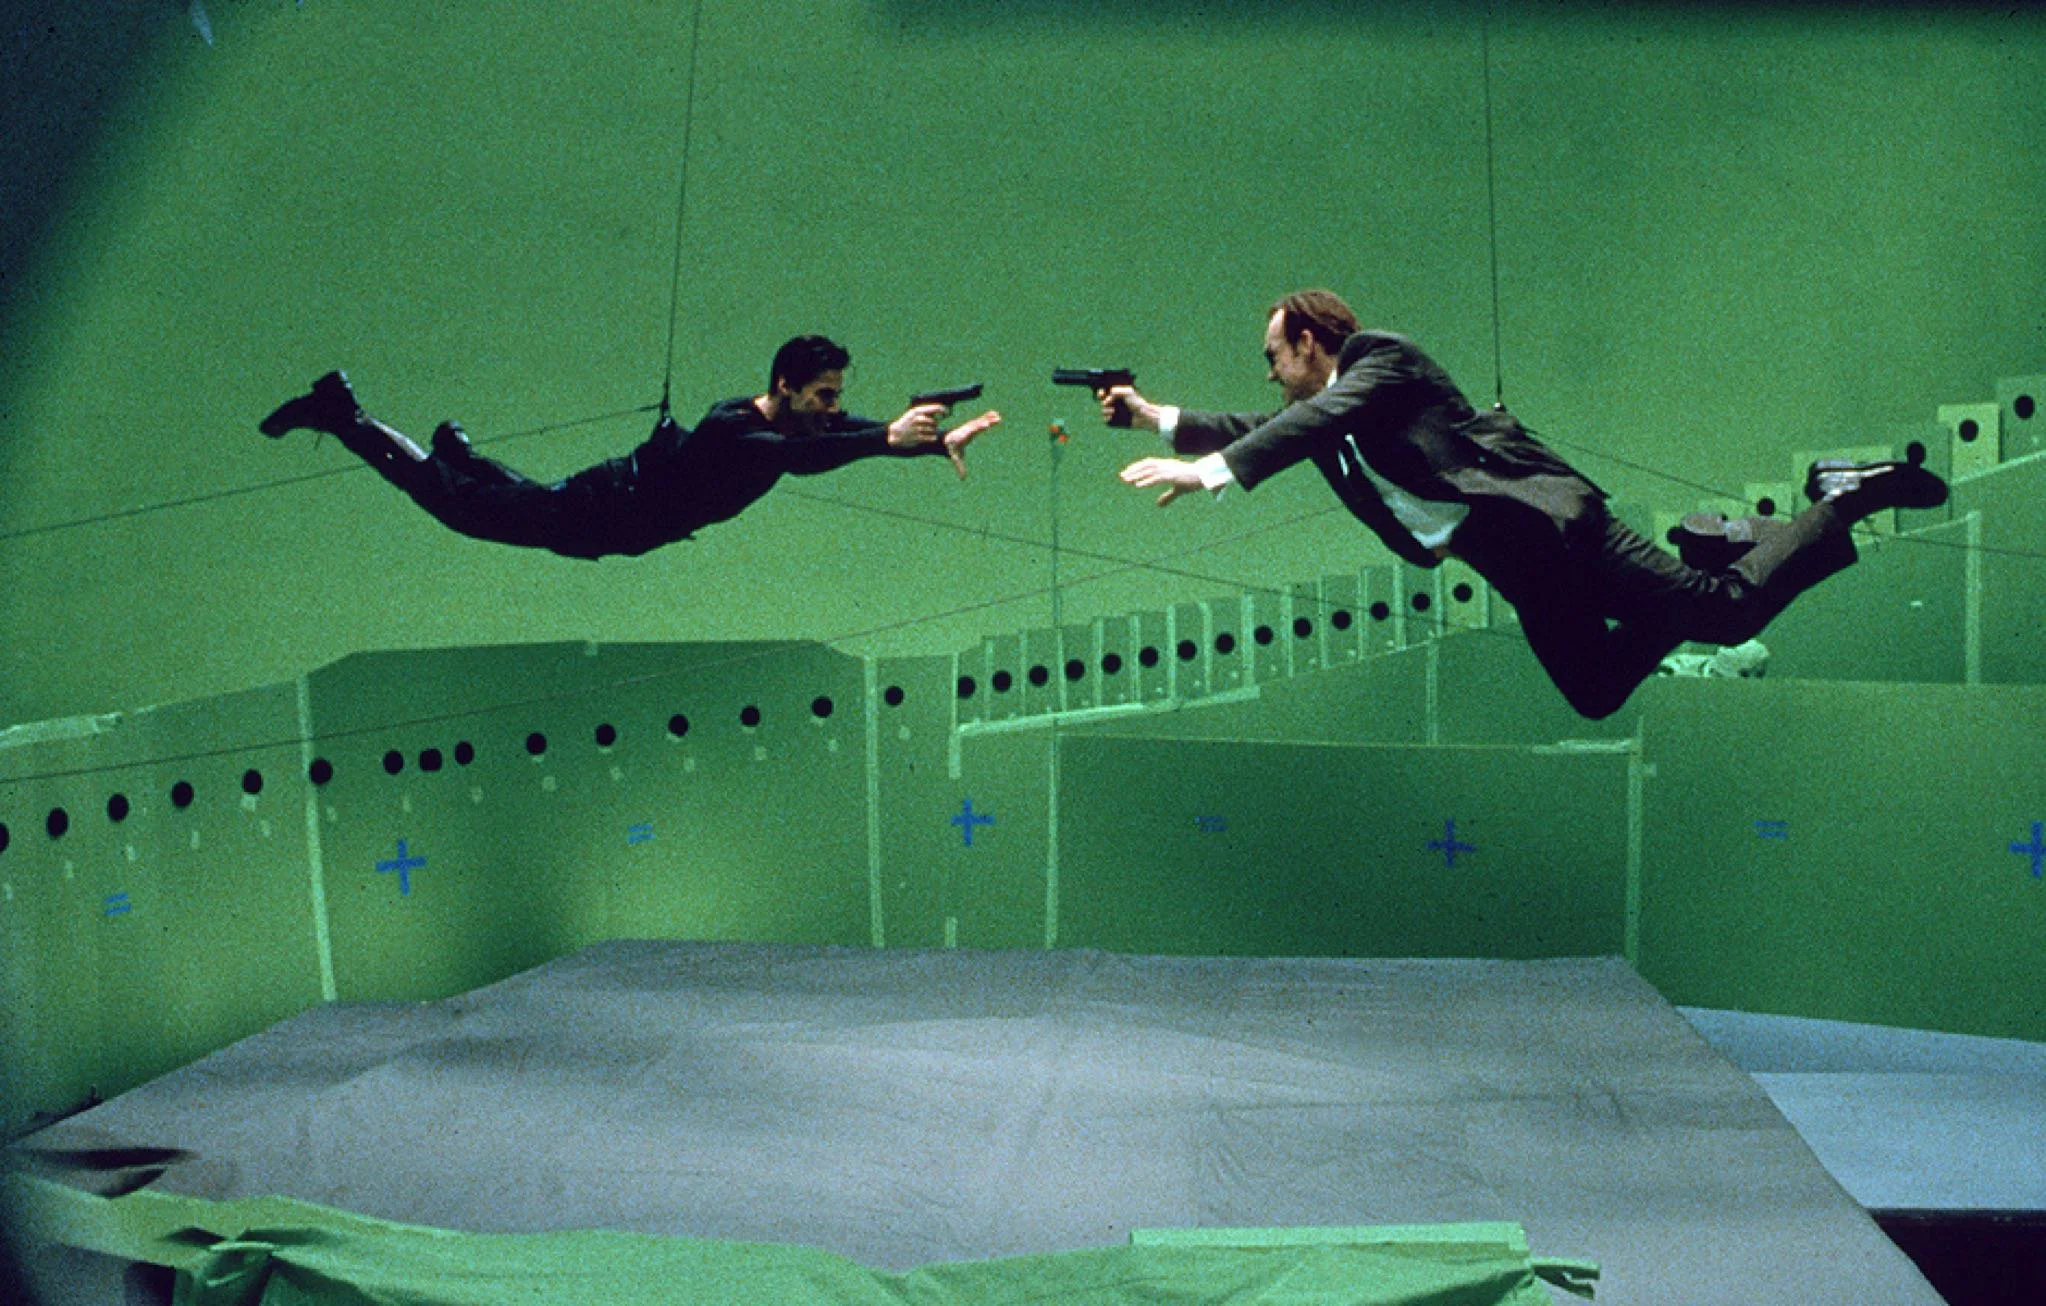
\includegraphics[width=150px]{pictures/green-screen.png}
}

% Document
\begin{document}

\newcommand{\funcname}[1]{%
\texttt{\textcolor{RoyalBlue}{#1}}%
}

\newcommand{\funcarg}[1]{%
\texttt{\textcolor{Periwinkle}{#1}}%
}

\newcommand{\localname}[1]{%
\texttt{\textcolor{Periwinkle}{#1}}%
}

\newcommand{\typename}[1]{%
\texttt{\textcolor{BrickRed}{#1}}%
}

\newcommand{\regname}[1]{%
  \texttt{\textcolor{Periwinkle}{$\langle$#1$\rangle$}}%
}

% Include for tikz diagrams
\newif\ifHexadecimal
\newif\ifShowAddress
\newif\ifNextArrow
\pgfkeys{
/stackDiagram/.is family,
/stackDiagram,
default/.style={wordSize=8,xFactor=3.8,yFactor=1,stackOffset=8,colorOpacity=50,showAddress=false},
wordSize/.estore in=\wordSize,
xFactor/.estore in=\xFactor,
yFactor/.estore in=\yFactor,
stackOffset/.estore in=\stackOffset,
colorOpacity/.estore in=\colorOpacity,
showAddress/.is if=ShowAddress,
%
/stackFrame/.is family,
/stackFrame,
default/.style={color=GreenYellow,opacity=1},
color/.estore in=\sfColor,
opacity/.estore in=\sfOpacity,
%
/frameLocal/.is family,
/frameLocal,
default/.style={hex=false,opacity=1},
hex/.is if=Hexadecimal,
opacity/.estore in=\flOpacity,
%
/funFrame/.is family,
/funFrame,
default/.style={name={},color=GreenYellow,opacity=1,retaddr={}},
name/.estore in=\ffName,
color/.estore in=\ffColor,
opacity/.estore in=\ffOpacity,
retaddr/.estore in=\ffRetAddr,
%
/trapFrame/.is family,
/trapFrame,
default/.style={name={},color=RedOrange,opacity=1,handler={},next=0},
name/.estore in=\tfName,
color/.estore in=\tfColor,
opacity/.estore in=\tfOpacity,
handler/.estore in=\tfHandler,
next/.estore in=\tfNext,
nextarrow/.is if=NextArrow,
%
/showRegister/.is family,
/showRegister,
default/.style={color=Black,opacity=1,offset=0},
color/.estore in=\srColor,
opacity/.estore in=\srOpacity,
offset/.estore in=\srOffset,
}

\newcommand{\hexToDecInto}[2]{%
	\StrGobbleLeft{#2}{2}[\stepA]%
	\StrSubstitute{\stepA}{a}{A}[\stepB]%
	\StrSubstitute{\stepB}{b}{B}[\stepC]%
	\StrSubstitute{\stepC}{c}{C}[\stepD]%
	\StrSubstitute{\stepD}{d}{D}[\stepE]%
	\StrSubstitute{\stepE}{e}{E}[\stepF]%
	\StrSubstitute{\stepF}{f}{F}[\out]%
	\edef#1{\xintHexToDec{\out}}
}

\newcommand{\isBigNumber}[1]{\pdfmatch{^[0-9]+$}{#1}}
\newcommand{\isBigNum}[1]{\ifthenelse{\pdfmatch{^[0-9]+$}{#1} = 1}{red}{blue}}

\tikzset{
addr/.style={right,color=black!50,fill=white,font={\ttfamily\tiny},xshift=1}
}


\newenvironment{stackDiagram}[3][]{%
% #2 -> StackBegin
% #3 -> StackEnd
\pgfkeys{/stackDiagram,default,#1}%
%
\newcommand\stackBegin{\xinteval{#2 + \stackOffset}}
\newcommand\stackEnd{\xinteval{#3 - \stackOffset * 2}}
}%
{}

\newcommand{\debugAxis}{{
\newcommand\x{-1}
\draw [dashed,gray!50] (\x, 0) -- (\x, -10);
\foreach \i in {0, -1, ..., -10} {
	\draw (\x, \i) node [font=\tiny] {$\bullet$};
	\draw (\x, \i) node [left,font=\tiny] {\i};
}
}}


\newcommand{\yOffset}[1]{{
% #1 -> Addr
\xintfloateval{-(((\stackBegin - (#1)) // \wordSize) * \yFactor)}
}}


\newcommand{\debugAddr}[2][blue]{{
% #1 -> FontColor (optional)
% #2 -> Addr

\newcommand\debugAddrX{-1}
\newcommand\debugAddrY{\yOffset{#2}}

\draw (\debugAddrX, \debugAddrY) node [color=#1] {$\bullet$};
}}


\newcommand{\debugCoord}{{
\newcommand\debugCoordX{-1}
\newcommand\debugCoordDiff{\xinteval{\stackBegin - \stackEnd}}

\foreach \i in {0, 8, ..., \debugCoordDiff} {
	\newcommand\debugCoordAddrIt{\xinteval{\stackBegin - \i}}

	\debugAddr{\debugCoordAddrIt}

	\newcommand\debugCoordAddrY{\yOffset{\debugCoordAddrIt}}
	\draw (\debugCoordX, \debugCoordAddrY) node [left,font=\small]{\xintDecToHex{\debugCoordAddrIt} is at \debugCoordAddrY};
}
}}

% TODO optional pgfkey for left/right
\newcommand{\coordAtLeft}[2]{{
% #1 -> Name
% #2 -> Address

\tikzmath{
\y = \yOffset{#2};
\y = \y + 0.5 * \yFactor;
}

\coordinate (#1) at (0, \y);
}}

\newcommand{\coordAtRight}[2]{{
% #1 -> Name
% #2 -> Address

\tikzmath{
\y = \yOffset{#2};
\y = \y + 0.5 * \yFactor;
}

\coordinate (#1) at (\xFactor, \y);
}}

\newcommand{\colorWithOpacity}[1]{%
#1!\colorOpacity%
}

\newcommand\callStack{{
\tikzmath{
\Ax = 0; \Ay = \yOffset{\stackBegin};
\Bx = 1 * \xFactor; \By = \Ay;
\Cx = \Bx; \Cy = \yOffset{\stackEnd};
\Dx = \Ax; \Dy = \Cy;
}

\coordinate (stackTL) at (\Ax, \Ay);
\coordinate (stackTR) at (\Bx, \By);
\coordinate (stackBR) at (\Cx, \Cy);
\coordinate (stackBL) at (\Dx, \Dy);

\draw [dashed] (stackTL)
-- (stackTR) node [addr] {\ifShowAddress 0xFFFFFFFFFFFF \fi}
-- (stackBR) node [addr] {\ifShowAddress 0x0 \fi }
-- (stackBL)
-- cycle;

\ifnum \stackOffset > 0
\tikzmath{
\Ax = 0; \Ay = \yOffset{\stackBegin};
\Bx = 1 * \xFactor; \By = \Ay;
\Cx = \Bx; \Cy = \yOffset{\stackBegin - \stackOffset};
\Dx = \Ax; \Dy = \Cy;
}

\fill [pattern=crosshatch,opacity=0.4] (\Ax, \Ay) -- (\Bx, \By) -- (\Cx, \Cy) -- (\Dx,\Dy) -- cycle;
\fi
}}


\newenvironment{stackFrame}[3][]{
% #2 -> FrameBegin
% #3 -> FrameEnd
\pgfkeys{/stackFrame,default,#1}

\newcommand\sfBegin{#2}
\newcommand\sfEnd{#3}

\tikzmath{
\Ax = 0; \Ay = \yOffset{#2};
\Bx = 1 * \xFactor; \By = \Ay;
\Cx = \Bx; \Cy = \yOffset{#3};
\Dx = \Ax; \Dy = \Cy;
}

\filldraw[fill=\colorWithOpacity{\sfColor},opacity=\sfOpacity,draw=black]
	(\Ax, \Ay)
	-- (\Bx, \By) node [addr] {\ifShowAddress 0x\xintDecToHex{#2} \fi}
	-- (\Cx, \Cy) node [addr] {\ifShowAddress 0x\xintDecToHex{#3} \fi}
	-- (\Dx, \Dy)
	--cycle;

\newcommand\total{\xintiieval{#2 - #3 - 1}}
\foreach \i in {0, 8, ..., \total} {
\ifnum \i>0
	\draw [thin,dashed,gray,opacity=0.5] (0, \yOffset{#2 - \i}) -- (\xFactor, \yOffset{#2 - \i});
\fi
}
}{}


\newcommand\frameName[1]{{
\tikzmath{
\Lx = 1 * \xFactor;
\Lyt= \yOffset{\sfBegin}; \Lyb = \yOffset{\sfEnd};
\Ly = (\Lyt + \Lyb) / 2;
}

% FIXME fill=\colorWithOpacity{\sfColor}
\draw (\Lx, \Ly) node [above,rotate=90,opacity=\sfOpacity,yshift=1] {#1};
}}


\newcommand\frameLocalAt[3][]{{
% #2 -> localAddr
% #3 -> localValue
\pgfkeys{/frameLocal,default,#1}

\tikzmath{
\Ax = \xFactor * 0.5;
\Ay = \yOffset{#2}; \Ay = \Ay + 0.5 * \yFactor;
}

\ifHexadecimal
\draw (\Ax, \Ay) node [opacity=\flOpacity] {0x\xintDecToHex{#3}};
\else
\draw (\Ax, \Ay) node [opacity=\flOpacity] {#3};
\fi
}}


\newcommand\frameLocal[3][]{{
% #2 -> localOffset
% #3 -> localValue
\pgfkeys{/frameLocal,default,#1}

\newcommand\sfLocalAddr{%
\xintfloateval{\sfBegin - ((#2 + 1) * \wordSize)}%
}
\frameLocalAt[#1,opacity=\sfOpacity]{\sfLocalAddr}{#3}
}}


\newcommand\frameReturnAddr[2][]{{
% #2 -> frameReturnAddr
\pgfkeys{/frameLocal,default,#1}

\frameLocal[#1]{0}{#2}
}}


\newcommand{\pointerTo}[2]{{
% #1 -> ptrAddr
% #2 -> ptrValue

\frameLocalAt[hex=true]{#1}{#2}

\tikzmath{
\Ax = 0;
\Ay = \yOffset{#1}; \Ay = \Ay + 0.5 * \yFactor;
\Bx = 0;
\By = \yOffset{#2}; \By = \By + 0.5 * \yFactor;
\Cx = -0.5; \Cy = (\Ay + \By) / 2;
}
 
\draw [darkgray] (0.5, \Ay) -- (\Ax, \Ay);
\draw [darkgray,rounded corners] (\Ax, \Ay) -| (\Cx, \Cy);
\draw [darkgray,->,rounded corners] (\Cx, \Cy) |- (\Bx, \By);
}}


\newenvironment{funFrame}[3][]{
% #2 -> ffBegin
% #3 -> ffEnd
\pgfkeys{/funFrame,default,#1}

\begin{stackFrame}[color=\ffColor,opacity=\ffOpacity]{#2}{#3}
\IfStrEq{\ffName}{}
{}
{\funName{\ffName}}
\IfStrEq{\ffRetAddr}{}
{}
{\funReturnAddr{\ffRetAddr}}
}
{\end{stackFrame}}


\newcommand\funName[1]{{
\frameName{#1}
}}


\newcommand\funReturnAddr[2][]{{
% #2 -> funReturnAddr
\pgfkeys{/frameLocal,default,#1}

\frameReturnAddr[#1]{#2}
}}

\newcommand\showRegister[3][] {
% #2 -> regName
% #3 -> regAddr
\pgfkeys{/showRegister,default,#1}%

\tikzmath{
\Ax = -0.3 + \srOffset;
\Ay = \yOffset{#3}; \Ay = \Ay + 0.5 * \yFactor;
\Bx = 0;
\By = \yOffset{#3}; \By = \By + 0.5 * \yFactor;
}

\draw [->,>=stealth,color=\srColor] (\Ax, \Ay)
	node [draw,fill=white,rounded corners,left] {#2}
	-- (\Bx, \By);
}


\newcommand{\trapFrame}[2][]{{
% #2 -> trapAddr
\pgfkeys{/trapFrame,default,#1}

\begin{stackFrame}[color=\tfColor,opacity=\tfOpacity]{#2}{\xinteval{#2 - 2 * \wordSize}}
\frameName{\tfName}
\frameLocal{0}{\tfHandler}

\ifNextArrow
\pointerTo{\xinteval{#2 - \wordSize}}{\xinteval{\tfNext - \wordSize}}
\else
\IfStrEq{\tfNext}{}
{}

% FIXME pfgkeys should expand hex with commands
{\ifthenelse{\isBigNumber{\tfNext} = 1}
{\frameLocal[hex=true]{1}{\tfNext}}
{\frameLocal[hex=false]{1}{\tfNext}}}
\fi
\end{stackFrame}
}}

\pgfkeys{
/domainState/.is family,
/domainState,
default/.style={pos={(0,-4)},xFactor=3.8,yFactor=0.05},
pos/.estore in=\pos,
xFactor/.estore in=\xFactor,
yFactor/.estore in=\yFactor,
}

\newcommand{\domainStateCommon}[1][]{
\pgfkeys{/domainState,default,#1}%

\tikzset{
header/.style={
anchor=north west,
minimum width={\xFactor * 1cm},
text height={\yFactor * 1cm},
fill=black!10},
fields/.style={
ampersand replacement=\&,
matrix anchor=north,
nodes={anchor=base,align=left,inner xsep=0cm, inner ysep=0.1cm},
text width={((\xFactor * 1cm) / 2)},
text height={\yFactor * 1cm},
inner xsep=0cm,
inner ysep=0cm}
}

\node (header) at \pos [header] {caml\_domain\_state};
}

\newcommand{\domainState}[2][]{{
% #2 -> exn_handler value

\domainStateCommon[#1]{}

\matrix (fields) [fields] at (header.south)
{
\node (exnHandlerLeft) {exn_handler:}; \& \node (exnHandlerRight) {0x\xintDecToHex{#2}}; \\
};

\draw [draw,fill=black,opacity=0.05] (header.north west) rectangle (fields.south east);
}}

\newcommand{\domainStateBacktrace}[4][]{{
% #2 -> exn_handler value
% #3 -> backtrace_buffer
% #4 -> backtrace_pos

\domainStateCommon[#1]{}

\matrix (fields) [fields] at (header.south)
{
\node (exnHandlerLeft) {exn_handler:}; \& \node (exnHandlerRight) {0x\xintDecToHex{#2}}; \\
\node {backtrace\_buffer:}; \& \node {#3}; \\
\node {backtrace\_pos:}; \& \node {#4}; \\
};

\draw [draw,fill=black,opacity=0.05] (header.north west) rectangle (fields.south east);
}}



\newcommand\frameSubsection[2]{
\begin{frame}
\vfill
\centering
\begin{beamercolorbox}[sep=8pt,center,shadow=true,rounded=true]{title}
  \usebeamerfont{title}\insertsectionhead\par%
  \smallskip
  \usebeamerfont{subtitle}\insertsubsectionhead\par%
\end{beamercolorbox}
\ifthenelse{\equal{#1}{}}{}{
  \smallskip
  \begin{figure}
    \includegraphics[width=350px]{#1}
    \ifthenelse{\equal{#2}{}}{}{
      \caption*{#2}
    }
  \end{figure}
}
\vfill
\end{frame}
}

\newcommand\frameSubsectionTakeaway{%
\frameSubsection{pictures/Trinity.png}{}%
}


% Title page frame
\begin{frame}
  \titlepage
\end{frame}

\section*{Introduction}
\begin{frame}{Introduction}{What to expect from this talk?}
  \begin{itemize}
    \item This talk is not about \emph{how} to use exceptions in OCaml; it's assumed you already know how to use them.
    \item It's about understanding \emph{what happens} at the lowest level when an exception is raised and when it's caught.\\
      How are OCaml exceptions \emph{implemented} in native code?
    \item OCaml exceptions are said to be particularly fast; how is it achieved?
    \bigskip
    \item There will hopefully be valuable takeaways, even if you don't care about the implementation details.
  \end{itemize}
\end{frame}


\begin{frame}{Introduction}{Who and why?}
  \begin{itemize}
    \item Fabrice (@fabbing on Github) from the compiler-backend team
    \item Ran into exceptions on two tasks: frame-pointers and the thread sanitizer support\footnotemark[1] in OCaml 5
    \bigskip
    \item I like to understand how things work: hopefully, you too! \begin{tiny}Otherwise, this may be quite boring\dots\end{tiny}
    \item Grasping the implementation will corroborate information from the takeaway slides
    \bigskip
    \item Disclaimer: I'm more confident in my knowledge of the runtime than the compiler
  \end{itemize}
  \footnotetext[1]{\url{https://github.com/OlivierNicole/ocaml-tsan}}
\end{frame}


\begin{frame}{Introduction}{Nitty-gritty details}
  There is good news and bad news about what happens with exceptions\ldots
  \begin{exampleblock}<4->{Good news}
    \setlength{\textwidth}{0.6\textwidth}
    \begin{itemize}
      \item<4-> Most of it is architecture specific: the implementation depends on the target machine
      \item<5-> So there will be a lot of x86-64 assembly code!
    \end{itemize}
  \end{exampleblock}
  \begin{alertblock}<2->{Bad news}
    \begin{itemize}
      \item<2-> Some of it happens at runtime in\dots the runtime.
      \item<3-> The runtime uses C code!
    \end{itemize}
  \end{alertblock}
\end{frame}


% Outline frame
\begin{frame}{Outline}{Fasten your seatbelt and brace for impact!}
  \tableofcontents
\end{frame}


\section{Assembly}
\begin{tikzpicture}[font=\sffamily\tiny]
\input{../src/assembly/gdb.out}

\begin{stackDiagram}[yFactor=0.5,showAddress=true]{\doAsmBegin}{\sayHelloEnd}
\callStack

\ifthenelse{\step=1 \or \step=8}{
\begin{funFrame}[name=do\_asm,color=GreenYellow]{\doAsmBegin}{\doAsmSavedRbp}
}{}
\ifthenelse{\step>1 \and \step<5}{
\begin{funFrame}[name=do\_asm,color=GreenYellow]{\doAsmBegin}{\rspStepA}
}{}
\ifthenelse{\step=5}{
\begin{funFrame}[name=do\_asm,color=GreenYellow]{\doAsmBegin}{\rspStepB}
}{}
\ifthenelse{\step>5 \and \step<8}{
\begin{funFrame}[name=do\_asm,color=GreenYellow]{\doAsmBegin}{\rspStepA}
}{}
\funReturnAddr{\doAsmRetaddr}
\frameLocal{1}{saved RBP}
\ifthenelse{\step>2 \and \step<8}{
\frameLocal{3}{\doAsmLocalTwo}
}{}
\ifthenelse{\step>3 \and \step<8}{
\frameLocal{2}{\doAsmLocalOne}
}{}
\ifthenelse{\step=5}{
\frameLocal{4}{\doAsmLocalThree}
}{}
\end{funFrame}

\ifthenelse{\step=7}{
\begin{funFrame}[name=say\_hello,color=YellowGreen]{\sayHelloBegin}{\sayHelloEnd}
\funReturnAddr{\sayHelloRetaddr}
\frameLocal{1}{saved RBP}
\end{funFrame}
}{}



\ifthenelse{\step=1}{
\showRegister{RSP}{\doAsmSavedRbp}
}{}
\ifthenelse{\step>1 \and \step<5}{
\showRegister[color=Black!25]{RSP}{\doAsmSavedRbp}
\showRegister{RSP}{\rspStepA}
}{}
\ifthenelse{\step=5}{
\showRegister[color=Black!25]{RSP}{\rspStepA}
\showRegister{RSP}{\rspStepB}
}{}
\ifthenelse{\step=6}{
\showRegister[color=Black!25]{RSP}{\rspStepB}
\showRegister{RSP}{\rspStepC}
}{}
\ifthenelse{\step=7}{
\showRegister[color=Black!25]{RSP}{\rspStepC}
\showRegister{RSP}{\sayHelloEnd}
}{}
\ifthenelse{\step=8}{
\showRegister[color=Black!25]{RSP}{\rspStepC}
\showRegister{RSP}{\doAsmSavedRbp}
}{}


\end{stackDiagram}
\end{tikzpicture}


\section{Catching exceptions}
%
% Exceptions are values
%
\subsection{Exceptions are values}
\frameSubsection{pictures/Potentials.png}{- There is no spoon.}

% https://dev.realworldocaml.org/error-handling.html#exceptions
% https://dev.realworldocaml.org/runtime-memory-layout.html
% https://v2.ocaml.org/manual/extensiblevariants.html
\begin{frame}{Exceptions are ordinary values}
\begin{itemize}
\item Exceptions are ordinary values\footnotemark
\item No longer special: an extensible variant type (\text{``}not fully defined in one place\text{''})
\item \mintinline{ocaml}{exception Exc} is equivalent to \mintinline{ocaml}{type exn += Exc of int}
\item Like variants, if the exception has no parameter, memory allocation isn't needed
\item Exceptions with parameter (\mintinline{ocaml}{exception <name> of <type>}) need heap allocation
\end{itemize}
\footnotetext[1]{https://dev.realworldocaml.org/error-handling.html\#exceptions}
\footnotetext[2]{https://v2.ocaml.org/manual/extensiblevariants.html}
\end{frame}


%
% Takeaway #1
%
\subsection*{Takeaway \#1}
\frameSubsectionTakeaway{}
\begin{frame}<1>[label=takeaway]
\frametitle{Takeaway}
\begin{enumerate}
\item<1-> No allocation to create an exception value for exception without parameter
\item<2-> No allocation to install an exception handler
\item<3-> Jumping to the last installed exception handler is done in constant time $O(1)$
\only<3>{
\begin{itemize}
\item No matter how many stack frames between the raising point and the exception handler
\item Unless... see \#4
\end{itemize}
}
\item<4-> Catching an exception is linear complexity $O(n)$ in terms of number of installed exception \emph{handlers}
\only<4>{
\begin{itemize}
\item Algorithm: trap linked-list traversal
\begin{itemize}
\item Discard stack frames up to the last installed handler
\item Execute the handler's pattern matching
\item If no match, re-raise the exception
\end{itemize}
\item Catching an exception early, in terms of traversed handlers, is cheaper
\end{itemize}
}
\item<5-> Compiling with debug information (\mintinline{sh}{-g}) and activating backtrace collection (\mintinline{sh}{OCAMLRUNPARAM=b} or \mintinline{ocaml}{Printexc.record_backtrace b}) causes complexity of jumping to an handler to be $O(n)$ in terms of number of stack frames
\only<5>{
\begin{itemize}
\item Use \funcname{raise\_notrace} to inhibit the backtrace collection
\end{itemize}
\bigskip
\listocaml[firstline=205,lastline=210]{../ocaml/otherlibs/dynlink/dynlink\_compilerlibs/misc.ml}{otherlibs/dynlink/dynlink\_compilerlibs/misc.ml:205}
}
\end{enumerate}
\end{frame}



%
% Exception handlers
%
\subsection{Exception handlers}
\frameSubsection{pictures/Agents.png}{} %{- Deploy the sentinels. Immediately.}

% https://v2.ocaml.org/manual/expr.html#pattern-matching
\begin{frame}[fragile]{Syntax}{BNF\footnotemark}
\begin{grammar}
<expr> ::= <value-path>
  \alt \dots
	\alt `match' <expr> `with' <pattern-matching>
	\alt `try' <expr> `with' <pattern-matching>
  \alt \dots

<pattern-matching> ::= [ `|' ] <pattern> [`when' <expr>] `->' <expr> ( `|' <pattern> [`when' <expr>] `->' <expr> )

<pattern> ::= <value-name>
	\alt \dots
	\alt `exception' <pattern>
	\alt \dots
\end{grammar}
\footnotetext[1]{https://v2.ocaml.org/manual/expr.html\#pattern-matching}
\end{frame}

\begin{frame}{Example of exception handler}{Introduction}
\begin{columns}[c]
\begin{column}{0.6\textwidth}
\begin{itemize}
\item To catch exceptions, an exception handler is needed
\item Let's see the machinery involved in installing (and removing!) one
\end{itemize}
\end{column}
\begin{column}{0.4\textwidth}
\listocaml{../src/trap/trap.ml}{trap/trap.ml}
\end{column}
\end{columns}
\end{frame}

\begin{frame}{Example of exception handler}{Source code}
\begin{columns}[c]
\begin{column}{0.6\textwidth}
\begin{itemize}
\item A custom exception type (\typename{ExnA})
\item \funcname{main} is called by \funcname{camlTrap\_\_entry} with \funcarg{42} as argument
\item \funcname{main} installs an exception handler for \typename{ExnA}
\item \funcname{main} returns its argument incremented by one
\item \funcname{maybe\_raise} raises \typename{ExnA} if the \localname{Should.raise} returns \funcarg{true}
\item Otherwise \funcname{maybe\_raise} returns its argument incremented by one
\end{itemize}
\end{column}
\begin{column}{0.4\textwidth}
\listocaml{../src/trap/trap.ml}{trap/trap.ml}
\end{column}
\end{columns}
\end{frame}

\begin{frame}{Example of exception handler}{CMM, linear and assembly}
\begin{columns}[c]
\begin{column}{0.6\textwidth}
\begin{itemize}
% FIXME Get a better definition
\item CMM is the lowest structured representation of code
\item Linear is below CMM and common to all native codes
\item The assembly emitted from linear is architecture-specific (amd64 target for x86-64 CPU)
\end{itemize}
\end{column}
\begin{column}{0.4\textwidth}
\listocaml[firstline=8,lastline=11]{../src/trap/trap.ml}{trap/trap.ml}
\end{column}
\end{columns}
\end{frame}

\begin{frame}{Example of exception handler}{Exception handler's code}
\begin{columns}[c]
\begin{column}{0.5\textwidth}
\begin{itemize}
\item<1-> In case of exception in the body of the \mintinline{ocaml}{try ... with}, execution flow must be redirected to the handler code (where the pattern matching happens)
\item<1-> To this end, the \mintinline{ocaml}{try ... with} installs a trap on the stack
\begin{itemize}
\item<1-> Installs the trap before executing the body (at the \mintinline{ocaml}{try})
\item<1-> Removes the trap after succesfull execution of the body (at the \mintinline{ocaml}{with})
\end{itemize}
\item<2-> CMM doesn't let us witness those operations
\item<3-> But linear does!
\item<4-> Although we can't see the trap implementation (since it's architecture-specific)
\item<5-> We have to go deeper: let's look at the disassembly of \funcname{main}
\end{itemize}
\smallskip
\listocaml[firstline=8,lastline=11,highlightlines={9-10}]{../src/trap/trap.ml}{trap/trap.ml}
\end{column}
\begin{column}{0.5\textwidth}
\only<1-2>{\listcmm[highlightlines={2-7}]{../src/trap/camlTrap\_\_main\_273.cmm}{main CMM}}%
\only<3>{\listlinear[highlightlines={5-20}]{../src/trap/camlTrap\_\_main\_273.linear}{main linear}}%
\only<4>{\listocaml[firstline=255,lastline=268]{../ocaml/asmcomp/linearize.ml}{asmcomp/linearize.ml:255}}%
\only<5->{\listobjdump[firstline=2,lastline=36]{../src/trap/camlTrap\_\_main\_273.objdump}{main disassembly}}%
\end{column}
\end{columns}
\end{frame}

\begin{frame}{Example of exception handler}{Stack overflow handling}
\begin{columns}[c]
\begin{column}{0.5\textwidth}
\onslide*<1>{
\begin{itemize}
\item Let's ignore the stack overflow handling
\item OCaml stack size is limited (always on a fiber now!)
\item Functions that need stack space must check that creating the stack frame wouldn't cause a stack-overflow
\item If the frame would overflow, the stack (fiber) has to be reallocated
\end{itemize}
\bigskip
\listocaml[firstline=8,lastline=11]{../src/trap/trap.ml}{trap/trap.ml}
}
\onslide*<2>{
\listocaml[firstline=906,lastline=915]{../ocaml/asmcomp/amd64/emit.mlp}{asmcomp/amd64/emit.mlp:906}
\listocaml[firstline=921,lastline=931]{../ocaml/asmcomp/amd64/emit.mlp}{asmcomp/amd64/emit.mlp:921}
}
\end{column}
\begin{column}{0.5\textwidth}
\listobjdump[firstline=2,lastline=36,highlightlines={2-4,33-36}]{../src/trap/camlTrap\_\_main\_273.objdump}{main disassembly}
\end{column}
\end{columns}
\end{frame}


%
% Installing a trap
%
\subsection{Installing a trap}
\frameSubsection{pictures/Mouse.png}{- It's a trap, get out! - Oh, no!}


\begin{frame}{Example of exception handler}{Frame setup}
\begin{columns}
\begin{column}{0.5\textwidth}
\onslide*<1-2>{
\begin{itemize}
\item<1-> \funcname{entry} called \funcname{main} with \mintinline{gas}{call camlTrap__main_273}: the return address into \funcname{entry} is pushed on the stack, and execution jumps to \funcname{main}
\item<2-> Some stack space is reserved for storing \funcname{main}'s argument
\end{itemize}
\bigskip
}%
\onslide*<3>{
\listobjdump[firstline=5,lastline=29,highlightlines={5-6}]{../src/trap/camlTrap\_\_main\_273.objdump}{main disassembly}
\medskip
}%
\listocaml[firstline=8,lastline=11,highlightlines=8]{../src/trap/trap.ml}{trap/trap.ml}
\end{column}
\begin{column}{0.5\textwidth}
\centering
\onslide*<1>{\providecommand\step{1}\begin{tikzpicture}[font=\sffamily\tiny]
\input{../src/trap/gdb.out}

\newcommand\trapEnd{\xinteval{\trapBegin - 2 * \wordSize}}
\newcommand\regRspStepOne{\xinteval{\frameMainBegin - 1 * \wordSize}}
\newcommand\regRspStepTwo{\xinteval{\frameMainBegin - 2 * \wordSize}}
\newcommand\regRspStepThree{\xinteval{\frameMainBegin - 3 * \wordSize}}
\newcommand\regRspStepFour{\xinteval{\frameMainBegin - 4 * \wordSize}}


\begin{stackDiagram}[yFactor=0.4,showAddress=true]{\frameEntryBegin}{\frameMaybeEnd}
\callStack

\begin{funFrame}[name=entry,retaddr=\frameEntryRetaddr,color=GreenYellow]{\frameEntryBegin}{\frameEntryEnd}
\end{funFrame}

\ifthenelse{\step=1}
{\begin{funFrame}[color=YellowGreen]{\frameMainBegin}{\regRspStepOne}}
{\begin{funFrame}[name=main,color=YellowGreen]{\frameMainBegin}{\frameMainEnd}}
\funReturnAddr{\frameMainRetaddr}
\ifthenelse{\step=1}
{}{\frameLocal{1}{\frameMainLocalOne}}
\end{funFrame}


\ifthenelse{\step=3 \or \step=4}
{\frameLocalAt{\regRspStepThree}{\trapHandler}}{}
\ifthenelse{\step=4}
{\frameLocalAt[hex=true]{\regRspStepFour}{\trapNext}}{}
\ifthenelse{\step>4}
{\trapFrame[name=trap,handler=\trapHandler,next=\trapNext,color=WildStrawberry]{\trapBegin}}{}

\ifthenelse{\step=6}{
\begin{funFrame}[name=maybe,color=Green]{\frameMaybeBegin}{\frameMaybeEnd}
\funReturnAddr{\frameMaybeRetaddr}
\frameLocal{1}{\frameMaybeLocalOne}
\end{funFrame}
}{}


\ifthenelse{\step=1}{
\showRegister[color=black!25]{RSP}{\frameMainBegin}
\showRegister{RSP}{\regRspStepOne}
}{}
\ifthenelse{\step=2}{
\showRegister[color=black!25]{RSP}{\regRspStepOne}
\showRegister{RSP}{\regRspStepTwo}
}{}
\ifthenelse{\step=3}{
\showRegister[color=black!25]{RSP}{\regRspStepTwo}
\showRegister{RSP}{\regRspStepThree}
}{}
\ifthenelse{\step>3 \and \step<6}{
\showRegister[color=black!25]{RSP}{\regRspStepThree}
\showRegister{RSP}{\regRspStepFour}
}{}
\ifthenelse{\step=6}{
\showRegister[color=black!25]{RSP}{\regRspStepFour}
\showRegister{RSP}{\frameMaybeEnd}
}{}


\coordinate (bottom) at ($(stackBL) + (0,-0.5)$);

\ifthenelse{\step=4}
{\domainState[pos=(bottom)]{\exnHandlerBeforeTrap}}{}

\ifthenelse{\step>4}{
\domainState[pos=(bottom)]{\exnHandlerAfterTrap}
\coordAtRight{trap}{\exnHandlerAfterTrap}
\draw [->,>=latex] (exnHandlerRight.east) to [out=0,in=0] (trap.east);
}
{}

\end{stackDiagram}
\end{tikzpicture}
}%
\onslide*<2->{\providecommand\step{2}\begin{tikzpicture}[font=\sffamily\tiny]
\input{../src/trap/gdb.out}

\newcommand\trapEnd{\xinteval{\trapBegin - 2 * \wordSize}}
\newcommand\regRspStepOne{\xinteval{\frameMainBegin - 1 * \wordSize}}
\newcommand\regRspStepTwo{\xinteval{\frameMainBegin - 2 * \wordSize}}
\newcommand\regRspStepThree{\xinteval{\frameMainBegin - 3 * \wordSize}}
\newcommand\regRspStepFour{\xinteval{\frameMainBegin - 4 * \wordSize}}


\begin{stackDiagram}[yFactor=0.4,showAddress=true]{\frameEntryBegin}{\frameMaybeEnd}
\callStack

\begin{funFrame}[name=entry,retaddr=\frameEntryRetaddr,color=GreenYellow]{\frameEntryBegin}{\frameEntryEnd}
\end{funFrame}

\ifthenelse{\step=1}
{\begin{funFrame}[color=YellowGreen]{\frameMainBegin}{\regRspStepOne}}
{\begin{funFrame}[name=main,color=YellowGreen]{\frameMainBegin}{\frameMainEnd}}
\funReturnAddr{\frameMainRetaddr}
\ifthenelse{\step=1}
{}{\frameLocal{1}{\frameMainLocalOne}}
\end{funFrame}


\ifthenelse{\step=3 \or \step=4}
{\frameLocalAt{\regRspStepThree}{\trapHandler}}{}
\ifthenelse{\step=4}
{\frameLocalAt[hex=true]{\regRspStepFour}{\trapNext}}{}
\ifthenelse{\step>4}
{\trapFrame[name=trap,handler=\trapHandler,next=\trapNext,color=WildStrawberry]{\trapBegin}}{}

\ifthenelse{\step=6}{
\begin{funFrame}[name=maybe,color=Green]{\frameMaybeBegin}{\frameMaybeEnd}
\funReturnAddr{\frameMaybeRetaddr}
\frameLocal{1}{\frameMaybeLocalOne}
\end{funFrame}
}{}


\ifthenelse{\step=1}{
\showRegister[color=black!25]{RSP}{\frameMainBegin}
\showRegister{RSP}{\regRspStepOne}
}{}
\ifthenelse{\step=2}{
\showRegister[color=black!25]{RSP}{\regRspStepOne}
\showRegister{RSP}{\regRspStepTwo}
}{}
\ifthenelse{\step=3}{
\showRegister[color=black!25]{RSP}{\regRspStepTwo}
\showRegister{RSP}{\regRspStepThree}
}{}
\ifthenelse{\step>3 \and \step<6}{
\showRegister[color=black!25]{RSP}{\regRspStepThree}
\showRegister{RSP}{\regRspStepFour}
}{}
\ifthenelse{\step=6}{
\showRegister[color=black!25]{RSP}{\regRspStepFour}
\showRegister{RSP}{\frameMaybeEnd}
}{}


\coordinate (bottom) at ($(stackBL) + (0,-0.5)$);

\ifthenelse{\step=4}
{\domainState[pos=(bottom)]{\exnHandlerBeforeTrap}}{}

\ifthenelse{\step>4}{
\domainState[pos=(bottom)]{\exnHandlerAfterTrap}
\coordAtRight{trap}{\exnHandlerAfterTrap}
\draw [->,>=latex] (exnHandlerRight.east) to [out=0,in=0] (trap.east);
}
{}

\end{stackDiagram}
\end{tikzpicture}
}%
\end{column}
\end{columns}
\end{frame}

\begin{frame}{Example of exception handler}{Entering the try...with}
\begin{columns}
\begin{column}{0.5\textwidth}
\begin{itemize}
\item Now reaching the expression protected by the exception handler
\begin{itemize}
\item Before executing the call to \funcname{maybe\_raise}, the \mintinline{ocaml}{try ... with} install a trap on the stack: \funcname{push trap}
\item If \funcname{maybe\_raise} completes without error, the trap is removed: \funcname{pop trap}
\end{itemize}
\end{itemize}
\bigskip
\listocaml[firstline=8,lastline=11,highlightlines=9]{../src/trap/trap.ml}{trap/trap.ml}
\end{column}
\begin{column}{0.5\textwidth}
\only<1>{\listcmm[highlightlines=2]{../src/trap/camlTrap\_\_main\_273.cmm}{main CMM}}%
\only<2>{\listlinear[highlightlines=5]{../src/trap/camlTrap\_\_main\_273.linear}{main linear}}%
\only<3>{\listocaml[firstline=837,lastline=850]{../ocaml/asmcomp/amd64/emit.mlp}{asmcomp/amd64/emit.mlp:837}}%
\end{column}
\end{columns}
\end{frame}

\begin{frame}{Constructing the trap}{Handler's address}
\begin{columns}
\begin{column}{0.5\textwidth}
\onslide*<1-2>{
\begin{itemize}
\item<1-> The trap is a two-words object constructed on the stack right after the \funcname{main} frame
\item<1-> It redirects the execution flow to the handler in case of an exception
\item<2-> The address of the handler's code is pushed onto the stack
\item<2-> The handler (pattern matching) code is part of the \funcname{main} function code
\end{itemize}
}
\onslide*<3>{\listocaml[firstline=837,lastline=850,highlightlines={838-846}]{../ocaml/asmcomp/amd64/emit.mlp}{asmcomp/amd64/emit.mlp:837}}
\onslide*<4>{\mintobjdump[firstline=5,lastline=29,highlightlines={7-8,16-27}]{../src/trap/camlTrap\_\_main\_273.objdump}}
\medskip
\listocaml[firstline=8,lastline=11,highlightlines=9]{../src/trap/trap.ml}{trap/trap.ml}
\end{column}
\begin{column}{0.5\textwidth}
\centering
\providecommand\step{3}\begin{tikzpicture}[font=\sffamily\tiny]
\input{../src/trap/gdb.out}

\newcommand\trapEnd{\xinteval{\trapBegin - 2 * \wordSize}}
\newcommand\regRspStepOne{\xinteval{\frameMainBegin - 1 * \wordSize}}
\newcommand\regRspStepTwo{\xinteval{\frameMainBegin - 2 * \wordSize}}
\newcommand\regRspStepThree{\xinteval{\frameMainBegin - 3 * \wordSize}}
\newcommand\regRspStepFour{\xinteval{\frameMainBegin - 4 * \wordSize}}


\begin{stackDiagram}[yFactor=0.4,showAddress=true]{\frameEntryBegin}{\frameMaybeEnd}
\callStack

\begin{funFrame}[name=entry,retaddr=\frameEntryRetaddr,color=GreenYellow]{\frameEntryBegin}{\frameEntryEnd}
\end{funFrame}

\ifthenelse{\step=1}
{\begin{funFrame}[color=YellowGreen]{\frameMainBegin}{\regRspStepOne}}
{\begin{funFrame}[name=main,color=YellowGreen]{\frameMainBegin}{\frameMainEnd}}
\funReturnAddr{\frameMainRetaddr}
\ifthenelse{\step=1}
{}{\frameLocal{1}{\frameMainLocalOne}}
\end{funFrame}


\ifthenelse{\step=3 \or \step=4}
{\frameLocalAt{\regRspStepThree}{\trapHandler}}{}
\ifthenelse{\step=4}
{\frameLocalAt[hex=true]{\regRspStepFour}{\trapNext}}{}
\ifthenelse{\step>4}
{\trapFrame[name=trap,handler=\trapHandler,next=\trapNext,color=WildStrawberry]{\trapBegin}}{}

\ifthenelse{\step=6}{
\begin{funFrame}[name=maybe,color=Green]{\frameMaybeBegin}{\frameMaybeEnd}
\funReturnAddr{\frameMaybeRetaddr}
\frameLocal{1}{\frameMaybeLocalOne}
\end{funFrame}
}{}


\ifthenelse{\step=1}{
\showRegister[color=black!25]{RSP}{\frameMainBegin}
\showRegister{RSP}{\regRspStepOne}
}{}
\ifthenelse{\step=2}{
\showRegister[color=black!25]{RSP}{\regRspStepOne}
\showRegister{RSP}{\regRspStepTwo}
}{}
\ifthenelse{\step=3}{
\showRegister[color=black!25]{RSP}{\regRspStepTwo}
\showRegister{RSP}{\regRspStepThree}
}{}
\ifthenelse{\step>3 \and \step<6}{
\showRegister[color=black!25]{RSP}{\regRspStepThree}
\showRegister{RSP}{\regRspStepFour}
}{}
\ifthenelse{\step=6}{
\showRegister[color=black!25]{RSP}{\regRspStepFour}
\showRegister{RSP}{\frameMaybeEnd}
}{}


\coordinate (bottom) at ($(stackBL) + (0,-0.5)$);

\ifthenelse{\step=4}
{\domainState[pos=(bottom)]{\exnHandlerBeforeTrap}}{}

\ifthenelse{\step>4}{
\domainState[pos=(bottom)]{\exnHandlerAfterTrap}
\coordAtRight{trap}{\exnHandlerAfterTrap}
\draw [->,>=latex] (exnHandlerRight.east) to [out=0,in=0] (trap.east);
}
{}

\end{stackDiagram}
\end{tikzpicture}

\end{column}
\end{columns}
\end{frame}

% TODO notes:
% - trap_{sp_off,barrier_off,barrier_block} -> bytecode
% - backtrace_{pos,active,buffer} -> part II
\begin{frame}{Introducing caml\_domain\_state}{First mention of the runtime!}
\begin{columns}
\begin{column}{0.5\textwidth}
\begin{listing}
\onslide*<1,3>{
\begin{itemize}
\item<1-> \typename{caml\_domain\_state} is a C structure part of the runtime
\item<1-> It holds information useful to the runtime to manage a domain (each domain has its \typename{caml\_domain\_state})
\item<3-> \localname{exn\_hanlder} is a pointer to the \emph{last} installed \typename{trap}
\end{itemize}
}
\onslide*<2>{\mintc[lastline=32]{src/ocaml/domain\_state.h}}
\end{listing}
\end{column}
\begin{column}{0.5\textwidth}
\begin{listing}
\onslide*<2>{\mintc[firstline=32]{src/ocaml/domain\_state.h}}
\onslide*<3->{\listc[highlightlines={7}]{src/ocaml/domain\_state\_abbr.h}{runtime/caml/domain\_state.h}}
\end{listing}
\end{column}
\end{columns}
\end{frame}

\begin{frame}{Constructing the trap}{Saving previous trap address}
\begin{columns}
\begin{column}{0.5\textwidth}
\onslide*<1>{
\begin{itemize}
% TODO grey color
\item The address of the handler's code is pushed onto the stack
% TODO /grey color
\item The value of \localname{exn\_handler} from \typename{caml\_domain\_state} is pushed onto the stack
\item \localname{r14} register points to the current domain's \typename{caml\_domain\_state}
\end{itemize}
}
\onslide*<2>{\listocaml[firstline=837,lastline=850,highlightlines={847-848}]{../ocaml/asmcomp/amd64/emit.mlp}{asmcomp/amd64/emit.mlp:838}}
\onslide*<3>{\mintobjdump[firstline=5,lastline=29,highlightlines=9]{../src/trap/camlTrap\_\_main\_273.objdump}}
\medskip
\listocaml[firstline=8,lastline=11,highlightlines=9]{../src/trap/trap.ml}{trap/trap.ml}
\end{column}
\begin{column}{0.5\textwidth}
\centering
\providecommand\step{4}\begin{tikzpicture}[font=\sffamily\tiny]
\input{../src/trap/gdb.out}

\newcommand\trapEnd{\xinteval{\trapBegin - 2 * \wordSize}}
\newcommand\regRspStepOne{\xinteval{\frameMainBegin - 1 * \wordSize}}
\newcommand\regRspStepTwo{\xinteval{\frameMainBegin - 2 * \wordSize}}
\newcommand\regRspStepThree{\xinteval{\frameMainBegin - 3 * \wordSize}}
\newcommand\regRspStepFour{\xinteval{\frameMainBegin - 4 * \wordSize}}


\begin{stackDiagram}[yFactor=0.4,showAddress=true]{\frameEntryBegin}{\frameMaybeEnd}
\callStack

\begin{funFrame}[name=entry,retaddr=\frameEntryRetaddr,color=GreenYellow]{\frameEntryBegin}{\frameEntryEnd}
\end{funFrame}

\ifthenelse{\step=1}
{\begin{funFrame}[color=YellowGreen]{\frameMainBegin}{\regRspStepOne}}
{\begin{funFrame}[name=main,color=YellowGreen]{\frameMainBegin}{\frameMainEnd}}
\funReturnAddr{\frameMainRetaddr}
\ifthenelse{\step=1}
{}{\frameLocal{1}{\frameMainLocalOne}}
\end{funFrame}


\ifthenelse{\step=3 \or \step=4}
{\frameLocalAt{\regRspStepThree}{\trapHandler}}{}
\ifthenelse{\step=4}
{\frameLocalAt[hex=true]{\regRspStepFour}{\trapNext}}{}
\ifthenelse{\step>4}
{\trapFrame[name=trap,handler=\trapHandler,next=\trapNext,color=WildStrawberry]{\trapBegin}}{}

\ifthenelse{\step=6}{
\begin{funFrame}[name=maybe,color=Green]{\frameMaybeBegin}{\frameMaybeEnd}
\funReturnAddr{\frameMaybeRetaddr}
\frameLocal{1}{\frameMaybeLocalOne}
\end{funFrame}
}{}


\ifthenelse{\step=1}{
\showRegister[color=black!25]{RSP}{\frameMainBegin}
\showRegister{RSP}{\regRspStepOne}
}{}
\ifthenelse{\step=2}{
\showRegister[color=black!25]{RSP}{\regRspStepOne}
\showRegister{RSP}{\regRspStepTwo}
}{}
\ifthenelse{\step=3}{
\showRegister[color=black!25]{RSP}{\regRspStepTwo}
\showRegister{RSP}{\regRspStepThree}
}{}
\ifthenelse{\step>3 \and \step<6}{
\showRegister[color=black!25]{RSP}{\regRspStepThree}
\showRegister{RSP}{\regRspStepFour}
}{}
\ifthenelse{\step=6}{
\showRegister[color=black!25]{RSP}{\regRspStepFour}
\showRegister{RSP}{\frameMaybeEnd}
}{}


\coordinate (bottom) at ($(stackBL) + (0,-0.5)$);

\ifthenelse{\step=4}
{\domainState[pos=(bottom)]{\exnHandlerBeforeTrap}}{}

\ifthenelse{\step>4}{
\domainState[pos=(bottom)]{\exnHandlerAfterTrap}
\coordAtRight{trap}{\exnHandlerAfterTrap}
\draw [->,>=latex] (exnHandlerRight.east) to [out=0,in=0] (trap.east);
}
{}

\end{stackDiagram}
\end{tikzpicture}

\end{column}
\end{columns}
\end{frame}

\begin{frame}{Constructing the trap}{Updating exn\_handler}
\begin{columns}
\begin{column}{0.5\textwidth}
\onslide*<1>{
\begin{itemize}
% TODO grey color
\item The address of the handler's code is pushed onto the stack
\item The value of \localname{exn\_handler} from \typename{caml\_domain\_state} is pushed onto the stack
% TODO /grey color
\item \localname{domain\_state->exn\_hanlder} has to point to the last installed trap
\item Its value is updated to the just-constructed trap's address
\end{itemize}
}
\onslide*<2>{\listocaml[firstline=837,lastline=850,highlightlines=849]{../ocaml/asmcomp/amd64/emit.mlp}{asmcomp/amd64/emit.mlp:849}}
\onslide*<3>{\mintobjdump[firstline=5,lastline=29,highlightlines=10]{../src/trap/camlTrap\_\_main\_273.objdump}}
\medskip
\listocaml[firstline=8,lastline=11,highlightlines=10]{../src/trap/trap.ml}{trap/trap.ml}
\end{column}
\begin{column}{0.5\textwidth}
\centering
\providecommand\step{5}\begin{tikzpicture}[font=\sffamily\tiny]
\input{../src/trap/gdb.out}

\newcommand\trapEnd{\xinteval{\trapBegin - 2 * \wordSize}}
\newcommand\regRspStepOne{\xinteval{\frameMainBegin - 1 * \wordSize}}
\newcommand\regRspStepTwo{\xinteval{\frameMainBegin - 2 * \wordSize}}
\newcommand\regRspStepThree{\xinteval{\frameMainBegin - 3 * \wordSize}}
\newcommand\regRspStepFour{\xinteval{\frameMainBegin - 4 * \wordSize}}


\begin{stackDiagram}[yFactor=0.4,showAddress=true]{\frameEntryBegin}{\frameMaybeEnd}
\callStack

\begin{funFrame}[name=entry,retaddr=\frameEntryRetaddr,color=GreenYellow]{\frameEntryBegin}{\frameEntryEnd}
\end{funFrame}

\ifthenelse{\step=1}
{\begin{funFrame}[color=YellowGreen]{\frameMainBegin}{\regRspStepOne}}
{\begin{funFrame}[name=main,color=YellowGreen]{\frameMainBegin}{\frameMainEnd}}
\funReturnAddr{\frameMainRetaddr}
\ifthenelse{\step=1}
{}{\frameLocal{1}{\frameMainLocalOne}}
\end{funFrame}


\ifthenelse{\step=3 \or \step=4}
{\frameLocalAt{\regRspStepThree}{\trapHandler}}{}
\ifthenelse{\step=4}
{\frameLocalAt[hex=true]{\regRspStepFour}{\trapNext}}{}
\ifthenelse{\step>4}
{\trapFrame[name=trap,handler=\trapHandler,next=\trapNext,color=WildStrawberry]{\trapBegin}}{}

\ifthenelse{\step=6}{
\begin{funFrame}[name=maybe,color=Green]{\frameMaybeBegin}{\frameMaybeEnd}
\funReturnAddr{\frameMaybeRetaddr}
\frameLocal{1}{\frameMaybeLocalOne}
\end{funFrame}
}{}


\ifthenelse{\step=1}{
\showRegister[color=black!25]{RSP}{\frameMainBegin}
\showRegister{RSP}{\regRspStepOne}
}{}
\ifthenelse{\step=2}{
\showRegister[color=black!25]{RSP}{\regRspStepOne}
\showRegister{RSP}{\regRspStepTwo}
}{}
\ifthenelse{\step=3}{
\showRegister[color=black!25]{RSP}{\regRspStepTwo}
\showRegister{RSP}{\regRspStepThree}
}{}
\ifthenelse{\step>3 \and \step<6}{
\showRegister[color=black!25]{RSP}{\regRspStepThree}
\showRegister{RSP}{\regRspStepFour}
}{}
\ifthenelse{\step=6}{
\showRegister[color=black!25]{RSP}{\regRspStepFour}
\showRegister{RSP}{\frameMaybeEnd}
}{}


\coordinate (bottom) at ($(stackBL) + (0,-0.5)$);

\ifthenelse{\step=4}
{\domainState[pos=(bottom)]{\exnHandlerBeforeTrap}}{}

\ifthenelse{\step>4}{
\domainState[pos=(bottom)]{\exnHandlerAfterTrap}
\coordAtRight{trap}{\exnHandlerAfterTrap}
\draw [->,>=latex] (exnHandlerRight.east) to [out=0,in=0] (trap.east);
}
{}

\end{stackDiagram}
\end{tikzpicture}

\end{column}
\end{columns}
\end{frame}


\begin{frame}{OCaml exception trap}{More details to come later!}
\begin{itemize}
\item On amd64, an exception trap could be represented with this C structure
\end{itemize}
\bigskip
\centering{\mintc[firstline=1,lastline=6]{src/ocaml/trap\_partial.c}} % FIXME center
\end{frame}


%
% Takeaway #2
%
\subsection*{Takeaway \#2}
\frameSubsectionTakeaway{}
\againframe<2>{takeaway}


\begin{frame}{Executing the body}{Protected by the try...with}
\begin{columns}
\begin{column}{0.5\textwidth}
\onslide*<1>{
\begin{itemize}
\item Now executing the expression protected by the \mintinline{ocaml}{try ... with}: a call to \funcname{maybe\_raise}
\begin{itemize}
\item Which may complete without exception: the trap has to be removed, and the handler code is not executed
\item Which may raise \typename{ExnA}: execution flow is redirected to the handler code thanks to the trap
\end{itemize}
\end{itemize}
}
\only<2>{\mintcmm[highlightlines=2]{../src/trap/camlTrap\_\_main\_273.cmm}}%
\only<3>{\mintlinear[firstline=2,highlightlines=7]{../src/trap/camlTrap\_\_main\_273.linear}}%
\only<4>{\mintobjdump[firstline=5,lastline=29,highlightlines=11]{../src/trap/camlTrap\_\_main\_273.objdump}}%
\listocaml[firstline=3,lastline=11,highlightlines={3-6,9}]{../src/trap/trap.ml}{trap/trap.ml}
\end{column}
\begin{column}{0.5\textwidth}
\centering
\providecommand\step{6}\begin{tikzpicture}[font=\sffamily\tiny]
\input{../src/trap/gdb.out}

\newcommand\trapEnd{\xinteval{\trapBegin - 2 * \wordSize}}
\newcommand\regRspStepOne{\xinteval{\frameMainBegin - 1 * \wordSize}}
\newcommand\regRspStepTwo{\xinteval{\frameMainBegin - 2 * \wordSize}}
\newcommand\regRspStepThree{\xinteval{\frameMainBegin - 3 * \wordSize}}
\newcommand\regRspStepFour{\xinteval{\frameMainBegin - 4 * \wordSize}}


\begin{stackDiagram}[yFactor=0.4,showAddress=true]{\frameEntryBegin}{\frameMaybeEnd}
\callStack

\begin{funFrame}[name=entry,retaddr=\frameEntryRetaddr,color=GreenYellow]{\frameEntryBegin}{\frameEntryEnd}
\end{funFrame}

\ifthenelse{\step=1}
{\begin{funFrame}[color=YellowGreen]{\frameMainBegin}{\regRspStepOne}}
{\begin{funFrame}[name=main,color=YellowGreen]{\frameMainBegin}{\frameMainEnd}}
\funReturnAddr{\frameMainRetaddr}
\ifthenelse{\step=1}
{}{\frameLocal{1}{\frameMainLocalOne}}
\end{funFrame}


\ifthenelse{\step=3 \or \step=4}
{\frameLocalAt{\regRspStepThree}{\trapHandler}}{}
\ifthenelse{\step=4}
{\frameLocalAt[hex=true]{\regRspStepFour}{\trapNext}}{}
\ifthenelse{\step>4}
{\trapFrame[name=trap,handler=\trapHandler,next=\trapNext,color=WildStrawberry]{\trapBegin}}{}

\ifthenelse{\step=6}{
\begin{funFrame}[name=maybe,color=Green]{\frameMaybeBegin}{\frameMaybeEnd}
\funReturnAddr{\frameMaybeRetaddr}
\frameLocal{1}{\frameMaybeLocalOne}
\end{funFrame}
}{}


\ifthenelse{\step=1}{
\showRegister[color=black!25]{RSP}{\frameMainBegin}
\showRegister{RSP}{\regRspStepOne}
}{}
\ifthenelse{\step=2}{
\showRegister[color=black!25]{RSP}{\regRspStepOne}
\showRegister{RSP}{\regRspStepTwo}
}{}
\ifthenelse{\step=3}{
\showRegister[color=black!25]{RSP}{\regRspStepTwo}
\showRegister{RSP}{\regRspStepThree}
}{}
\ifthenelse{\step>3 \and \step<6}{
\showRegister[color=black!25]{RSP}{\regRspStepThree}
\showRegister{RSP}{\regRspStepFour}
}{}
\ifthenelse{\step=6}{
\showRegister[color=black!25]{RSP}{\regRspStepFour}
\showRegister{RSP}{\frameMaybeEnd}
}{}


\coordinate (bottom) at ($(stackBL) + (0,-0.5)$);

\ifthenelse{\step=4}
{\domainState[pos=(bottom)]{\exnHandlerBeforeTrap}}{}

\ifthenelse{\step>4}{
\domainState[pos=(bottom)]{\exnHandlerAfterTrap}
\coordAtRight{trap}{\exnHandlerAfterTrap}
\draw [->,>=latex] (exnHandlerRight.east) to [out=0,in=0] (trap.east);
}
{}

\end{stackDiagram}
\end{tikzpicture}

\end{column}
\end{columns}
\end{frame}


%
% Removing a trap
%
\subsection{Removing a trap}
\frameSubsection{pictures/bugged.png}{- I think you're bugged.}


\begin{frame}{maybe\_raise terminates normally}{}
\begin{columns}
\begin{column}{0.5\textwidth}
\onslide*<1,3>{
\begin{itemize}
\item<1-> \funcname{maybe\_raise} terminates without exception
\item<1-> Computes its return value and sets it into \regname{RAX}
\item<3-> Increments \regname{RSP} to remove its own stack frame
\end{itemize}
}
\onslide*<2>{
\mintobjdump[firstline=5,lastline=24,highlightlines={21-22}]{../src/noraise/camlNoraise\_\_maybe\_raise\_269.objdump}
}
\onslide*<4>{
\mintobjdump[firstline=5,lastline=24,highlightlines={23-24}]{../src/noraise/camlNoraise\_\_maybe\_raise\_269.objdump}
}
\medskip
\only<1>{\listocaml[firstline=3,lastline=11,highlightlines={6,9}]{../src/noraise/noraise.ml}{noraise/noraise.ml}}%
\onslide*<2->{\listocaml[firstline=3,lastline=6,highlightlines=6]{../src/noraise/noraise.ml}{noraise/noraise.ml}}%
\end{column}
\begin{column}{0.5\textwidth}
\centering
\onslide*<1-2>{\providecommand\step{1}\begin{tikzpicture}[font=\sffamily\tiny]
\input{../src/noraise/gdb.out}

\newcommand\trapEnd{\xinteval{\trapBegin - 2 * \wordSize}}
\newcommand\trapHandlerAddr{\xinteval{\trapBegin - 1 * \wordSize}}


\begin{stackDiagram}[yFactor=0.4,showAddress=true]{\frameEntryBegin}{\frameMaybeEnd}
\callStack

\begin{funFrame}[name=entry,retaddr=\frameEntryRetaddr,color=GreenYellow]{\frameEntryBegin}{\frameEntryEnd}
\end{funFrame}

\begin{funFrame}[name=main,color=YellowGreen]{\frameMainBegin}{\frameMainEnd}
\funReturnAddr{\frameMainRetaddr}
\frameLocal{1}{\frameMainLocalOne}
\end{funFrame}


\ifthenelse{\step=4}{
\trapFrame[name=trap,handler=\trapHandler,next=\trapNext,color=WildStrawberry,opacity=0.25]{\trapBegin}
}{
\trapFrame[name=trap,handler=\trapHandler,next=\trapNext,color=WildStrawberry]{\trapBegin}
}


\ifthenelse{\step=1}
{\begin{funFrame}[name=maybe,color=Green]{\frameMaybeBegin}{\frameMaybeEnd}}
{\begin{funFrame}[name=maybe,color=Green,opacity=0.25]{\frameMaybeBegin}{\frameMaybeEnd}}
\funReturnAddr{\frameMaybeRetaddr}
\frameLocal{1}{\frameMaybeLocalOne}
\end{funFrame}


\ifthenelse{\step=1}{
\showRegister{RSP}{\frameMaybeEnd}
}{}
\ifthenelse{\step=2}{
\showRegister{RSP}{\trapEnd}
\showRegister[color=black!25]{RSP}{\frameMaybeEnd}
}{}
\ifthenelse{\step=3}{
\showRegister{RSP}{\trapHandlerAddr}
\showRegister[color=black!25]{RSP}{\trapEnd}
}{}
\ifthenelse{\step=4}{
\showRegister{RSP}{\frameMainEnd}
\showRegister[color=black!25]{RSP}{\trapHandlerAddr}
}{}


\coordinate (bottom) at ($(stackBL) + (0,-0.5)$);

\ifthenelse{\step<3}{
\domainState[pos=(bottom)]{\exnHandlerAfterTrap}
\coordAtRight{trap}{\exnHandlerAfterTrap}
\draw [->,>=latex] (exnHandlerRight.east) to [out=0,in=0] (trap.east);
}{
\domainState[pos=(bottom)]{\exnHandlerBeforeTrap}
}

\end{stackDiagram}
\end{tikzpicture}
}
\onslide*<3->{\providecommand\step{2}\begin{tikzpicture}[font=\sffamily\tiny]
\input{../src/noraise/gdb.out}

\newcommand\trapEnd{\xinteval{\trapBegin - 2 * \wordSize}}
\newcommand\trapHandlerAddr{\xinteval{\trapBegin - 1 * \wordSize}}


\begin{stackDiagram}[yFactor=0.4,showAddress=true]{\frameEntryBegin}{\frameMaybeEnd}
\callStack

\begin{funFrame}[name=entry,retaddr=\frameEntryRetaddr,color=GreenYellow]{\frameEntryBegin}{\frameEntryEnd}
\end{funFrame}

\begin{funFrame}[name=main,color=YellowGreen]{\frameMainBegin}{\frameMainEnd}
\funReturnAddr{\frameMainRetaddr}
\frameLocal{1}{\frameMainLocalOne}
\end{funFrame}


\ifthenelse{\step=4}{
\trapFrame[name=trap,handler=\trapHandler,next=\trapNext,color=WildStrawberry,opacity=0.25]{\trapBegin}
}{
\trapFrame[name=trap,handler=\trapHandler,next=\trapNext,color=WildStrawberry]{\trapBegin}
}


\ifthenelse{\step=1}
{\begin{funFrame}[name=maybe,color=Green]{\frameMaybeBegin}{\frameMaybeEnd}}
{\begin{funFrame}[name=maybe,color=Green,opacity=0.25]{\frameMaybeBegin}{\frameMaybeEnd}}
\funReturnAddr{\frameMaybeRetaddr}
\frameLocal{1}{\frameMaybeLocalOne}
\end{funFrame}


\ifthenelse{\step=1}{
\showRegister{RSP}{\frameMaybeEnd}
}{}
\ifthenelse{\step=2}{
\showRegister{RSP}{\trapEnd}
\showRegister[color=black!25]{RSP}{\frameMaybeEnd}
}{}
\ifthenelse{\step=3}{
\showRegister{RSP}{\trapHandlerAddr}
\showRegister[color=black!25]{RSP}{\trapEnd}
}{}
\ifthenelse{\step=4}{
\showRegister{RSP}{\frameMainEnd}
\showRegister[color=black!25]{RSP}{\trapHandlerAddr}
}{}


\coordinate (bottom) at ($(stackBL) + (0,-0.5)$);

\ifthenelse{\step<3}{
\domainState[pos=(bottom)]{\exnHandlerAfterTrap}
\coordAtRight{trap}{\exnHandlerAfterTrap}
\draw [->,>=latex] (exnHandlerRight.east) to [out=0,in=0] (trap.east);
}{
\domainState[pos=(bottom)]{\exnHandlerBeforeTrap}
}

\end{stackDiagram}
\end{tikzpicture}
}
\end{column}
\end{columns}
\end{frame}

\begin{frame}{main removes the lingering trap}{Restoring domain\_state->exn\_handler}
\begin{columns}
\begin{column}{0.5\textwidth}
\only<1>{
\begin{itemize}
\item \localname{domain\_state->exn\_hanlder} is restored to its previous value from the trap
\end{itemize}
}%
\only<2>{
\listocaml[firstline=851,lastline=856,highlightlines={852-853}]{../ocaml/asmcomp/amd64/emit.mlp}{asmcomp/amd64/emit.mlp:851}
\mintlinear[firstline=2,lastline=9,highlightlines=8]{../src/noraise/camlNoraise\_\_main\_273.linear}
}%
\only<3>{\mintobjdump[firstline=5,lastline=32,highlightlines=12]{../src/noraise/camlNoraise\_\_main\_273.objdump}}%
\medskip
\listocaml[firstline=8,lastline=11,highlightlines=9]{../src/noraise/noraise.ml}{noraise/noraise.ml}
\end{column}
\begin{column}{0.5\textwidth}
\centering
\providecommand\step{3}\begin{tikzpicture}[font=\sffamily\tiny]
\input{../src/noraise/gdb.out}

\newcommand\trapEnd{\xinteval{\trapBegin - 2 * \wordSize}}
\newcommand\trapHandlerAddr{\xinteval{\trapBegin - 1 * \wordSize}}


\begin{stackDiagram}[yFactor=0.4,showAddress=true]{\frameEntryBegin}{\frameMaybeEnd}
\callStack

\begin{funFrame}[name=entry,retaddr=\frameEntryRetaddr,color=GreenYellow]{\frameEntryBegin}{\frameEntryEnd}
\end{funFrame}

\begin{funFrame}[name=main,color=YellowGreen]{\frameMainBegin}{\frameMainEnd}
\funReturnAddr{\frameMainRetaddr}
\frameLocal{1}{\frameMainLocalOne}
\end{funFrame}


\ifthenelse{\step=4}{
\trapFrame[name=trap,handler=\trapHandler,next=\trapNext,color=WildStrawberry,opacity=0.25]{\trapBegin}
}{
\trapFrame[name=trap,handler=\trapHandler,next=\trapNext,color=WildStrawberry]{\trapBegin}
}


\ifthenelse{\step=1}
{\begin{funFrame}[name=maybe,color=Green]{\frameMaybeBegin}{\frameMaybeEnd}}
{\begin{funFrame}[name=maybe,color=Green,opacity=0.25]{\frameMaybeBegin}{\frameMaybeEnd}}
\funReturnAddr{\frameMaybeRetaddr}
\frameLocal{1}{\frameMaybeLocalOne}
\end{funFrame}


\ifthenelse{\step=1}{
\showRegister{RSP}{\frameMaybeEnd}
}{}
\ifthenelse{\step=2}{
\showRegister{RSP}{\trapEnd}
\showRegister[color=black!25]{RSP}{\frameMaybeEnd}
}{}
\ifthenelse{\step=3}{
\showRegister{RSP}{\trapHandlerAddr}
\showRegister[color=black!25]{RSP}{\trapEnd}
}{}
\ifthenelse{\step=4}{
\showRegister{RSP}{\frameMainEnd}
\showRegister[color=black!25]{RSP}{\trapHandlerAddr}
}{}


\coordinate (bottom) at ($(stackBL) + (0,-0.5)$);

\ifthenelse{\step<3}{
\domainState[pos=(bottom)]{\exnHandlerAfterTrap}
\coordAtRight{trap}{\exnHandlerAfterTrap}
\draw [->,>=latex] (exnHandlerRight.east) to [out=0,in=0] (trap.east);
}{
\domainState[pos=(bottom)]{\exnHandlerBeforeTrap}
}

\end{stackDiagram}
\end{tikzpicture}

\end{column}
\end{columns}
\end{frame}

\begin{frame}{main removes the lingering trap}{Discarding handler address}
\begin{columns}
\begin{column}{0.5\textwidth}
\only<1>{
\begin{itemize}
% TODO grey
\item \localname{domain\_state->exn\_hanlder} is restored to its previous value from the trap
% TODO /grey
\item Discards the exception handler code address
\end{itemize}
}%
\only<2>{
\listocaml[firstline=851,lastline=856,highlightlines={854-855}]{../ocaml/asmcomp/amd64/emit.mlp}{asmcomp/amd64/emit.mlp:851}
\mintlinear[firstline=2,lastline=9,highlightlines=8]{../src/noraise/camlNoraise\_\_main\_273.linear}
}%
\only<3>{\mintobjdump[firstline=5,lastline=32,highlightlines=13]{../src/noraise/camlNoraise\_\_main\_273.objdump}}%
\medskip
\listocaml[firstline=8,lastline=11,highlightlines=9]{../src/noraise/noraise.ml}{noraise/noraise.ml}
\end{column}
\begin{column}{0.5\textwidth}
\centering
\providecommand\step{4}\begin{tikzpicture}[font=\sffamily\tiny]
\input{../src/noraise/gdb.out}

\newcommand\trapEnd{\xinteval{\trapBegin - 2 * \wordSize}}
\newcommand\trapHandlerAddr{\xinteval{\trapBegin - 1 * \wordSize}}


\begin{stackDiagram}[yFactor=0.4,showAddress=true]{\frameEntryBegin}{\frameMaybeEnd}
\callStack

\begin{funFrame}[name=entry,retaddr=\frameEntryRetaddr,color=GreenYellow]{\frameEntryBegin}{\frameEntryEnd}
\end{funFrame}

\begin{funFrame}[name=main,color=YellowGreen]{\frameMainBegin}{\frameMainEnd}
\funReturnAddr{\frameMainRetaddr}
\frameLocal{1}{\frameMainLocalOne}
\end{funFrame}


\ifthenelse{\step=4}{
\trapFrame[name=trap,handler=\trapHandler,next=\trapNext,color=WildStrawberry,opacity=0.25]{\trapBegin}
}{
\trapFrame[name=trap,handler=\trapHandler,next=\trapNext,color=WildStrawberry]{\trapBegin}
}


\ifthenelse{\step=1}
{\begin{funFrame}[name=maybe,color=Green]{\frameMaybeBegin}{\frameMaybeEnd}}
{\begin{funFrame}[name=maybe,color=Green,opacity=0.25]{\frameMaybeBegin}{\frameMaybeEnd}}
\funReturnAddr{\frameMaybeRetaddr}
\frameLocal{1}{\frameMaybeLocalOne}
\end{funFrame}


\ifthenelse{\step=1}{
\showRegister{RSP}{\frameMaybeEnd}
}{}
\ifthenelse{\step=2}{
\showRegister{RSP}{\trapEnd}
\showRegister[color=black!25]{RSP}{\frameMaybeEnd}
}{}
\ifthenelse{\step=3}{
\showRegister{RSP}{\trapHandlerAddr}
\showRegister[color=black!25]{RSP}{\trapEnd}
}{}
\ifthenelse{\step=4}{
\showRegister{RSP}{\frameMainEnd}
\showRegister[color=black!25]{RSP}{\trapHandlerAddr}
}{}


\coordinate (bottom) at ($(stackBL) + (0,-0.5)$);

\ifthenelse{\step<3}{
\domainState[pos=(bottom)]{\exnHandlerAfterTrap}
\coordAtRight{trap}{\exnHandlerAfterTrap}
\draw [->,>=latex] (exnHandlerRight.east) to [out=0,in=0] (trap.east);
}{
\domainState[pos=(bottom)]{\exnHandlerBeforeTrap}
}

\end{stackDiagram}
\end{tikzpicture}

\end{column}
\end{columns}
\end{frame}

\begin{frame}{main continues}{As if the trap was never here}
\begin{columns}
\begin{column}{0.5\textwidth}
\only<1>{
\begin{itemize}
\item \funcname{main} jumps over the exception handler code and continues its execution
\end{itemize}
\medskip
\mintlinear[firstline=2,lastline=9,highlightlines=9]{../src/noraise/camlNoraise\_\_main\_273.linear}
}%
\only<2>{\mintobjdump[firstline=5,lastline=32,highlightlines={14,29-32}]{../src/noraise/camlNoraise\_\_main\_273.objdump}}%
\medskip
\listocaml[firstline=8,lastline=11,highlightlines=11]{../src/noraise/noraise.ml}{noraise/noraise.ml}
\end{column}
\begin{column}{0.5\textwidth}
\centering
\providecommand\step{4}\begin{tikzpicture}[font=\sffamily\tiny]
\input{../src/noraise/gdb.out}

\newcommand\trapEnd{\xinteval{\trapBegin - 2 * \wordSize}}
\newcommand\trapHandlerAddr{\xinteval{\trapBegin - 1 * \wordSize}}


\begin{stackDiagram}[yFactor=0.4,showAddress=true]{\frameEntryBegin}{\frameMaybeEnd}
\callStack

\begin{funFrame}[name=entry,retaddr=\frameEntryRetaddr,color=GreenYellow]{\frameEntryBegin}{\frameEntryEnd}
\end{funFrame}

\begin{funFrame}[name=main,color=YellowGreen]{\frameMainBegin}{\frameMainEnd}
\funReturnAddr{\frameMainRetaddr}
\frameLocal{1}{\frameMainLocalOne}
\end{funFrame}


\ifthenelse{\step=4}{
\trapFrame[name=trap,handler=\trapHandler,next=\trapNext,color=WildStrawberry,opacity=0.25]{\trapBegin}
}{
\trapFrame[name=trap,handler=\trapHandler,next=\trapNext,color=WildStrawberry]{\trapBegin}
}


\ifthenelse{\step=1}
{\begin{funFrame}[name=maybe,color=Green]{\frameMaybeBegin}{\frameMaybeEnd}}
{\begin{funFrame}[name=maybe,color=Green,opacity=0.25]{\frameMaybeBegin}{\frameMaybeEnd}}
\funReturnAddr{\frameMaybeRetaddr}
\frameLocal{1}{\frameMaybeLocalOne}
\end{funFrame}


\ifthenelse{\step=1}{
\showRegister{RSP}{\frameMaybeEnd}
}{}
\ifthenelse{\step=2}{
\showRegister{RSP}{\trapEnd}
\showRegister[color=black!25]{RSP}{\frameMaybeEnd}
}{}
\ifthenelse{\step=3}{
\showRegister{RSP}{\trapHandlerAddr}
\showRegister[color=black!25]{RSP}{\trapEnd}
}{}
\ifthenelse{\step=4}{
\showRegister{RSP}{\frameMainEnd}
\showRegister[color=black!25]{RSP}{\trapHandlerAddr}
}{}


\coordinate (bottom) at ($(stackBL) + (0,-0.5)$);

\ifthenelse{\step<3}{
\domainState[pos=(bottom)]{\exnHandlerAfterTrap}
\coordAtRight{trap}{\exnHandlerAfterTrap}
\draw [->,>=latex] (exnHandlerRight.east) to [out=0,in=0] (trap.east);
}{
\domainState[pos=(bottom)]{\exnHandlerBeforeTrap}
}

\end{stackDiagram}
\end{tikzpicture}

\end{column}
\end{columns}
\end{frame}


%
% Raise
%
\subsection{Raise}
\frameSubsection{pictures/Neo\_takeoff.png}{}

\begin{frame}{maybe\_raise raises an exception}{Loading the exception}
\begin{columns}
\begin{column}{0.5\textwidth}
\only<1>{
\begin{itemize}
\item \funcname{maybe\_raise} somehow loads the exception value into \regname{RAX}
\end{itemize}
}%
\only<2>{
\mintcmm[highlightlines=7]{../src/raise/camlRaise\_\_maybe\_raise\_269.cmm}
}%
\only<3>{
\mintlinear[highlightlines={12-13}]{../src/raise/camlRaise\_\_maybe\_raise\_269.linear}
}%
\only<4>{
\mintobjdump[firstline=5,lastline=24,highlightlines={14-15}]{../src/raise/camlRaise\_\_maybe\_raise\_269.objdump}
}%
\medskip
\listocaml[firstline=3,lastline=6,highlightlines=5]{../src/raise/raise.ml}{raise/raise.ml}
\end{column}
\begin{column}{0.5\textwidth}
\centering
\providecommand\step{1}\begin{tikzpicture}[font=\sffamily\tiny]
\input{../src/nested/gdb.out}

\begin{stackDiagram}[yFactor=0.35,showAddress=true]{\frameMainBegin}{\frameDefinitelyEnd}
\callStack

\begin{funFrame}[name=main,color=GreenYellow]{\frameMainBegin}{\frameMainEnd}
\funReturnAddr{\frameMainRetaddr}
\frameLocal{1}{\frameMainLocalOne}
\end{funFrame}


\ifthenelse{\step<7}
{\trapFrame[name=ExnC,handler=\trapExnCHandler,next=\trapExnCNext,color=WildStrawberry]{\trapExnCBegin}}
{\trapFrame[name=ExnC,handler=\trapExnCHandler,next=\trapExnCNext,color=WildStrawberry,opacity=0.25]{\trapExnCBegin}}
\coordAtRight{exnCtrap}{\exnHandlerAfterExnCTrap}


\ifthenelse{\step<6}
{\trapFrame[name=ExnB,handler=\trapExnBHandler,next=\trapExnBNext,color=OrangeRed]{\trapExnBBegin}}
{\trapFrame[name=ExnB,handler=\trapExnBHandler,next=\trapExnBNext,color=OrangeRed,opacity=0.25]{\trapExnBBegin}}
\coordAtRight{exnBtrap}{\exnHandlerAfterExnBTrap}
\ifthenelse{\step<4}
{\draw [->,>=latex] (exnBtrap.east) to [out=0,in=0] (exnCtrap.east);}{}


\ifthenelse{\step<4}
{\begin{funFrame}[name=maybe,color=YellowGreen]{\frameMaybeBegin}{\frameMaybeEnd}}
{\begin{funFrame}[name=maybe,color=YellowGreen,opacity=0.25]{\frameMaybeBegin}{\frameMaybeEnd}}
\funReturnAddr{\frameMaybeRetaddr}
\frameLocal{1}{\frameMaybeLocalOne}
\end{funFrame}


\ifthenelse{\step<4}
{\begin{funFrame}[name=probably,color=Green]{\frameProbablyBegin}{\frameProbablyEnd}}
{\begin{funFrame}[name=probably,color=Green,opacity=0.25]{\frameProbablyBegin}{\frameProbablyEnd}}
\funReturnAddr{\frameProbablyRetaddr}
\frameLocal{1}{\frameProbablyLocalOne}
\end{funFrame}


\ifthenelse{\step<3}{
\trapFrame[name=ExnA,handler=\trapExnAHandler,next=\trapExnANext,color=Red]{\trapExnABegin}
\coordAtRight{exnAtrap}{\exnHandlerAfterExnATrap}
}{
\trapFrame[name=ExnA,handler=\trapExnAHandler,next=\trapExnANext,color=Red,opacity=0.25]{\trapExnABegin}
}
\ifthenelse{\step=1}
{\draw [->,>=latex] (exnAtrap.east) to [out=0,in=0] (exnBtrap.east);}{}


\begin{funFrame}[name=definitely,color=JungleGreen,opacity=0.25]{\frameDefinitelyBegin}{\frameDefinitelyEnd}
\funReturnAddr{\frameDefinitelyRetaddr}
\frameLocal{1}{\frameDefinitelyLocalOne}
\end{funFrame}


\coordinate (bottom) at ($(stackBL) + (0,-0.5)$);
\ifthenelse{\step=1}
{\domainState[pos=(bottom)]{\exnHandlerAfterExnATrap}}{}
\ifthenelse{\step>1 \and \step<5}
{\domainState[pos=(bottom)]{\exnHandlerAfterExnBTrap}}{}
\ifthenelse{\step>4}
{\domainState[pos=(bottom)]{\exnHandlerAfterExnCTrap}}{}

\ifthenelse{\step=1}
{\draw [->,>=latex] (exnHandlerRight.east) to [out=0,in=0] (exnAtrap.east);}{}
\ifthenelse{\step>1 \and \step<5}
{\draw [->,>=latex] (exnHandlerRight.east) to [out=0,in=0] (exnBtrap.east);}{}
\ifthenelse{\step>4 \and \step<7}
{\draw [->,>=latex] (exnHandlerRight.east) to [out=0,in=0] (exnCtrap.east);}{}


\ifthenelse{\step=1}{
\showRegister{RSP}{\rspAfterExnAMove}
\showRegister[color=black!25]{RSP}{\frameDefinitelyEnd}
}{}
\ifthenelse{\step=2}{
\showRegister{RSP}{\rspAfterExnAFirstPop}
\showRegister[color=black!25]{RSP}{\rspAfterExnAMove}
}{}
\ifthenelse{\step=3}{
\showRegister{RSP}{\rspAfterExnASecondPop}
\showRegister[color=black!25]{RSP}{\rspAfterExnAFirstPop}
}{}
\ifthenelse{\step=4}{
\showRegister{RSP}{\rspAfterExnBMove}
\showRegister[color=black!25]{RSP}{\rspAfterExnASecondPop}
}{}
\ifthenelse{\step=5}{
\showRegister{RSP}{\rspAfterExnBFirstPop}
\showRegister[color=black!25]{RSP}{\rspAfterExnBMove}
}{}
\ifthenelse{\step=6}{
\showRegister{RSP}{\rspAfterExnBSecondPop}
\showRegister[color=black!25]{RSP}{\rspAfterExnBFirstPop}
}{}
\ifthenelse{\step=7}{
\showRegister{RSP}{\rspAfterExnCSecondPop}
}{}


\end{stackDiagram}
\end{tikzpicture}

\end{column}
\end{columns}
\end{frame}


\begin{frame}{maybe\_raise raises an exception}{Jumping to the trap}
\begin{columns}
\begin{column}{0.5\textwidth}
\only<1,5>{
\begin{itemize}
% TODO gray
\item \funcname{maybe\_raise} somehow loads the exception value into \regname{RAX}
% TODO /gray
\item \funcname{maybe\_raise} calls \typename{raise} with \typename{ExnA}
\only<5>{
\begin{itemize}
\item Sets \regname{RSP} to the value of \localname{domain\_state->exn\_handler}
\item \regname{RSP} now points to the last installed trap
\item This effectively discards \funcname{maybe} stack frame!
\end{itemize}
}
\end{itemize}
}%
\only<2>{
\mintcmm[highlightlines=7]{../src/raise/camlRaise\_\_maybe\_raise\_269.cmm}
}%
\only<3>{
\mintlinear[firstline=2,highlightlines=14]{../src/raise/camlRaise\_\_maybe\_raise\_269.linear}
}%
\only<4>{
  \listocaml[firstline=857,lastline=870,highlightlines={865-869}]{../ocaml/asmcomp/amd64/emit.mlp}{asmcomp/amd64/emit.mlp:857}
}%
\only<6>{
\listocaml[firstline=857,lastline=870,highlightlines=866]{../ocaml/asmcomp/amd64/emit.mlp}{asmcomp/amd64/emit.mlp:857}
}%
\only<7>{
\mintobjdump[firstline=5,lastline=24,highlightlines=16]{../src/raise/camlRaise\_\_maybe\_raise\_269.objdump}
}%
\bigskip
\listocaml[firstline=3,lastline=6,highlightlines=5]{../src/raise/raise.ml}{raise/raise.ml}
\end{column}
\begin{column}{0.5\textwidth}
\centering
\providecommand\step{2}\begin{tikzpicture}[font=\sffamily\tiny]
\input{../src/nested/gdb.out}

\begin{stackDiagram}[yFactor=0.35,showAddress=true]{\frameMainBegin}{\frameDefinitelyEnd}
\callStack

\begin{funFrame}[name=main,color=GreenYellow]{\frameMainBegin}{\frameMainEnd}
\funReturnAddr{\frameMainRetaddr}
\frameLocal{1}{\frameMainLocalOne}
\end{funFrame}


\ifthenelse{\step<7}
{\trapFrame[name=ExnC,handler=\trapExnCHandler,next=\trapExnCNext,color=WildStrawberry]{\trapExnCBegin}}
{\trapFrame[name=ExnC,handler=\trapExnCHandler,next=\trapExnCNext,color=WildStrawberry,opacity=0.25]{\trapExnCBegin}}
\coordAtRight{exnCtrap}{\exnHandlerAfterExnCTrap}


\ifthenelse{\step<6}
{\trapFrame[name=ExnB,handler=\trapExnBHandler,next=\trapExnBNext,color=OrangeRed]{\trapExnBBegin}}
{\trapFrame[name=ExnB,handler=\trapExnBHandler,next=\trapExnBNext,color=OrangeRed,opacity=0.25]{\trapExnBBegin}}
\coordAtRight{exnBtrap}{\exnHandlerAfterExnBTrap}
\ifthenelse{\step<4}
{\draw [->,>=latex] (exnBtrap.east) to [out=0,in=0] (exnCtrap.east);}{}


\ifthenelse{\step<4}
{\begin{funFrame}[name=maybe,color=YellowGreen]{\frameMaybeBegin}{\frameMaybeEnd}}
{\begin{funFrame}[name=maybe,color=YellowGreen,opacity=0.25]{\frameMaybeBegin}{\frameMaybeEnd}}
\funReturnAddr{\frameMaybeRetaddr}
\frameLocal{1}{\frameMaybeLocalOne}
\end{funFrame}


\ifthenelse{\step<4}
{\begin{funFrame}[name=probably,color=Green]{\frameProbablyBegin}{\frameProbablyEnd}}
{\begin{funFrame}[name=probably,color=Green,opacity=0.25]{\frameProbablyBegin}{\frameProbablyEnd}}
\funReturnAddr{\frameProbablyRetaddr}
\frameLocal{1}{\frameProbablyLocalOne}
\end{funFrame}


\ifthenelse{\step<3}{
\trapFrame[name=ExnA,handler=\trapExnAHandler,next=\trapExnANext,color=Red]{\trapExnABegin}
\coordAtRight{exnAtrap}{\exnHandlerAfterExnATrap}
}{
\trapFrame[name=ExnA,handler=\trapExnAHandler,next=\trapExnANext,color=Red,opacity=0.25]{\trapExnABegin}
}
\ifthenelse{\step=1}
{\draw [->,>=latex] (exnAtrap.east) to [out=0,in=0] (exnBtrap.east);}{}


\begin{funFrame}[name=definitely,color=JungleGreen,opacity=0.25]{\frameDefinitelyBegin}{\frameDefinitelyEnd}
\funReturnAddr{\frameDefinitelyRetaddr}
\frameLocal{1}{\frameDefinitelyLocalOne}
\end{funFrame}


\coordinate (bottom) at ($(stackBL) + (0,-0.5)$);
\ifthenelse{\step=1}
{\domainState[pos=(bottom)]{\exnHandlerAfterExnATrap}}{}
\ifthenelse{\step>1 \and \step<5}
{\domainState[pos=(bottom)]{\exnHandlerAfterExnBTrap}}{}
\ifthenelse{\step>4}
{\domainState[pos=(bottom)]{\exnHandlerAfterExnCTrap}}{}

\ifthenelse{\step=1}
{\draw [->,>=latex] (exnHandlerRight.east) to [out=0,in=0] (exnAtrap.east);}{}
\ifthenelse{\step>1 \and \step<5}
{\draw [->,>=latex] (exnHandlerRight.east) to [out=0,in=0] (exnBtrap.east);}{}
\ifthenelse{\step>4 \and \step<7}
{\draw [->,>=latex] (exnHandlerRight.east) to [out=0,in=0] (exnCtrap.east);}{}


\ifthenelse{\step=1}{
\showRegister{RSP}{\rspAfterExnAMove}
\showRegister[color=black!25]{RSP}{\frameDefinitelyEnd}
}{}
\ifthenelse{\step=2}{
\showRegister{RSP}{\rspAfterExnAFirstPop}
\showRegister[color=black!25]{RSP}{\rspAfterExnAMove}
}{}
\ifthenelse{\step=3}{
\showRegister{RSP}{\rspAfterExnASecondPop}
\showRegister[color=black!25]{RSP}{\rspAfterExnAFirstPop}
}{}
\ifthenelse{\step=4}{
\showRegister{RSP}{\rspAfterExnBMove}
\showRegister[color=black!25]{RSP}{\rspAfterExnASecondPop}
}{}
\ifthenelse{\step=5}{
\showRegister{RSP}{\rspAfterExnBFirstPop}
\showRegister[color=black!25]{RSP}{\rspAfterExnBMove}
}{}
\ifthenelse{\step=6}{
\showRegister{RSP}{\rspAfterExnBSecondPop}
\showRegister[color=black!25]{RSP}{\rspAfterExnBFirstPop}
}{}
\ifthenelse{\step=7}{
\showRegister{RSP}{\rspAfterExnCSecondPop}
}{}


\end{stackDiagram}
\end{tikzpicture}

\end{column}
\end{columns}
\end{frame}


\begin{frame}{maybe\_raise raises an exception}{Restoring exn\_handler}
\begin{columns}
\begin{column}{0.5\textwidth}
\only<1>{
\begin{itemize}
% TODO gray
\item \funcname{maybe\_raise} somehow loads the exception value into \regname{RAX}
\item \funcname{maybe\_raise} calls \typename{raise} with \typename{ExnA}
\begin{itemize}
\item Sets \regname{RSP} to the value of \localname{domain\_state->exn\_handler}
% TODO /gray
\item Restores \localname{domain\_state->exn\_handler} from the trap
\item \localname{domain\_state->exn\_handler} now holds the value from before the trap was installed
\end{itemize}
\end{itemize}
}%
\only<2>{
\listocaml[firstline=857,lastline=870,highlightlines=867]{../ocaml/asmcomp/amd64/emit.mlp}{asmcomp/amd64/emit.mlp:857}
}%
\only<3>{
\mintobjdump[firstline=5,lastline=24,highlightlines=17]{../src/raise/camlRaise\_\_maybe\_raise\_269.objdump}
}%
\bigskip
\listocaml[firstline=3,lastline=6,highlightlines=5]{../src/raise/raise.ml}{raise/raise.ml}
\end{column}
\begin{column}{0.5\textwidth}
\centering
\providecommand\step{3}\begin{tikzpicture}[font=\sffamily\tiny]
\input{../src/nested/gdb.out}

\begin{stackDiagram}[yFactor=0.35,showAddress=true]{\frameMainBegin}{\frameDefinitelyEnd}
\callStack

\begin{funFrame}[name=main,color=GreenYellow]{\frameMainBegin}{\frameMainEnd}
\funReturnAddr{\frameMainRetaddr}
\frameLocal{1}{\frameMainLocalOne}
\end{funFrame}


\ifthenelse{\step<7}
{\trapFrame[name=ExnC,handler=\trapExnCHandler,next=\trapExnCNext,color=WildStrawberry]{\trapExnCBegin}}
{\trapFrame[name=ExnC,handler=\trapExnCHandler,next=\trapExnCNext,color=WildStrawberry,opacity=0.25]{\trapExnCBegin}}
\coordAtRight{exnCtrap}{\exnHandlerAfterExnCTrap}


\ifthenelse{\step<6}
{\trapFrame[name=ExnB,handler=\trapExnBHandler,next=\trapExnBNext,color=OrangeRed]{\trapExnBBegin}}
{\trapFrame[name=ExnB,handler=\trapExnBHandler,next=\trapExnBNext,color=OrangeRed,opacity=0.25]{\trapExnBBegin}}
\coordAtRight{exnBtrap}{\exnHandlerAfterExnBTrap}
\ifthenelse{\step<4}
{\draw [->,>=latex] (exnBtrap.east) to [out=0,in=0] (exnCtrap.east);}{}


\ifthenelse{\step<4}
{\begin{funFrame}[name=maybe,color=YellowGreen]{\frameMaybeBegin}{\frameMaybeEnd}}
{\begin{funFrame}[name=maybe,color=YellowGreen,opacity=0.25]{\frameMaybeBegin}{\frameMaybeEnd}}
\funReturnAddr{\frameMaybeRetaddr}
\frameLocal{1}{\frameMaybeLocalOne}
\end{funFrame}


\ifthenelse{\step<4}
{\begin{funFrame}[name=probably,color=Green]{\frameProbablyBegin}{\frameProbablyEnd}}
{\begin{funFrame}[name=probably,color=Green,opacity=0.25]{\frameProbablyBegin}{\frameProbablyEnd}}
\funReturnAddr{\frameProbablyRetaddr}
\frameLocal{1}{\frameProbablyLocalOne}
\end{funFrame}


\ifthenelse{\step<3}{
\trapFrame[name=ExnA,handler=\trapExnAHandler,next=\trapExnANext,color=Red]{\trapExnABegin}
\coordAtRight{exnAtrap}{\exnHandlerAfterExnATrap}
}{
\trapFrame[name=ExnA,handler=\trapExnAHandler,next=\trapExnANext,color=Red,opacity=0.25]{\trapExnABegin}
}
\ifthenelse{\step=1}
{\draw [->,>=latex] (exnAtrap.east) to [out=0,in=0] (exnBtrap.east);}{}


\begin{funFrame}[name=definitely,color=JungleGreen,opacity=0.25]{\frameDefinitelyBegin}{\frameDefinitelyEnd}
\funReturnAddr{\frameDefinitelyRetaddr}
\frameLocal{1}{\frameDefinitelyLocalOne}
\end{funFrame}


\coordinate (bottom) at ($(stackBL) + (0,-0.5)$);
\ifthenelse{\step=1}
{\domainState[pos=(bottom)]{\exnHandlerAfterExnATrap}}{}
\ifthenelse{\step>1 \and \step<5}
{\domainState[pos=(bottom)]{\exnHandlerAfterExnBTrap}}{}
\ifthenelse{\step>4}
{\domainState[pos=(bottom)]{\exnHandlerAfterExnCTrap}}{}

\ifthenelse{\step=1}
{\draw [->,>=latex] (exnHandlerRight.east) to [out=0,in=0] (exnAtrap.east);}{}
\ifthenelse{\step>1 \and \step<5}
{\draw [->,>=latex] (exnHandlerRight.east) to [out=0,in=0] (exnBtrap.east);}{}
\ifthenelse{\step>4 \and \step<7}
{\draw [->,>=latex] (exnHandlerRight.east) to [out=0,in=0] (exnCtrap.east);}{}


\ifthenelse{\step=1}{
\showRegister{RSP}{\rspAfterExnAMove}
\showRegister[color=black!25]{RSP}{\frameDefinitelyEnd}
}{}
\ifthenelse{\step=2}{
\showRegister{RSP}{\rspAfterExnAFirstPop}
\showRegister[color=black!25]{RSP}{\rspAfterExnAMove}
}{}
\ifthenelse{\step=3}{
\showRegister{RSP}{\rspAfterExnASecondPop}
\showRegister[color=black!25]{RSP}{\rspAfterExnAFirstPop}
}{}
\ifthenelse{\step=4}{
\showRegister{RSP}{\rspAfterExnBMove}
\showRegister[color=black!25]{RSP}{\rspAfterExnASecondPop}
}{}
\ifthenelse{\step=5}{
\showRegister{RSP}{\rspAfterExnBFirstPop}
\showRegister[color=black!25]{RSP}{\rspAfterExnBMove}
}{}
\ifthenelse{\step=6}{
\showRegister{RSP}{\rspAfterExnBSecondPop}
\showRegister[color=black!25]{RSP}{\rspAfterExnBFirstPop}
}{}
\ifthenelse{\step=7}{
\showRegister{RSP}{\rspAfterExnCSecondPop}
}{}


\end{stackDiagram}
\end{tikzpicture}

\end{column}
\end{columns}
\end{frame}


\begin{frame}{maybe\_raise raises an exception}{Jumping to the handler code}
\begin{columns}
\begin{column}{0.5\textwidth}
\only<1>{
\begin{itemize}
% TODO gray
\item \funcname{maybe\_raise} somehow loads the exception value into \regname{RAX}
\item \funcname{maybe\_raise} calls \typename{raise} with \typename{ExnA}
\begin{itemize}
\item Sets \regname{RSP} to the value of \localname{domain\_state->exn\_handler}
\item Restores \localname{domain\_state->exn\_handler} from the trap
% TODO /gray
\item The execution flow jumps to the handler code inside \funcname{main} function
\item The trap is now completely removed from the stack!
\end{itemize}
\end{itemize}
}%
\only<2>{
\listocaml[firstline=857,lastline=870,highlightlines={868-869}]{../ocaml/asmcomp/amd64/emit.mlp}{asmcomp/amd64/emit.mlp:857}
}%
\only<3>{
\mintobjdump[firstline=5,lastline=24,highlightlines={18-19}]{../src/raise/camlRaise\_\_maybe\_raise\_269.objdump}
}%
\bigskip
\listocaml[firstline=3,lastline=11,highlightlines=5]{../src/raise/raise.ml}{raise/raise.ml}
\end{column}
\begin{column}{0.5\textwidth}
\centering
\providecommand\step{4}\begin{tikzpicture}[font=\sffamily\tiny]
\input{../src/nested/gdb.out}

\begin{stackDiagram}[yFactor=0.35,showAddress=true]{\frameMainBegin}{\frameDefinitelyEnd}
\callStack

\begin{funFrame}[name=main,color=GreenYellow]{\frameMainBegin}{\frameMainEnd}
\funReturnAddr{\frameMainRetaddr}
\frameLocal{1}{\frameMainLocalOne}
\end{funFrame}


\ifthenelse{\step<7}
{\trapFrame[name=ExnC,handler=\trapExnCHandler,next=\trapExnCNext,color=WildStrawberry]{\trapExnCBegin}}
{\trapFrame[name=ExnC,handler=\trapExnCHandler,next=\trapExnCNext,color=WildStrawberry,opacity=0.25]{\trapExnCBegin}}
\coordAtRight{exnCtrap}{\exnHandlerAfterExnCTrap}


\ifthenelse{\step<6}
{\trapFrame[name=ExnB,handler=\trapExnBHandler,next=\trapExnBNext,color=OrangeRed]{\trapExnBBegin}}
{\trapFrame[name=ExnB,handler=\trapExnBHandler,next=\trapExnBNext,color=OrangeRed,opacity=0.25]{\trapExnBBegin}}
\coordAtRight{exnBtrap}{\exnHandlerAfterExnBTrap}
\ifthenelse{\step<4}
{\draw [->,>=latex] (exnBtrap.east) to [out=0,in=0] (exnCtrap.east);}{}


\ifthenelse{\step<4}
{\begin{funFrame}[name=maybe,color=YellowGreen]{\frameMaybeBegin}{\frameMaybeEnd}}
{\begin{funFrame}[name=maybe,color=YellowGreen,opacity=0.25]{\frameMaybeBegin}{\frameMaybeEnd}}
\funReturnAddr{\frameMaybeRetaddr}
\frameLocal{1}{\frameMaybeLocalOne}
\end{funFrame}


\ifthenelse{\step<4}
{\begin{funFrame}[name=probably,color=Green]{\frameProbablyBegin}{\frameProbablyEnd}}
{\begin{funFrame}[name=probably,color=Green,opacity=0.25]{\frameProbablyBegin}{\frameProbablyEnd}}
\funReturnAddr{\frameProbablyRetaddr}
\frameLocal{1}{\frameProbablyLocalOne}
\end{funFrame}


\ifthenelse{\step<3}{
\trapFrame[name=ExnA,handler=\trapExnAHandler,next=\trapExnANext,color=Red]{\trapExnABegin}
\coordAtRight{exnAtrap}{\exnHandlerAfterExnATrap}
}{
\trapFrame[name=ExnA,handler=\trapExnAHandler,next=\trapExnANext,color=Red,opacity=0.25]{\trapExnABegin}
}
\ifthenelse{\step=1}
{\draw [->,>=latex] (exnAtrap.east) to [out=0,in=0] (exnBtrap.east);}{}


\begin{funFrame}[name=definitely,color=JungleGreen,opacity=0.25]{\frameDefinitelyBegin}{\frameDefinitelyEnd}
\funReturnAddr{\frameDefinitelyRetaddr}
\frameLocal{1}{\frameDefinitelyLocalOne}
\end{funFrame}


\coordinate (bottom) at ($(stackBL) + (0,-0.5)$);
\ifthenelse{\step=1}
{\domainState[pos=(bottom)]{\exnHandlerAfterExnATrap}}{}
\ifthenelse{\step>1 \and \step<5}
{\domainState[pos=(bottom)]{\exnHandlerAfterExnBTrap}}{}
\ifthenelse{\step>4}
{\domainState[pos=(bottom)]{\exnHandlerAfterExnCTrap}}{}

\ifthenelse{\step=1}
{\draw [->,>=latex] (exnHandlerRight.east) to [out=0,in=0] (exnAtrap.east);}{}
\ifthenelse{\step>1 \and \step<5}
{\draw [->,>=latex] (exnHandlerRight.east) to [out=0,in=0] (exnBtrap.east);}{}
\ifthenelse{\step>4 \and \step<7}
{\draw [->,>=latex] (exnHandlerRight.east) to [out=0,in=0] (exnCtrap.east);}{}


\ifthenelse{\step=1}{
\showRegister{RSP}{\rspAfterExnAMove}
\showRegister[color=black!25]{RSP}{\frameDefinitelyEnd}
}{}
\ifthenelse{\step=2}{
\showRegister{RSP}{\rspAfterExnAFirstPop}
\showRegister[color=black!25]{RSP}{\rspAfterExnAMove}
}{}
\ifthenelse{\step=3}{
\showRegister{RSP}{\rspAfterExnASecondPop}
\showRegister[color=black!25]{RSP}{\rspAfterExnAFirstPop}
}{}
\ifthenelse{\step=4}{
\showRegister{RSP}{\rspAfterExnBMove}
\showRegister[color=black!25]{RSP}{\rspAfterExnASecondPop}
}{}
\ifthenelse{\step=5}{
\showRegister{RSP}{\rspAfterExnBFirstPop}
\showRegister[color=black!25]{RSP}{\rspAfterExnBMove}
}{}
\ifthenelse{\step=6}{
\showRegister{RSP}{\rspAfterExnBSecondPop}
\showRegister[color=black!25]{RSP}{\rspAfterExnBFirstPop}
}{}
\ifthenelse{\step=7}{
\showRegister{RSP}{\rspAfterExnCSecondPop}
}{}


\end{stackDiagram}
\end{tikzpicture}

\end{column}
\end{columns}
\end{frame}


\begin{frame}{maybe\_raise raises an exception}{Executing the handler code}
\begin{columns}
\begin{column}{0.5\textwidth}
\only<1>{
\begin{itemize}
% TODO gray
\item \funcname{maybe\_raise} somehow loads the exception value into \regname{RAX}
\item \funcname{maybe\_raise} calls \typename{raise} with \typename{ExnA}
\begin{itemize}
\item Sets \regname{RSP} to the value of \localname{domain\_state->exn\_handler}
\item Restores \localname{domain\_state->exn\_handler} from the trap
\item The execution flow jumps to the handler code inside \funcname{main} function
\item The trap is now completely removed from the stack!
\end{itemize}
% TODO /gray
\item The handler pattern matches against the caught exception
\end{itemize}
}%
\only<2>{
\mintcmm[highlightlines={3-7}]{../src/raise/camlRaise\_\_main\_273.cmm}
}%
\only<3>{
\mintlinear[firstline=2,lastline=32,highlightlines={11-20}]{../src/raise/camlRaise\_\_main\_273.linear}
}%
\only<4>{
\mintobjdump[firstline=5,lastline=32,highlightlines={16-27}]{../src/raise/camlRaise\_\_main\_273.objdump}
}%
\bigskip
\listocaml[firstline=8,lastline=11,highlightlines=10]{../src/raise/raise.ml}{raise/raise.ml}
\end{column}
\begin{column}{0.5\textwidth}
\centering
\providecommand\step{4}\begin{tikzpicture}[font=\sffamily\tiny]
\input{../src/nested/gdb.out}

\begin{stackDiagram}[yFactor=0.35,showAddress=true]{\frameMainBegin}{\frameDefinitelyEnd}
\callStack

\begin{funFrame}[name=main,color=GreenYellow]{\frameMainBegin}{\frameMainEnd}
\funReturnAddr{\frameMainRetaddr}
\frameLocal{1}{\frameMainLocalOne}
\end{funFrame}


\ifthenelse{\step<7}
{\trapFrame[name=ExnC,handler=\trapExnCHandler,next=\trapExnCNext,color=WildStrawberry]{\trapExnCBegin}}
{\trapFrame[name=ExnC,handler=\trapExnCHandler,next=\trapExnCNext,color=WildStrawberry,opacity=0.25]{\trapExnCBegin}}
\coordAtRight{exnCtrap}{\exnHandlerAfterExnCTrap}


\ifthenelse{\step<6}
{\trapFrame[name=ExnB,handler=\trapExnBHandler,next=\trapExnBNext,color=OrangeRed]{\trapExnBBegin}}
{\trapFrame[name=ExnB,handler=\trapExnBHandler,next=\trapExnBNext,color=OrangeRed,opacity=0.25]{\trapExnBBegin}}
\coordAtRight{exnBtrap}{\exnHandlerAfterExnBTrap}
\ifthenelse{\step<4}
{\draw [->,>=latex] (exnBtrap.east) to [out=0,in=0] (exnCtrap.east);}{}


\ifthenelse{\step<4}
{\begin{funFrame}[name=maybe,color=YellowGreen]{\frameMaybeBegin}{\frameMaybeEnd}}
{\begin{funFrame}[name=maybe,color=YellowGreen,opacity=0.25]{\frameMaybeBegin}{\frameMaybeEnd}}
\funReturnAddr{\frameMaybeRetaddr}
\frameLocal{1}{\frameMaybeLocalOne}
\end{funFrame}


\ifthenelse{\step<4}
{\begin{funFrame}[name=probably,color=Green]{\frameProbablyBegin}{\frameProbablyEnd}}
{\begin{funFrame}[name=probably,color=Green,opacity=0.25]{\frameProbablyBegin}{\frameProbablyEnd}}
\funReturnAddr{\frameProbablyRetaddr}
\frameLocal{1}{\frameProbablyLocalOne}
\end{funFrame}


\ifthenelse{\step<3}{
\trapFrame[name=ExnA,handler=\trapExnAHandler,next=\trapExnANext,color=Red]{\trapExnABegin}
\coordAtRight{exnAtrap}{\exnHandlerAfterExnATrap}
}{
\trapFrame[name=ExnA,handler=\trapExnAHandler,next=\trapExnANext,color=Red,opacity=0.25]{\trapExnABegin}
}
\ifthenelse{\step=1}
{\draw [->,>=latex] (exnAtrap.east) to [out=0,in=0] (exnBtrap.east);}{}


\begin{funFrame}[name=definitely,color=JungleGreen,opacity=0.25]{\frameDefinitelyBegin}{\frameDefinitelyEnd}
\funReturnAddr{\frameDefinitelyRetaddr}
\frameLocal{1}{\frameDefinitelyLocalOne}
\end{funFrame}


\coordinate (bottom) at ($(stackBL) + (0,-0.5)$);
\ifthenelse{\step=1}
{\domainState[pos=(bottom)]{\exnHandlerAfterExnATrap}}{}
\ifthenelse{\step>1 \and \step<5}
{\domainState[pos=(bottom)]{\exnHandlerAfterExnBTrap}}{}
\ifthenelse{\step>4}
{\domainState[pos=(bottom)]{\exnHandlerAfterExnCTrap}}{}

\ifthenelse{\step=1}
{\draw [->,>=latex] (exnHandlerRight.east) to [out=0,in=0] (exnAtrap.east);}{}
\ifthenelse{\step>1 \and \step<5}
{\draw [->,>=latex] (exnHandlerRight.east) to [out=0,in=0] (exnBtrap.east);}{}
\ifthenelse{\step>4 \and \step<7}
{\draw [->,>=latex] (exnHandlerRight.east) to [out=0,in=0] (exnCtrap.east);}{}


\ifthenelse{\step=1}{
\showRegister{RSP}{\rspAfterExnAMove}
\showRegister[color=black!25]{RSP}{\frameDefinitelyEnd}
}{}
\ifthenelse{\step=2}{
\showRegister{RSP}{\rspAfterExnAFirstPop}
\showRegister[color=black!25]{RSP}{\rspAfterExnAMove}
}{}
\ifthenelse{\step=3}{
\showRegister{RSP}{\rspAfterExnASecondPop}
\showRegister[color=black!25]{RSP}{\rspAfterExnAFirstPop}
}{}
\ifthenelse{\step=4}{
\showRegister{RSP}{\rspAfterExnBMove}
\showRegister[color=black!25]{RSP}{\rspAfterExnASecondPop}
}{}
\ifthenelse{\step=5}{
\showRegister{RSP}{\rspAfterExnBFirstPop}
\showRegister[color=black!25]{RSP}{\rspAfterExnBMove}
}{}
\ifthenelse{\step=6}{
\showRegister{RSP}{\rspAfterExnBSecondPop}
\showRegister[color=black!25]{RSP}{\rspAfterExnBFirstPop}
}{}
\ifthenelse{\step=7}{
\showRegister{RSP}{\rspAfterExnCSecondPop}
}{}


\end{stackDiagram}
\end{tikzpicture}

\end{column}
\end{columns}
\end{frame}


\begin{frame}{Aside}{Comparison with C++ exceptions}
\begin{columns}
\begin{column}{0.5\textwidth}
\begin{itemize}
\item RAII: Resource Acquisition Is Initialization
\begin{itemize}
\item Bind the life cycle of a resource that must be acquired to the lifetime of an object
\item Not only about allocated memory: also file descriptors, mutexes\dots
\item Guarante exception safety
\end{itemize}
\item Raising an exception causes stack unwinding
\item Objects of an unwinded function are destructed (in reverse order of construction)
\item Destruction of a RAII object releases the associated ressource
\end{itemize}
\only<2>{
\bigskip
\inputminted[fontsize=\footnotesize]{text}{src/cpp/out.txt}
}%
\end{column}
\begin{column}{0.5\textwidth}
\mintcpp[firstline=5]{src/cpp/raii.cpp}
\end{column}
\end{columns}
\footnotetext[1]{LousyString is incorrect by the \href{https://en.cppreference.com/w/cpp/language/rule\_of\_three}{rule of three/five/zero}}
\end{frame}
% https://en.cppreference.com/w/cpp/language/raii


\begin{frame}{Finalization}{Reproducing frame unwinding behaviour}
\text{``}Finalization can be performed by trapping all exceptions, performing the finalization, then re-raising the exception.\text{''} \footnotemark[1]
\bigskip
\centering
\mintocaml{src/ocaml/finalization.ml}
\footnotetext[1]{\url{https://v2.ocaml.org/manual/coreexamples.html\#s\%3Aexceptions}}
\end{frame}


%
% Takeaway #3
%
\subsection*{Takeaway \#3}
\frameSubsectionTakeaway{}
\againframe<3>{takeaway}


%
% Questions?
%
\subsection*{Questions?}
\frameSubsection{pictures/show\_me.png}{- I know kung fu. - Show me.}

\begin{frame}{Exception handler and tail (recursive) calls}{Which one(s) is (are) tail-recursive? Why?}
\begin{columns}
\begin{column}{0.45\textwidth}
\listocaml[firstline=7,lastline=13]{../src/tailrec/ex1/example.ml}{tailrec/ex1}
\medskip
\listocaml[firstline=7,lastline=14]{../src/tailrec/ex2/example.ml}{tailrec/ex2}
\end{column}
\begin{column}{0.55\textwidth}
\centering
\only<2>{\listlinear[firstline=2,highlightlines={10-19}]{../src/tailrec/ex1/camlExample\_\_f\_272.linear}{tailrec/ex1}}%
\only<3>{\listobjdump[firstline=5,lastline=32,highlightlines={14-23}]{../src/tailrec/ex1/camlExample\_\_f\_272.objdump}{tailrec/ex1}}%
\only<4>{\providecommand\step{1}\begin{tikzpicture}[font=\sffamily\tiny]
\input{../src/tailrec/ex1/gdb.out}

\begin{stackDiagram}[yFactor=0.35,showAddress=true]{\frameEntryBegin}{\frameFEndvD}
\callStack

\begin{funFrame}[name=entry,color=GreenYellow]{\frameEntryBegin}{\frameEntryEnd}
\funReturnAddr{\frameEntryRetaddr}
\end{funFrame}


\begin{funFrame}[name=f,color=YellowGreen]{\frameFBeginvA}{\frameFEndvA}
\funReturnAddr{\frameFRetaddrvA}
\end{funFrame}

\trapFrame[name=Trap,handler=\trapHandlervA,next=\trapNextvA,color=WildStrawberry]{\trapBeginvA}
\coordAtRight{trapA}{\trapEndvA}


\ifthenelse{\step>1}{
\begin{funFrame}[name=f,color=Green]{\frameFBeginvB}{\frameFEndvB}
\funReturnAddr{\frameFRetaddrvB}
\end{funFrame}

\trapFrame[name=Trap,handler=\trapHandlervB,next=\trapNextvB,color=OrangeRed]{\trapBeginvB}
\coordAtRight{trapB}{\trapEndvB}
% No spoilers!
%\draw [->,>=latex] (trapB.east) to [out=0,in=0] (trapA.east);
}{}


\ifthenelse{\step>2}{
\begin{funFrame}[name=f,color=JungleGreen]{\frameFBeginvC}{\frameFEndvC}
\funReturnAddr{\frameFRetaddrvC}
\end{funFrame}

\trapFrame[name=Trap,handler=\trapHandlervC,next=\trapNextvC,color=Red]{\trapBeginvC}
\coordAtRight{trapC}{\trapEndvC}
% No spoilers!
%\draw [->,>=latex] (trapC.east) to [out=0,in=0] (trapB.east);
}{}


\ifthenelse{\step>3}{
\begin{funFrame}[name=f,color=SeaGreen]{\frameFBeginvD}{\frameFEndvD}
\funReturnAddr{\frameFRetaddrvD}
\end{funFrame}
}{}


\end{stackDiagram}
\end{tikzpicture}
}%
\only<5>{\providecommand\step{2}\begin{tikzpicture}[font=\sffamily\tiny]
\input{../src/tailrec/ex1/gdb.out}

\begin{stackDiagram}[yFactor=0.35,showAddress=true]{\frameEntryBegin}{\frameFEndvD}
\callStack

\begin{funFrame}[name=entry,color=GreenYellow]{\frameEntryBegin}{\frameEntryEnd}
\funReturnAddr{\frameEntryRetaddr}
\end{funFrame}


\begin{funFrame}[name=f,color=YellowGreen]{\frameFBeginvA}{\frameFEndvA}
\funReturnAddr{\frameFRetaddrvA}
\end{funFrame}

\trapFrame[name=Trap,handler=\trapHandlervA,next=\trapNextvA,color=WildStrawberry]{\trapBeginvA}
\coordAtRight{trapA}{\trapEndvA}


\ifthenelse{\step>1}{
\begin{funFrame}[name=f,color=Green]{\frameFBeginvB}{\frameFEndvB}
\funReturnAddr{\frameFRetaddrvB}
\end{funFrame}

\trapFrame[name=Trap,handler=\trapHandlervB,next=\trapNextvB,color=OrangeRed]{\trapBeginvB}
\coordAtRight{trapB}{\trapEndvB}
% No spoilers!
%\draw [->,>=latex] (trapB.east) to [out=0,in=0] (trapA.east);
}{}


\ifthenelse{\step>2}{
\begin{funFrame}[name=f,color=JungleGreen]{\frameFBeginvC}{\frameFEndvC}
\funReturnAddr{\frameFRetaddrvC}
\end{funFrame}

\trapFrame[name=Trap,handler=\trapHandlervC,next=\trapNextvC,color=Red]{\trapBeginvC}
\coordAtRight{trapC}{\trapEndvC}
% No spoilers!
%\draw [->,>=latex] (trapC.east) to [out=0,in=0] (trapB.east);
}{}


\ifthenelse{\step>3}{
\begin{funFrame}[name=f,color=SeaGreen]{\frameFBeginvD}{\frameFEndvD}
\funReturnAddr{\frameFRetaddrvD}
\end{funFrame}
}{}


\end{stackDiagram}
\end{tikzpicture}
}%
\only<6>{\providecommand\step{3}\begin{tikzpicture}[font=\sffamily\tiny]
\input{../src/tailrec/ex1/gdb.out}

\begin{stackDiagram}[yFactor=0.35,showAddress=true]{\frameEntryBegin}{\frameFEndvD}
\callStack

\begin{funFrame}[name=entry,color=GreenYellow]{\frameEntryBegin}{\frameEntryEnd}
\funReturnAddr{\frameEntryRetaddr}
\end{funFrame}


\begin{funFrame}[name=f,color=YellowGreen]{\frameFBeginvA}{\frameFEndvA}
\funReturnAddr{\frameFRetaddrvA}
\end{funFrame}

\trapFrame[name=Trap,handler=\trapHandlervA,next=\trapNextvA,color=WildStrawberry]{\trapBeginvA}
\coordAtRight{trapA}{\trapEndvA}


\ifthenelse{\step>1}{
\begin{funFrame}[name=f,color=Green]{\frameFBeginvB}{\frameFEndvB}
\funReturnAddr{\frameFRetaddrvB}
\end{funFrame}

\trapFrame[name=Trap,handler=\trapHandlervB,next=\trapNextvB,color=OrangeRed]{\trapBeginvB}
\coordAtRight{trapB}{\trapEndvB}
% No spoilers!
%\draw [->,>=latex] (trapB.east) to [out=0,in=0] (trapA.east);
}{}


\ifthenelse{\step>2}{
\begin{funFrame}[name=f,color=JungleGreen]{\frameFBeginvC}{\frameFEndvC}
\funReturnAddr{\frameFRetaddrvC}
\end{funFrame}

\trapFrame[name=Trap,handler=\trapHandlervC,next=\trapNextvC,color=Red]{\trapBeginvC}
\coordAtRight{trapC}{\trapEndvC}
% No spoilers!
%\draw [->,>=latex] (trapC.east) to [out=0,in=0] (trapB.east);
}{}


\ifthenelse{\step>3}{
\begin{funFrame}[name=f,color=SeaGreen]{\frameFBeginvD}{\frameFEndvD}
\funReturnAddr{\frameFRetaddrvD}
\end{funFrame}
}{}


\end{stackDiagram}
\end{tikzpicture}
}%
\only<7>{\providecommand\step{4}\begin{tikzpicture}[font=\sffamily\tiny]
\input{../src/tailrec/ex1/gdb.out}

\begin{stackDiagram}[yFactor=0.35,showAddress=true]{\frameEntryBegin}{\frameFEndvD}
\callStack

\begin{funFrame}[name=entry,color=GreenYellow]{\frameEntryBegin}{\frameEntryEnd}
\funReturnAddr{\frameEntryRetaddr}
\end{funFrame}


\begin{funFrame}[name=f,color=YellowGreen]{\frameFBeginvA}{\frameFEndvA}
\funReturnAddr{\frameFRetaddrvA}
\end{funFrame}

\trapFrame[name=Trap,handler=\trapHandlervA,next=\trapNextvA,color=WildStrawberry]{\trapBeginvA}
\coordAtRight{trapA}{\trapEndvA}


\ifthenelse{\step>1}{
\begin{funFrame}[name=f,color=Green]{\frameFBeginvB}{\frameFEndvB}
\funReturnAddr{\frameFRetaddrvB}
\end{funFrame}

\trapFrame[name=Trap,handler=\trapHandlervB,next=\trapNextvB,color=OrangeRed]{\trapBeginvB}
\coordAtRight{trapB}{\trapEndvB}
% No spoilers!
%\draw [->,>=latex] (trapB.east) to [out=0,in=0] (trapA.east);
}{}


\ifthenelse{\step>2}{
\begin{funFrame}[name=f,color=JungleGreen]{\frameFBeginvC}{\frameFEndvC}
\funReturnAddr{\frameFRetaddrvC}
\end{funFrame}

\trapFrame[name=Trap,handler=\trapHandlervC,next=\trapNextvC,color=Red]{\trapBeginvC}
\coordAtRight{trapC}{\trapEndvC}
% No spoilers!
%\draw [->,>=latex] (trapC.east) to [out=0,in=0] (trapB.east);
}{}


\ifthenelse{\step>3}{
\begin{funFrame}[name=f,color=SeaGreen]{\frameFBeginvD}{\frameFEndvD}
\funReturnAddr{\frameFRetaddrvD}
\end{funFrame}
}{}


\end{stackDiagram}
\end{tikzpicture}
}%
\only<9>{\listlinear[firstline=2,highlightlines={12-17,26}]{../src/tailrec/ex2/camlExample\_\_f\_272.linear}{tailrec/ex2}}%
\end{column}
\end{columns}
\end{frame}



\section{Nested handlers}
\begin{tikzpicture}[font=\sffamily\tiny]
\input{../src/nested/gdb.out}

\newcommand\trapExnAEnd{\xinteval{\trapExnABegin - 2 * \wordSize}}
\newcommand\trapExnBEnd{\xinteval{\trapExnBBegin - 2 * \wordSize}}
\newcommand\trapExnCEnd{\xinteval{\trapExnCBegin - 2 * \wordSize}}

\begin{stackDiagram}[yFactor=0.4,showAddress=true,yFactor=0.35]{\frameMainBegin}{\frameDefinitelyEnd}
\callStack

\begin{funFrame}[name=main,color=GreenYellow]{\frameMainBegin}{\frameMainEnd}
\funReturnAddr{\frameMainRetaddr}
\frameLocal{1}{\frameMainLocalOne}
\end{funFrame}


\trapFrame[name=ExnC,handler=\trapExnCHandler,next=\trapExnCNext,color=WildStrawberry]{\trapExnCBegin}
\coordAtRight{exnCtrap}{\exnHandlerAfterExnCTrap}


\ifthenelse{\step>1}{
\trapFrame[name=ExnB,handler=\trapExnBHandler,next=\trapExnBNext,color=OrangeRed]{\trapExnBBegin}
\coordAtRight{exnBtrap}{\exnHandlerAfterExnBTrap}
}{}
\ifthenelse{\step>2}{
\draw [->,>=latex] (exnBtrap.east) to [out=0,in=0] (exnCtrap.east);
}{}


\ifthenelse{\step>4}{
\begin{funFrame}[name=maybe,color=YellowGreen]{\frameMaybeBegin}{\frameMaybeEnd}
\funReturnAddr{\frameMaybeRetaddr}
\frameLocal{1}{\frameMaybeLocalOne}
\end{funFrame}


\begin{funFrame}[name=probably,color=Green]{\frameProbablyBegin}{\frameProbablyEnd}
\funReturnAddr{\frameProbablyRetaddr}
\frameLocal{1}{\frameProbablyLocalOne}
\end{funFrame}
}{}


\ifthenelse{\step>5}{
\trapFrame[name=ExnA,handler=\trapExnAHandler,next=\trapExnANext,color=Red]{\trapExnABegin}
\coordAtRight{exnAtrap}{\exnHandlerAfterExnATrap}
\draw [->,>=latex] (exnAtrap.east) to [out=0,in=0] (exnBtrap.east);
}


\ifthenelse{\step>6}{
\begin{funFrame}[name=definitely,color=JungleGreen]{\frameDefinitelyBegin}{\frameDefinitelyEnd}
\funReturnAddr{\frameDefinitelyRetaddr}
\frameLocal{1}{\frameDefinitelyLocalOne}
\end{funFrame}
}{}


\coordinate (bottom) at ($(stackBL) + (0,-0.5)$);
\ifthenelse{\step<4}
{\domainState[pos=(bottom)]{\exnHandlerAfterExnCTrap}}
{}
\ifthenelse{\step=4}
{\domainState[pos=(bottom)]{\exnHandlerAfterExnBTrap}}
{}
\ifthenelse{\step>4}
{\domainState[pos=(bottom)]{\exnHandlerAfterExnATrap}}
{}

\ifthenelse{\step=1}
{\draw [->,>=latex] (exnHandlerRight.east) to [out=0,in=0] (exnCtrap.east);}
{}
\ifthenelse{\step>3 \and \step<6}
{\draw [->,>=latex] (exnHandlerRight.east) to [out=0,in=0] (exnBtrap.east);}
{}
\ifthenelse{\step>5}
{\draw [->,>=latex] (exnHandlerRight.east) to [out=0,in=0] (exnAtrap.east);}
{}

\ifthenelse{\step=1}{
\showRegister{RSP}{\trapExnCEnd}
\showRegister[color=black!25]{RSP}{\frameMainEnd}
}{}
\ifthenelse{\step>1 \and \step<5}{
\showRegister{RSP}{\trapExnBEnd}
\showRegister[color=black!25]{RSP}{\trapExnCEnd}
}{}
\ifthenelse{\step=5}{
\showRegister{RSP}{\frameProbablyEnd}
\showRegister[color=black!25]{RSP}{\trapExnBEnd}
}{}
\ifthenelse{\step=6}{
\showRegister{RSP}{\trapExnAEnd}
\showRegister[color=black!25]{RSP}{\frameProbablyEnd}
}{}
\ifthenelse{\step=7}{
\showRegister{RSP}{\frameDefinitelyEnd}
\showRegister[color=black!25]{RSP}{\trapExnAEnd}
}{}


\end{stackDiagram}
\end{tikzpicture}


\section{Bonus: Default handler}
%
% Runtime's default exception handler
%
\subsection*{Runtime's default exception handler}
\frameSubsection{pictures/The\_Architect.png}{}


\begin{frame}{Default exception handler}
\begin{columns}
\begin{column}{0.5\textwidth}
\begin{itemize}
\item \localname{domain\_state->exn\_hanlder} points to a trap located before \funcname{entry}!
\item What installed this very first trap there?
\end{itemize}
\bigskip
\listocaml{../src/default/default.ml}{default/default.ml}
\bigskip
\inputminted[fontsize=\footnotesize]{text}{../src/default/default.out}
\end{column}
\begin{column}{0.5\textwidth}
\centering
\only<1>{\providecommand\step{0}%
% Runtime's default exception handler
%
\subsection*{Runtime's default exception handler}
\frameSubsection{pictures/The\_Architect.png}{}


\begin{frame}{Default exception handler}
\begin{columns}
\begin{column}{0.5\textwidth}
\begin{itemize}
\item \localname{domain\_state->exn\_hanlder} points to a trap located before \funcname{entry}!
\item What installed this very first trap there?
\end{itemize}
\bigskip
\listocaml{../src/default/default.ml}{default/default.ml}
\bigskip
\inputminted[fontsize=\footnotesize]{text}{../src/default/default.out}
\end{column}
\begin{column}{0.5\textwidth}
\centering
\only<1>{\providecommand\step{0}%
% Runtime's default exception handler
%
\subsection*{Runtime's default exception handler}
\frameSubsection{pictures/The\_Architect.png}{}


\begin{frame}{Default exception handler}
\begin{columns}
\begin{column}{0.5\textwidth}
\begin{itemize}
\item \localname{domain\_state->exn\_hanlder} points to a trap located before \funcname{entry}!
\item What installed this very first trap there?
\end{itemize}
\bigskip
\listocaml{../src/default/default.ml}{default/default.ml}
\bigskip
\inputminted[fontsize=\footnotesize]{text}{../src/default/default.out}
\end{column}
\begin{column}{0.5\textwidth}
\centering
\only<1>{\providecommand\step{0}\input{diagrams/default/default.tex}}%
\only<2>{\providecommand\step{4}\input{diagrams/default/default.tex}}%
\end{column}
\end{columns}
\end{frame}


\begin{frame}{Startup}{How did we get there by the way?}
\begin{columns}
\begin{column}{0.45\textwidth}
\begin{itemize}
\item The entry point address of the binary is \funcname{main} (\funcname{\_start}) from the runtime
\item The program starts like a C program:
\begin{itemize}
\item \funcname{caml\_start\_program}
\item \funcname{caml\_startup\_common}
\item \funcname{caml\_startup\_exn}
\item \funcname{caml\_startup}
\item \funcname{caml\_main}
\item \funcname{main}
\end{itemize}
%\item \funcname{caml\_startup\_common}: initializes GC, domains \dots
% Also: codefrag, locale, custom opeartions, frame_descr, signals, stack
\item \funcname{caml\_start\_program} is the transition point between the C realm and the OCaml one
\end{itemize}
\bigskip
\listocaml{../src/default/default.ml}{default/default.ml}
\end{column}
\begin{column}{0.55\textwidth}
\listasm[lastline=24,highlightlines={22-24}]{src/ocaml/caml\_start\_program.s}{runtime/amd64.S:604}
\end{column}
\end{columns}
\end{frame}


\begin{frame}{Setup to jump into OCaml entry point}{\funcname{caml\_start\_program} initializes the main fiber}
\begin{columns}
\begin{column}{0.6\textwidth}
\only<1,3,5>{
\begin{itemize}
\item<1-> Stores information to allow switching from OCaml stack to the C stack
\item<3-> Constructs the default exception handler
\item<5-> Switches to the OCaml stack and calls \funcname{caml\_program}
\end{itemize}
\bigskip
\listocaml{../src/default/default.ml}{default/default.ml}
}%
\only<2>{
\listasm[firstline=22,lastline=41,highlightlines={25-27}]{src/ocaml/caml\_start\_program.s}{caml\_start\_program}
}%
\only<4>{
\mintasm[firstline=22,lastline=41,highlightlines={31-38}]{src/ocaml/caml\_start\_program.s}
\listasm[firstline=66,lastline=72]{src/ocaml/caml\_start\_program.s}{caml\_start\_program}
}%
\only<6>{
\listasm[firstline=22,lastline=41,highlightlines={39-41}]{src/ocaml/caml\_start\_program.s}{caml\_start\_program}
}%
\end{column}
\begin{column}{0.4\textwidth}
\centering
\only<1-2>{\providecommand\step{2}\input{diagrams/default/default.tex}}%
\only<3-5>{\providecommand\step{3}\input{diagrams/default/default.tex}}%
\onslide*<6->{\providecommand\step{4}\input{diagrams/default/default.tex}}%
\end{column}
\end{columns}
\end{frame}

\begin{frame}{Executing the OCaml program}{And raising an exception without handler}
\begin{columns}
\begin{column}{0.6\textwidth}
\only<1-3>{
\begin{itemize}
\item<1-> Execution continues with OCaml code
\begin{itemize}
\item \funcname{camlDefault\_\_main\_269}
\item \funcname{camlDefault\_\_entry}
\item \funcname{caml\_program}
\end{itemize}
\item<1-> \funcname{camlDefault\_\_main\_269} raises a \typename{Failure} exception
\item<1-> \typename{Failure} is caught by \funcname{caml\_start\_program}
\begin{itemize}
\item<1-> The handler set the 2nd LSB of the exception value to \funcarg{1}
\item<3-> And then forces \funcname{caml\_start\_program} to terminate
\end{itemize}
\end{itemize}
}
\bigskip
\only<1,3>{\listocaml[highlightlines=3]{../src/default/default.ml}{default/default.ml}}%
\only<2>{\listasm[firstline=66,lastline=72,highlightlines=69]{src/ocaml/caml\_start\_program.s}{caml\_start\_program}}%
\end{column}
\begin{column}{0.4\textwidth}
\centering
\providecommand\step{4}\input{diagrams/default/default.tex}
\end{column}
\end{columns}
\end{frame}
%\only<>{\listasm[firstline=47,lastline=65]{src/ocaml/caml\_start\_program.s}{caml\_start\_program}}


\begin{frame}{Back to C}{Clean up, complain and terminate}
\begin{columns}
\begin{column}{0.45\textwidth}
\begin{itemize}
\item Backtrace:
\begin{itemize}
\item \funcname{caml\_start\_program} $\rightarrow$ OCaml code
\item \funcname{caml\_startup\_common}
\item \funcname{caml\_startup\_exn}
\item \funcname{caml\_startup}
\item \funcname{caml\_main}
\item \funcname{main}
\end{itemize}
\smallskip
\item \funcname{caml\_startup} checks the return value of \funcname{caml\_startup\_exn}
\begin{itemize}
\item The return value has been specially marked by \funcname{caml\_start\_program} handler
\item Calls \funcname{caml\_fatal\_uncaught\_exception}
\end{itemize}
\item<2-> \funcname{caml\_fatal\_uncaught\_exception} either
\begin{itemize}
\item<2-> Calls the user custom uncaught exception handler, if set with \mintinline{ocaml}{Printexc.set_uncaught_exception_handler fn}\footnotemark
\item<2-> Or falls back to the default one
\item<2-> Which notifies about the uncaught exception
\end{itemize}
\item<4-> Terminates the program either with \funcname{abort} or with a non-zero exit code
\end{itemize}
\end{column}
\begin{column}{0.55\textwidth}
\only<1>{
\listc[firstline=84,lastline=89,highlightlines=88]{../ocaml/runtime/caml/mlvalues.h}{runtime/caml/mlvalues.h:84}
\listc[firstline=138,lastline=143,highlightlines={141-142}]{../ocaml/runtime/startup\_nat.c}{runtime/startup\_nat.c:138}
}%
\only<2>{
\listc[firstline=138,highlightlines={147,149}]{../ocaml/runtime/printexc.c}{runtime/printexc.c:138}
}%
\only<3>{
\listc[firstline=110,lastline=134,highlightlines=129]{../ocaml/runtime/printexc.c}{runtime/printexc.c:138}
}%
\only<4>{
\listc[firstline=138,highlightlines={152,154}]{../ocaml/runtime/printexc.c}{runtime/printexc.c:138}
}%
\end{column}
\end{columns}
\footnotetext[1]{\url{https://v2.ocaml.org/api/Printexc.html\#1\_Uncaughtexceptions}}
\end{frame}
}%
\only<2>{\providecommand\step{4}%
% Runtime's default exception handler
%
\subsection*{Runtime's default exception handler}
\frameSubsection{pictures/The\_Architect.png}{}


\begin{frame}{Default exception handler}
\begin{columns}
\begin{column}{0.5\textwidth}
\begin{itemize}
\item \localname{domain\_state->exn\_hanlder} points to a trap located before \funcname{entry}!
\item What installed this very first trap there?
\end{itemize}
\bigskip
\listocaml{../src/default/default.ml}{default/default.ml}
\bigskip
\inputminted[fontsize=\footnotesize]{text}{../src/default/default.out}
\end{column}
\begin{column}{0.5\textwidth}
\centering
\only<1>{\providecommand\step{0}\input{diagrams/default/default.tex}}%
\only<2>{\providecommand\step{4}\input{diagrams/default/default.tex}}%
\end{column}
\end{columns}
\end{frame}


\begin{frame}{Startup}{How did we get there by the way?}
\begin{columns}
\begin{column}{0.45\textwidth}
\begin{itemize}
\item The entry point address of the binary is \funcname{main} (\funcname{\_start}) from the runtime
\item The program starts like a C program:
\begin{itemize}
\item \funcname{caml\_start\_program}
\item \funcname{caml\_startup\_common}
\item \funcname{caml\_startup\_exn}
\item \funcname{caml\_startup}
\item \funcname{caml\_main}
\item \funcname{main}
\end{itemize}
%\item \funcname{caml\_startup\_common}: initializes GC, domains \dots
% Also: codefrag, locale, custom opeartions, frame_descr, signals, stack
\item \funcname{caml\_start\_program} is the transition point between the C realm and the OCaml one
\end{itemize}
\bigskip
\listocaml{../src/default/default.ml}{default/default.ml}
\end{column}
\begin{column}{0.55\textwidth}
\listasm[lastline=24,highlightlines={22-24}]{src/ocaml/caml\_start\_program.s}{runtime/amd64.S:604}
\end{column}
\end{columns}
\end{frame}


\begin{frame}{Setup to jump into OCaml entry point}{\funcname{caml\_start\_program} initializes the main fiber}
\begin{columns}
\begin{column}{0.6\textwidth}
\only<1,3,5>{
\begin{itemize}
\item<1-> Stores information to allow switching from OCaml stack to the C stack
\item<3-> Constructs the default exception handler
\item<5-> Switches to the OCaml stack and calls \funcname{caml\_program}
\end{itemize}
\bigskip
\listocaml{../src/default/default.ml}{default/default.ml}
}%
\only<2>{
\listasm[firstline=22,lastline=41,highlightlines={25-27}]{src/ocaml/caml\_start\_program.s}{caml\_start\_program}
}%
\only<4>{
\mintasm[firstline=22,lastline=41,highlightlines={31-38}]{src/ocaml/caml\_start\_program.s}
\listasm[firstline=66,lastline=72]{src/ocaml/caml\_start\_program.s}{caml\_start\_program}
}%
\only<6>{
\listasm[firstline=22,lastline=41,highlightlines={39-41}]{src/ocaml/caml\_start\_program.s}{caml\_start\_program}
}%
\end{column}
\begin{column}{0.4\textwidth}
\centering
\only<1-2>{\providecommand\step{2}\input{diagrams/default/default.tex}}%
\only<3-5>{\providecommand\step{3}\input{diagrams/default/default.tex}}%
\onslide*<6->{\providecommand\step{4}\input{diagrams/default/default.tex}}%
\end{column}
\end{columns}
\end{frame}

\begin{frame}{Executing the OCaml program}{And raising an exception without handler}
\begin{columns}
\begin{column}{0.6\textwidth}
\only<1-3>{
\begin{itemize}
\item<1-> Execution continues with OCaml code
\begin{itemize}
\item \funcname{camlDefault\_\_main\_269}
\item \funcname{camlDefault\_\_entry}
\item \funcname{caml\_program}
\end{itemize}
\item<1-> \funcname{camlDefault\_\_main\_269} raises a \typename{Failure} exception
\item<1-> \typename{Failure} is caught by \funcname{caml\_start\_program}
\begin{itemize}
\item<1-> The handler set the 2nd LSB of the exception value to \funcarg{1}
\item<3-> And then forces \funcname{caml\_start\_program} to terminate
\end{itemize}
\end{itemize}
}
\bigskip
\only<1,3>{\listocaml[highlightlines=3]{../src/default/default.ml}{default/default.ml}}%
\only<2>{\listasm[firstline=66,lastline=72,highlightlines=69]{src/ocaml/caml\_start\_program.s}{caml\_start\_program}}%
\end{column}
\begin{column}{0.4\textwidth}
\centering
\providecommand\step{4}\input{diagrams/default/default.tex}
\end{column}
\end{columns}
\end{frame}
%\only<>{\listasm[firstline=47,lastline=65]{src/ocaml/caml\_start\_program.s}{caml\_start\_program}}


\begin{frame}{Back to C}{Clean up, complain and terminate}
\begin{columns}
\begin{column}{0.45\textwidth}
\begin{itemize}
\item Backtrace:
\begin{itemize}
\item \funcname{caml\_start\_program} $\rightarrow$ OCaml code
\item \funcname{caml\_startup\_common}
\item \funcname{caml\_startup\_exn}
\item \funcname{caml\_startup}
\item \funcname{caml\_main}
\item \funcname{main}
\end{itemize}
\smallskip
\item \funcname{caml\_startup} checks the return value of \funcname{caml\_startup\_exn}
\begin{itemize}
\item The return value has been specially marked by \funcname{caml\_start\_program} handler
\item Calls \funcname{caml\_fatal\_uncaught\_exception}
\end{itemize}
\item<2-> \funcname{caml\_fatal\_uncaught\_exception} either
\begin{itemize}
\item<2-> Calls the user custom uncaught exception handler, if set with \mintinline{ocaml}{Printexc.set_uncaught_exception_handler fn}\footnotemark
\item<2-> Or falls back to the default one
\item<2-> Which notifies about the uncaught exception
\end{itemize}
\item<4-> Terminates the program either with \funcname{abort} or with a non-zero exit code
\end{itemize}
\end{column}
\begin{column}{0.55\textwidth}
\only<1>{
\listc[firstline=84,lastline=89,highlightlines=88]{../ocaml/runtime/caml/mlvalues.h}{runtime/caml/mlvalues.h:84}
\listc[firstline=138,lastline=143,highlightlines={141-142}]{../ocaml/runtime/startup\_nat.c}{runtime/startup\_nat.c:138}
}%
\only<2>{
\listc[firstline=138,highlightlines={147,149}]{../ocaml/runtime/printexc.c}{runtime/printexc.c:138}
}%
\only<3>{
\listc[firstline=110,lastline=134,highlightlines=129]{../ocaml/runtime/printexc.c}{runtime/printexc.c:138}
}%
\only<4>{
\listc[firstline=138,highlightlines={152,154}]{../ocaml/runtime/printexc.c}{runtime/printexc.c:138}
}%
\end{column}
\end{columns}
\footnotetext[1]{\url{https://v2.ocaml.org/api/Printexc.html\#1\_Uncaughtexceptions}}
\end{frame}
}%
\end{column}
\end{columns}
\end{frame}


\begin{frame}{Startup}{How did we get there by the way?}
\begin{columns}
\begin{column}{0.45\textwidth}
\begin{itemize}
\item The entry point address of the binary is \funcname{main} (\funcname{\_start}) from the runtime
\item The program starts like a C program:
\begin{itemize}
\item \funcname{caml\_start\_program}
\item \funcname{caml\_startup\_common}
\item \funcname{caml\_startup\_exn}
\item \funcname{caml\_startup}
\item \funcname{caml\_main}
\item \funcname{main}
\end{itemize}
%\item \funcname{caml\_startup\_common}: initializes GC, domains \dots
% Also: codefrag, locale, custom opeartions, frame_descr, signals, stack
\item \funcname{caml\_start\_program} is the transition point between the C realm and the OCaml one
\end{itemize}
\bigskip
\listocaml{../src/default/default.ml}{default/default.ml}
\end{column}
\begin{column}{0.55\textwidth}
\listasm[lastline=24,highlightlines={22-24}]{src/ocaml/caml\_start\_program.s}{runtime/amd64.S:604}
\end{column}
\end{columns}
\end{frame}


\begin{frame}{Setup to jump into OCaml entry point}{\funcname{caml\_start\_program} initializes the main fiber}
\begin{columns}
\begin{column}{0.6\textwidth}
\only<1,3,5>{
\begin{itemize}
\item<1-> Stores information to allow switching from OCaml stack to the C stack
\item<3-> Constructs the default exception handler
\item<5-> Switches to the OCaml stack and calls \funcname{caml\_program}
\end{itemize}
\bigskip
\listocaml{../src/default/default.ml}{default/default.ml}
}%
\only<2>{
\listasm[firstline=22,lastline=41,highlightlines={25-27}]{src/ocaml/caml\_start\_program.s}{caml\_start\_program}
}%
\only<4>{
\mintasm[firstline=22,lastline=41,highlightlines={31-38}]{src/ocaml/caml\_start\_program.s}
\listasm[firstline=66,lastline=72]{src/ocaml/caml\_start\_program.s}{caml\_start\_program}
}%
\only<6>{
\listasm[firstline=22,lastline=41,highlightlines={39-41}]{src/ocaml/caml\_start\_program.s}{caml\_start\_program}
}%
\end{column}
\begin{column}{0.4\textwidth}
\centering
\only<1-2>{\providecommand\step{2}%
% Runtime's default exception handler
%
\subsection*{Runtime's default exception handler}
\frameSubsection{pictures/The\_Architect.png}{}


\begin{frame}{Default exception handler}
\begin{columns}
\begin{column}{0.5\textwidth}
\begin{itemize}
\item \localname{domain\_state->exn\_hanlder} points to a trap located before \funcname{entry}!
\item What installed this very first trap there?
\end{itemize}
\bigskip
\listocaml{../src/default/default.ml}{default/default.ml}
\bigskip
\inputminted[fontsize=\footnotesize]{text}{../src/default/default.out}
\end{column}
\begin{column}{0.5\textwidth}
\centering
\only<1>{\providecommand\step{0}\input{diagrams/default/default.tex}}%
\only<2>{\providecommand\step{4}\input{diagrams/default/default.tex}}%
\end{column}
\end{columns}
\end{frame}


\begin{frame}{Startup}{How did we get there by the way?}
\begin{columns}
\begin{column}{0.45\textwidth}
\begin{itemize}
\item The entry point address of the binary is \funcname{main} (\funcname{\_start}) from the runtime
\item The program starts like a C program:
\begin{itemize}
\item \funcname{caml\_start\_program}
\item \funcname{caml\_startup\_common}
\item \funcname{caml\_startup\_exn}
\item \funcname{caml\_startup}
\item \funcname{caml\_main}
\item \funcname{main}
\end{itemize}
%\item \funcname{caml\_startup\_common}: initializes GC, domains \dots
% Also: codefrag, locale, custom opeartions, frame_descr, signals, stack
\item \funcname{caml\_start\_program} is the transition point between the C realm and the OCaml one
\end{itemize}
\bigskip
\listocaml{../src/default/default.ml}{default/default.ml}
\end{column}
\begin{column}{0.55\textwidth}
\listasm[lastline=24,highlightlines={22-24}]{src/ocaml/caml\_start\_program.s}{runtime/amd64.S:604}
\end{column}
\end{columns}
\end{frame}


\begin{frame}{Setup to jump into OCaml entry point}{\funcname{caml\_start\_program} initializes the main fiber}
\begin{columns}
\begin{column}{0.6\textwidth}
\only<1,3,5>{
\begin{itemize}
\item<1-> Stores information to allow switching from OCaml stack to the C stack
\item<3-> Constructs the default exception handler
\item<5-> Switches to the OCaml stack and calls \funcname{caml\_program}
\end{itemize}
\bigskip
\listocaml{../src/default/default.ml}{default/default.ml}
}%
\only<2>{
\listasm[firstline=22,lastline=41,highlightlines={25-27}]{src/ocaml/caml\_start\_program.s}{caml\_start\_program}
}%
\only<4>{
\mintasm[firstline=22,lastline=41,highlightlines={31-38}]{src/ocaml/caml\_start\_program.s}
\listasm[firstline=66,lastline=72]{src/ocaml/caml\_start\_program.s}{caml\_start\_program}
}%
\only<6>{
\listasm[firstline=22,lastline=41,highlightlines={39-41}]{src/ocaml/caml\_start\_program.s}{caml\_start\_program}
}%
\end{column}
\begin{column}{0.4\textwidth}
\centering
\only<1-2>{\providecommand\step{2}\input{diagrams/default/default.tex}}%
\only<3-5>{\providecommand\step{3}\input{diagrams/default/default.tex}}%
\onslide*<6->{\providecommand\step{4}\input{diagrams/default/default.tex}}%
\end{column}
\end{columns}
\end{frame}

\begin{frame}{Executing the OCaml program}{And raising an exception without handler}
\begin{columns}
\begin{column}{0.6\textwidth}
\only<1-3>{
\begin{itemize}
\item<1-> Execution continues with OCaml code
\begin{itemize}
\item \funcname{camlDefault\_\_main\_269}
\item \funcname{camlDefault\_\_entry}
\item \funcname{caml\_program}
\end{itemize}
\item<1-> \funcname{camlDefault\_\_main\_269} raises a \typename{Failure} exception
\item<1-> \typename{Failure} is caught by \funcname{caml\_start\_program}
\begin{itemize}
\item<1-> The handler set the 2nd LSB of the exception value to \funcarg{1}
\item<3-> And then forces \funcname{caml\_start\_program} to terminate
\end{itemize}
\end{itemize}
}
\bigskip
\only<1,3>{\listocaml[highlightlines=3]{../src/default/default.ml}{default/default.ml}}%
\only<2>{\listasm[firstline=66,lastline=72,highlightlines=69]{src/ocaml/caml\_start\_program.s}{caml\_start\_program}}%
\end{column}
\begin{column}{0.4\textwidth}
\centering
\providecommand\step{4}\input{diagrams/default/default.tex}
\end{column}
\end{columns}
\end{frame}
%\only<>{\listasm[firstline=47,lastline=65]{src/ocaml/caml\_start\_program.s}{caml\_start\_program}}


\begin{frame}{Back to C}{Clean up, complain and terminate}
\begin{columns}
\begin{column}{0.45\textwidth}
\begin{itemize}
\item Backtrace:
\begin{itemize}
\item \funcname{caml\_start\_program} $\rightarrow$ OCaml code
\item \funcname{caml\_startup\_common}
\item \funcname{caml\_startup\_exn}
\item \funcname{caml\_startup}
\item \funcname{caml\_main}
\item \funcname{main}
\end{itemize}
\smallskip
\item \funcname{caml\_startup} checks the return value of \funcname{caml\_startup\_exn}
\begin{itemize}
\item The return value has been specially marked by \funcname{caml\_start\_program} handler
\item Calls \funcname{caml\_fatal\_uncaught\_exception}
\end{itemize}
\item<2-> \funcname{caml\_fatal\_uncaught\_exception} either
\begin{itemize}
\item<2-> Calls the user custom uncaught exception handler, if set with \mintinline{ocaml}{Printexc.set_uncaught_exception_handler fn}\footnotemark
\item<2-> Or falls back to the default one
\item<2-> Which notifies about the uncaught exception
\end{itemize}
\item<4-> Terminates the program either with \funcname{abort} or with a non-zero exit code
\end{itemize}
\end{column}
\begin{column}{0.55\textwidth}
\only<1>{
\listc[firstline=84,lastline=89,highlightlines=88]{../ocaml/runtime/caml/mlvalues.h}{runtime/caml/mlvalues.h:84}
\listc[firstline=138,lastline=143,highlightlines={141-142}]{../ocaml/runtime/startup\_nat.c}{runtime/startup\_nat.c:138}
}%
\only<2>{
\listc[firstline=138,highlightlines={147,149}]{../ocaml/runtime/printexc.c}{runtime/printexc.c:138}
}%
\only<3>{
\listc[firstline=110,lastline=134,highlightlines=129]{../ocaml/runtime/printexc.c}{runtime/printexc.c:138}
}%
\only<4>{
\listc[firstline=138,highlightlines={152,154}]{../ocaml/runtime/printexc.c}{runtime/printexc.c:138}
}%
\end{column}
\end{columns}
\footnotetext[1]{\url{https://v2.ocaml.org/api/Printexc.html\#1\_Uncaughtexceptions}}
\end{frame}
}%
\only<3-5>{\providecommand\step{3}%
% Runtime's default exception handler
%
\subsection*{Runtime's default exception handler}
\frameSubsection{pictures/The\_Architect.png}{}


\begin{frame}{Default exception handler}
\begin{columns}
\begin{column}{0.5\textwidth}
\begin{itemize}
\item \localname{domain\_state->exn\_hanlder} points to a trap located before \funcname{entry}!
\item What installed this very first trap there?
\end{itemize}
\bigskip
\listocaml{../src/default/default.ml}{default/default.ml}
\bigskip
\inputminted[fontsize=\footnotesize]{text}{../src/default/default.out}
\end{column}
\begin{column}{0.5\textwidth}
\centering
\only<1>{\providecommand\step{0}\input{diagrams/default/default.tex}}%
\only<2>{\providecommand\step{4}\input{diagrams/default/default.tex}}%
\end{column}
\end{columns}
\end{frame}


\begin{frame}{Startup}{How did we get there by the way?}
\begin{columns}
\begin{column}{0.45\textwidth}
\begin{itemize}
\item The entry point address of the binary is \funcname{main} (\funcname{\_start}) from the runtime
\item The program starts like a C program:
\begin{itemize}
\item \funcname{caml\_start\_program}
\item \funcname{caml\_startup\_common}
\item \funcname{caml\_startup\_exn}
\item \funcname{caml\_startup}
\item \funcname{caml\_main}
\item \funcname{main}
\end{itemize}
%\item \funcname{caml\_startup\_common}: initializes GC, domains \dots
% Also: codefrag, locale, custom opeartions, frame_descr, signals, stack
\item \funcname{caml\_start\_program} is the transition point between the C realm and the OCaml one
\end{itemize}
\bigskip
\listocaml{../src/default/default.ml}{default/default.ml}
\end{column}
\begin{column}{0.55\textwidth}
\listasm[lastline=24,highlightlines={22-24}]{src/ocaml/caml\_start\_program.s}{runtime/amd64.S:604}
\end{column}
\end{columns}
\end{frame}


\begin{frame}{Setup to jump into OCaml entry point}{\funcname{caml\_start\_program} initializes the main fiber}
\begin{columns}
\begin{column}{0.6\textwidth}
\only<1,3,5>{
\begin{itemize}
\item<1-> Stores information to allow switching from OCaml stack to the C stack
\item<3-> Constructs the default exception handler
\item<5-> Switches to the OCaml stack and calls \funcname{caml\_program}
\end{itemize}
\bigskip
\listocaml{../src/default/default.ml}{default/default.ml}
}%
\only<2>{
\listasm[firstline=22,lastline=41,highlightlines={25-27}]{src/ocaml/caml\_start\_program.s}{caml\_start\_program}
}%
\only<4>{
\mintasm[firstline=22,lastline=41,highlightlines={31-38}]{src/ocaml/caml\_start\_program.s}
\listasm[firstline=66,lastline=72]{src/ocaml/caml\_start\_program.s}{caml\_start\_program}
}%
\only<6>{
\listasm[firstline=22,lastline=41,highlightlines={39-41}]{src/ocaml/caml\_start\_program.s}{caml\_start\_program}
}%
\end{column}
\begin{column}{0.4\textwidth}
\centering
\only<1-2>{\providecommand\step{2}\input{diagrams/default/default.tex}}%
\only<3-5>{\providecommand\step{3}\input{diagrams/default/default.tex}}%
\onslide*<6->{\providecommand\step{4}\input{diagrams/default/default.tex}}%
\end{column}
\end{columns}
\end{frame}

\begin{frame}{Executing the OCaml program}{And raising an exception without handler}
\begin{columns}
\begin{column}{0.6\textwidth}
\only<1-3>{
\begin{itemize}
\item<1-> Execution continues with OCaml code
\begin{itemize}
\item \funcname{camlDefault\_\_main\_269}
\item \funcname{camlDefault\_\_entry}
\item \funcname{caml\_program}
\end{itemize}
\item<1-> \funcname{camlDefault\_\_main\_269} raises a \typename{Failure} exception
\item<1-> \typename{Failure} is caught by \funcname{caml\_start\_program}
\begin{itemize}
\item<1-> The handler set the 2nd LSB of the exception value to \funcarg{1}
\item<3-> And then forces \funcname{caml\_start\_program} to terminate
\end{itemize}
\end{itemize}
}
\bigskip
\only<1,3>{\listocaml[highlightlines=3]{../src/default/default.ml}{default/default.ml}}%
\only<2>{\listasm[firstline=66,lastline=72,highlightlines=69]{src/ocaml/caml\_start\_program.s}{caml\_start\_program}}%
\end{column}
\begin{column}{0.4\textwidth}
\centering
\providecommand\step{4}\input{diagrams/default/default.tex}
\end{column}
\end{columns}
\end{frame}
%\only<>{\listasm[firstline=47,lastline=65]{src/ocaml/caml\_start\_program.s}{caml\_start\_program}}


\begin{frame}{Back to C}{Clean up, complain and terminate}
\begin{columns}
\begin{column}{0.45\textwidth}
\begin{itemize}
\item Backtrace:
\begin{itemize}
\item \funcname{caml\_start\_program} $\rightarrow$ OCaml code
\item \funcname{caml\_startup\_common}
\item \funcname{caml\_startup\_exn}
\item \funcname{caml\_startup}
\item \funcname{caml\_main}
\item \funcname{main}
\end{itemize}
\smallskip
\item \funcname{caml\_startup} checks the return value of \funcname{caml\_startup\_exn}
\begin{itemize}
\item The return value has been specially marked by \funcname{caml\_start\_program} handler
\item Calls \funcname{caml\_fatal\_uncaught\_exception}
\end{itemize}
\item<2-> \funcname{caml\_fatal\_uncaught\_exception} either
\begin{itemize}
\item<2-> Calls the user custom uncaught exception handler, if set with \mintinline{ocaml}{Printexc.set_uncaught_exception_handler fn}\footnotemark
\item<2-> Or falls back to the default one
\item<2-> Which notifies about the uncaught exception
\end{itemize}
\item<4-> Terminates the program either with \funcname{abort} or with a non-zero exit code
\end{itemize}
\end{column}
\begin{column}{0.55\textwidth}
\only<1>{
\listc[firstline=84,lastline=89,highlightlines=88]{../ocaml/runtime/caml/mlvalues.h}{runtime/caml/mlvalues.h:84}
\listc[firstline=138,lastline=143,highlightlines={141-142}]{../ocaml/runtime/startup\_nat.c}{runtime/startup\_nat.c:138}
}%
\only<2>{
\listc[firstline=138,highlightlines={147,149}]{../ocaml/runtime/printexc.c}{runtime/printexc.c:138}
}%
\only<3>{
\listc[firstline=110,lastline=134,highlightlines=129]{../ocaml/runtime/printexc.c}{runtime/printexc.c:138}
}%
\only<4>{
\listc[firstline=138,highlightlines={152,154}]{../ocaml/runtime/printexc.c}{runtime/printexc.c:138}
}%
\end{column}
\end{columns}
\footnotetext[1]{\url{https://v2.ocaml.org/api/Printexc.html\#1\_Uncaughtexceptions}}
\end{frame}
}%
\onslide*<6->{\providecommand\step{4}%
% Runtime's default exception handler
%
\subsection*{Runtime's default exception handler}
\frameSubsection{pictures/The\_Architect.png}{}


\begin{frame}{Default exception handler}
\begin{columns}
\begin{column}{0.5\textwidth}
\begin{itemize}
\item \localname{domain\_state->exn\_hanlder} points to a trap located before \funcname{entry}!
\item What installed this very first trap there?
\end{itemize}
\bigskip
\listocaml{../src/default/default.ml}{default/default.ml}
\bigskip
\inputminted[fontsize=\footnotesize]{text}{../src/default/default.out}
\end{column}
\begin{column}{0.5\textwidth}
\centering
\only<1>{\providecommand\step{0}\input{diagrams/default/default.tex}}%
\only<2>{\providecommand\step{4}\input{diagrams/default/default.tex}}%
\end{column}
\end{columns}
\end{frame}


\begin{frame}{Startup}{How did we get there by the way?}
\begin{columns}
\begin{column}{0.45\textwidth}
\begin{itemize}
\item The entry point address of the binary is \funcname{main} (\funcname{\_start}) from the runtime
\item The program starts like a C program:
\begin{itemize}
\item \funcname{caml\_start\_program}
\item \funcname{caml\_startup\_common}
\item \funcname{caml\_startup\_exn}
\item \funcname{caml\_startup}
\item \funcname{caml\_main}
\item \funcname{main}
\end{itemize}
%\item \funcname{caml\_startup\_common}: initializes GC, domains \dots
% Also: codefrag, locale, custom opeartions, frame_descr, signals, stack
\item \funcname{caml\_start\_program} is the transition point between the C realm and the OCaml one
\end{itemize}
\bigskip
\listocaml{../src/default/default.ml}{default/default.ml}
\end{column}
\begin{column}{0.55\textwidth}
\listasm[lastline=24,highlightlines={22-24}]{src/ocaml/caml\_start\_program.s}{runtime/amd64.S:604}
\end{column}
\end{columns}
\end{frame}


\begin{frame}{Setup to jump into OCaml entry point}{\funcname{caml\_start\_program} initializes the main fiber}
\begin{columns}
\begin{column}{0.6\textwidth}
\only<1,3,5>{
\begin{itemize}
\item<1-> Stores information to allow switching from OCaml stack to the C stack
\item<3-> Constructs the default exception handler
\item<5-> Switches to the OCaml stack and calls \funcname{caml\_program}
\end{itemize}
\bigskip
\listocaml{../src/default/default.ml}{default/default.ml}
}%
\only<2>{
\listasm[firstline=22,lastline=41,highlightlines={25-27}]{src/ocaml/caml\_start\_program.s}{caml\_start\_program}
}%
\only<4>{
\mintasm[firstline=22,lastline=41,highlightlines={31-38}]{src/ocaml/caml\_start\_program.s}
\listasm[firstline=66,lastline=72]{src/ocaml/caml\_start\_program.s}{caml\_start\_program}
}%
\only<6>{
\listasm[firstline=22,lastline=41,highlightlines={39-41}]{src/ocaml/caml\_start\_program.s}{caml\_start\_program}
}%
\end{column}
\begin{column}{0.4\textwidth}
\centering
\only<1-2>{\providecommand\step{2}\input{diagrams/default/default.tex}}%
\only<3-5>{\providecommand\step{3}\input{diagrams/default/default.tex}}%
\onslide*<6->{\providecommand\step{4}\input{diagrams/default/default.tex}}%
\end{column}
\end{columns}
\end{frame}

\begin{frame}{Executing the OCaml program}{And raising an exception without handler}
\begin{columns}
\begin{column}{0.6\textwidth}
\only<1-3>{
\begin{itemize}
\item<1-> Execution continues with OCaml code
\begin{itemize}
\item \funcname{camlDefault\_\_main\_269}
\item \funcname{camlDefault\_\_entry}
\item \funcname{caml\_program}
\end{itemize}
\item<1-> \funcname{camlDefault\_\_main\_269} raises a \typename{Failure} exception
\item<1-> \typename{Failure} is caught by \funcname{caml\_start\_program}
\begin{itemize}
\item<1-> The handler set the 2nd LSB of the exception value to \funcarg{1}
\item<3-> And then forces \funcname{caml\_start\_program} to terminate
\end{itemize}
\end{itemize}
}
\bigskip
\only<1,3>{\listocaml[highlightlines=3]{../src/default/default.ml}{default/default.ml}}%
\only<2>{\listasm[firstline=66,lastline=72,highlightlines=69]{src/ocaml/caml\_start\_program.s}{caml\_start\_program}}%
\end{column}
\begin{column}{0.4\textwidth}
\centering
\providecommand\step{4}\input{diagrams/default/default.tex}
\end{column}
\end{columns}
\end{frame}
%\only<>{\listasm[firstline=47,lastline=65]{src/ocaml/caml\_start\_program.s}{caml\_start\_program}}


\begin{frame}{Back to C}{Clean up, complain and terminate}
\begin{columns}
\begin{column}{0.45\textwidth}
\begin{itemize}
\item Backtrace:
\begin{itemize}
\item \funcname{caml\_start\_program} $\rightarrow$ OCaml code
\item \funcname{caml\_startup\_common}
\item \funcname{caml\_startup\_exn}
\item \funcname{caml\_startup}
\item \funcname{caml\_main}
\item \funcname{main}
\end{itemize}
\smallskip
\item \funcname{caml\_startup} checks the return value of \funcname{caml\_startup\_exn}
\begin{itemize}
\item The return value has been specially marked by \funcname{caml\_start\_program} handler
\item Calls \funcname{caml\_fatal\_uncaught\_exception}
\end{itemize}
\item<2-> \funcname{caml\_fatal\_uncaught\_exception} either
\begin{itemize}
\item<2-> Calls the user custom uncaught exception handler, if set with \mintinline{ocaml}{Printexc.set_uncaught_exception_handler fn}\footnotemark
\item<2-> Or falls back to the default one
\item<2-> Which notifies about the uncaught exception
\end{itemize}
\item<4-> Terminates the program either with \funcname{abort} or with a non-zero exit code
\end{itemize}
\end{column}
\begin{column}{0.55\textwidth}
\only<1>{
\listc[firstline=84,lastline=89,highlightlines=88]{../ocaml/runtime/caml/mlvalues.h}{runtime/caml/mlvalues.h:84}
\listc[firstline=138,lastline=143,highlightlines={141-142}]{../ocaml/runtime/startup\_nat.c}{runtime/startup\_nat.c:138}
}%
\only<2>{
\listc[firstline=138,highlightlines={147,149}]{../ocaml/runtime/printexc.c}{runtime/printexc.c:138}
}%
\only<3>{
\listc[firstline=110,lastline=134,highlightlines=129]{../ocaml/runtime/printexc.c}{runtime/printexc.c:138}
}%
\only<4>{
\listc[firstline=138,highlightlines={152,154}]{../ocaml/runtime/printexc.c}{runtime/printexc.c:138}
}%
\end{column}
\end{columns}
\footnotetext[1]{\url{https://v2.ocaml.org/api/Printexc.html\#1\_Uncaughtexceptions}}
\end{frame}
}%
\end{column}
\end{columns}
\end{frame}

\begin{frame}{Executing the OCaml program}{And raising an exception without handler}
\begin{columns}
\begin{column}{0.6\textwidth}
\only<1-3>{
\begin{itemize}
\item<1-> Execution continues with OCaml code
\begin{itemize}
\item \funcname{camlDefault\_\_main\_269}
\item \funcname{camlDefault\_\_entry}
\item \funcname{caml\_program}
\end{itemize}
\item<1-> \funcname{camlDefault\_\_main\_269} raises a \typename{Failure} exception
\item<1-> \typename{Failure} is caught by \funcname{caml\_start\_program}
\begin{itemize}
\item<1-> The handler set the 2nd LSB of the exception value to \funcarg{1}
\item<3-> And then forces \funcname{caml\_start\_program} to terminate
\end{itemize}
\end{itemize}
}
\bigskip
\only<1,3>{\listocaml[highlightlines=3]{../src/default/default.ml}{default/default.ml}}%
\only<2>{\listasm[firstline=66,lastline=72,highlightlines=69]{src/ocaml/caml\_start\_program.s}{caml\_start\_program}}%
\end{column}
\begin{column}{0.4\textwidth}
\centering
\providecommand\step{4}%
% Runtime's default exception handler
%
\subsection*{Runtime's default exception handler}
\frameSubsection{pictures/The\_Architect.png}{}


\begin{frame}{Default exception handler}
\begin{columns}
\begin{column}{0.5\textwidth}
\begin{itemize}
\item \localname{domain\_state->exn\_hanlder} points to a trap located before \funcname{entry}!
\item What installed this very first trap there?
\end{itemize}
\bigskip
\listocaml{../src/default/default.ml}{default/default.ml}
\bigskip
\inputminted[fontsize=\footnotesize]{text}{../src/default/default.out}
\end{column}
\begin{column}{0.5\textwidth}
\centering
\only<1>{\providecommand\step{0}\input{diagrams/default/default.tex}}%
\only<2>{\providecommand\step{4}\input{diagrams/default/default.tex}}%
\end{column}
\end{columns}
\end{frame}


\begin{frame}{Startup}{How did we get there by the way?}
\begin{columns}
\begin{column}{0.45\textwidth}
\begin{itemize}
\item The entry point address of the binary is \funcname{main} (\funcname{\_start}) from the runtime
\item The program starts like a C program:
\begin{itemize}
\item \funcname{caml\_start\_program}
\item \funcname{caml\_startup\_common}
\item \funcname{caml\_startup\_exn}
\item \funcname{caml\_startup}
\item \funcname{caml\_main}
\item \funcname{main}
\end{itemize}
%\item \funcname{caml\_startup\_common}: initializes GC, domains \dots
% Also: codefrag, locale, custom opeartions, frame_descr, signals, stack
\item \funcname{caml\_start\_program} is the transition point between the C realm and the OCaml one
\end{itemize}
\bigskip
\listocaml{../src/default/default.ml}{default/default.ml}
\end{column}
\begin{column}{0.55\textwidth}
\listasm[lastline=24,highlightlines={22-24}]{src/ocaml/caml\_start\_program.s}{runtime/amd64.S:604}
\end{column}
\end{columns}
\end{frame}


\begin{frame}{Setup to jump into OCaml entry point}{\funcname{caml\_start\_program} initializes the main fiber}
\begin{columns}
\begin{column}{0.6\textwidth}
\only<1,3,5>{
\begin{itemize}
\item<1-> Stores information to allow switching from OCaml stack to the C stack
\item<3-> Constructs the default exception handler
\item<5-> Switches to the OCaml stack and calls \funcname{caml\_program}
\end{itemize}
\bigskip
\listocaml{../src/default/default.ml}{default/default.ml}
}%
\only<2>{
\listasm[firstline=22,lastline=41,highlightlines={25-27}]{src/ocaml/caml\_start\_program.s}{caml\_start\_program}
}%
\only<4>{
\mintasm[firstline=22,lastline=41,highlightlines={31-38}]{src/ocaml/caml\_start\_program.s}
\listasm[firstline=66,lastline=72]{src/ocaml/caml\_start\_program.s}{caml\_start\_program}
}%
\only<6>{
\listasm[firstline=22,lastline=41,highlightlines={39-41}]{src/ocaml/caml\_start\_program.s}{caml\_start\_program}
}%
\end{column}
\begin{column}{0.4\textwidth}
\centering
\only<1-2>{\providecommand\step{2}\input{diagrams/default/default.tex}}%
\only<3-5>{\providecommand\step{3}\input{diagrams/default/default.tex}}%
\onslide*<6->{\providecommand\step{4}\input{diagrams/default/default.tex}}%
\end{column}
\end{columns}
\end{frame}

\begin{frame}{Executing the OCaml program}{And raising an exception without handler}
\begin{columns}
\begin{column}{0.6\textwidth}
\only<1-3>{
\begin{itemize}
\item<1-> Execution continues with OCaml code
\begin{itemize}
\item \funcname{camlDefault\_\_main\_269}
\item \funcname{camlDefault\_\_entry}
\item \funcname{caml\_program}
\end{itemize}
\item<1-> \funcname{camlDefault\_\_main\_269} raises a \typename{Failure} exception
\item<1-> \typename{Failure} is caught by \funcname{caml\_start\_program}
\begin{itemize}
\item<1-> The handler set the 2nd LSB of the exception value to \funcarg{1}
\item<3-> And then forces \funcname{caml\_start\_program} to terminate
\end{itemize}
\end{itemize}
}
\bigskip
\only<1,3>{\listocaml[highlightlines=3]{../src/default/default.ml}{default/default.ml}}%
\only<2>{\listasm[firstline=66,lastline=72,highlightlines=69]{src/ocaml/caml\_start\_program.s}{caml\_start\_program}}%
\end{column}
\begin{column}{0.4\textwidth}
\centering
\providecommand\step{4}\input{diagrams/default/default.tex}
\end{column}
\end{columns}
\end{frame}
%\only<>{\listasm[firstline=47,lastline=65]{src/ocaml/caml\_start\_program.s}{caml\_start\_program}}


\begin{frame}{Back to C}{Clean up, complain and terminate}
\begin{columns}
\begin{column}{0.45\textwidth}
\begin{itemize}
\item Backtrace:
\begin{itemize}
\item \funcname{caml\_start\_program} $\rightarrow$ OCaml code
\item \funcname{caml\_startup\_common}
\item \funcname{caml\_startup\_exn}
\item \funcname{caml\_startup}
\item \funcname{caml\_main}
\item \funcname{main}
\end{itemize}
\smallskip
\item \funcname{caml\_startup} checks the return value of \funcname{caml\_startup\_exn}
\begin{itemize}
\item The return value has been specially marked by \funcname{caml\_start\_program} handler
\item Calls \funcname{caml\_fatal\_uncaught\_exception}
\end{itemize}
\item<2-> \funcname{caml\_fatal\_uncaught\_exception} either
\begin{itemize}
\item<2-> Calls the user custom uncaught exception handler, if set with \mintinline{ocaml}{Printexc.set_uncaught_exception_handler fn}\footnotemark
\item<2-> Or falls back to the default one
\item<2-> Which notifies about the uncaught exception
\end{itemize}
\item<4-> Terminates the program either with \funcname{abort} or with a non-zero exit code
\end{itemize}
\end{column}
\begin{column}{0.55\textwidth}
\only<1>{
\listc[firstline=84,lastline=89,highlightlines=88]{../ocaml/runtime/caml/mlvalues.h}{runtime/caml/mlvalues.h:84}
\listc[firstline=138,lastline=143,highlightlines={141-142}]{../ocaml/runtime/startup\_nat.c}{runtime/startup\_nat.c:138}
}%
\only<2>{
\listc[firstline=138,highlightlines={147,149}]{../ocaml/runtime/printexc.c}{runtime/printexc.c:138}
}%
\only<3>{
\listc[firstline=110,lastline=134,highlightlines=129]{../ocaml/runtime/printexc.c}{runtime/printexc.c:138}
}%
\only<4>{
\listc[firstline=138,highlightlines={152,154}]{../ocaml/runtime/printexc.c}{runtime/printexc.c:138}
}%
\end{column}
\end{columns}
\footnotetext[1]{\url{https://v2.ocaml.org/api/Printexc.html\#1\_Uncaughtexceptions}}
\end{frame}

\end{column}
\end{columns}
\end{frame}
%\only<>{\listasm[firstline=47,lastline=65]{src/ocaml/caml\_start\_program.s}{caml\_start\_program}}


\begin{frame}{Back to C}{Clean up, complain and terminate}
\begin{columns}
\begin{column}{0.45\textwidth}
\begin{itemize}
\item Backtrace:
\begin{itemize}
\item \funcname{caml\_start\_program} $\rightarrow$ OCaml code
\item \funcname{caml\_startup\_common}
\item \funcname{caml\_startup\_exn}
\item \funcname{caml\_startup}
\item \funcname{caml\_main}
\item \funcname{main}
\end{itemize}
\smallskip
\item \funcname{caml\_startup} checks the return value of \funcname{caml\_startup\_exn}
\begin{itemize}
\item The return value has been specially marked by \funcname{caml\_start\_program} handler
\item Calls \funcname{caml\_fatal\_uncaught\_exception}
\end{itemize}
\item<2-> \funcname{caml\_fatal\_uncaught\_exception} either
\begin{itemize}
\item<2-> Calls the user custom uncaught exception handler, if set with \mintinline{ocaml}{Printexc.set_uncaught_exception_handler fn}\footnotemark
\item<2-> Or falls back to the default one
\item<2-> Which notifies about the uncaught exception
\end{itemize}
\item<4-> Terminates the program either with \funcname{abort} or with a non-zero exit code
\end{itemize}
\end{column}
\begin{column}{0.55\textwidth}
\only<1>{
\listc[firstline=84,lastline=89,highlightlines=88]{../ocaml/runtime/caml/mlvalues.h}{runtime/caml/mlvalues.h:84}
\listc[firstline=138,lastline=143,highlightlines={141-142}]{../ocaml/runtime/startup\_nat.c}{runtime/startup\_nat.c:138}
}%
\only<2>{
\listc[firstline=138,highlightlines={147,149}]{../ocaml/runtime/printexc.c}{runtime/printexc.c:138}
}%
\only<3>{
\listc[firstline=110,lastline=134,highlightlines=129]{../ocaml/runtime/printexc.c}{runtime/printexc.c:138}
}%
\only<4>{
\listc[firstline=138,highlightlines={152,154}]{../ocaml/runtime/printexc.c}{runtime/printexc.c:138}
}%
\end{column}
\end{columns}
\footnotetext[1]{\url{https://v2.ocaml.org/api/Printexc.html\#1\_Uncaughtexceptions}}
\end{frame}
}%
\only<2>{\providecommand\step{4}%
% Runtime's default exception handler
%
\subsection*{Runtime's default exception handler}
\frameSubsection{pictures/The\_Architect.png}{}


\begin{frame}{Default exception handler}
\begin{columns}
\begin{column}{0.5\textwidth}
\begin{itemize}
\item \localname{domain\_state->exn\_hanlder} points to a trap located before \funcname{entry}!
\item What installed this very first trap there?
\end{itemize}
\bigskip
\listocaml{../src/default/default.ml}{default/default.ml}
\bigskip
\inputminted[fontsize=\footnotesize]{text}{../src/default/default.out}
\end{column}
\begin{column}{0.5\textwidth}
\centering
\only<1>{\providecommand\step{0}%
% Runtime's default exception handler
%
\subsection*{Runtime's default exception handler}
\frameSubsection{pictures/The\_Architect.png}{}


\begin{frame}{Default exception handler}
\begin{columns}
\begin{column}{0.5\textwidth}
\begin{itemize}
\item \localname{domain\_state->exn\_hanlder} points to a trap located before \funcname{entry}!
\item What installed this very first trap there?
\end{itemize}
\bigskip
\listocaml{../src/default/default.ml}{default/default.ml}
\bigskip
\inputminted[fontsize=\footnotesize]{text}{../src/default/default.out}
\end{column}
\begin{column}{0.5\textwidth}
\centering
\only<1>{\providecommand\step{0}\input{diagrams/default/default.tex}}%
\only<2>{\providecommand\step{4}\input{diagrams/default/default.tex}}%
\end{column}
\end{columns}
\end{frame}


\begin{frame}{Startup}{How did we get there by the way?}
\begin{columns}
\begin{column}{0.45\textwidth}
\begin{itemize}
\item The entry point address of the binary is \funcname{main} (\funcname{\_start}) from the runtime
\item The program starts like a C program:
\begin{itemize}
\item \funcname{caml\_start\_program}
\item \funcname{caml\_startup\_common}
\item \funcname{caml\_startup\_exn}
\item \funcname{caml\_startup}
\item \funcname{caml\_main}
\item \funcname{main}
\end{itemize}
%\item \funcname{caml\_startup\_common}: initializes GC, domains \dots
% Also: codefrag, locale, custom opeartions, frame_descr, signals, stack
\item \funcname{caml\_start\_program} is the transition point between the C realm and the OCaml one
\end{itemize}
\bigskip
\listocaml{../src/default/default.ml}{default/default.ml}
\end{column}
\begin{column}{0.55\textwidth}
\listasm[lastline=24,highlightlines={22-24}]{src/ocaml/caml\_start\_program.s}{runtime/amd64.S:604}
\end{column}
\end{columns}
\end{frame}


\begin{frame}{Setup to jump into OCaml entry point}{\funcname{caml\_start\_program} initializes the main fiber}
\begin{columns}
\begin{column}{0.6\textwidth}
\only<1,3,5>{
\begin{itemize}
\item<1-> Stores information to allow switching from OCaml stack to the C stack
\item<3-> Constructs the default exception handler
\item<5-> Switches to the OCaml stack and calls \funcname{caml\_program}
\end{itemize}
\bigskip
\listocaml{../src/default/default.ml}{default/default.ml}
}%
\only<2>{
\listasm[firstline=22,lastline=41,highlightlines={25-27}]{src/ocaml/caml\_start\_program.s}{caml\_start\_program}
}%
\only<4>{
\mintasm[firstline=22,lastline=41,highlightlines={31-38}]{src/ocaml/caml\_start\_program.s}
\listasm[firstline=66,lastline=72]{src/ocaml/caml\_start\_program.s}{caml\_start\_program}
}%
\only<6>{
\listasm[firstline=22,lastline=41,highlightlines={39-41}]{src/ocaml/caml\_start\_program.s}{caml\_start\_program}
}%
\end{column}
\begin{column}{0.4\textwidth}
\centering
\only<1-2>{\providecommand\step{2}\input{diagrams/default/default.tex}}%
\only<3-5>{\providecommand\step{3}\input{diagrams/default/default.tex}}%
\onslide*<6->{\providecommand\step{4}\input{diagrams/default/default.tex}}%
\end{column}
\end{columns}
\end{frame}

\begin{frame}{Executing the OCaml program}{And raising an exception without handler}
\begin{columns}
\begin{column}{0.6\textwidth}
\only<1-3>{
\begin{itemize}
\item<1-> Execution continues with OCaml code
\begin{itemize}
\item \funcname{camlDefault\_\_main\_269}
\item \funcname{camlDefault\_\_entry}
\item \funcname{caml\_program}
\end{itemize}
\item<1-> \funcname{camlDefault\_\_main\_269} raises a \typename{Failure} exception
\item<1-> \typename{Failure} is caught by \funcname{caml\_start\_program}
\begin{itemize}
\item<1-> The handler set the 2nd LSB of the exception value to \funcarg{1}
\item<3-> And then forces \funcname{caml\_start\_program} to terminate
\end{itemize}
\end{itemize}
}
\bigskip
\only<1,3>{\listocaml[highlightlines=3]{../src/default/default.ml}{default/default.ml}}%
\only<2>{\listasm[firstline=66,lastline=72,highlightlines=69]{src/ocaml/caml\_start\_program.s}{caml\_start\_program}}%
\end{column}
\begin{column}{0.4\textwidth}
\centering
\providecommand\step{4}\input{diagrams/default/default.tex}
\end{column}
\end{columns}
\end{frame}
%\only<>{\listasm[firstline=47,lastline=65]{src/ocaml/caml\_start\_program.s}{caml\_start\_program}}


\begin{frame}{Back to C}{Clean up, complain and terminate}
\begin{columns}
\begin{column}{0.45\textwidth}
\begin{itemize}
\item Backtrace:
\begin{itemize}
\item \funcname{caml\_start\_program} $\rightarrow$ OCaml code
\item \funcname{caml\_startup\_common}
\item \funcname{caml\_startup\_exn}
\item \funcname{caml\_startup}
\item \funcname{caml\_main}
\item \funcname{main}
\end{itemize}
\smallskip
\item \funcname{caml\_startup} checks the return value of \funcname{caml\_startup\_exn}
\begin{itemize}
\item The return value has been specially marked by \funcname{caml\_start\_program} handler
\item Calls \funcname{caml\_fatal\_uncaught\_exception}
\end{itemize}
\item<2-> \funcname{caml\_fatal\_uncaught\_exception} either
\begin{itemize}
\item<2-> Calls the user custom uncaught exception handler, if set with \mintinline{ocaml}{Printexc.set_uncaught_exception_handler fn}\footnotemark
\item<2-> Or falls back to the default one
\item<2-> Which notifies about the uncaught exception
\end{itemize}
\item<4-> Terminates the program either with \funcname{abort} or with a non-zero exit code
\end{itemize}
\end{column}
\begin{column}{0.55\textwidth}
\only<1>{
\listc[firstline=84,lastline=89,highlightlines=88]{../ocaml/runtime/caml/mlvalues.h}{runtime/caml/mlvalues.h:84}
\listc[firstline=138,lastline=143,highlightlines={141-142}]{../ocaml/runtime/startup\_nat.c}{runtime/startup\_nat.c:138}
}%
\only<2>{
\listc[firstline=138,highlightlines={147,149}]{../ocaml/runtime/printexc.c}{runtime/printexc.c:138}
}%
\only<3>{
\listc[firstline=110,lastline=134,highlightlines=129]{../ocaml/runtime/printexc.c}{runtime/printexc.c:138}
}%
\only<4>{
\listc[firstline=138,highlightlines={152,154}]{../ocaml/runtime/printexc.c}{runtime/printexc.c:138}
}%
\end{column}
\end{columns}
\footnotetext[1]{\url{https://v2.ocaml.org/api/Printexc.html\#1\_Uncaughtexceptions}}
\end{frame}
}%
\only<2>{\providecommand\step{4}%
% Runtime's default exception handler
%
\subsection*{Runtime's default exception handler}
\frameSubsection{pictures/The\_Architect.png}{}


\begin{frame}{Default exception handler}
\begin{columns}
\begin{column}{0.5\textwidth}
\begin{itemize}
\item \localname{domain\_state->exn\_hanlder} points to a trap located before \funcname{entry}!
\item What installed this very first trap there?
\end{itemize}
\bigskip
\listocaml{../src/default/default.ml}{default/default.ml}
\bigskip
\inputminted[fontsize=\footnotesize]{text}{../src/default/default.out}
\end{column}
\begin{column}{0.5\textwidth}
\centering
\only<1>{\providecommand\step{0}\input{diagrams/default/default.tex}}%
\only<2>{\providecommand\step{4}\input{diagrams/default/default.tex}}%
\end{column}
\end{columns}
\end{frame}


\begin{frame}{Startup}{How did we get there by the way?}
\begin{columns}
\begin{column}{0.45\textwidth}
\begin{itemize}
\item The entry point address of the binary is \funcname{main} (\funcname{\_start}) from the runtime
\item The program starts like a C program:
\begin{itemize}
\item \funcname{caml\_start\_program}
\item \funcname{caml\_startup\_common}
\item \funcname{caml\_startup\_exn}
\item \funcname{caml\_startup}
\item \funcname{caml\_main}
\item \funcname{main}
\end{itemize}
%\item \funcname{caml\_startup\_common}: initializes GC, domains \dots
% Also: codefrag, locale, custom opeartions, frame_descr, signals, stack
\item \funcname{caml\_start\_program} is the transition point between the C realm and the OCaml one
\end{itemize}
\bigskip
\listocaml{../src/default/default.ml}{default/default.ml}
\end{column}
\begin{column}{0.55\textwidth}
\listasm[lastline=24,highlightlines={22-24}]{src/ocaml/caml\_start\_program.s}{runtime/amd64.S:604}
\end{column}
\end{columns}
\end{frame}


\begin{frame}{Setup to jump into OCaml entry point}{\funcname{caml\_start\_program} initializes the main fiber}
\begin{columns}
\begin{column}{0.6\textwidth}
\only<1,3,5>{
\begin{itemize}
\item<1-> Stores information to allow switching from OCaml stack to the C stack
\item<3-> Constructs the default exception handler
\item<5-> Switches to the OCaml stack and calls \funcname{caml\_program}
\end{itemize}
\bigskip
\listocaml{../src/default/default.ml}{default/default.ml}
}%
\only<2>{
\listasm[firstline=22,lastline=41,highlightlines={25-27}]{src/ocaml/caml\_start\_program.s}{caml\_start\_program}
}%
\only<4>{
\mintasm[firstline=22,lastline=41,highlightlines={31-38}]{src/ocaml/caml\_start\_program.s}
\listasm[firstline=66,lastline=72]{src/ocaml/caml\_start\_program.s}{caml\_start\_program}
}%
\only<6>{
\listasm[firstline=22,lastline=41,highlightlines={39-41}]{src/ocaml/caml\_start\_program.s}{caml\_start\_program}
}%
\end{column}
\begin{column}{0.4\textwidth}
\centering
\only<1-2>{\providecommand\step{2}\input{diagrams/default/default.tex}}%
\only<3-5>{\providecommand\step{3}\input{diagrams/default/default.tex}}%
\onslide*<6->{\providecommand\step{4}\input{diagrams/default/default.tex}}%
\end{column}
\end{columns}
\end{frame}

\begin{frame}{Executing the OCaml program}{And raising an exception without handler}
\begin{columns}
\begin{column}{0.6\textwidth}
\only<1-3>{
\begin{itemize}
\item<1-> Execution continues with OCaml code
\begin{itemize}
\item \funcname{camlDefault\_\_main\_269}
\item \funcname{camlDefault\_\_entry}
\item \funcname{caml\_program}
\end{itemize}
\item<1-> \funcname{camlDefault\_\_main\_269} raises a \typename{Failure} exception
\item<1-> \typename{Failure} is caught by \funcname{caml\_start\_program}
\begin{itemize}
\item<1-> The handler set the 2nd LSB of the exception value to \funcarg{1}
\item<3-> And then forces \funcname{caml\_start\_program} to terminate
\end{itemize}
\end{itemize}
}
\bigskip
\only<1,3>{\listocaml[highlightlines=3]{../src/default/default.ml}{default/default.ml}}%
\only<2>{\listasm[firstline=66,lastline=72,highlightlines=69]{src/ocaml/caml\_start\_program.s}{caml\_start\_program}}%
\end{column}
\begin{column}{0.4\textwidth}
\centering
\providecommand\step{4}\input{diagrams/default/default.tex}
\end{column}
\end{columns}
\end{frame}
%\only<>{\listasm[firstline=47,lastline=65]{src/ocaml/caml\_start\_program.s}{caml\_start\_program}}


\begin{frame}{Back to C}{Clean up, complain and terminate}
\begin{columns}
\begin{column}{0.45\textwidth}
\begin{itemize}
\item Backtrace:
\begin{itemize}
\item \funcname{caml\_start\_program} $\rightarrow$ OCaml code
\item \funcname{caml\_startup\_common}
\item \funcname{caml\_startup\_exn}
\item \funcname{caml\_startup}
\item \funcname{caml\_main}
\item \funcname{main}
\end{itemize}
\smallskip
\item \funcname{caml\_startup} checks the return value of \funcname{caml\_startup\_exn}
\begin{itemize}
\item The return value has been specially marked by \funcname{caml\_start\_program} handler
\item Calls \funcname{caml\_fatal\_uncaught\_exception}
\end{itemize}
\item<2-> \funcname{caml\_fatal\_uncaught\_exception} either
\begin{itemize}
\item<2-> Calls the user custom uncaught exception handler, if set with \mintinline{ocaml}{Printexc.set_uncaught_exception_handler fn}\footnotemark
\item<2-> Or falls back to the default one
\item<2-> Which notifies about the uncaught exception
\end{itemize}
\item<4-> Terminates the program either with \funcname{abort} or with a non-zero exit code
\end{itemize}
\end{column}
\begin{column}{0.55\textwidth}
\only<1>{
\listc[firstline=84,lastline=89,highlightlines=88]{../ocaml/runtime/caml/mlvalues.h}{runtime/caml/mlvalues.h:84}
\listc[firstline=138,lastline=143,highlightlines={141-142}]{../ocaml/runtime/startup\_nat.c}{runtime/startup\_nat.c:138}
}%
\only<2>{
\listc[firstline=138,highlightlines={147,149}]{../ocaml/runtime/printexc.c}{runtime/printexc.c:138}
}%
\only<3>{
\listc[firstline=110,lastline=134,highlightlines=129]{../ocaml/runtime/printexc.c}{runtime/printexc.c:138}
}%
\only<4>{
\listc[firstline=138,highlightlines={152,154}]{../ocaml/runtime/printexc.c}{runtime/printexc.c:138}
}%
\end{column}
\end{columns}
\footnotetext[1]{\url{https://v2.ocaml.org/api/Printexc.html\#1\_Uncaughtexceptions}}
\end{frame}
}%
\end{column}
\end{columns}
\end{frame}


\begin{frame}{Startup}{How did we get there by the way?}
\begin{columns}
\begin{column}{0.45\textwidth}
\begin{itemize}
\item The entry point address of the binary is \funcname{main} (\funcname{\_start}) from the runtime
\item The program starts like a C program:
\begin{itemize}
\item \funcname{caml\_start\_program}
\item \funcname{caml\_startup\_common}
\item \funcname{caml\_startup\_exn}
\item \funcname{caml\_startup}
\item \funcname{caml\_main}
\item \funcname{main}
\end{itemize}
%\item \funcname{caml\_startup\_common}: initializes GC, domains \dots
% Also: codefrag, locale, custom opeartions, frame_descr, signals, stack
\item \funcname{caml\_start\_program} is the transition point between the C realm and the OCaml one
\end{itemize}
\bigskip
\listocaml{../src/default/default.ml}{default/default.ml}
\end{column}
\begin{column}{0.55\textwidth}
\listasm[lastline=24,highlightlines={22-24}]{src/ocaml/caml\_start\_program.s}{runtime/amd64.S:604}
\end{column}
\end{columns}
\end{frame}


\begin{frame}{Setup to jump into OCaml entry point}{\funcname{caml\_start\_program} initializes the main fiber}
\begin{columns}
\begin{column}{0.6\textwidth}
\only<1,3,5>{
\begin{itemize}
\item<1-> Stores information to allow switching from OCaml stack to the C stack
\item<3-> Constructs the default exception handler
\item<5-> Switches to the OCaml stack and calls \funcname{caml\_program}
\end{itemize}
\bigskip
\listocaml{../src/default/default.ml}{default/default.ml}
}%
\only<2>{
\listasm[firstline=22,lastline=41,highlightlines={25-27}]{src/ocaml/caml\_start\_program.s}{caml\_start\_program}
}%
\only<4>{
\mintasm[firstline=22,lastline=41,highlightlines={31-38}]{src/ocaml/caml\_start\_program.s}
\listasm[firstline=66,lastline=72]{src/ocaml/caml\_start\_program.s}{caml\_start\_program}
}%
\only<6>{
\listasm[firstline=22,lastline=41,highlightlines={39-41}]{src/ocaml/caml\_start\_program.s}{caml\_start\_program}
}%
\end{column}
\begin{column}{0.4\textwidth}
\centering
\only<1-2>{\providecommand\step{2}%
% Runtime's default exception handler
%
\subsection*{Runtime's default exception handler}
\frameSubsection{pictures/The\_Architect.png}{}


\begin{frame}{Default exception handler}
\begin{columns}
\begin{column}{0.5\textwidth}
\begin{itemize}
\item \localname{domain\_state->exn\_hanlder} points to a trap located before \funcname{entry}!
\item What installed this very first trap there?
\end{itemize}
\bigskip
\listocaml{../src/default/default.ml}{default/default.ml}
\bigskip
\inputminted[fontsize=\footnotesize]{text}{../src/default/default.out}
\end{column}
\begin{column}{0.5\textwidth}
\centering
\only<1>{\providecommand\step{0}\input{diagrams/default/default.tex}}%
\only<2>{\providecommand\step{4}\input{diagrams/default/default.tex}}%
\end{column}
\end{columns}
\end{frame}


\begin{frame}{Startup}{How did we get there by the way?}
\begin{columns}
\begin{column}{0.45\textwidth}
\begin{itemize}
\item The entry point address of the binary is \funcname{main} (\funcname{\_start}) from the runtime
\item The program starts like a C program:
\begin{itemize}
\item \funcname{caml\_start\_program}
\item \funcname{caml\_startup\_common}
\item \funcname{caml\_startup\_exn}
\item \funcname{caml\_startup}
\item \funcname{caml\_main}
\item \funcname{main}
\end{itemize}
%\item \funcname{caml\_startup\_common}: initializes GC, domains \dots
% Also: codefrag, locale, custom opeartions, frame_descr, signals, stack
\item \funcname{caml\_start\_program} is the transition point between the C realm and the OCaml one
\end{itemize}
\bigskip
\listocaml{../src/default/default.ml}{default/default.ml}
\end{column}
\begin{column}{0.55\textwidth}
\listasm[lastline=24,highlightlines={22-24}]{src/ocaml/caml\_start\_program.s}{runtime/amd64.S:604}
\end{column}
\end{columns}
\end{frame}


\begin{frame}{Setup to jump into OCaml entry point}{\funcname{caml\_start\_program} initializes the main fiber}
\begin{columns}
\begin{column}{0.6\textwidth}
\only<1,3,5>{
\begin{itemize}
\item<1-> Stores information to allow switching from OCaml stack to the C stack
\item<3-> Constructs the default exception handler
\item<5-> Switches to the OCaml stack and calls \funcname{caml\_program}
\end{itemize}
\bigskip
\listocaml{../src/default/default.ml}{default/default.ml}
}%
\only<2>{
\listasm[firstline=22,lastline=41,highlightlines={25-27}]{src/ocaml/caml\_start\_program.s}{caml\_start\_program}
}%
\only<4>{
\mintasm[firstline=22,lastline=41,highlightlines={31-38}]{src/ocaml/caml\_start\_program.s}
\listasm[firstline=66,lastline=72]{src/ocaml/caml\_start\_program.s}{caml\_start\_program}
}%
\only<6>{
\listasm[firstline=22,lastline=41,highlightlines={39-41}]{src/ocaml/caml\_start\_program.s}{caml\_start\_program}
}%
\end{column}
\begin{column}{0.4\textwidth}
\centering
\only<1-2>{\providecommand\step{2}\input{diagrams/default/default.tex}}%
\only<3-5>{\providecommand\step{3}\input{diagrams/default/default.tex}}%
\onslide*<6->{\providecommand\step{4}\input{diagrams/default/default.tex}}%
\end{column}
\end{columns}
\end{frame}

\begin{frame}{Executing the OCaml program}{And raising an exception without handler}
\begin{columns}
\begin{column}{0.6\textwidth}
\only<1-3>{
\begin{itemize}
\item<1-> Execution continues with OCaml code
\begin{itemize}
\item \funcname{camlDefault\_\_main\_269}
\item \funcname{camlDefault\_\_entry}
\item \funcname{caml\_program}
\end{itemize}
\item<1-> \funcname{camlDefault\_\_main\_269} raises a \typename{Failure} exception
\item<1-> \typename{Failure} is caught by \funcname{caml\_start\_program}
\begin{itemize}
\item<1-> The handler set the 2nd LSB of the exception value to \funcarg{1}
\item<3-> And then forces \funcname{caml\_start\_program} to terminate
\end{itemize}
\end{itemize}
}
\bigskip
\only<1,3>{\listocaml[highlightlines=3]{../src/default/default.ml}{default/default.ml}}%
\only<2>{\listasm[firstline=66,lastline=72,highlightlines=69]{src/ocaml/caml\_start\_program.s}{caml\_start\_program}}%
\end{column}
\begin{column}{0.4\textwidth}
\centering
\providecommand\step{4}\input{diagrams/default/default.tex}
\end{column}
\end{columns}
\end{frame}
%\only<>{\listasm[firstline=47,lastline=65]{src/ocaml/caml\_start\_program.s}{caml\_start\_program}}


\begin{frame}{Back to C}{Clean up, complain and terminate}
\begin{columns}
\begin{column}{0.45\textwidth}
\begin{itemize}
\item Backtrace:
\begin{itemize}
\item \funcname{caml\_start\_program} $\rightarrow$ OCaml code
\item \funcname{caml\_startup\_common}
\item \funcname{caml\_startup\_exn}
\item \funcname{caml\_startup}
\item \funcname{caml\_main}
\item \funcname{main}
\end{itemize}
\smallskip
\item \funcname{caml\_startup} checks the return value of \funcname{caml\_startup\_exn}
\begin{itemize}
\item The return value has been specially marked by \funcname{caml\_start\_program} handler
\item Calls \funcname{caml\_fatal\_uncaught\_exception}
\end{itemize}
\item<2-> \funcname{caml\_fatal\_uncaught\_exception} either
\begin{itemize}
\item<2-> Calls the user custom uncaught exception handler, if set with \mintinline{ocaml}{Printexc.set_uncaught_exception_handler fn}\footnotemark
\item<2-> Or falls back to the default one
\item<2-> Which notifies about the uncaught exception
\end{itemize}
\item<4-> Terminates the program either with \funcname{abort} or with a non-zero exit code
\end{itemize}
\end{column}
\begin{column}{0.55\textwidth}
\only<1>{
\listc[firstline=84,lastline=89,highlightlines=88]{../ocaml/runtime/caml/mlvalues.h}{runtime/caml/mlvalues.h:84}
\listc[firstline=138,lastline=143,highlightlines={141-142}]{../ocaml/runtime/startup\_nat.c}{runtime/startup\_nat.c:138}
}%
\only<2>{
\listc[firstline=138,highlightlines={147,149}]{../ocaml/runtime/printexc.c}{runtime/printexc.c:138}
}%
\only<3>{
\listc[firstline=110,lastline=134,highlightlines=129]{../ocaml/runtime/printexc.c}{runtime/printexc.c:138}
}%
\only<4>{
\listc[firstline=138,highlightlines={152,154}]{../ocaml/runtime/printexc.c}{runtime/printexc.c:138}
}%
\end{column}
\end{columns}
\footnotetext[1]{\url{https://v2.ocaml.org/api/Printexc.html\#1\_Uncaughtexceptions}}
\end{frame}
}%
\only<3-5>{\providecommand\step{3}%
% Runtime's default exception handler
%
\subsection*{Runtime's default exception handler}
\frameSubsection{pictures/The\_Architect.png}{}


\begin{frame}{Default exception handler}
\begin{columns}
\begin{column}{0.5\textwidth}
\begin{itemize}
\item \localname{domain\_state->exn\_hanlder} points to a trap located before \funcname{entry}!
\item What installed this very first trap there?
\end{itemize}
\bigskip
\listocaml{../src/default/default.ml}{default/default.ml}
\bigskip
\inputminted[fontsize=\footnotesize]{text}{../src/default/default.out}
\end{column}
\begin{column}{0.5\textwidth}
\centering
\only<1>{\providecommand\step{0}\input{diagrams/default/default.tex}}%
\only<2>{\providecommand\step{4}\input{diagrams/default/default.tex}}%
\end{column}
\end{columns}
\end{frame}


\begin{frame}{Startup}{How did we get there by the way?}
\begin{columns}
\begin{column}{0.45\textwidth}
\begin{itemize}
\item The entry point address of the binary is \funcname{main} (\funcname{\_start}) from the runtime
\item The program starts like a C program:
\begin{itemize}
\item \funcname{caml\_start\_program}
\item \funcname{caml\_startup\_common}
\item \funcname{caml\_startup\_exn}
\item \funcname{caml\_startup}
\item \funcname{caml\_main}
\item \funcname{main}
\end{itemize}
%\item \funcname{caml\_startup\_common}: initializes GC, domains \dots
% Also: codefrag, locale, custom opeartions, frame_descr, signals, stack
\item \funcname{caml\_start\_program} is the transition point between the C realm and the OCaml one
\end{itemize}
\bigskip
\listocaml{../src/default/default.ml}{default/default.ml}
\end{column}
\begin{column}{0.55\textwidth}
\listasm[lastline=24,highlightlines={22-24}]{src/ocaml/caml\_start\_program.s}{runtime/amd64.S:604}
\end{column}
\end{columns}
\end{frame}


\begin{frame}{Setup to jump into OCaml entry point}{\funcname{caml\_start\_program} initializes the main fiber}
\begin{columns}
\begin{column}{0.6\textwidth}
\only<1,3,5>{
\begin{itemize}
\item<1-> Stores information to allow switching from OCaml stack to the C stack
\item<3-> Constructs the default exception handler
\item<5-> Switches to the OCaml stack and calls \funcname{caml\_program}
\end{itemize}
\bigskip
\listocaml{../src/default/default.ml}{default/default.ml}
}%
\only<2>{
\listasm[firstline=22,lastline=41,highlightlines={25-27}]{src/ocaml/caml\_start\_program.s}{caml\_start\_program}
}%
\only<4>{
\mintasm[firstline=22,lastline=41,highlightlines={31-38}]{src/ocaml/caml\_start\_program.s}
\listasm[firstline=66,lastline=72]{src/ocaml/caml\_start\_program.s}{caml\_start\_program}
}%
\only<6>{
\listasm[firstline=22,lastline=41,highlightlines={39-41}]{src/ocaml/caml\_start\_program.s}{caml\_start\_program}
}%
\end{column}
\begin{column}{0.4\textwidth}
\centering
\only<1-2>{\providecommand\step{2}\input{diagrams/default/default.tex}}%
\only<3-5>{\providecommand\step{3}\input{diagrams/default/default.tex}}%
\onslide*<6->{\providecommand\step{4}\input{diagrams/default/default.tex}}%
\end{column}
\end{columns}
\end{frame}

\begin{frame}{Executing the OCaml program}{And raising an exception without handler}
\begin{columns}
\begin{column}{0.6\textwidth}
\only<1-3>{
\begin{itemize}
\item<1-> Execution continues with OCaml code
\begin{itemize}
\item \funcname{camlDefault\_\_main\_269}
\item \funcname{camlDefault\_\_entry}
\item \funcname{caml\_program}
\end{itemize}
\item<1-> \funcname{camlDefault\_\_main\_269} raises a \typename{Failure} exception
\item<1-> \typename{Failure} is caught by \funcname{caml\_start\_program}
\begin{itemize}
\item<1-> The handler set the 2nd LSB of the exception value to \funcarg{1}
\item<3-> And then forces \funcname{caml\_start\_program} to terminate
\end{itemize}
\end{itemize}
}
\bigskip
\only<1,3>{\listocaml[highlightlines=3]{../src/default/default.ml}{default/default.ml}}%
\only<2>{\listasm[firstline=66,lastline=72,highlightlines=69]{src/ocaml/caml\_start\_program.s}{caml\_start\_program}}%
\end{column}
\begin{column}{0.4\textwidth}
\centering
\providecommand\step{4}\input{diagrams/default/default.tex}
\end{column}
\end{columns}
\end{frame}
%\only<>{\listasm[firstline=47,lastline=65]{src/ocaml/caml\_start\_program.s}{caml\_start\_program}}


\begin{frame}{Back to C}{Clean up, complain and terminate}
\begin{columns}
\begin{column}{0.45\textwidth}
\begin{itemize}
\item Backtrace:
\begin{itemize}
\item \funcname{caml\_start\_program} $\rightarrow$ OCaml code
\item \funcname{caml\_startup\_common}
\item \funcname{caml\_startup\_exn}
\item \funcname{caml\_startup}
\item \funcname{caml\_main}
\item \funcname{main}
\end{itemize}
\smallskip
\item \funcname{caml\_startup} checks the return value of \funcname{caml\_startup\_exn}
\begin{itemize}
\item The return value has been specially marked by \funcname{caml\_start\_program} handler
\item Calls \funcname{caml\_fatal\_uncaught\_exception}
\end{itemize}
\item<2-> \funcname{caml\_fatal\_uncaught\_exception} either
\begin{itemize}
\item<2-> Calls the user custom uncaught exception handler, if set with \mintinline{ocaml}{Printexc.set_uncaught_exception_handler fn}\footnotemark
\item<2-> Or falls back to the default one
\item<2-> Which notifies about the uncaught exception
\end{itemize}
\item<4-> Terminates the program either with \funcname{abort} or with a non-zero exit code
\end{itemize}
\end{column}
\begin{column}{0.55\textwidth}
\only<1>{
\listc[firstline=84,lastline=89,highlightlines=88]{../ocaml/runtime/caml/mlvalues.h}{runtime/caml/mlvalues.h:84}
\listc[firstline=138,lastline=143,highlightlines={141-142}]{../ocaml/runtime/startup\_nat.c}{runtime/startup\_nat.c:138}
}%
\only<2>{
\listc[firstline=138,highlightlines={147,149}]{../ocaml/runtime/printexc.c}{runtime/printexc.c:138}
}%
\only<3>{
\listc[firstline=110,lastline=134,highlightlines=129]{../ocaml/runtime/printexc.c}{runtime/printexc.c:138}
}%
\only<4>{
\listc[firstline=138,highlightlines={152,154}]{../ocaml/runtime/printexc.c}{runtime/printexc.c:138}
}%
\end{column}
\end{columns}
\footnotetext[1]{\url{https://v2.ocaml.org/api/Printexc.html\#1\_Uncaughtexceptions}}
\end{frame}
}%
\onslide*<6->{\providecommand\step{4}%
% Runtime's default exception handler
%
\subsection*{Runtime's default exception handler}
\frameSubsection{pictures/The\_Architect.png}{}


\begin{frame}{Default exception handler}
\begin{columns}
\begin{column}{0.5\textwidth}
\begin{itemize}
\item \localname{domain\_state->exn\_hanlder} points to a trap located before \funcname{entry}!
\item What installed this very first trap there?
\end{itemize}
\bigskip
\listocaml{../src/default/default.ml}{default/default.ml}
\bigskip
\inputminted[fontsize=\footnotesize]{text}{../src/default/default.out}
\end{column}
\begin{column}{0.5\textwidth}
\centering
\only<1>{\providecommand\step{0}\input{diagrams/default/default.tex}}%
\only<2>{\providecommand\step{4}\input{diagrams/default/default.tex}}%
\end{column}
\end{columns}
\end{frame}


\begin{frame}{Startup}{How did we get there by the way?}
\begin{columns}
\begin{column}{0.45\textwidth}
\begin{itemize}
\item The entry point address of the binary is \funcname{main} (\funcname{\_start}) from the runtime
\item The program starts like a C program:
\begin{itemize}
\item \funcname{caml\_start\_program}
\item \funcname{caml\_startup\_common}
\item \funcname{caml\_startup\_exn}
\item \funcname{caml\_startup}
\item \funcname{caml\_main}
\item \funcname{main}
\end{itemize}
%\item \funcname{caml\_startup\_common}: initializes GC, domains \dots
% Also: codefrag, locale, custom opeartions, frame_descr, signals, stack
\item \funcname{caml\_start\_program} is the transition point between the C realm and the OCaml one
\end{itemize}
\bigskip
\listocaml{../src/default/default.ml}{default/default.ml}
\end{column}
\begin{column}{0.55\textwidth}
\listasm[lastline=24,highlightlines={22-24}]{src/ocaml/caml\_start\_program.s}{runtime/amd64.S:604}
\end{column}
\end{columns}
\end{frame}


\begin{frame}{Setup to jump into OCaml entry point}{\funcname{caml\_start\_program} initializes the main fiber}
\begin{columns}
\begin{column}{0.6\textwidth}
\only<1,3,5>{
\begin{itemize}
\item<1-> Stores information to allow switching from OCaml stack to the C stack
\item<3-> Constructs the default exception handler
\item<5-> Switches to the OCaml stack and calls \funcname{caml\_program}
\end{itemize}
\bigskip
\listocaml{../src/default/default.ml}{default/default.ml}
}%
\only<2>{
\listasm[firstline=22,lastline=41,highlightlines={25-27}]{src/ocaml/caml\_start\_program.s}{caml\_start\_program}
}%
\only<4>{
\mintasm[firstline=22,lastline=41,highlightlines={31-38}]{src/ocaml/caml\_start\_program.s}
\listasm[firstline=66,lastline=72]{src/ocaml/caml\_start\_program.s}{caml\_start\_program}
}%
\only<6>{
\listasm[firstline=22,lastline=41,highlightlines={39-41}]{src/ocaml/caml\_start\_program.s}{caml\_start\_program}
}%
\end{column}
\begin{column}{0.4\textwidth}
\centering
\only<1-2>{\providecommand\step{2}\input{diagrams/default/default.tex}}%
\only<3-5>{\providecommand\step{3}\input{diagrams/default/default.tex}}%
\onslide*<6->{\providecommand\step{4}\input{diagrams/default/default.tex}}%
\end{column}
\end{columns}
\end{frame}

\begin{frame}{Executing the OCaml program}{And raising an exception without handler}
\begin{columns}
\begin{column}{0.6\textwidth}
\only<1-3>{
\begin{itemize}
\item<1-> Execution continues with OCaml code
\begin{itemize}
\item \funcname{camlDefault\_\_main\_269}
\item \funcname{camlDefault\_\_entry}
\item \funcname{caml\_program}
\end{itemize}
\item<1-> \funcname{camlDefault\_\_main\_269} raises a \typename{Failure} exception
\item<1-> \typename{Failure} is caught by \funcname{caml\_start\_program}
\begin{itemize}
\item<1-> The handler set the 2nd LSB of the exception value to \funcarg{1}
\item<3-> And then forces \funcname{caml\_start\_program} to terminate
\end{itemize}
\end{itemize}
}
\bigskip
\only<1,3>{\listocaml[highlightlines=3]{../src/default/default.ml}{default/default.ml}}%
\only<2>{\listasm[firstline=66,lastline=72,highlightlines=69]{src/ocaml/caml\_start\_program.s}{caml\_start\_program}}%
\end{column}
\begin{column}{0.4\textwidth}
\centering
\providecommand\step{4}\input{diagrams/default/default.tex}
\end{column}
\end{columns}
\end{frame}
%\only<>{\listasm[firstline=47,lastline=65]{src/ocaml/caml\_start\_program.s}{caml\_start\_program}}


\begin{frame}{Back to C}{Clean up, complain and terminate}
\begin{columns}
\begin{column}{0.45\textwidth}
\begin{itemize}
\item Backtrace:
\begin{itemize}
\item \funcname{caml\_start\_program} $\rightarrow$ OCaml code
\item \funcname{caml\_startup\_common}
\item \funcname{caml\_startup\_exn}
\item \funcname{caml\_startup}
\item \funcname{caml\_main}
\item \funcname{main}
\end{itemize}
\smallskip
\item \funcname{caml\_startup} checks the return value of \funcname{caml\_startup\_exn}
\begin{itemize}
\item The return value has been specially marked by \funcname{caml\_start\_program} handler
\item Calls \funcname{caml\_fatal\_uncaught\_exception}
\end{itemize}
\item<2-> \funcname{caml\_fatal\_uncaught\_exception} either
\begin{itemize}
\item<2-> Calls the user custom uncaught exception handler, if set with \mintinline{ocaml}{Printexc.set_uncaught_exception_handler fn}\footnotemark
\item<2-> Or falls back to the default one
\item<2-> Which notifies about the uncaught exception
\end{itemize}
\item<4-> Terminates the program either with \funcname{abort} or with a non-zero exit code
\end{itemize}
\end{column}
\begin{column}{0.55\textwidth}
\only<1>{
\listc[firstline=84,lastline=89,highlightlines=88]{../ocaml/runtime/caml/mlvalues.h}{runtime/caml/mlvalues.h:84}
\listc[firstline=138,lastline=143,highlightlines={141-142}]{../ocaml/runtime/startup\_nat.c}{runtime/startup\_nat.c:138}
}%
\only<2>{
\listc[firstline=138,highlightlines={147,149}]{../ocaml/runtime/printexc.c}{runtime/printexc.c:138}
}%
\only<3>{
\listc[firstline=110,lastline=134,highlightlines=129]{../ocaml/runtime/printexc.c}{runtime/printexc.c:138}
}%
\only<4>{
\listc[firstline=138,highlightlines={152,154}]{../ocaml/runtime/printexc.c}{runtime/printexc.c:138}
}%
\end{column}
\end{columns}
\footnotetext[1]{\url{https://v2.ocaml.org/api/Printexc.html\#1\_Uncaughtexceptions}}
\end{frame}
}%
\end{column}
\end{columns}
\end{frame}

\begin{frame}{Executing the OCaml program}{And raising an exception without handler}
\begin{columns}
\begin{column}{0.6\textwidth}
\only<1-3>{
\begin{itemize}
\item<1-> Execution continues with OCaml code
\begin{itemize}
\item \funcname{camlDefault\_\_main\_269}
\item \funcname{camlDefault\_\_entry}
\item \funcname{caml\_program}
\end{itemize}
\item<1-> \funcname{camlDefault\_\_main\_269} raises a \typename{Failure} exception
\item<1-> \typename{Failure} is caught by \funcname{caml\_start\_program}
\begin{itemize}
\item<1-> The handler set the 2nd LSB of the exception value to \funcarg{1}
\item<3-> And then forces \funcname{caml\_start\_program} to terminate
\end{itemize}
\end{itemize}
}
\bigskip
\only<1,3>{\listocaml[highlightlines=3]{../src/default/default.ml}{default/default.ml}}%
\only<2>{\listasm[firstline=66,lastline=72,highlightlines=69]{src/ocaml/caml\_start\_program.s}{caml\_start\_program}}%
\end{column}
\begin{column}{0.4\textwidth}
\centering
\providecommand\step{4}%
% Runtime's default exception handler
%
\subsection*{Runtime's default exception handler}
\frameSubsection{pictures/The\_Architect.png}{}


\begin{frame}{Default exception handler}
\begin{columns}
\begin{column}{0.5\textwidth}
\begin{itemize}
\item \localname{domain\_state->exn\_hanlder} points to a trap located before \funcname{entry}!
\item What installed this very first trap there?
\end{itemize}
\bigskip
\listocaml{../src/default/default.ml}{default/default.ml}
\bigskip
\inputminted[fontsize=\footnotesize]{text}{../src/default/default.out}
\end{column}
\begin{column}{0.5\textwidth}
\centering
\only<1>{\providecommand\step{0}\input{diagrams/default/default.tex}}%
\only<2>{\providecommand\step{4}\input{diagrams/default/default.tex}}%
\end{column}
\end{columns}
\end{frame}


\begin{frame}{Startup}{How did we get there by the way?}
\begin{columns}
\begin{column}{0.45\textwidth}
\begin{itemize}
\item The entry point address of the binary is \funcname{main} (\funcname{\_start}) from the runtime
\item The program starts like a C program:
\begin{itemize}
\item \funcname{caml\_start\_program}
\item \funcname{caml\_startup\_common}
\item \funcname{caml\_startup\_exn}
\item \funcname{caml\_startup}
\item \funcname{caml\_main}
\item \funcname{main}
\end{itemize}
%\item \funcname{caml\_startup\_common}: initializes GC, domains \dots
% Also: codefrag, locale, custom opeartions, frame_descr, signals, stack
\item \funcname{caml\_start\_program} is the transition point between the C realm and the OCaml one
\end{itemize}
\bigskip
\listocaml{../src/default/default.ml}{default/default.ml}
\end{column}
\begin{column}{0.55\textwidth}
\listasm[lastline=24,highlightlines={22-24}]{src/ocaml/caml\_start\_program.s}{runtime/amd64.S:604}
\end{column}
\end{columns}
\end{frame}


\begin{frame}{Setup to jump into OCaml entry point}{\funcname{caml\_start\_program} initializes the main fiber}
\begin{columns}
\begin{column}{0.6\textwidth}
\only<1,3,5>{
\begin{itemize}
\item<1-> Stores information to allow switching from OCaml stack to the C stack
\item<3-> Constructs the default exception handler
\item<5-> Switches to the OCaml stack and calls \funcname{caml\_program}
\end{itemize}
\bigskip
\listocaml{../src/default/default.ml}{default/default.ml}
}%
\only<2>{
\listasm[firstline=22,lastline=41,highlightlines={25-27}]{src/ocaml/caml\_start\_program.s}{caml\_start\_program}
}%
\only<4>{
\mintasm[firstline=22,lastline=41,highlightlines={31-38}]{src/ocaml/caml\_start\_program.s}
\listasm[firstline=66,lastline=72]{src/ocaml/caml\_start\_program.s}{caml\_start\_program}
}%
\only<6>{
\listasm[firstline=22,lastline=41,highlightlines={39-41}]{src/ocaml/caml\_start\_program.s}{caml\_start\_program}
}%
\end{column}
\begin{column}{0.4\textwidth}
\centering
\only<1-2>{\providecommand\step{2}\input{diagrams/default/default.tex}}%
\only<3-5>{\providecommand\step{3}\input{diagrams/default/default.tex}}%
\onslide*<6->{\providecommand\step{4}\input{diagrams/default/default.tex}}%
\end{column}
\end{columns}
\end{frame}

\begin{frame}{Executing the OCaml program}{And raising an exception without handler}
\begin{columns}
\begin{column}{0.6\textwidth}
\only<1-3>{
\begin{itemize}
\item<1-> Execution continues with OCaml code
\begin{itemize}
\item \funcname{camlDefault\_\_main\_269}
\item \funcname{camlDefault\_\_entry}
\item \funcname{caml\_program}
\end{itemize}
\item<1-> \funcname{camlDefault\_\_main\_269} raises a \typename{Failure} exception
\item<1-> \typename{Failure} is caught by \funcname{caml\_start\_program}
\begin{itemize}
\item<1-> The handler set the 2nd LSB of the exception value to \funcarg{1}
\item<3-> And then forces \funcname{caml\_start\_program} to terminate
\end{itemize}
\end{itemize}
}
\bigskip
\only<1,3>{\listocaml[highlightlines=3]{../src/default/default.ml}{default/default.ml}}%
\only<2>{\listasm[firstline=66,lastline=72,highlightlines=69]{src/ocaml/caml\_start\_program.s}{caml\_start\_program}}%
\end{column}
\begin{column}{0.4\textwidth}
\centering
\providecommand\step{4}\input{diagrams/default/default.tex}
\end{column}
\end{columns}
\end{frame}
%\only<>{\listasm[firstline=47,lastline=65]{src/ocaml/caml\_start\_program.s}{caml\_start\_program}}


\begin{frame}{Back to C}{Clean up, complain and terminate}
\begin{columns}
\begin{column}{0.45\textwidth}
\begin{itemize}
\item Backtrace:
\begin{itemize}
\item \funcname{caml\_start\_program} $\rightarrow$ OCaml code
\item \funcname{caml\_startup\_common}
\item \funcname{caml\_startup\_exn}
\item \funcname{caml\_startup}
\item \funcname{caml\_main}
\item \funcname{main}
\end{itemize}
\smallskip
\item \funcname{caml\_startup} checks the return value of \funcname{caml\_startup\_exn}
\begin{itemize}
\item The return value has been specially marked by \funcname{caml\_start\_program} handler
\item Calls \funcname{caml\_fatal\_uncaught\_exception}
\end{itemize}
\item<2-> \funcname{caml\_fatal\_uncaught\_exception} either
\begin{itemize}
\item<2-> Calls the user custom uncaught exception handler, if set with \mintinline{ocaml}{Printexc.set_uncaught_exception_handler fn}\footnotemark
\item<2-> Or falls back to the default one
\item<2-> Which notifies about the uncaught exception
\end{itemize}
\item<4-> Terminates the program either with \funcname{abort} or with a non-zero exit code
\end{itemize}
\end{column}
\begin{column}{0.55\textwidth}
\only<1>{
\listc[firstline=84,lastline=89,highlightlines=88]{../ocaml/runtime/caml/mlvalues.h}{runtime/caml/mlvalues.h:84}
\listc[firstline=138,lastline=143,highlightlines={141-142}]{../ocaml/runtime/startup\_nat.c}{runtime/startup\_nat.c:138}
}%
\only<2>{
\listc[firstline=138,highlightlines={147,149}]{../ocaml/runtime/printexc.c}{runtime/printexc.c:138}
}%
\only<3>{
\listc[firstline=110,lastline=134,highlightlines=129]{../ocaml/runtime/printexc.c}{runtime/printexc.c:138}
}%
\only<4>{
\listc[firstline=138,highlightlines={152,154}]{../ocaml/runtime/printexc.c}{runtime/printexc.c:138}
}%
\end{column}
\end{columns}
\footnotetext[1]{\url{https://v2.ocaml.org/api/Printexc.html\#1\_Uncaughtexceptions}}
\end{frame}

\end{column}
\end{columns}
\end{frame}
%\only<>{\listasm[firstline=47,lastline=65]{src/ocaml/caml\_start\_program.s}{caml\_start\_program}}


\begin{frame}{Back to C}{Clean up, complain and terminate}
\begin{columns}
\begin{column}{0.45\textwidth}
\begin{itemize}
\item Backtrace:
\begin{itemize}
\item \funcname{caml\_start\_program} $\rightarrow$ OCaml code
\item \funcname{caml\_startup\_common}
\item \funcname{caml\_startup\_exn}
\item \funcname{caml\_startup}
\item \funcname{caml\_main}
\item \funcname{main}
\end{itemize}
\smallskip
\item \funcname{caml\_startup} checks the return value of \funcname{caml\_startup\_exn}
\begin{itemize}
\item The return value has been specially marked by \funcname{caml\_start\_program} handler
\item Calls \funcname{caml\_fatal\_uncaught\_exception}
\end{itemize}
\item<2-> \funcname{caml\_fatal\_uncaught\_exception} either
\begin{itemize}
\item<2-> Calls the user custom uncaught exception handler, if set with \mintinline{ocaml}{Printexc.set_uncaught_exception_handler fn}\footnotemark
\item<2-> Or falls back to the default one
\item<2-> Which notifies about the uncaught exception
\end{itemize}
\item<4-> Terminates the program either with \funcname{abort} or with a non-zero exit code
\end{itemize}
\end{column}
\begin{column}{0.55\textwidth}
\only<1>{
\listc[firstline=84,lastline=89,highlightlines=88]{../ocaml/runtime/caml/mlvalues.h}{runtime/caml/mlvalues.h:84}
\listc[firstline=138,lastline=143,highlightlines={141-142}]{../ocaml/runtime/startup\_nat.c}{runtime/startup\_nat.c:138}
}%
\only<2>{
\listc[firstline=138,highlightlines={147,149}]{../ocaml/runtime/printexc.c}{runtime/printexc.c:138}
}%
\only<3>{
\listc[firstline=110,lastline=134,highlightlines=129]{../ocaml/runtime/printexc.c}{runtime/printexc.c:138}
}%
\only<4>{
\listc[firstline=138,highlightlines={152,154}]{../ocaml/runtime/printexc.c}{runtime/printexc.c:138}
}%
\end{column}
\end{columns}
\footnotetext[1]{\url{https://v2.ocaml.org/api/Printexc.html\#1\_Uncaughtexceptions}}
\end{frame}
}%
\end{column}
\end{columns}
\end{frame}


\begin{frame}{Startup}{How did we get there by the way?}
\begin{columns}
\begin{column}{0.45\textwidth}
\begin{itemize}
\item The entry point address of the binary is \funcname{main} (\funcname{\_start}) from the runtime
\item The program starts like a C program:
\begin{itemize}
\item \funcname{caml\_start\_program}
\item \funcname{caml\_startup\_common}
\item \funcname{caml\_startup\_exn}
\item \funcname{caml\_startup}
\item \funcname{caml\_main}
\item \funcname{main}
\end{itemize}
%\item \funcname{caml\_startup\_common}: initializes GC, domains \dots
% Also: codefrag, locale, custom opeartions, frame_descr, signals, stack
\item \funcname{caml\_start\_program} is the transition point between the C realm and the OCaml one
\end{itemize}
\bigskip
\listocaml{../src/default/default.ml}{default/default.ml}
\end{column}
\begin{column}{0.55\textwidth}
\listasm[lastline=24,highlightlines={22-24}]{src/ocaml/caml\_start\_program.s}{runtime/amd64.S:604}
\end{column}
\end{columns}
\end{frame}


\begin{frame}{Setup to jump into OCaml entry point}{\funcname{caml\_start\_program} initializes the main fiber}
\begin{columns}
\begin{column}{0.6\textwidth}
\only<1,3,5>{
\begin{itemize}
\item<1-> Stores information to allow switching from OCaml stack to the C stack
\item<3-> Constructs the default exception handler
\item<5-> Switches to the OCaml stack and calls \funcname{caml\_program}
\end{itemize}
\bigskip
\listocaml{../src/default/default.ml}{default/default.ml}
}%
\only<2>{
\listasm[firstline=22,lastline=41,highlightlines={25-27}]{src/ocaml/caml\_start\_program.s}{caml\_start\_program}
}%
\only<4>{
\mintasm[firstline=22,lastline=41,highlightlines={31-38}]{src/ocaml/caml\_start\_program.s}
\listasm[firstline=66,lastline=72]{src/ocaml/caml\_start\_program.s}{caml\_start\_program}
}%
\only<6>{
\listasm[firstline=22,lastline=41,highlightlines={39-41}]{src/ocaml/caml\_start\_program.s}{caml\_start\_program}
}%
\end{column}
\begin{column}{0.4\textwidth}
\centering
\only<1-2>{\providecommand\step{2}%
% Runtime's default exception handler
%
\subsection*{Runtime's default exception handler}
\frameSubsection{pictures/The\_Architect.png}{}


\begin{frame}{Default exception handler}
\begin{columns}
\begin{column}{0.5\textwidth}
\begin{itemize}
\item \localname{domain\_state->exn\_hanlder} points to a trap located before \funcname{entry}!
\item What installed this very first trap there?
\end{itemize}
\bigskip
\listocaml{../src/default/default.ml}{default/default.ml}
\bigskip
\inputminted[fontsize=\footnotesize]{text}{../src/default/default.out}
\end{column}
\begin{column}{0.5\textwidth}
\centering
\only<1>{\providecommand\step{0}%
% Runtime's default exception handler
%
\subsection*{Runtime's default exception handler}
\frameSubsection{pictures/The\_Architect.png}{}


\begin{frame}{Default exception handler}
\begin{columns}
\begin{column}{0.5\textwidth}
\begin{itemize}
\item \localname{domain\_state->exn\_hanlder} points to a trap located before \funcname{entry}!
\item What installed this very first trap there?
\end{itemize}
\bigskip
\listocaml{../src/default/default.ml}{default/default.ml}
\bigskip
\inputminted[fontsize=\footnotesize]{text}{../src/default/default.out}
\end{column}
\begin{column}{0.5\textwidth}
\centering
\only<1>{\providecommand\step{0}\input{diagrams/default/default.tex}}%
\only<2>{\providecommand\step{4}\input{diagrams/default/default.tex}}%
\end{column}
\end{columns}
\end{frame}


\begin{frame}{Startup}{How did we get there by the way?}
\begin{columns}
\begin{column}{0.45\textwidth}
\begin{itemize}
\item The entry point address of the binary is \funcname{main} (\funcname{\_start}) from the runtime
\item The program starts like a C program:
\begin{itemize}
\item \funcname{caml\_start\_program}
\item \funcname{caml\_startup\_common}
\item \funcname{caml\_startup\_exn}
\item \funcname{caml\_startup}
\item \funcname{caml\_main}
\item \funcname{main}
\end{itemize}
%\item \funcname{caml\_startup\_common}: initializes GC, domains \dots
% Also: codefrag, locale, custom opeartions, frame_descr, signals, stack
\item \funcname{caml\_start\_program} is the transition point between the C realm and the OCaml one
\end{itemize}
\bigskip
\listocaml{../src/default/default.ml}{default/default.ml}
\end{column}
\begin{column}{0.55\textwidth}
\listasm[lastline=24,highlightlines={22-24}]{src/ocaml/caml\_start\_program.s}{runtime/amd64.S:604}
\end{column}
\end{columns}
\end{frame}


\begin{frame}{Setup to jump into OCaml entry point}{\funcname{caml\_start\_program} initializes the main fiber}
\begin{columns}
\begin{column}{0.6\textwidth}
\only<1,3,5>{
\begin{itemize}
\item<1-> Stores information to allow switching from OCaml stack to the C stack
\item<3-> Constructs the default exception handler
\item<5-> Switches to the OCaml stack and calls \funcname{caml\_program}
\end{itemize}
\bigskip
\listocaml{../src/default/default.ml}{default/default.ml}
}%
\only<2>{
\listasm[firstline=22,lastline=41,highlightlines={25-27}]{src/ocaml/caml\_start\_program.s}{caml\_start\_program}
}%
\only<4>{
\mintasm[firstline=22,lastline=41,highlightlines={31-38}]{src/ocaml/caml\_start\_program.s}
\listasm[firstline=66,lastline=72]{src/ocaml/caml\_start\_program.s}{caml\_start\_program}
}%
\only<6>{
\listasm[firstline=22,lastline=41,highlightlines={39-41}]{src/ocaml/caml\_start\_program.s}{caml\_start\_program}
}%
\end{column}
\begin{column}{0.4\textwidth}
\centering
\only<1-2>{\providecommand\step{2}\input{diagrams/default/default.tex}}%
\only<3-5>{\providecommand\step{3}\input{diagrams/default/default.tex}}%
\onslide*<6->{\providecommand\step{4}\input{diagrams/default/default.tex}}%
\end{column}
\end{columns}
\end{frame}

\begin{frame}{Executing the OCaml program}{And raising an exception without handler}
\begin{columns}
\begin{column}{0.6\textwidth}
\only<1-3>{
\begin{itemize}
\item<1-> Execution continues with OCaml code
\begin{itemize}
\item \funcname{camlDefault\_\_main\_269}
\item \funcname{camlDefault\_\_entry}
\item \funcname{caml\_program}
\end{itemize}
\item<1-> \funcname{camlDefault\_\_main\_269} raises a \typename{Failure} exception
\item<1-> \typename{Failure} is caught by \funcname{caml\_start\_program}
\begin{itemize}
\item<1-> The handler set the 2nd LSB of the exception value to \funcarg{1}
\item<3-> And then forces \funcname{caml\_start\_program} to terminate
\end{itemize}
\end{itemize}
}
\bigskip
\only<1,3>{\listocaml[highlightlines=3]{../src/default/default.ml}{default/default.ml}}%
\only<2>{\listasm[firstline=66,lastline=72,highlightlines=69]{src/ocaml/caml\_start\_program.s}{caml\_start\_program}}%
\end{column}
\begin{column}{0.4\textwidth}
\centering
\providecommand\step{4}\input{diagrams/default/default.tex}
\end{column}
\end{columns}
\end{frame}
%\only<>{\listasm[firstline=47,lastline=65]{src/ocaml/caml\_start\_program.s}{caml\_start\_program}}


\begin{frame}{Back to C}{Clean up, complain and terminate}
\begin{columns}
\begin{column}{0.45\textwidth}
\begin{itemize}
\item Backtrace:
\begin{itemize}
\item \funcname{caml\_start\_program} $\rightarrow$ OCaml code
\item \funcname{caml\_startup\_common}
\item \funcname{caml\_startup\_exn}
\item \funcname{caml\_startup}
\item \funcname{caml\_main}
\item \funcname{main}
\end{itemize}
\smallskip
\item \funcname{caml\_startup} checks the return value of \funcname{caml\_startup\_exn}
\begin{itemize}
\item The return value has been specially marked by \funcname{caml\_start\_program} handler
\item Calls \funcname{caml\_fatal\_uncaught\_exception}
\end{itemize}
\item<2-> \funcname{caml\_fatal\_uncaught\_exception} either
\begin{itemize}
\item<2-> Calls the user custom uncaught exception handler, if set with \mintinline{ocaml}{Printexc.set_uncaught_exception_handler fn}\footnotemark
\item<2-> Or falls back to the default one
\item<2-> Which notifies about the uncaught exception
\end{itemize}
\item<4-> Terminates the program either with \funcname{abort} or with a non-zero exit code
\end{itemize}
\end{column}
\begin{column}{0.55\textwidth}
\only<1>{
\listc[firstline=84,lastline=89,highlightlines=88]{../ocaml/runtime/caml/mlvalues.h}{runtime/caml/mlvalues.h:84}
\listc[firstline=138,lastline=143,highlightlines={141-142}]{../ocaml/runtime/startup\_nat.c}{runtime/startup\_nat.c:138}
}%
\only<2>{
\listc[firstline=138,highlightlines={147,149}]{../ocaml/runtime/printexc.c}{runtime/printexc.c:138}
}%
\only<3>{
\listc[firstline=110,lastline=134,highlightlines=129]{../ocaml/runtime/printexc.c}{runtime/printexc.c:138}
}%
\only<4>{
\listc[firstline=138,highlightlines={152,154}]{../ocaml/runtime/printexc.c}{runtime/printexc.c:138}
}%
\end{column}
\end{columns}
\footnotetext[1]{\url{https://v2.ocaml.org/api/Printexc.html\#1\_Uncaughtexceptions}}
\end{frame}
}%
\only<2>{\providecommand\step{4}%
% Runtime's default exception handler
%
\subsection*{Runtime's default exception handler}
\frameSubsection{pictures/The\_Architect.png}{}


\begin{frame}{Default exception handler}
\begin{columns}
\begin{column}{0.5\textwidth}
\begin{itemize}
\item \localname{domain\_state->exn\_hanlder} points to a trap located before \funcname{entry}!
\item What installed this very first trap there?
\end{itemize}
\bigskip
\listocaml{../src/default/default.ml}{default/default.ml}
\bigskip
\inputminted[fontsize=\footnotesize]{text}{../src/default/default.out}
\end{column}
\begin{column}{0.5\textwidth}
\centering
\only<1>{\providecommand\step{0}\input{diagrams/default/default.tex}}%
\only<2>{\providecommand\step{4}\input{diagrams/default/default.tex}}%
\end{column}
\end{columns}
\end{frame}


\begin{frame}{Startup}{How did we get there by the way?}
\begin{columns}
\begin{column}{0.45\textwidth}
\begin{itemize}
\item The entry point address of the binary is \funcname{main} (\funcname{\_start}) from the runtime
\item The program starts like a C program:
\begin{itemize}
\item \funcname{caml\_start\_program}
\item \funcname{caml\_startup\_common}
\item \funcname{caml\_startup\_exn}
\item \funcname{caml\_startup}
\item \funcname{caml\_main}
\item \funcname{main}
\end{itemize}
%\item \funcname{caml\_startup\_common}: initializes GC, domains \dots
% Also: codefrag, locale, custom opeartions, frame_descr, signals, stack
\item \funcname{caml\_start\_program} is the transition point between the C realm and the OCaml one
\end{itemize}
\bigskip
\listocaml{../src/default/default.ml}{default/default.ml}
\end{column}
\begin{column}{0.55\textwidth}
\listasm[lastline=24,highlightlines={22-24}]{src/ocaml/caml\_start\_program.s}{runtime/amd64.S:604}
\end{column}
\end{columns}
\end{frame}


\begin{frame}{Setup to jump into OCaml entry point}{\funcname{caml\_start\_program} initializes the main fiber}
\begin{columns}
\begin{column}{0.6\textwidth}
\only<1,3,5>{
\begin{itemize}
\item<1-> Stores information to allow switching from OCaml stack to the C stack
\item<3-> Constructs the default exception handler
\item<5-> Switches to the OCaml stack and calls \funcname{caml\_program}
\end{itemize}
\bigskip
\listocaml{../src/default/default.ml}{default/default.ml}
}%
\only<2>{
\listasm[firstline=22,lastline=41,highlightlines={25-27}]{src/ocaml/caml\_start\_program.s}{caml\_start\_program}
}%
\only<4>{
\mintasm[firstline=22,lastline=41,highlightlines={31-38}]{src/ocaml/caml\_start\_program.s}
\listasm[firstline=66,lastline=72]{src/ocaml/caml\_start\_program.s}{caml\_start\_program}
}%
\only<6>{
\listasm[firstline=22,lastline=41,highlightlines={39-41}]{src/ocaml/caml\_start\_program.s}{caml\_start\_program}
}%
\end{column}
\begin{column}{0.4\textwidth}
\centering
\only<1-2>{\providecommand\step{2}\input{diagrams/default/default.tex}}%
\only<3-5>{\providecommand\step{3}\input{diagrams/default/default.tex}}%
\onslide*<6->{\providecommand\step{4}\input{diagrams/default/default.tex}}%
\end{column}
\end{columns}
\end{frame}

\begin{frame}{Executing the OCaml program}{And raising an exception without handler}
\begin{columns}
\begin{column}{0.6\textwidth}
\only<1-3>{
\begin{itemize}
\item<1-> Execution continues with OCaml code
\begin{itemize}
\item \funcname{camlDefault\_\_main\_269}
\item \funcname{camlDefault\_\_entry}
\item \funcname{caml\_program}
\end{itemize}
\item<1-> \funcname{camlDefault\_\_main\_269} raises a \typename{Failure} exception
\item<1-> \typename{Failure} is caught by \funcname{caml\_start\_program}
\begin{itemize}
\item<1-> The handler set the 2nd LSB of the exception value to \funcarg{1}
\item<3-> And then forces \funcname{caml\_start\_program} to terminate
\end{itemize}
\end{itemize}
}
\bigskip
\only<1,3>{\listocaml[highlightlines=3]{../src/default/default.ml}{default/default.ml}}%
\only<2>{\listasm[firstline=66,lastline=72,highlightlines=69]{src/ocaml/caml\_start\_program.s}{caml\_start\_program}}%
\end{column}
\begin{column}{0.4\textwidth}
\centering
\providecommand\step{4}\input{diagrams/default/default.tex}
\end{column}
\end{columns}
\end{frame}
%\only<>{\listasm[firstline=47,lastline=65]{src/ocaml/caml\_start\_program.s}{caml\_start\_program}}


\begin{frame}{Back to C}{Clean up, complain and terminate}
\begin{columns}
\begin{column}{0.45\textwidth}
\begin{itemize}
\item Backtrace:
\begin{itemize}
\item \funcname{caml\_start\_program} $\rightarrow$ OCaml code
\item \funcname{caml\_startup\_common}
\item \funcname{caml\_startup\_exn}
\item \funcname{caml\_startup}
\item \funcname{caml\_main}
\item \funcname{main}
\end{itemize}
\smallskip
\item \funcname{caml\_startup} checks the return value of \funcname{caml\_startup\_exn}
\begin{itemize}
\item The return value has been specially marked by \funcname{caml\_start\_program} handler
\item Calls \funcname{caml\_fatal\_uncaught\_exception}
\end{itemize}
\item<2-> \funcname{caml\_fatal\_uncaught\_exception} either
\begin{itemize}
\item<2-> Calls the user custom uncaught exception handler, if set with \mintinline{ocaml}{Printexc.set_uncaught_exception_handler fn}\footnotemark
\item<2-> Or falls back to the default one
\item<2-> Which notifies about the uncaught exception
\end{itemize}
\item<4-> Terminates the program either with \funcname{abort} or with a non-zero exit code
\end{itemize}
\end{column}
\begin{column}{0.55\textwidth}
\only<1>{
\listc[firstline=84,lastline=89,highlightlines=88]{../ocaml/runtime/caml/mlvalues.h}{runtime/caml/mlvalues.h:84}
\listc[firstline=138,lastline=143,highlightlines={141-142}]{../ocaml/runtime/startup\_nat.c}{runtime/startup\_nat.c:138}
}%
\only<2>{
\listc[firstline=138,highlightlines={147,149}]{../ocaml/runtime/printexc.c}{runtime/printexc.c:138}
}%
\only<3>{
\listc[firstline=110,lastline=134,highlightlines=129]{../ocaml/runtime/printexc.c}{runtime/printexc.c:138}
}%
\only<4>{
\listc[firstline=138,highlightlines={152,154}]{../ocaml/runtime/printexc.c}{runtime/printexc.c:138}
}%
\end{column}
\end{columns}
\footnotetext[1]{\url{https://v2.ocaml.org/api/Printexc.html\#1\_Uncaughtexceptions}}
\end{frame}
}%
\end{column}
\end{columns}
\end{frame}


\begin{frame}{Startup}{How did we get there by the way?}
\begin{columns}
\begin{column}{0.45\textwidth}
\begin{itemize}
\item The entry point address of the binary is \funcname{main} (\funcname{\_start}) from the runtime
\item The program starts like a C program:
\begin{itemize}
\item \funcname{caml\_start\_program}
\item \funcname{caml\_startup\_common}
\item \funcname{caml\_startup\_exn}
\item \funcname{caml\_startup}
\item \funcname{caml\_main}
\item \funcname{main}
\end{itemize}
%\item \funcname{caml\_startup\_common}: initializes GC, domains \dots
% Also: codefrag, locale, custom opeartions, frame_descr, signals, stack
\item \funcname{caml\_start\_program} is the transition point between the C realm and the OCaml one
\end{itemize}
\bigskip
\listocaml{../src/default/default.ml}{default/default.ml}
\end{column}
\begin{column}{0.55\textwidth}
\listasm[lastline=24,highlightlines={22-24}]{src/ocaml/caml\_start\_program.s}{runtime/amd64.S:604}
\end{column}
\end{columns}
\end{frame}


\begin{frame}{Setup to jump into OCaml entry point}{\funcname{caml\_start\_program} initializes the main fiber}
\begin{columns}
\begin{column}{0.6\textwidth}
\only<1,3,5>{
\begin{itemize}
\item<1-> Stores information to allow switching from OCaml stack to the C stack
\item<3-> Constructs the default exception handler
\item<5-> Switches to the OCaml stack and calls \funcname{caml\_program}
\end{itemize}
\bigskip
\listocaml{../src/default/default.ml}{default/default.ml}
}%
\only<2>{
\listasm[firstline=22,lastline=41,highlightlines={25-27}]{src/ocaml/caml\_start\_program.s}{caml\_start\_program}
}%
\only<4>{
\mintasm[firstline=22,lastline=41,highlightlines={31-38}]{src/ocaml/caml\_start\_program.s}
\listasm[firstline=66,lastline=72]{src/ocaml/caml\_start\_program.s}{caml\_start\_program}
}%
\only<6>{
\listasm[firstline=22,lastline=41,highlightlines={39-41}]{src/ocaml/caml\_start\_program.s}{caml\_start\_program}
}%
\end{column}
\begin{column}{0.4\textwidth}
\centering
\only<1-2>{\providecommand\step{2}%
% Runtime's default exception handler
%
\subsection*{Runtime's default exception handler}
\frameSubsection{pictures/The\_Architect.png}{}


\begin{frame}{Default exception handler}
\begin{columns}
\begin{column}{0.5\textwidth}
\begin{itemize}
\item \localname{domain\_state->exn\_hanlder} points to a trap located before \funcname{entry}!
\item What installed this very first trap there?
\end{itemize}
\bigskip
\listocaml{../src/default/default.ml}{default/default.ml}
\bigskip
\inputminted[fontsize=\footnotesize]{text}{../src/default/default.out}
\end{column}
\begin{column}{0.5\textwidth}
\centering
\only<1>{\providecommand\step{0}\input{diagrams/default/default.tex}}%
\only<2>{\providecommand\step{4}\input{diagrams/default/default.tex}}%
\end{column}
\end{columns}
\end{frame}


\begin{frame}{Startup}{How did we get there by the way?}
\begin{columns}
\begin{column}{0.45\textwidth}
\begin{itemize}
\item The entry point address of the binary is \funcname{main} (\funcname{\_start}) from the runtime
\item The program starts like a C program:
\begin{itemize}
\item \funcname{caml\_start\_program}
\item \funcname{caml\_startup\_common}
\item \funcname{caml\_startup\_exn}
\item \funcname{caml\_startup}
\item \funcname{caml\_main}
\item \funcname{main}
\end{itemize}
%\item \funcname{caml\_startup\_common}: initializes GC, domains \dots
% Also: codefrag, locale, custom opeartions, frame_descr, signals, stack
\item \funcname{caml\_start\_program} is the transition point between the C realm and the OCaml one
\end{itemize}
\bigskip
\listocaml{../src/default/default.ml}{default/default.ml}
\end{column}
\begin{column}{0.55\textwidth}
\listasm[lastline=24,highlightlines={22-24}]{src/ocaml/caml\_start\_program.s}{runtime/amd64.S:604}
\end{column}
\end{columns}
\end{frame}


\begin{frame}{Setup to jump into OCaml entry point}{\funcname{caml\_start\_program} initializes the main fiber}
\begin{columns}
\begin{column}{0.6\textwidth}
\only<1,3,5>{
\begin{itemize}
\item<1-> Stores information to allow switching from OCaml stack to the C stack
\item<3-> Constructs the default exception handler
\item<5-> Switches to the OCaml stack and calls \funcname{caml\_program}
\end{itemize}
\bigskip
\listocaml{../src/default/default.ml}{default/default.ml}
}%
\only<2>{
\listasm[firstline=22,lastline=41,highlightlines={25-27}]{src/ocaml/caml\_start\_program.s}{caml\_start\_program}
}%
\only<4>{
\mintasm[firstline=22,lastline=41,highlightlines={31-38}]{src/ocaml/caml\_start\_program.s}
\listasm[firstline=66,lastline=72]{src/ocaml/caml\_start\_program.s}{caml\_start\_program}
}%
\only<6>{
\listasm[firstline=22,lastline=41,highlightlines={39-41}]{src/ocaml/caml\_start\_program.s}{caml\_start\_program}
}%
\end{column}
\begin{column}{0.4\textwidth}
\centering
\only<1-2>{\providecommand\step{2}\input{diagrams/default/default.tex}}%
\only<3-5>{\providecommand\step{3}\input{diagrams/default/default.tex}}%
\onslide*<6->{\providecommand\step{4}\input{diagrams/default/default.tex}}%
\end{column}
\end{columns}
\end{frame}

\begin{frame}{Executing the OCaml program}{And raising an exception without handler}
\begin{columns}
\begin{column}{0.6\textwidth}
\only<1-3>{
\begin{itemize}
\item<1-> Execution continues with OCaml code
\begin{itemize}
\item \funcname{camlDefault\_\_main\_269}
\item \funcname{camlDefault\_\_entry}
\item \funcname{caml\_program}
\end{itemize}
\item<1-> \funcname{camlDefault\_\_main\_269} raises a \typename{Failure} exception
\item<1-> \typename{Failure} is caught by \funcname{caml\_start\_program}
\begin{itemize}
\item<1-> The handler set the 2nd LSB of the exception value to \funcarg{1}
\item<3-> And then forces \funcname{caml\_start\_program} to terminate
\end{itemize}
\end{itemize}
}
\bigskip
\only<1,3>{\listocaml[highlightlines=3]{../src/default/default.ml}{default/default.ml}}%
\only<2>{\listasm[firstline=66,lastline=72,highlightlines=69]{src/ocaml/caml\_start\_program.s}{caml\_start\_program}}%
\end{column}
\begin{column}{0.4\textwidth}
\centering
\providecommand\step{4}\input{diagrams/default/default.tex}
\end{column}
\end{columns}
\end{frame}
%\only<>{\listasm[firstline=47,lastline=65]{src/ocaml/caml\_start\_program.s}{caml\_start\_program}}


\begin{frame}{Back to C}{Clean up, complain and terminate}
\begin{columns}
\begin{column}{0.45\textwidth}
\begin{itemize}
\item Backtrace:
\begin{itemize}
\item \funcname{caml\_start\_program} $\rightarrow$ OCaml code
\item \funcname{caml\_startup\_common}
\item \funcname{caml\_startup\_exn}
\item \funcname{caml\_startup}
\item \funcname{caml\_main}
\item \funcname{main}
\end{itemize}
\smallskip
\item \funcname{caml\_startup} checks the return value of \funcname{caml\_startup\_exn}
\begin{itemize}
\item The return value has been specially marked by \funcname{caml\_start\_program} handler
\item Calls \funcname{caml\_fatal\_uncaught\_exception}
\end{itemize}
\item<2-> \funcname{caml\_fatal\_uncaught\_exception} either
\begin{itemize}
\item<2-> Calls the user custom uncaught exception handler, if set with \mintinline{ocaml}{Printexc.set_uncaught_exception_handler fn}\footnotemark
\item<2-> Or falls back to the default one
\item<2-> Which notifies about the uncaught exception
\end{itemize}
\item<4-> Terminates the program either with \funcname{abort} or with a non-zero exit code
\end{itemize}
\end{column}
\begin{column}{0.55\textwidth}
\only<1>{
\listc[firstline=84,lastline=89,highlightlines=88]{../ocaml/runtime/caml/mlvalues.h}{runtime/caml/mlvalues.h:84}
\listc[firstline=138,lastline=143,highlightlines={141-142}]{../ocaml/runtime/startup\_nat.c}{runtime/startup\_nat.c:138}
}%
\only<2>{
\listc[firstline=138,highlightlines={147,149}]{../ocaml/runtime/printexc.c}{runtime/printexc.c:138}
}%
\only<3>{
\listc[firstline=110,lastline=134,highlightlines=129]{../ocaml/runtime/printexc.c}{runtime/printexc.c:138}
}%
\only<4>{
\listc[firstline=138,highlightlines={152,154}]{../ocaml/runtime/printexc.c}{runtime/printexc.c:138}
}%
\end{column}
\end{columns}
\footnotetext[1]{\url{https://v2.ocaml.org/api/Printexc.html\#1\_Uncaughtexceptions}}
\end{frame}
}%
\only<3-5>{\providecommand\step{3}%
% Runtime's default exception handler
%
\subsection*{Runtime's default exception handler}
\frameSubsection{pictures/The\_Architect.png}{}


\begin{frame}{Default exception handler}
\begin{columns}
\begin{column}{0.5\textwidth}
\begin{itemize}
\item \localname{domain\_state->exn\_hanlder} points to a trap located before \funcname{entry}!
\item What installed this very first trap there?
\end{itemize}
\bigskip
\listocaml{../src/default/default.ml}{default/default.ml}
\bigskip
\inputminted[fontsize=\footnotesize]{text}{../src/default/default.out}
\end{column}
\begin{column}{0.5\textwidth}
\centering
\only<1>{\providecommand\step{0}\input{diagrams/default/default.tex}}%
\only<2>{\providecommand\step{4}\input{diagrams/default/default.tex}}%
\end{column}
\end{columns}
\end{frame}


\begin{frame}{Startup}{How did we get there by the way?}
\begin{columns}
\begin{column}{0.45\textwidth}
\begin{itemize}
\item The entry point address of the binary is \funcname{main} (\funcname{\_start}) from the runtime
\item The program starts like a C program:
\begin{itemize}
\item \funcname{caml\_start\_program}
\item \funcname{caml\_startup\_common}
\item \funcname{caml\_startup\_exn}
\item \funcname{caml\_startup}
\item \funcname{caml\_main}
\item \funcname{main}
\end{itemize}
%\item \funcname{caml\_startup\_common}: initializes GC, domains \dots
% Also: codefrag, locale, custom opeartions, frame_descr, signals, stack
\item \funcname{caml\_start\_program} is the transition point between the C realm and the OCaml one
\end{itemize}
\bigskip
\listocaml{../src/default/default.ml}{default/default.ml}
\end{column}
\begin{column}{0.55\textwidth}
\listasm[lastline=24,highlightlines={22-24}]{src/ocaml/caml\_start\_program.s}{runtime/amd64.S:604}
\end{column}
\end{columns}
\end{frame}


\begin{frame}{Setup to jump into OCaml entry point}{\funcname{caml\_start\_program} initializes the main fiber}
\begin{columns}
\begin{column}{0.6\textwidth}
\only<1,3,5>{
\begin{itemize}
\item<1-> Stores information to allow switching from OCaml stack to the C stack
\item<3-> Constructs the default exception handler
\item<5-> Switches to the OCaml stack and calls \funcname{caml\_program}
\end{itemize}
\bigskip
\listocaml{../src/default/default.ml}{default/default.ml}
}%
\only<2>{
\listasm[firstline=22,lastline=41,highlightlines={25-27}]{src/ocaml/caml\_start\_program.s}{caml\_start\_program}
}%
\only<4>{
\mintasm[firstline=22,lastline=41,highlightlines={31-38}]{src/ocaml/caml\_start\_program.s}
\listasm[firstline=66,lastline=72]{src/ocaml/caml\_start\_program.s}{caml\_start\_program}
}%
\only<6>{
\listasm[firstline=22,lastline=41,highlightlines={39-41}]{src/ocaml/caml\_start\_program.s}{caml\_start\_program}
}%
\end{column}
\begin{column}{0.4\textwidth}
\centering
\only<1-2>{\providecommand\step{2}\input{diagrams/default/default.tex}}%
\only<3-5>{\providecommand\step{3}\input{diagrams/default/default.tex}}%
\onslide*<6->{\providecommand\step{4}\input{diagrams/default/default.tex}}%
\end{column}
\end{columns}
\end{frame}

\begin{frame}{Executing the OCaml program}{And raising an exception without handler}
\begin{columns}
\begin{column}{0.6\textwidth}
\only<1-3>{
\begin{itemize}
\item<1-> Execution continues with OCaml code
\begin{itemize}
\item \funcname{camlDefault\_\_main\_269}
\item \funcname{camlDefault\_\_entry}
\item \funcname{caml\_program}
\end{itemize}
\item<1-> \funcname{camlDefault\_\_main\_269} raises a \typename{Failure} exception
\item<1-> \typename{Failure} is caught by \funcname{caml\_start\_program}
\begin{itemize}
\item<1-> The handler set the 2nd LSB of the exception value to \funcarg{1}
\item<3-> And then forces \funcname{caml\_start\_program} to terminate
\end{itemize}
\end{itemize}
}
\bigskip
\only<1,3>{\listocaml[highlightlines=3]{../src/default/default.ml}{default/default.ml}}%
\only<2>{\listasm[firstline=66,lastline=72,highlightlines=69]{src/ocaml/caml\_start\_program.s}{caml\_start\_program}}%
\end{column}
\begin{column}{0.4\textwidth}
\centering
\providecommand\step{4}\input{diagrams/default/default.tex}
\end{column}
\end{columns}
\end{frame}
%\only<>{\listasm[firstline=47,lastline=65]{src/ocaml/caml\_start\_program.s}{caml\_start\_program}}


\begin{frame}{Back to C}{Clean up, complain and terminate}
\begin{columns}
\begin{column}{0.45\textwidth}
\begin{itemize}
\item Backtrace:
\begin{itemize}
\item \funcname{caml\_start\_program} $\rightarrow$ OCaml code
\item \funcname{caml\_startup\_common}
\item \funcname{caml\_startup\_exn}
\item \funcname{caml\_startup}
\item \funcname{caml\_main}
\item \funcname{main}
\end{itemize}
\smallskip
\item \funcname{caml\_startup} checks the return value of \funcname{caml\_startup\_exn}
\begin{itemize}
\item The return value has been specially marked by \funcname{caml\_start\_program} handler
\item Calls \funcname{caml\_fatal\_uncaught\_exception}
\end{itemize}
\item<2-> \funcname{caml\_fatal\_uncaught\_exception} either
\begin{itemize}
\item<2-> Calls the user custom uncaught exception handler, if set with \mintinline{ocaml}{Printexc.set_uncaught_exception_handler fn}\footnotemark
\item<2-> Or falls back to the default one
\item<2-> Which notifies about the uncaught exception
\end{itemize}
\item<4-> Terminates the program either with \funcname{abort} or with a non-zero exit code
\end{itemize}
\end{column}
\begin{column}{0.55\textwidth}
\only<1>{
\listc[firstline=84,lastline=89,highlightlines=88]{../ocaml/runtime/caml/mlvalues.h}{runtime/caml/mlvalues.h:84}
\listc[firstline=138,lastline=143,highlightlines={141-142}]{../ocaml/runtime/startup\_nat.c}{runtime/startup\_nat.c:138}
}%
\only<2>{
\listc[firstline=138,highlightlines={147,149}]{../ocaml/runtime/printexc.c}{runtime/printexc.c:138}
}%
\only<3>{
\listc[firstline=110,lastline=134,highlightlines=129]{../ocaml/runtime/printexc.c}{runtime/printexc.c:138}
}%
\only<4>{
\listc[firstline=138,highlightlines={152,154}]{../ocaml/runtime/printexc.c}{runtime/printexc.c:138}
}%
\end{column}
\end{columns}
\footnotetext[1]{\url{https://v2.ocaml.org/api/Printexc.html\#1\_Uncaughtexceptions}}
\end{frame}
}%
\onslide*<6->{\providecommand\step{4}%
% Runtime's default exception handler
%
\subsection*{Runtime's default exception handler}
\frameSubsection{pictures/The\_Architect.png}{}


\begin{frame}{Default exception handler}
\begin{columns}
\begin{column}{0.5\textwidth}
\begin{itemize}
\item \localname{domain\_state->exn\_hanlder} points to a trap located before \funcname{entry}!
\item What installed this very first trap there?
\end{itemize}
\bigskip
\listocaml{../src/default/default.ml}{default/default.ml}
\bigskip
\inputminted[fontsize=\footnotesize]{text}{../src/default/default.out}
\end{column}
\begin{column}{0.5\textwidth}
\centering
\only<1>{\providecommand\step{0}\input{diagrams/default/default.tex}}%
\only<2>{\providecommand\step{4}\input{diagrams/default/default.tex}}%
\end{column}
\end{columns}
\end{frame}


\begin{frame}{Startup}{How did we get there by the way?}
\begin{columns}
\begin{column}{0.45\textwidth}
\begin{itemize}
\item The entry point address of the binary is \funcname{main} (\funcname{\_start}) from the runtime
\item The program starts like a C program:
\begin{itemize}
\item \funcname{caml\_start\_program}
\item \funcname{caml\_startup\_common}
\item \funcname{caml\_startup\_exn}
\item \funcname{caml\_startup}
\item \funcname{caml\_main}
\item \funcname{main}
\end{itemize}
%\item \funcname{caml\_startup\_common}: initializes GC, domains \dots
% Also: codefrag, locale, custom opeartions, frame_descr, signals, stack
\item \funcname{caml\_start\_program} is the transition point between the C realm and the OCaml one
\end{itemize}
\bigskip
\listocaml{../src/default/default.ml}{default/default.ml}
\end{column}
\begin{column}{0.55\textwidth}
\listasm[lastline=24,highlightlines={22-24}]{src/ocaml/caml\_start\_program.s}{runtime/amd64.S:604}
\end{column}
\end{columns}
\end{frame}


\begin{frame}{Setup to jump into OCaml entry point}{\funcname{caml\_start\_program} initializes the main fiber}
\begin{columns}
\begin{column}{0.6\textwidth}
\only<1,3,5>{
\begin{itemize}
\item<1-> Stores information to allow switching from OCaml stack to the C stack
\item<3-> Constructs the default exception handler
\item<5-> Switches to the OCaml stack and calls \funcname{caml\_program}
\end{itemize}
\bigskip
\listocaml{../src/default/default.ml}{default/default.ml}
}%
\only<2>{
\listasm[firstline=22,lastline=41,highlightlines={25-27}]{src/ocaml/caml\_start\_program.s}{caml\_start\_program}
}%
\only<4>{
\mintasm[firstline=22,lastline=41,highlightlines={31-38}]{src/ocaml/caml\_start\_program.s}
\listasm[firstline=66,lastline=72]{src/ocaml/caml\_start\_program.s}{caml\_start\_program}
}%
\only<6>{
\listasm[firstline=22,lastline=41,highlightlines={39-41}]{src/ocaml/caml\_start\_program.s}{caml\_start\_program}
}%
\end{column}
\begin{column}{0.4\textwidth}
\centering
\only<1-2>{\providecommand\step{2}\input{diagrams/default/default.tex}}%
\only<3-5>{\providecommand\step{3}\input{diagrams/default/default.tex}}%
\onslide*<6->{\providecommand\step{4}\input{diagrams/default/default.tex}}%
\end{column}
\end{columns}
\end{frame}

\begin{frame}{Executing the OCaml program}{And raising an exception without handler}
\begin{columns}
\begin{column}{0.6\textwidth}
\only<1-3>{
\begin{itemize}
\item<1-> Execution continues with OCaml code
\begin{itemize}
\item \funcname{camlDefault\_\_main\_269}
\item \funcname{camlDefault\_\_entry}
\item \funcname{caml\_program}
\end{itemize}
\item<1-> \funcname{camlDefault\_\_main\_269} raises a \typename{Failure} exception
\item<1-> \typename{Failure} is caught by \funcname{caml\_start\_program}
\begin{itemize}
\item<1-> The handler set the 2nd LSB of the exception value to \funcarg{1}
\item<3-> And then forces \funcname{caml\_start\_program} to terminate
\end{itemize}
\end{itemize}
}
\bigskip
\only<1,3>{\listocaml[highlightlines=3]{../src/default/default.ml}{default/default.ml}}%
\only<2>{\listasm[firstline=66,lastline=72,highlightlines=69]{src/ocaml/caml\_start\_program.s}{caml\_start\_program}}%
\end{column}
\begin{column}{0.4\textwidth}
\centering
\providecommand\step{4}\input{diagrams/default/default.tex}
\end{column}
\end{columns}
\end{frame}
%\only<>{\listasm[firstline=47,lastline=65]{src/ocaml/caml\_start\_program.s}{caml\_start\_program}}


\begin{frame}{Back to C}{Clean up, complain and terminate}
\begin{columns}
\begin{column}{0.45\textwidth}
\begin{itemize}
\item Backtrace:
\begin{itemize}
\item \funcname{caml\_start\_program} $\rightarrow$ OCaml code
\item \funcname{caml\_startup\_common}
\item \funcname{caml\_startup\_exn}
\item \funcname{caml\_startup}
\item \funcname{caml\_main}
\item \funcname{main}
\end{itemize}
\smallskip
\item \funcname{caml\_startup} checks the return value of \funcname{caml\_startup\_exn}
\begin{itemize}
\item The return value has been specially marked by \funcname{caml\_start\_program} handler
\item Calls \funcname{caml\_fatal\_uncaught\_exception}
\end{itemize}
\item<2-> \funcname{caml\_fatal\_uncaught\_exception} either
\begin{itemize}
\item<2-> Calls the user custom uncaught exception handler, if set with \mintinline{ocaml}{Printexc.set_uncaught_exception_handler fn}\footnotemark
\item<2-> Or falls back to the default one
\item<2-> Which notifies about the uncaught exception
\end{itemize}
\item<4-> Terminates the program either with \funcname{abort} or with a non-zero exit code
\end{itemize}
\end{column}
\begin{column}{0.55\textwidth}
\only<1>{
\listc[firstline=84,lastline=89,highlightlines=88]{../ocaml/runtime/caml/mlvalues.h}{runtime/caml/mlvalues.h:84}
\listc[firstline=138,lastline=143,highlightlines={141-142}]{../ocaml/runtime/startup\_nat.c}{runtime/startup\_nat.c:138}
}%
\only<2>{
\listc[firstline=138,highlightlines={147,149}]{../ocaml/runtime/printexc.c}{runtime/printexc.c:138}
}%
\only<3>{
\listc[firstline=110,lastline=134,highlightlines=129]{../ocaml/runtime/printexc.c}{runtime/printexc.c:138}
}%
\only<4>{
\listc[firstline=138,highlightlines={152,154}]{../ocaml/runtime/printexc.c}{runtime/printexc.c:138}
}%
\end{column}
\end{columns}
\footnotetext[1]{\url{https://v2.ocaml.org/api/Printexc.html\#1\_Uncaughtexceptions}}
\end{frame}
}%
\end{column}
\end{columns}
\end{frame}

\begin{frame}{Executing the OCaml program}{And raising an exception without handler}
\begin{columns}
\begin{column}{0.6\textwidth}
\only<1-3>{
\begin{itemize}
\item<1-> Execution continues with OCaml code
\begin{itemize}
\item \funcname{camlDefault\_\_main\_269}
\item \funcname{camlDefault\_\_entry}
\item \funcname{caml\_program}
\end{itemize}
\item<1-> \funcname{camlDefault\_\_main\_269} raises a \typename{Failure} exception
\item<1-> \typename{Failure} is caught by \funcname{caml\_start\_program}
\begin{itemize}
\item<1-> The handler set the 2nd LSB of the exception value to \funcarg{1}
\item<3-> And then forces \funcname{caml\_start\_program} to terminate
\end{itemize}
\end{itemize}
}
\bigskip
\only<1,3>{\listocaml[highlightlines=3]{../src/default/default.ml}{default/default.ml}}%
\only<2>{\listasm[firstline=66,lastline=72,highlightlines=69]{src/ocaml/caml\_start\_program.s}{caml\_start\_program}}%
\end{column}
\begin{column}{0.4\textwidth}
\centering
\providecommand\step{4}%
% Runtime's default exception handler
%
\subsection*{Runtime's default exception handler}
\frameSubsection{pictures/The\_Architect.png}{}


\begin{frame}{Default exception handler}
\begin{columns}
\begin{column}{0.5\textwidth}
\begin{itemize}
\item \localname{domain\_state->exn\_hanlder} points to a trap located before \funcname{entry}!
\item What installed this very first trap there?
\end{itemize}
\bigskip
\listocaml{../src/default/default.ml}{default/default.ml}
\bigskip
\inputminted[fontsize=\footnotesize]{text}{../src/default/default.out}
\end{column}
\begin{column}{0.5\textwidth}
\centering
\only<1>{\providecommand\step{0}\input{diagrams/default/default.tex}}%
\only<2>{\providecommand\step{4}\input{diagrams/default/default.tex}}%
\end{column}
\end{columns}
\end{frame}


\begin{frame}{Startup}{How did we get there by the way?}
\begin{columns}
\begin{column}{0.45\textwidth}
\begin{itemize}
\item The entry point address of the binary is \funcname{main} (\funcname{\_start}) from the runtime
\item The program starts like a C program:
\begin{itemize}
\item \funcname{caml\_start\_program}
\item \funcname{caml\_startup\_common}
\item \funcname{caml\_startup\_exn}
\item \funcname{caml\_startup}
\item \funcname{caml\_main}
\item \funcname{main}
\end{itemize}
%\item \funcname{caml\_startup\_common}: initializes GC, domains \dots
% Also: codefrag, locale, custom opeartions, frame_descr, signals, stack
\item \funcname{caml\_start\_program} is the transition point between the C realm and the OCaml one
\end{itemize}
\bigskip
\listocaml{../src/default/default.ml}{default/default.ml}
\end{column}
\begin{column}{0.55\textwidth}
\listasm[lastline=24,highlightlines={22-24}]{src/ocaml/caml\_start\_program.s}{runtime/amd64.S:604}
\end{column}
\end{columns}
\end{frame}


\begin{frame}{Setup to jump into OCaml entry point}{\funcname{caml\_start\_program} initializes the main fiber}
\begin{columns}
\begin{column}{0.6\textwidth}
\only<1,3,5>{
\begin{itemize}
\item<1-> Stores information to allow switching from OCaml stack to the C stack
\item<3-> Constructs the default exception handler
\item<5-> Switches to the OCaml stack and calls \funcname{caml\_program}
\end{itemize}
\bigskip
\listocaml{../src/default/default.ml}{default/default.ml}
}%
\only<2>{
\listasm[firstline=22,lastline=41,highlightlines={25-27}]{src/ocaml/caml\_start\_program.s}{caml\_start\_program}
}%
\only<4>{
\mintasm[firstline=22,lastline=41,highlightlines={31-38}]{src/ocaml/caml\_start\_program.s}
\listasm[firstline=66,lastline=72]{src/ocaml/caml\_start\_program.s}{caml\_start\_program}
}%
\only<6>{
\listasm[firstline=22,lastline=41,highlightlines={39-41}]{src/ocaml/caml\_start\_program.s}{caml\_start\_program}
}%
\end{column}
\begin{column}{0.4\textwidth}
\centering
\only<1-2>{\providecommand\step{2}\input{diagrams/default/default.tex}}%
\only<3-5>{\providecommand\step{3}\input{diagrams/default/default.tex}}%
\onslide*<6->{\providecommand\step{4}\input{diagrams/default/default.tex}}%
\end{column}
\end{columns}
\end{frame}

\begin{frame}{Executing the OCaml program}{And raising an exception without handler}
\begin{columns}
\begin{column}{0.6\textwidth}
\only<1-3>{
\begin{itemize}
\item<1-> Execution continues with OCaml code
\begin{itemize}
\item \funcname{camlDefault\_\_main\_269}
\item \funcname{camlDefault\_\_entry}
\item \funcname{caml\_program}
\end{itemize}
\item<1-> \funcname{camlDefault\_\_main\_269} raises a \typename{Failure} exception
\item<1-> \typename{Failure} is caught by \funcname{caml\_start\_program}
\begin{itemize}
\item<1-> The handler set the 2nd LSB of the exception value to \funcarg{1}
\item<3-> And then forces \funcname{caml\_start\_program} to terminate
\end{itemize}
\end{itemize}
}
\bigskip
\only<1,3>{\listocaml[highlightlines=3]{../src/default/default.ml}{default/default.ml}}%
\only<2>{\listasm[firstline=66,lastline=72,highlightlines=69]{src/ocaml/caml\_start\_program.s}{caml\_start\_program}}%
\end{column}
\begin{column}{0.4\textwidth}
\centering
\providecommand\step{4}\input{diagrams/default/default.tex}
\end{column}
\end{columns}
\end{frame}
%\only<>{\listasm[firstline=47,lastline=65]{src/ocaml/caml\_start\_program.s}{caml\_start\_program}}


\begin{frame}{Back to C}{Clean up, complain and terminate}
\begin{columns}
\begin{column}{0.45\textwidth}
\begin{itemize}
\item Backtrace:
\begin{itemize}
\item \funcname{caml\_start\_program} $\rightarrow$ OCaml code
\item \funcname{caml\_startup\_common}
\item \funcname{caml\_startup\_exn}
\item \funcname{caml\_startup}
\item \funcname{caml\_main}
\item \funcname{main}
\end{itemize}
\smallskip
\item \funcname{caml\_startup} checks the return value of \funcname{caml\_startup\_exn}
\begin{itemize}
\item The return value has been specially marked by \funcname{caml\_start\_program} handler
\item Calls \funcname{caml\_fatal\_uncaught\_exception}
\end{itemize}
\item<2-> \funcname{caml\_fatal\_uncaught\_exception} either
\begin{itemize}
\item<2-> Calls the user custom uncaught exception handler, if set with \mintinline{ocaml}{Printexc.set_uncaught_exception_handler fn}\footnotemark
\item<2-> Or falls back to the default one
\item<2-> Which notifies about the uncaught exception
\end{itemize}
\item<4-> Terminates the program either with \funcname{abort} or with a non-zero exit code
\end{itemize}
\end{column}
\begin{column}{0.55\textwidth}
\only<1>{
\listc[firstline=84,lastline=89,highlightlines=88]{../ocaml/runtime/caml/mlvalues.h}{runtime/caml/mlvalues.h:84}
\listc[firstline=138,lastline=143,highlightlines={141-142}]{../ocaml/runtime/startup\_nat.c}{runtime/startup\_nat.c:138}
}%
\only<2>{
\listc[firstline=138,highlightlines={147,149}]{../ocaml/runtime/printexc.c}{runtime/printexc.c:138}
}%
\only<3>{
\listc[firstline=110,lastline=134,highlightlines=129]{../ocaml/runtime/printexc.c}{runtime/printexc.c:138}
}%
\only<4>{
\listc[firstline=138,highlightlines={152,154}]{../ocaml/runtime/printexc.c}{runtime/printexc.c:138}
}%
\end{column}
\end{columns}
\footnotetext[1]{\url{https://v2.ocaml.org/api/Printexc.html\#1\_Uncaughtexceptions}}
\end{frame}

\end{column}
\end{columns}
\end{frame}
%\only<>{\listasm[firstline=47,lastline=65]{src/ocaml/caml\_start\_program.s}{caml\_start\_program}}


\begin{frame}{Back to C}{Clean up, complain and terminate}
\begin{columns}
\begin{column}{0.45\textwidth}
\begin{itemize}
\item Backtrace:
\begin{itemize}
\item \funcname{caml\_start\_program} $\rightarrow$ OCaml code
\item \funcname{caml\_startup\_common}
\item \funcname{caml\_startup\_exn}
\item \funcname{caml\_startup}
\item \funcname{caml\_main}
\item \funcname{main}
\end{itemize}
\smallskip
\item \funcname{caml\_startup} checks the return value of \funcname{caml\_startup\_exn}
\begin{itemize}
\item The return value has been specially marked by \funcname{caml\_start\_program} handler
\item Calls \funcname{caml\_fatal\_uncaught\_exception}
\end{itemize}
\item<2-> \funcname{caml\_fatal\_uncaught\_exception} either
\begin{itemize}
\item<2-> Calls the user custom uncaught exception handler, if set with \mintinline{ocaml}{Printexc.set_uncaught_exception_handler fn}\footnotemark
\item<2-> Or falls back to the default one
\item<2-> Which notifies about the uncaught exception
\end{itemize}
\item<4-> Terminates the program either with \funcname{abort} or with a non-zero exit code
\end{itemize}
\end{column}
\begin{column}{0.55\textwidth}
\only<1>{
\listc[firstline=84,lastline=89,highlightlines=88]{../ocaml/runtime/caml/mlvalues.h}{runtime/caml/mlvalues.h:84}
\listc[firstline=138,lastline=143,highlightlines={141-142}]{../ocaml/runtime/startup\_nat.c}{runtime/startup\_nat.c:138}
}%
\only<2>{
\listc[firstline=138,highlightlines={147,149}]{../ocaml/runtime/printexc.c}{runtime/printexc.c:138}
}%
\only<3>{
\listc[firstline=110,lastline=134,highlightlines=129]{../ocaml/runtime/printexc.c}{runtime/printexc.c:138}
}%
\only<4>{
\listc[firstline=138,highlightlines={152,154}]{../ocaml/runtime/printexc.c}{runtime/printexc.c:138}
}%
\end{column}
\end{columns}
\footnotetext[1]{\url{https://v2.ocaml.org/api/Printexc.html\#1\_Uncaughtexceptions}}
\end{frame}
}%
\only<3-5>{\providecommand\step{3}%
% Runtime's default exception handler
%
\subsection*{Runtime's default exception handler}
\frameSubsection{pictures/The\_Architect.png}{}


\begin{frame}{Default exception handler}
\begin{columns}
\begin{column}{0.5\textwidth}
\begin{itemize}
\item \localname{domain\_state->exn\_hanlder} points to a trap located before \funcname{entry}!
\item What installed this very first trap there?
\end{itemize}
\bigskip
\listocaml{../src/default/default.ml}{default/default.ml}
\bigskip
\inputminted[fontsize=\footnotesize]{text}{../src/default/default.out}
\end{column}
\begin{column}{0.5\textwidth}
\centering
\only<1>{\providecommand\step{0}%
% Runtime's default exception handler
%
\subsection*{Runtime's default exception handler}
\frameSubsection{pictures/The\_Architect.png}{}


\begin{frame}{Default exception handler}
\begin{columns}
\begin{column}{0.5\textwidth}
\begin{itemize}
\item \localname{domain\_state->exn\_hanlder} points to a trap located before \funcname{entry}!
\item What installed this very first trap there?
\end{itemize}
\bigskip
\listocaml{../src/default/default.ml}{default/default.ml}
\bigskip
\inputminted[fontsize=\footnotesize]{text}{../src/default/default.out}
\end{column}
\begin{column}{0.5\textwidth}
\centering
\only<1>{\providecommand\step{0}\input{diagrams/default/default.tex}}%
\only<2>{\providecommand\step{4}\input{diagrams/default/default.tex}}%
\end{column}
\end{columns}
\end{frame}


\begin{frame}{Startup}{How did we get there by the way?}
\begin{columns}
\begin{column}{0.45\textwidth}
\begin{itemize}
\item The entry point address of the binary is \funcname{main} (\funcname{\_start}) from the runtime
\item The program starts like a C program:
\begin{itemize}
\item \funcname{caml\_start\_program}
\item \funcname{caml\_startup\_common}
\item \funcname{caml\_startup\_exn}
\item \funcname{caml\_startup}
\item \funcname{caml\_main}
\item \funcname{main}
\end{itemize}
%\item \funcname{caml\_startup\_common}: initializes GC, domains \dots
% Also: codefrag, locale, custom opeartions, frame_descr, signals, stack
\item \funcname{caml\_start\_program} is the transition point between the C realm and the OCaml one
\end{itemize}
\bigskip
\listocaml{../src/default/default.ml}{default/default.ml}
\end{column}
\begin{column}{0.55\textwidth}
\listasm[lastline=24,highlightlines={22-24}]{src/ocaml/caml\_start\_program.s}{runtime/amd64.S:604}
\end{column}
\end{columns}
\end{frame}


\begin{frame}{Setup to jump into OCaml entry point}{\funcname{caml\_start\_program} initializes the main fiber}
\begin{columns}
\begin{column}{0.6\textwidth}
\only<1,3,5>{
\begin{itemize}
\item<1-> Stores information to allow switching from OCaml stack to the C stack
\item<3-> Constructs the default exception handler
\item<5-> Switches to the OCaml stack and calls \funcname{caml\_program}
\end{itemize}
\bigskip
\listocaml{../src/default/default.ml}{default/default.ml}
}%
\only<2>{
\listasm[firstline=22,lastline=41,highlightlines={25-27}]{src/ocaml/caml\_start\_program.s}{caml\_start\_program}
}%
\only<4>{
\mintasm[firstline=22,lastline=41,highlightlines={31-38}]{src/ocaml/caml\_start\_program.s}
\listasm[firstline=66,lastline=72]{src/ocaml/caml\_start\_program.s}{caml\_start\_program}
}%
\only<6>{
\listasm[firstline=22,lastline=41,highlightlines={39-41}]{src/ocaml/caml\_start\_program.s}{caml\_start\_program}
}%
\end{column}
\begin{column}{0.4\textwidth}
\centering
\only<1-2>{\providecommand\step{2}\input{diagrams/default/default.tex}}%
\only<3-5>{\providecommand\step{3}\input{diagrams/default/default.tex}}%
\onslide*<6->{\providecommand\step{4}\input{diagrams/default/default.tex}}%
\end{column}
\end{columns}
\end{frame}

\begin{frame}{Executing the OCaml program}{And raising an exception without handler}
\begin{columns}
\begin{column}{0.6\textwidth}
\only<1-3>{
\begin{itemize}
\item<1-> Execution continues with OCaml code
\begin{itemize}
\item \funcname{camlDefault\_\_main\_269}
\item \funcname{camlDefault\_\_entry}
\item \funcname{caml\_program}
\end{itemize}
\item<1-> \funcname{camlDefault\_\_main\_269} raises a \typename{Failure} exception
\item<1-> \typename{Failure} is caught by \funcname{caml\_start\_program}
\begin{itemize}
\item<1-> The handler set the 2nd LSB of the exception value to \funcarg{1}
\item<3-> And then forces \funcname{caml\_start\_program} to terminate
\end{itemize}
\end{itemize}
}
\bigskip
\only<1,3>{\listocaml[highlightlines=3]{../src/default/default.ml}{default/default.ml}}%
\only<2>{\listasm[firstline=66,lastline=72,highlightlines=69]{src/ocaml/caml\_start\_program.s}{caml\_start\_program}}%
\end{column}
\begin{column}{0.4\textwidth}
\centering
\providecommand\step{4}\input{diagrams/default/default.tex}
\end{column}
\end{columns}
\end{frame}
%\only<>{\listasm[firstline=47,lastline=65]{src/ocaml/caml\_start\_program.s}{caml\_start\_program}}


\begin{frame}{Back to C}{Clean up, complain and terminate}
\begin{columns}
\begin{column}{0.45\textwidth}
\begin{itemize}
\item Backtrace:
\begin{itemize}
\item \funcname{caml\_start\_program} $\rightarrow$ OCaml code
\item \funcname{caml\_startup\_common}
\item \funcname{caml\_startup\_exn}
\item \funcname{caml\_startup}
\item \funcname{caml\_main}
\item \funcname{main}
\end{itemize}
\smallskip
\item \funcname{caml\_startup} checks the return value of \funcname{caml\_startup\_exn}
\begin{itemize}
\item The return value has been specially marked by \funcname{caml\_start\_program} handler
\item Calls \funcname{caml\_fatal\_uncaught\_exception}
\end{itemize}
\item<2-> \funcname{caml\_fatal\_uncaught\_exception} either
\begin{itemize}
\item<2-> Calls the user custom uncaught exception handler, if set with \mintinline{ocaml}{Printexc.set_uncaught_exception_handler fn}\footnotemark
\item<2-> Or falls back to the default one
\item<2-> Which notifies about the uncaught exception
\end{itemize}
\item<4-> Terminates the program either with \funcname{abort} or with a non-zero exit code
\end{itemize}
\end{column}
\begin{column}{0.55\textwidth}
\only<1>{
\listc[firstline=84,lastline=89,highlightlines=88]{../ocaml/runtime/caml/mlvalues.h}{runtime/caml/mlvalues.h:84}
\listc[firstline=138,lastline=143,highlightlines={141-142}]{../ocaml/runtime/startup\_nat.c}{runtime/startup\_nat.c:138}
}%
\only<2>{
\listc[firstline=138,highlightlines={147,149}]{../ocaml/runtime/printexc.c}{runtime/printexc.c:138}
}%
\only<3>{
\listc[firstline=110,lastline=134,highlightlines=129]{../ocaml/runtime/printexc.c}{runtime/printexc.c:138}
}%
\only<4>{
\listc[firstline=138,highlightlines={152,154}]{../ocaml/runtime/printexc.c}{runtime/printexc.c:138}
}%
\end{column}
\end{columns}
\footnotetext[1]{\url{https://v2.ocaml.org/api/Printexc.html\#1\_Uncaughtexceptions}}
\end{frame}
}%
\only<2>{\providecommand\step{4}%
% Runtime's default exception handler
%
\subsection*{Runtime's default exception handler}
\frameSubsection{pictures/The\_Architect.png}{}


\begin{frame}{Default exception handler}
\begin{columns}
\begin{column}{0.5\textwidth}
\begin{itemize}
\item \localname{domain\_state->exn\_hanlder} points to a trap located before \funcname{entry}!
\item What installed this very first trap there?
\end{itemize}
\bigskip
\listocaml{../src/default/default.ml}{default/default.ml}
\bigskip
\inputminted[fontsize=\footnotesize]{text}{../src/default/default.out}
\end{column}
\begin{column}{0.5\textwidth}
\centering
\only<1>{\providecommand\step{0}\input{diagrams/default/default.tex}}%
\only<2>{\providecommand\step{4}\input{diagrams/default/default.tex}}%
\end{column}
\end{columns}
\end{frame}


\begin{frame}{Startup}{How did we get there by the way?}
\begin{columns}
\begin{column}{0.45\textwidth}
\begin{itemize}
\item The entry point address of the binary is \funcname{main} (\funcname{\_start}) from the runtime
\item The program starts like a C program:
\begin{itemize}
\item \funcname{caml\_start\_program}
\item \funcname{caml\_startup\_common}
\item \funcname{caml\_startup\_exn}
\item \funcname{caml\_startup}
\item \funcname{caml\_main}
\item \funcname{main}
\end{itemize}
%\item \funcname{caml\_startup\_common}: initializes GC, domains \dots
% Also: codefrag, locale, custom opeartions, frame_descr, signals, stack
\item \funcname{caml\_start\_program} is the transition point between the C realm and the OCaml one
\end{itemize}
\bigskip
\listocaml{../src/default/default.ml}{default/default.ml}
\end{column}
\begin{column}{0.55\textwidth}
\listasm[lastline=24,highlightlines={22-24}]{src/ocaml/caml\_start\_program.s}{runtime/amd64.S:604}
\end{column}
\end{columns}
\end{frame}


\begin{frame}{Setup to jump into OCaml entry point}{\funcname{caml\_start\_program} initializes the main fiber}
\begin{columns}
\begin{column}{0.6\textwidth}
\only<1,3,5>{
\begin{itemize}
\item<1-> Stores information to allow switching from OCaml stack to the C stack
\item<3-> Constructs the default exception handler
\item<5-> Switches to the OCaml stack and calls \funcname{caml\_program}
\end{itemize}
\bigskip
\listocaml{../src/default/default.ml}{default/default.ml}
}%
\only<2>{
\listasm[firstline=22,lastline=41,highlightlines={25-27}]{src/ocaml/caml\_start\_program.s}{caml\_start\_program}
}%
\only<4>{
\mintasm[firstline=22,lastline=41,highlightlines={31-38}]{src/ocaml/caml\_start\_program.s}
\listasm[firstline=66,lastline=72]{src/ocaml/caml\_start\_program.s}{caml\_start\_program}
}%
\only<6>{
\listasm[firstline=22,lastline=41,highlightlines={39-41}]{src/ocaml/caml\_start\_program.s}{caml\_start\_program}
}%
\end{column}
\begin{column}{0.4\textwidth}
\centering
\only<1-2>{\providecommand\step{2}\input{diagrams/default/default.tex}}%
\only<3-5>{\providecommand\step{3}\input{diagrams/default/default.tex}}%
\onslide*<6->{\providecommand\step{4}\input{diagrams/default/default.tex}}%
\end{column}
\end{columns}
\end{frame}

\begin{frame}{Executing the OCaml program}{And raising an exception without handler}
\begin{columns}
\begin{column}{0.6\textwidth}
\only<1-3>{
\begin{itemize}
\item<1-> Execution continues with OCaml code
\begin{itemize}
\item \funcname{camlDefault\_\_main\_269}
\item \funcname{camlDefault\_\_entry}
\item \funcname{caml\_program}
\end{itemize}
\item<1-> \funcname{camlDefault\_\_main\_269} raises a \typename{Failure} exception
\item<1-> \typename{Failure} is caught by \funcname{caml\_start\_program}
\begin{itemize}
\item<1-> The handler set the 2nd LSB of the exception value to \funcarg{1}
\item<3-> And then forces \funcname{caml\_start\_program} to terminate
\end{itemize}
\end{itemize}
}
\bigskip
\only<1,3>{\listocaml[highlightlines=3]{../src/default/default.ml}{default/default.ml}}%
\only<2>{\listasm[firstline=66,lastline=72,highlightlines=69]{src/ocaml/caml\_start\_program.s}{caml\_start\_program}}%
\end{column}
\begin{column}{0.4\textwidth}
\centering
\providecommand\step{4}\input{diagrams/default/default.tex}
\end{column}
\end{columns}
\end{frame}
%\only<>{\listasm[firstline=47,lastline=65]{src/ocaml/caml\_start\_program.s}{caml\_start\_program}}


\begin{frame}{Back to C}{Clean up, complain and terminate}
\begin{columns}
\begin{column}{0.45\textwidth}
\begin{itemize}
\item Backtrace:
\begin{itemize}
\item \funcname{caml\_start\_program} $\rightarrow$ OCaml code
\item \funcname{caml\_startup\_common}
\item \funcname{caml\_startup\_exn}
\item \funcname{caml\_startup}
\item \funcname{caml\_main}
\item \funcname{main}
\end{itemize}
\smallskip
\item \funcname{caml\_startup} checks the return value of \funcname{caml\_startup\_exn}
\begin{itemize}
\item The return value has been specially marked by \funcname{caml\_start\_program} handler
\item Calls \funcname{caml\_fatal\_uncaught\_exception}
\end{itemize}
\item<2-> \funcname{caml\_fatal\_uncaught\_exception} either
\begin{itemize}
\item<2-> Calls the user custom uncaught exception handler, if set with \mintinline{ocaml}{Printexc.set_uncaught_exception_handler fn}\footnotemark
\item<2-> Or falls back to the default one
\item<2-> Which notifies about the uncaught exception
\end{itemize}
\item<4-> Terminates the program either with \funcname{abort} or with a non-zero exit code
\end{itemize}
\end{column}
\begin{column}{0.55\textwidth}
\only<1>{
\listc[firstline=84,lastline=89,highlightlines=88]{../ocaml/runtime/caml/mlvalues.h}{runtime/caml/mlvalues.h:84}
\listc[firstline=138,lastline=143,highlightlines={141-142}]{../ocaml/runtime/startup\_nat.c}{runtime/startup\_nat.c:138}
}%
\only<2>{
\listc[firstline=138,highlightlines={147,149}]{../ocaml/runtime/printexc.c}{runtime/printexc.c:138}
}%
\only<3>{
\listc[firstline=110,lastline=134,highlightlines=129]{../ocaml/runtime/printexc.c}{runtime/printexc.c:138}
}%
\only<4>{
\listc[firstline=138,highlightlines={152,154}]{../ocaml/runtime/printexc.c}{runtime/printexc.c:138}
}%
\end{column}
\end{columns}
\footnotetext[1]{\url{https://v2.ocaml.org/api/Printexc.html\#1\_Uncaughtexceptions}}
\end{frame}
}%
\end{column}
\end{columns}
\end{frame}


\begin{frame}{Startup}{How did we get there by the way?}
\begin{columns}
\begin{column}{0.45\textwidth}
\begin{itemize}
\item The entry point address of the binary is \funcname{main} (\funcname{\_start}) from the runtime
\item The program starts like a C program:
\begin{itemize}
\item \funcname{caml\_start\_program}
\item \funcname{caml\_startup\_common}
\item \funcname{caml\_startup\_exn}
\item \funcname{caml\_startup}
\item \funcname{caml\_main}
\item \funcname{main}
\end{itemize}
%\item \funcname{caml\_startup\_common}: initializes GC, domains \dots
% Also: codefrag, locale, custom opeartions, frame_descr, signals, stack
\item \funcname{caml\_start\_program} is the transition point between the C realm and the OCaml one
\end{itemize}
\bigskip
\listocaml{../src/default/default.ml}{default/default.ml}
\end{column}
\begin{column}{0.55\textwidth}
\listasm[lastline=24,highlightlines={22-24}]{src/ocaml/caml\_start\_program.s}{runtime/amd64.S:604}
\end{column}
\end{columns}
\end{frame}


\begin{frame}{Setup to jump into OCaml entry point}{\funcname{caml\_start\_program} initializes the main fiber}
\begin{columns}
\begin{column}{0.6\textwidth}
\only<1,3,5>{
\begin{itemize}
\item<1-> Stores information to allow switching from OCaml stack to the C stack
\item<3-> Constructs the default exception handler
\item<5-> Switches to the OCaml stack and calls \funcname{caml\_program}
\end{itemize}
\bigskip
\listocaml{../src/default/default.ml}{default/default.ml}
}%
\only<2>{
\listasm[firstline=22,lastline=41,highlightlines={25-27}]{src/ocaml/caml\_start\_program.s}{caml\_start\_program}
}%
\only<4>{
\mintasm[firstline=22,lastline=41,highlightlines={31-38}]{src/ocaml/caml\_start\_program.s}
\listasm[firstline=66,lastline=72]{src/ocaml/caml\_start\_program.s}{caml\_start\_program}
}%
\only<6>{
\listasm[firstline=22,lastline=41,highlightlines={39-41}]{src/ocaml/caml\_start\_program.s}{caml\_start\_program}
}%
\end{column}
\begin{column}{0.4\textwidth}
\centering
\only<1-2>{\providecommand\step{2}%
% Runtime's default exception handler
%
\subsection*{Runtime's default exception handler}
\frameSubsection{pictures/The\_Architect.png}{}


\begin{frame}{Default exception handler}
\begin{columns}
\begin{column}{0.5\textwidth}
\begin{itemize}
\item \localname{domain\_state->exn\_hanlder} points to a trap located before \funcname{entry}!
\item What installed this very first trap there?
\end{itemize}
\bigskip
\listocaml{../src/default/default.ml}{default/default.ml}
\bigskip
\inputminted[fontsize=\footnotesize]{text}{../src/default/default.out}
\end{column}
\begin{column}{0.5\textwidth}
\centering
\only<1>{\providecommand\step{0}\input{diagrams/default/default.tex}}%
\only<2>{\providecommand\step{4}\input{diagrams/default/default.tex}}%
\end{column}
\end{columns}
\end{frame}


\begin{frame}{Startup}{How did we get there by the way?}
\begin{columns}
\begin{column}{0.45\textwidth}
\begin{itemize}
\item The entry point address of the binary is \funcname{main} (\funcname{\_start}) from the runtime
\item The program starts like a C program:
\begin{itemize}
\item \funcname{caml\_start\_program}
\item \funcname{caml\_startup\_common}
\item \funcname{caml\_startup\_exn}
\item \funcname{caml\_startup}
\item \funcname{caml\_main}
\item \funcname{main}
\end{itemize}
%\item \funcname{caml\_startup\_common}: initializes GC, domains \dots
% Also: codefrag, locale, custom opeartions, frame_descr, signals, stack
\item \funcname{caml\_start\_program} is the transition point between the C realm and the OCaml one
\end{itemize}
\bigskip
\listocaml{../src/default/default.ml}{default/default.ml}
\end{column}
\begin{column}{0.55\textwidth}
\listasm[lastline=24,highlightlines={22-24}]{src/ocaml/caml\_start\_program.s}{runtime/amd64.S:604}
\end{column}
\end{columns}
\end{frame}


\begin{frame}{Setup to jump into OCaml entry point}{\funcname{caml\_start\_program} initializes the main fiber}
\begin{columns}
\begin{column}{0.6\textwidth}
\only<1,3,5>{
\begin{itemize}
\item<1-> Stores information to allow switching from OCaml stack to the C stack
\item<3-> Constructs the default exception handler
\item<5-> Switches to the OCaml stack and calls \funcname{caml\_program}
\end{itemize}
\bigskip
\listocaml{../src/default/default.ml}{default/default.ml}
}%
\only<2>{
\listasm[firstline=22,lastline=41,highlightlines={25-27}]{src/ocaml/caml\_start\_program.s}{caml\_start\_program}
}%
\only<4>{
\mintasm[firstline=22,lastline=41,highlightlines={31-38}]{src/ocaml/caml\_start\_program.s}
\listasm[firstline=66,lastline=72]{src/ocaml/caml\_start\_program.s}{caml\_start\_program}
}%
\only<6>{
\listasm[firstline=22,lastline=41,highlightlines={39-41}]{src/ocaml/caml\_start\_program.s}{caml\_start\_program}
}%
\end{column}
\begin{column}{0.4\textwidth}
\centering
\only<1-2>{\providecommand\step{2}\input{diagrams/default/default.tex}}%
\only<3-5>{\providecommand\step{3}\input{diagrams/default/default.tex}}%
\onslide*<6->{\providecommand\step{4}\input{diagrams/default/default.tex}}%
\end{column}
\end{columns}
\end{frame}

\begin{frame}{Executing the OCaml program}{And raising an exception without handler}
\begin{columns}
\begin{column}{0.6\textwidth}
\only<1-3>{
\begin{itemize}
\item<1-> Execution continues with OCaml code
\begin{itemize}
\item \funcname{camlDefault\_\_main\_269}
\item \funcname{camlDefault\_\_entry}
\item \funcname{caml\_program}
\end{itemize}
\item<1-> \funcname{camlDefault\_\_main\_269} raises a \typename{Failure} exception
\item<1-> \typename{Failure} is caught by \funcname{caml\_start\_program}
\begin{itemize}
\item<1-> The handler set the 2nd LSB of the exception value to \funcarg{1}
\item<3-> And then forces \funcname{caml\_start\_program} to terminate
\end{itemize}
\end{itemize}
}
\bigskip
\only<1,3>{\listocaml[highlightlines=3]{../src/default/default.ml}{default/default.ml}}%
\only<2>{\listasm[firstline=66,lastline=72,highlightlines=69]{src/ocaml/caml\_start\_program.s}{caml\_start\_program}}%
\end{column}
\begin{column}{0.4\textwidth}
\centering
\providecommand\step{4}\input{diagrams/default/default.tex}
\end{column}
\end{columns}
\end{frame}
%\only<>{\listasm[firstline=47,lastline=65]{src/ocaml/caml\_start\_program.s}{caml\_start\_program}}


\begin{frame}{Back to C}{Clean up, complain and terminate}
\begin{columns}
\begin{column}{0.45\textwidth}
\begin{itemize}
\item Backtrace:
\begin{itemize}
\item \funcname{caml\_start\_program} $\rightarrow$ OCaml code
\item \funcname{caml\_startup\_common}
\item \funcname{caml\_startup\_exn}
\item \funcname{caml\_startup}
\item \funcname{caml\_main}
\item \funcname{main}
\end{itemize}
\smallskip
\item \funcname{caml\_startup} checks the return value of \funcname{caml\_startup\_exn}
\begin{itemize}
\item The return value has been specially marked by \funcname{caml\_start\_program} handler
\item Calls \funcname{caml\_fatal\_uncaught\_exception}
\end{itemize}
\item<2-> \funcname{caml\_fatal\_uncaught\_exception} either
\begin{itemize}
\item<2-> Calls the user custom uncaught exception handler, if set with \mintinline{ocaml}{Printexc.set_uncaught_exception_handler fn}\footnotemark
\item<2-> Or falls back to the default one
\item<2-> Which notifies about the uncaught exception
\end{itemize}
\item<4-> Terminates the program either with \funcname{abort} or with a non-zero exit code
\end{itemize}
\end{column}
\begin{column}{0.55\textwidth}
\only<1>{
\listc[firstline=84,lastline=89,highlightlines=88]{../ocaml/runtime/caml/mlvalues.h}{runtime/caml/mlvalues.h:84}
\listc[firstline=138,lastline=143,highlightlines={141-142}]{../ocaml/runtime/startup\_nat.c}{runtime/startup\_nat.c:138}
}%
\only<2>{
\listc[firstline=138,highlightlines={147,149}]{../ocaml/runtime/printexc.c}{runtime/printexc.c:138}
}%
\only<3>{
\listc[firstline=110,lastline=134,highlightlines=129]{../ocaml/runtime/printexc.c}{runtime/printexc.c:138}
}%
\only<4>{
\listc[firstline=138,highlightlines={152,154}]{../ocaml/runtime/printexc.c}{runtime/printexc.c:138}
}%
\end{column}
\end{columns}
\footnotetext[1]{\url{https://v2.ocaml.org/api/Printexc.html\#1\_Uncaughtexceptions}}
\end{frame}
}%
\only<3-5>{\providecommand\step{3}%
% Runtime's default exception handler
%
\subsection*{Runtime's default exception handler}
\frameSubsection{pictures/The\_Architect.png}{}


\begin{frame}{Default exception handler}
\begin{columns}
\begin{column}{0.5\textwidth}
\begin{itemize}
\item \localname{domain\_state->exn\_hanlder} points to a trap located before \funcname{entry}!
\item What installed this very first trap there?
\end{itemize}
\bigskip
\listocaml{../src/default/default.ml}{default/default.ml}
\bigskip
\inputminted[fontsize=\footnotesize]{text}{../src/default/default.out}
\end{column}
\begin{column}{0.5\textwidth}
\centering
\only<1>{\providecommand\step{0}\input{diagrams/default/default.tex}}%
\only<2>{\providecommand\step{4}\input{diagrams/default/default.tex}}%
\end{column}
\end{columns}
\end{frame}


\begin{frame}{Startup}{How did we get there by the way?}
\begin{columns}
\begin{column}{0.45\textwidth}
\begin{itemize}
\item The entry point address of the binary is \funcname{main} (\funcname{\_start}) from the runtime
\item The program starts like a C program:
\begin{itemize}
\item \funcname{caml\_start\_program}
\item \funcname{caml\_startup\_common}
\item \funcname{caml\_startup\_exn}
\item \funcname{caml\_startup}
\item \funcname{caml\_main}
\item \funcname{main}
\end{itemize}
%\item \funcname{caml\_startup\_common}: initializes GC, domains \dots
% Also: codefrag, locale, custom opeartions, frame_descr, signals, stack
\item \funcname{caml\_start\_program} is the transition point between the C realm and the OCaml one
\end{itemize}
\bigskip
\listocaml{../src/default/default.ml}{default/default.ml}
\end{column}
\begin{column}{0.55\textwidth}
\listasm[lastline=24,highlightlines={22-24}]{src/ocaml/caml\_start\_program.s}{runtime/amd64.S:604}
\end{column}
\end{columns}
\end{frame}


\begin{frame}{Setup to jump into OCaml entry point}{\funcname{caml\_start\_program} initializes the main fiber}
\begin{columns}
\begin{column}{0.6\textwidth}
\only<1,3,5>{
\begin{itemize}
\item<1-> Stores information to allow switching from OCaml stack to the C stack
\item<3-> Constructs the default exception handler
\item<5-> Switches to the OCaml stack and calls \funcname{caml\_program}
\end{itemize}
\bigskip
\listocaml{../src/default/default.ml}{default/default.ml}
}%
\only<2>{
\listasm[firstline=22,lastline=41,highlightlines={25-27}]{src/ocaml/caml\_start\_program.s}{caml\_start\_program}
}%
\only<4>{
\mintasm[firstline=22,lastline=41,highlightlines={31-38}]{src/ocaml/caml\_start\_program.s}
\listasm[firstline=66,lastline=72]{src/ocaml/caml\_start\_program.s}{caml\_start\_program}
}%
\only<6>{
\listasm[firstline=22,lastline=41,highlightlines={39-41}]{src/ocaml/caml\_start\_program.s}{caml\_start\_program}
}%
\end{column}
\begin{column}{0.4\textwidth}
\centering
\only<1-2>{\providecommand\step{2}\input{diagrams/default/default.tex}}%
\only<3-5>{\providecommand\step{3}\input{diagrams/default/default.tex}}%
\onslide*<6->{\providecommand\step{4}\input{diagrams/default/default.tex}}%
\end{column}
\end{columns}
\end{frame}

\begin{frame}{Executing the OCaml program}{And raising an exception without handler}
\begin{columns}
\begin{column}{0.6\textwidth}
\only<1-3>{
\begin{itemize}
\item<1-> Execution continues with OCaml code
\begin{itemize}
\item \funcname{camlDefault\_\_main\_269}
\item \funcname{camlDefault\_\_entry}
\item \funcname{caml\_program}
\end{itemize}
\item<1-> \funcname{camlDefault\_\_main\_269} raises a \typename{Failure} exception
\item<1-> \typename{Failure} is caught by \funcname{caml\_start\_program}
\begin{itemize}
\item<1-> The handler set the 2nd LSB of the exception value to \funcarg{1}
\item<3-> And then forces \funcname{caml\_start\_program} to terminate
\end{itemize}
\end{itemize}
}
\bigskip
\only<1,3>{\listocaml[highlightlines=3]{../src/default/default.ml}{default/default.ml}}%
\only<2>{\listasm[firstline=66,lastline=72,highlightlines=69]{src/ocaml/caml\_start\_program.s}{caml\_start\_program}}%
\end{column}
\begin{column}{0.4\textwidth}
\centering
\providecommand\step{4}\input{diagrams/default/default.tex}
\end{column}
\end{columns}
\end{frame}
%\only<>{\listasm[firstline=47,lastline=65]{src/ocaml/caml\_start\_program.s}{caml\_start\_program}}


\begin{frame}{Back to C}{Clean up, complain and terminate}
\begin{columns}
\begin{column}{0.45\textwidth}
\begin{itemize}
\item Backtrace:
\begin{itemize}
\item \funcname{caml\_start\_program} $\rightarrow$ OCaml code
\item \funcname{caml\_startup\_common}
\item \funcname{caml\_startup\_exn}
\item \funcname{caml\_startup}
\item \funcname{caml\_main}
\item \funcname{main}
\end{itemize}
\smallskip
\item \funcname{caml\_startup} checks the return value of \funcname{caml\_startup\_exn}
\begin{itemize}
\item The return value has been specially marked by \funcname{caml\_start\_program} handler
\item Calls \funcname{caml\_fatal\_uncaught\_exception}
\end{itemize}
\item<2-> \funcname{caml\_fatal\_uncaught\_exception} either
\begin{itemize}
\item<2-> Calls the user custom uncaught exception handler, if set with \mintinline{ocaml}{Printexc.set_uncaught_exception_handler fn}\footnotemark
\item<2-> Or falls back to the default one
\item<2-> Which notifies about the uncaught exception
\end{itemize}
\item<4-> Terminates the program either with \funcname{abort} or with a non-zero exit code
\end{itemize}
\end{column}
\begin{column}{0.55\textwidth}
\only<1>{
\listc[firstline=84,lastline=89,highlightlines=88]{../ocaml/runtime/caml/mlvalues.h}{runtime/caml/mlvalues.h:84}
\listc[firstline=138,lastline=143,highlightlines={141-142}]{../ocaml/runtime/startup\_nat.c}{runtime/startup\_nat.c:138}
}%
\only<2>{
\listc[firstline=138,highlightlines={147,149}]{../ocaml/runtime/printexc.c}{runtime/printexc.c:138}
}%
\only<3>{
\listc[firstline=110,lastline=134,highlightlines=129]{../ocaml/runtime/printexc.c}{runtime/printexc.c:138}
}%
\only<4>{
\listc[firstline=138,highlightlines={152,154}]{../ocaml/runtime/printexc.c}{runtime/printexc.c:138}
}%
\end{column}
\end{columns}
\footnotetext[1]{\url{https://v2.ocaml.org/api/Printexc.html\#1\_Uncaughtexceptions}}
\end{frame}
}%
\onslide*<6->{\providecommand\step{4}%
% Runtime's default exception handler
%
\subsection*{Runtime's default exception handler}
\frameSubsection{pictures/The\_Architect.png}{}


\begin{frame}{Default exception handler}
\begin{columns}
\begin{column}{0.5\textwidth}
\begin{itemize}
\item \localname{domain\_state->exn\_hanlder} points to a trap located before \funcname{entry}!
\item What installed this very first trap there?
\end{itemize}
\bigskip
\listocaml{../src/default/default.ml}{default/default.ml}
\bigskip
\inputminted[fontsize=\footnotesize]{text}{../src/default/default.out}
\end{column}
\begin{column}{0.5\textwidth}
\centering
\only<1>{\providecommand\step{0}\input{diagrams/default/default.tex}}%
\only<2>{\providecommand\step{4}\input{diagrams/default/default.tex}}%
\end{column}
\end{columns}
\end{frame}


\begin{frame}{Startup}{How did we get there by the way?}
\begin{columns}
\begin{column}{0.45\textwidth}
\begin{itemize}
\item The entry point address of the binary is \funcname{main} (\funcname{\_start}) from the runtime
\item The program starts like a C program:
\begin{itemize}
\item \funcname{caml\_start\_program}
\item \funcname{caml\_startup\_common}
\item \funcname{caml\_startup\_exn}
\item \funcname{caml\_startup}
\item \funcname{caml\_main}
\item \funcname{main}
\end{itemize}
%\item \funcname{caml\_startup\_common}: initializes GC, domains \dots
% Also: codefrag, locale, custom opeartions, frame_descr, signals, stack
\item \funcname{caml\_start\_program} is the transition point between the C realm and the OCaml one
\end{itemize}
\bigskip
\listocaml{../src/default/default.ml}{default/default.ml}
\end{column}
\begin{column}{0.55\textwidth}
\listasm[lastline=24,highlightlines={22-24}]{src/ocaml/caml\_start\_program.s}{runtime/amd64.S:604}
\end{column}
\end{columns}
\end{frame}


\begin{frame}{Setup to jump into OCaml entry point}{\funcname{caml\_start\_program} initializes the main fiber}
\begin{columns}
\begin{column}{0.6\textwidth}
\only<1,3,5>{
\begin{itemize}
\item<1-> Stores information to allow switching from OCaml stack to the C stack
\item<3-> Constructs the default exception handler
\item<5-> Switches to the OCaml stack and calls \funcname{caml\_program}
\end{itemize}
\bigskip
\listocaml{../src/default/default.ml}{default/default.ml}
}%
\only<2>{
\listasm[firstline=22,lastline=41,highlightlines={25-27}]{src/ocaml/caml\_start\_program.s}{caml\_start\_program}
}%
\only<4>{
\mintasm[firstline=22,lastline=41,highlightlines={31-38}]{src/ocaml/caml\_start\_program.s}
\listasm[firstline=66,lastline=72]{src/ocaml/caml\_start\_program.s}{caml\_start\_program}
}%
\only<6>{
\listasm[firstline=22,lastline=41,highlightlines={39-41}]{src/ocaml/caml\_start\_program.s}{caml\_start\_program}
}%
\end{column}
\begin{column}{0.4\textwidth}
\centering
\only<1-2>{\providecommand\step{2}\input{diagrams/default/default.tex}}%
\only<3-5>{\providecommand\step{3}\input{diagrams/default/default.tex}}%
\onslide*<6->{\providecommand\step{4}\input{diagrams/default/default.tex}}%
\end{column}
\end{columns}
\end{frame}

\begin{frame}{Executing the OCaml program}{And raising an exception without handler}
\begin{columns}
\begin{column}{0.6\textwidth}
\only<1-3>{
\begin{itemize}
\item<1-> Execution continues with OCaml code
\begin{itemize}
\item \funcname{camlDefault\_\_main\_269}
\item \funcname{camlDefault\_\_entry}
\item \funcname{caml\_program}
\end{itemize}
\item<1-> \funcname{camlDefault\_\_main\_269} raises a \typename{Failure} exception
\item<1-> \typename{Failure} is caught by \funcname{caml\_start\_program}
\begin{itemize}
\item<1-> The handler set the 2nd LSB of the exception value to \funcarg{1}
\item<3-> And then forces \funcname{caml\_start\_program} to terminate
\end{itemize}
\end{itemize}
}
\bigskip
\only<1,3>{\listocaml[highlightlines=3]{../src/default/default.ml}{default/default.ml}}%
\only<2>{\listasm[firstline=66,lastline=72,highlightlines=69]{src/ocaml/caml\_start\_program.s}{caml\_start\_program}}%
\end{column}
\begin{column}{0.4\textwidth}
\centering
\providecommand\step{4}\input{diagrams/default/default.tex}
\end{column}
\end{columns}
\end{frame}
%\only<>{\listasm[firstline=47,lastline=65]{src/ocaml/caml\_start\_program.s}{caml\_start\_program}}


\begin{frame}{Back to C}{Clean up, complain and terminate}
\begin{columns}
\begin{column}{0.45\textwidth}
\begin{itemize}
\item Backtrace:
\begin{itemize}
\item \funcname{caml\_start\_program} $\rightarrow$ OCaml code
\item \funcname{caml\_startup\_common}
\item \funcname{caml\_startup\_exn}
\item \funcname{caml\_startup}
\item \funcname{caml\_main}
\item \funcname{main}
\end{itemize}
\smallskip
\item \funcname{caml\_startup} checks the return value of \funcname{caml\_startup\_exn}
\begin{itemize}
\item The return value has been specially marked by \funcname{caml\_start\_program} handler
\item Calls \funcname{caml\_fatal\_uncaught\_exception}
\end{itemize}
\item<2-> \funcname{caml\_fatal\_uncaught\_exception} either
\begin{itemize}
\item<2-> Calls the user custom uncaught exception handler, if set with \mintinline{ocaml}{Printexc.set_uncaught_exception_handler fn}\footnotemark
\item<2-> Or falls back to the default one
\item<2-> Which notifies about the uncaught exception
\end{itemize}
\item<4-> Terminates the program either with \funcname{abort} or with a non-zero exit code
\end{itemize}
\end{column}
\begin{column}{0.55\textwidth}
\only<1>{
\listc[firstline=84,lastline=89,highlightlines=88]{../ocaml/runtime/caml/mlvalues.h}{runtime/caml/mlvalues.h:84}
\listc[firstline=138,lastline=143,highlightlines={141-142}]{../ocaml/runtime/startup\_nat.c}{runtime/startup\_nat.c:138}
}%
\only<2>{
\listc[firstline=138,highlightlines={147,149}]{../ocaml/runtime/printexc.c}{runtime/printexc.c:138}
}%
\only<3>{
\listc[firstline=110,lastline=134,highlightlines=129]{../ocaml/runtime/printexc.c}{runtime/printexc.c:138}
}%
\only<4>{
\listc[firstline=138,highlightlines={152,154}]{../ocaml/runtime/printexc.c}{runtime/printexc.c:138}
}%
\end{column}
\end{columns}
\footnotetext[1]{\url{https://v2.ocaml.org/api/Printexc.html\#1\_Uncaughtexceptions}}
\end{frame}
}%
\end{column}
\end{columns}
\end{frame}

\begin{frame}{Executing the OCaml program}{And raising an exception without handler}
\begin{columns}
\begin{column}{0.6\textwidth}
\only<1-3>{
\begin{itemize}
\item<1-> Execution continues with OCaml code
\begin{itemize}
\item \funcname{camlDefault\_\_main\_269}
\item \funcname{camlDefault\_\_entry}
\item \funcname{caml\_program}
\end{itemize}
\item<1-> \funcname{camlDefault\_\_main\_269} raises a \typename{Failure} exception
\item<1-> \typename{Failure} is caught by \funcname{caml\_start\_program}
\begin{itemize}
\item<1-> The handler set the 2nd LSB of the exception value to \funcarg{1}
\item<3-> And then forces \funcname{caml\_start\_program} to terminate
\end{itemize}
\end{itemize}
}
\bigskip
\only<1,3>{\listocaml[highlightlines=3]{../src/default/default.ml}{default/default.ml}}%
\only<2>{\listasm[firstline=66,lastline=72,highlightlines=69]{src/ocaml/caml\_start\_program.s}{caml\_start\_program}}%
\end{column}
\begin{column}{0.4\textwidth}
\centering
\providecommand\step{4}%
% Runtime's default exception handler
%
\subsection*{Runtime's default exception handler}
\frameSubsection{pictures/The\_Architect.png}{}


\begin{frame}{Default exception handler}
\begin{columns}
\begin{column}{0.5\textwidth}
\begin{itemize}
\item \localname{domain\_state->exn\_hanlder} points to a trap located before \funcname{entry}!
\item What installed this very first trap there?
\end{itemize}
\bigskip
\listocaml{../src/default/default.ml}{default/default.ml}
\bigskip
\inputminted[fontsize=\footnotesize]{text}{../src/default/default.out}
\end{column}
\begin{column}{0.5\textwidth}
\centering
\only<1>{\providecommand\step{0}\input{diagrams/default/default.tex}}%
\only<2>{\providecommand\step{4}\input{diagrams/default/default.tex}}%
\end{column}
\end{columns}
\end{frame}


\begin{frame}{Startup}{How did we get there by the way?}
\begin{columns}
\begin{column}{0.45\textwidth}
\begin{itemize}
\item The entry point address of the binary is \funcname{main} (\funcname{\_start}) from the runtime
\item The program starts like a C program:
\begin{itemize}
\item \funcname{caml\_start\_program}
\item \funcname{caml\_startup\_common}
\item \funcname{caml\_startup\_exn}
\item \funcname{caml\_startup}
\item \funcname{caml\_main}
\item \funcname{main}
\end{itemize}
%\item \funcname{caml\_startup\_common}: initializes GC, domains \dots
% Also: codefrag, locale, custom opeartions, frame_descr, signals, stack
\item \funcname{caml\_start\_program} is the transition point between the C realm and the OCaml one
\end{itemize}
\bigskip
\listocaml{../src/default/default.ml}{default/default.ml}
\end{column}
\begin{column}{0.55\textwidth}
\listasm[lastline=24,highlightlines={22-24}]{src/ocaml/caml\_start\_program.s}{runtime/amd64.S:604}
\end{column}
\end{columns}
\end{frame}


\begin{frame}{Setup to jump into OCaml entry point}{\funcname{caml\_start\_program} initializes the main fiber}
\begin{columns}
\begin{column}{0.6\textwidth}
\only<1,3,5>{
\begin{itemize}
\item<1-> Stores information to allow switching from OCaml stack to the C stack
\item<3-> Constructs the default exception handler
\item<5-> Switches to the OCaml stack and calls \funcname{caml\_program}
\end{itemize}
\bigskip
\listocaml{../src/default/default.ml}{default/default.ml}
}%
\only<2>{
\listasm[firstline=22,lastline=41,highlightlines={25-27}]{src/ocaml/caml\_start\_program.s}{caml\_start\_program}
}%
\only<4>{
\mintasm[firstline=22,lastline=41,highlightlines={31-38}]{src/ocaml/caml\_start\_program.s}
\listasm[firstline=66,lastline=72]{src/ocaml/caml\_start\_program.s}{caml\_start\_program}
}%
\only<6>{
\listasm[firstline=22,lastline=41,highlightlines={39-41}]{src/ocaml/caml\_start\_program.s}{caml\_start\_program}
}%
\end{column}
\begin{column}{0.4\textwidth}
\centering
\only<1-2>{\providecommand\step{2}\input{diagrams/default/default.tex}}%
\only<3-5>{\providecommand\step{3}\input{diagrams/default/default.tex}}%
\onslide*<6->{\providecommand\step{4}\input{diagrams/default/default.tex}}%
\end{column}
\end{columns}
\end{frame}

\begin{frame}{Executing the OCaml program}{And raising an exception without handler}
\begin{columns}
\begin{column}{0.6\textwidth}
\only<1-3>{
\begin{itemize}
\item<1-> Execution continues with OCaml code
\begin{itemize}
\item \funcname{camlDefault\_\_main\_269}
\item \funcname{camlDefault\_\_entry}
\item \funcname{caml\_program}
\end{itemize}
\item<1-> \funcname{camlDefault\_\_main\_269} raises a \typename{Failure} exception
\item<1-> \typename{Failure} is caught by \funcname{caml\_start\_program}
\begin{itemize}
\item<1-> The handler set the 2nd LSB of the exception value to \funcarg{1}
\item<3-> And then forces \funcname{caml\_start\_program} to terminate
\end{itemize}
\end{itemize}
}
\bigskip
\only<1,3>{\listocaml[highlightlines=3]{../src/default/default.ml}{default/default.ml}}%
\only<2>{\listasm[firstline=66,lastline=72,highlightlines=69]{src/ocaml/caml\_start\_program.s}{caml\_start\_program}}%
\end{column}
\begin{column}{0.4\textwidth}
\centering
\providecommand\step{4}\input{diagrams/default/default.tex}
\end{column}
\end{columns}
\end{frame}
%\only<>{\listasm[firstline=47,lastline=65]{src/ocaml/caml\_start\_program.s}{caml\_start\_program}}


\begin{frame}{Back to C}{Clean up, complain and terminate}
\begin{columns}
\begin{column}{0.45\textwidth}
\begin{itemize}
\item Backtrace:
\begin{itemize}
\item \funcname{caml\_start\_program} $\rightarrow$ OCaml code
\item \funcname{caml\_startup\_common}
\item \funcname{caml\_startup\_exn}
\item \funcname{caml\_startup}
\item \funcname{caml\_main}
\item \funcname{main}
\end{itemize}
\smallskip
\item \funcname{caml\_startup} checks the return value of \funcname{caml\_startup\_exn}
\begin{itemize}
\item The return value has been specially marked by \funcname{caml\_start\_program} handler
\item Calls \funcname{caml\_fatal\_uncaught\_exception}
\end{itemize}
\item<2-> \funcname{caml\_fatal\_uncaught\_exception} either
\begin{itemize}
\item<2-> Calls the user custom uncaught exception handler, if set with \mintinline{ocaml}{Printexc.set_uncaught_exception_handler fn}\footnotemark
\item<2-> Or falls back to the default one
\item<2-> Which notifies about the uncaught exception
\end{itemize}
\item<4-> Terminates the program either with \funcname{abort} or with a non-zero exit code
\end{itemize}
\end{column}
\begin{column}{0.55\textwidth}
\only<1>{
\listc[firstline=84,lastline=89,highlightlines=88]{../ocaml/runtime/caml/mlvalues.h}{runtime/caml/mlvalues.h:84}
\listc[firstline=138,lastline=143,highlightlines={141-142}]{../ocaml/runtime/startup\_nat.c}{runtime/startup\_nat.c:138}
}%
\only<2>{
\listc[firstline=138,highlightlines={147,149}]{../ocaml/runtime/printexc.c}{runtime/printexc.c:138}
}%
\only<3>{
\listc[firstline=110,lastline=134,highlightlines=129]{../ocaml/runtime/printexc.c}{runtime/printexc.c:138}
}%
\only<4>{
\listc[firstline=138,highlightlines={152,154}]{../ocaml/runtime/printexc.c}{runtime/printexc.c:138}
}%
\end{column}
\end{columns}
\footnotetext[1]{\url{https://v2.ocaml.org/api/Printexc.html\#1\_Uncaughtexceptions}}
\end{frame}

\end{column}
\end{columns}
\end{frame}
%\only<>{\listasm[firstline=47,lastline=65]{src/ocaml/caml\_start\_program.s}{caml\_start\_program}}


\begin{frame}{Back to C}{Clean up, complain and terminate}
\begin{columns}
\begin{column}{0.45\textwidth}
\begin{itemize}
\item Backtrace:
\begin{itemize}
\item \funcname{caml\_start\_program} $\rightarrow$ OCaml code
\item \funcname{caml\_startup\_common}
\item \funcname{caml\_startup\_exn}
\item \funcname{caml\_startup}
\item \funcname{caml\_main}
\item \funcname{main}
\end{itemize}
\smallskip
\item \funcname{caml\_startup} checks the return value of \funcname{caml\_startup\_exn}
\begin{itemize}
\item The return value has been specially marked by \funcname{caml\_start\_program} handler
\item Calls \funcname{caml\_fatal\_uncaught\_exception}
\end{itemize}
\item<2-> \funcname{caml\_fatal\_uncaught\_exception} either
\begin{itemize}
\item<2-> Calls the user custom uncaught exception handler, if set with \mintinline{ocaml}{Printexc.set_uncaught_exception_handler fn}\footnotemark
\item<2-> Or falls back to the default one
\item<2-> Which notifies about the uncaught exception
\end{itemize}
\item<4-> Terminates the program either with \funcname{abort} or with a non-zero exit code
\end{itemize}
\end{column}
\begin{column}{0.55\textwidth}
\only<1>{
\listc[firstline=84,lastline=89,highlightlines=88]{../ocaml/runtime/caml/mlvalues.h}{runtime/caml/mlvalues.h:84}
\listc[firstline=138,lastline=143,highlightlines={141-142}]{../ocaml/runtime/startup\_nat.c}{runtime/startup\_nat.c:138}
}%
\only<2>{
\listc[firstline=138,highlightlines={147,149}]{../ocaml/runtime/printexc.c}{runtime/printexc.c:138}
}%
\only<3>{
\listc[firstline=110,lastline=134,highlightlines=129]{../ocaml/runtime/printexc.c}{runtime/printexc.c:138}
}%
\only<4>{
\listc[firstline=138,highlightlines={152,154}]{../ocaml/runtime/printexc.c}{runtime/printexc.c:138}
}%
\end{column}
\end{columns}
\footnotetext[1]{\url{https://v2.ocaml.org/api/Printexc.html\#1\_Uncaughtexceptions}}
\end{frame}
}%
\onslide*<6->{\providecommand\step{4}%
% Runtime's default exception handler
%
\subsection*{Runtime's default exception handler}
\frameSubsection{pictures/The\_Architect.png}{}


\begin{frame}{Default exception handler}
\begin{columns}
\begin{column}{0.5\textwidth}
\begin{itemize}
\item \localname{domain\_state->exn\_hanlder} points to a trap located before \funcname{entry}!
\item What installed this very first trap there?
\end{itemize}
\bigskip
\listocaml{../src/default/default.ml}{default/default.ml}
\bigskip
\inputminted[fontsize=\footnotesize]{text}{../src/default/default.out}
\end{column}
\begin{column}{0.5\textwidth}
\centering
\only<1>{\providecommand\step{0}%
% Runtime's default exception handler
%
\subsection*{Runtime's default exception handler}
\frameSubsection{pictures/The\_Architect.png}{}


\begin{frame}{Default exception handler}
\begin{columns}
\begin{column}{0.5\textwidth}
\begin{itemize}
\item \localname{domain\_state->exn\_hanlder} points to a trap located before \funcname{entry}!
\item What installed this very first trap there?
\end{itemize}
\bigskip
\listocaml{../src/default/default.ml}{default/default.ml}
\bigskip
\inputminted[fontsize=\footnotesize]{text}{../src/default/default.out}
\end{column}
\begin{column}{0.5\textwidth}
\centering
\only<1>{\providecommand\step{0}\input{diagrams/default/default.tex}}%
\only<2>{\providecommand\step{4}\input{diagrams/default/default.tex}}%
\end{column}
\end{columns}
\end{frame}


\begin{frame}{Startup}{How did we get there by the way?}
\begin{columns}
\begin{column}{0.45\textwidth}
\begin{itemize}
\item The entry point address of the binary is \funcname{main} (\funcname{\_start}) from the runtime
\item The program starts like a C program:
\begin{itemize}
\item \funcname{caml\_start\_program}
\item \funcname{caml\_startup\_common}
\item \funcname{caml\_startup\_exn}
\item \funcname{caml\_startup}
\item \funcname{caml\_main}
\item \funcname{main}
\end{itemize}
%\item \funcname{caml\_startup\_common}: initializes GC, domains \dots
% Also: codefrag, locale, custom opeartions, frame_descr, signals, stack
\item \funcname{caml\_start\_program} is the transition point between the C realm and the OCaml one
\end{itemize}
\bigskip
\listocaml{../src/default/default.ml}{default/default.ml}
\end{column}
\begin{column}{0.55\textwidth}
\listasm[lastline=24,highlightlines={22-24}]{src/ocaml/caml\_start\_program.s}{runtime/amd64.S:604}
\end{column}
\end{columns}
\end{frame}


\begin{frame}{Setup to jump into OCaml entry point}{\funcname{caml\_start\_program} initializes the main fiber}
\begin{columns}
\begin{column}{0.6\textwidth}
\only<1,3,5>{
\begin{itemize}
\item<1-> Stores information to allow switching from OCaml stack to the C stack
\item<3-> Constructs the default exception handler
\item<5-> Switches to the OCaml stack and calls \funcname{caml\_program}
\end{itemize}
\bigskip
\listocaml{../src/default/default.ml}{default/default.ml}
}%
\only<2>{
\listasm[firstline=22,lastline=41,highlightlines={25-27}]{src/ocaml/caml\_start\_program.s}{caml\_start\_program}
}%
\only<4>{
\mintasm[firstline=22,lastline=41,highlightlines={31-38}]{src/ocaml/caml\_start\_program.s}
\listasm[firstline=66,lastline=72]{src/ocaml/caml\_start\_program.s}{caml\_start\_program}
}%
\only<6>{
\listasm[firstline=22,lastline=41,highlightlines={39-41}]{src/ocaml/caml\_start\_program.s}{caml\_start\_program}
}%
\end{column}
\begin{column}{0.4\textwidth}
\centering
\only<1-2>{\providecommand\step{2}\input{diagrams/default/default.tex}}%
\only<3-5>{\providecommand\step{3}\input{diagrams/default/default.tex}}%
\onslide*<6->{\providecommand\step{4}\input{diagrams/default/default.tex}}%
\end{column}
\end{columns}
\end{frame}

\begin{frame}{Executing the OCaml program}{And raising an exception without handler}
\begin{columns}
\begin{column}{0.6\textwidth}
\only<1-3>{
\begin{itemize}
\item<1-> Execution continues with OCaml code
\begin{itemize}
\item \funcname{camlDefault\_\_main\_269}
\item \funcname{camlDefault\_\_entry}
\item \funcname{caml\_program}
\end{itemize}
\item<1-> \funcname{camlDefault\_\_main\_269} raises a \typename{Failure} exception
\item<1-> \typename{Failure} is caught by \funcname{caml\_start\_program}
\begin{itemize}
\item<1-> The handler set the 2nd LSB of the exception value to \funcarg{1}
\item<3-> And then forces \funcname{caml\_start\_program} to terminate
\end{itemize}
\end{itemize}
}
\bigskip
\only<1,3>{\listocaml[highlightlines=3]{../src/default/default.ml}{default/default.ml}}%
\only<2>{\listasm[firstline=66,lastline=72,highlightlines=69]{src/ocaml/caml\_start\_program.s}{caml\_start\_program}}%
\end{column}
\begin{column}{0.4\textwidth}
\centering
\providecommand\step{4}\input{diagrams/default/default.tex}
\end{column}
\end{columns}
\end{frame}
%\only<>{\listasm[firstline=47,lastline=65]{src/ocaml/caml\_start\_program.s}{caml\_start\_program}}


\begin{frame}{Back to C}{Clean up, complain and terminate}
\begin{columns}
\begin{column}{0.45\textwidth}
\begin{itemize}
\item Backtrace:
\begin{itemize}
\item \funcname{caml\_start\_program} $\rightarrow$ OCaml code
\item \funcname{caml\_startup\_common}
\item \funcname{caml\_startup\_exn}
\item \funcname{caml\_startup}
\item \funcname{caml\_main}
\item \funcname{main}
\end{itemize}
\smallskip
\item \funcname{caml\_startup} checks the return value of \funcname{caml\_startup\_exn}
\begin{itemize}
\item The return value has been specially marked by \funcname{caml\_start\_program} handler
\item Calls \funcname{caml\_fatal\_uncaught\_exception}
\end{itemize}
\item<2-> \funcname{caml\_fatal\_uncaught\_exception} either
\begin{itemize}
\item<2-> Calls the user custom uncaught exception handler, if set with \mintinline{ocaml}{Printexc.set_uncaught_exception_handler fn}\footnotemark
\item<2-> Or falls back to the default one
\item<2-> Which notifies about the uncaught exception
\end{itemize}
\item<4-> Terminates the program either with \funcname{abort} or with a non-zero exit code
\end{itemize}
\end{column}
\begin{column}{0.55\textwidth}
\only<1>{
\listc[firstline=84,lastline=89,highlightlines=88]{../ocaml/runtime/caml/mlvalues.h}{runtime/caml/mlvalues.h:84}
\listc[firstline=138,lastline=143,highlightlines={141-142}]{../ocaml/runtime/startup\_nat.c}{runtime/startup\_nat.c:138}
}%
\only<2>{
\listc[firstline=138,highlightlines={147,149}]{../ocaml/runtime/printexc.c}{runtime/printexc.c:138}
}%
\only<3>{
\listc[firstline=110,lastline=134,highlightlines=129]{../ocaml/runtime/printexc.c}{runtime/printexc.c:138}
}%
\only<4>{
\listc[firstline=138,highlightlines={152,154}]{../ocaml/runtime/printexc.c}{runtime/printexc.c:138}
}%
\end{column}
\end{columns}
\footnotetext[1]{\url{https://v2.ocaml.org/api/Printexc.html\#1\_Uncaughtexceptions}}
\end{frame}
}%
\only<2>{\providecommand\step{4}%
% Runtime's default exception handler
%
\subsection*{Runtime's default exception handler}
\frameSubsection{pictures/The\_Architect.png}{}


\begin{frame}{Default exception handler}
\begin{columns}
\begin{column}{0.5\textwidth}
\begin{itemize}
\item \localname{domain\_state->exn\_hanlder} points to a trap located before \funcname{entry}!
\item What installed this very first trap there?
\end{itemize}
\bigskip
\listocaml{../src/default/default.ml}{default/default.ml}
\bigskip
\inputminted[fontsize=\footnotesize]{text}{../src/default/default.out}
\end{column}
\begin{column}{0.5\textwidth}
\centering
\only<1>{\providecommand\step{0}\input{diagrams/default/default.tex}}%
\only<2>{\providecommand\step{4}\input{diagrams/default/default.tex}}%
\end{column}
\end{columns}
\end{frame}


\begin{frame}{Startup}{How did we get there by the way?}
\begin{columns}
\begin{column}{0.45\textwidth}
\begin{itemize}
\item The entry point address of the binary is \funcname{main} (\funcname{\_start}) from the runtime
\item The program starts like a C program:
\begin{itemize}
\item \funcname{caml\_start\_program}
\item \funcname{caml\_startup\_common}
\item \funcname{caml\_startup\_exn}
\item \funcname{caml\_startup}
\item \funcname{caml\_main}
\item \funcname{main}
\end{itemize}
%\item \funcname{caml\_startup\_common}: initializes GC, domains \dots
% Also: codefrag, locale, custom opeartions, frame_descr, signals, stack
\item \funcname{caml\_start\_program} is the transition point between the C realm and the OCaml one
\end{itemize}
\bigskip
\listocaml{../src/default/default.ml}{default/default.ml}
\end{column}
\begin{column}{0.55\textwidth}
\listasm[lastline=24,highlightlines={22-24}]{src/ocaml/caml\_start\_program.s}{runtime/amd64.S:604}
\end{column}
\end{columns}
\end{frame}


\begin{frame}{Setup to jump into OCaml entry point}{\funcname{caml\_start\_program} initializes the main fiber}
\begin{columns}
\begin{column}{0.6\textwidth}
\only<1,3,5>{
\begin{itemize}
\item<1-> Stores information to allow switching from OCaml stack to the C stack
\item<3-> Constructs the default exception handler
\item<5-> Switches to the OCaml stack and calls \funcname{caml\_program}
\end{itemize}
\bigskip
\listocaml{../src/default/default.ml}{default/default.ml}
}%
\only<2>{
\listasm[firstline=22,lastline=41,highlightlines={25-27}]{src/ocaml/caml\_start\_program.s}{caml\_start\_program}
}%
\only<4>{
\mintasm[firstline=22,lastline=41,highlightlines={31-38}]{src/ocaml/caml\_start\_program.s}
\listasm[firstline=66,lastline=72]{src/ocaml/caml\_start\_program.s}{caml\_start\_program}
}%
\only<6>{
\listasm[firstline=22,lastline=41,highlightlines={39-41}]{src/ocaml/caml\_start\_program.s}{caml\_start\_program}
}%
\end{column}
\begin{column}{0.4\textwidth}
\centering
\only<1-2>{\providecommand\step{2}\input{diagrams/default/default.tex}}%
\only<3-5>{\providecommand\step{3}\input{diagrams/default/default.tex}}%
\onslide*<6->{\providecommand\step{4}\input{diagrams/default/default.tex}}%
\end{column}
\end{columns}
\end{frame}

\begin{frame}{Executing the OCaml program}{And raising an exception without handler}
\begin{columns}
\begin{column}{0.6\textwidth}
\only<1-3>{
\begin{itemize}
\item<1-> Execution continues with OCaml code
\begin{itemize}
\item \funcname{camlDefault\_\_main\_269}
\item \funcname{camlDefault\_\_entry}
\item \funcname{caml\_program}
\end{itemize}
\item<1-> \funcname{camlDefault\_\_main\_269} raises a \typename{Failure} exception
\item<1-> \typename{Failure} is caught by \funcname{caml\_start\_program}
\begin{itemize}
\item<1-> The handler set the 2nd LSB of the exception value to \funcarg{1}
\item<3-> And then forces \funcname{caml\_start\_program} to terminate
\end{itemize}
\end{itemize}
}
\bigskip
\only<1,3>{\listocaml[highlightlines=3]{../src/default/default.ml}{default/default.ml}}%
\only<2>{\listasm[firstline=66,lastline=72,highlightlines=69]{src/ocaml/caml\_start\_program.s}{caml\_start\_program}}%
\end{column}
\begin{column}{0.4\textwidth}
\centering
\providecommand\step{4}\input{diagrams/default/default.tex}
\end{column}
\end{columns}
\end{frame}
%\only<>{\listasm[firstline=47,lastline=65]{src/ocaml/caml\_start\_program.s}{caml\_start\_program}}


\begin{frame}{Back to C}{Clean up, complain and terminate}
\begin{columns}
\begin{column}{0.45\textwidth}
\begin{itemize}
\item Backtrace:
\begin{itemize}
\item \funcname{caml\_start\_program} $\rightarrow$ OCaml code
\item \funcname{caml\_startup\_common}
\item \funcname{caml\_startup\_exn}
\item \funcname{caml\_startup}
\item \funcname{caml\_main}
\item \funcname{main}
\end{itemize}
\smallskip
\item \funcname{caml\_startup} checks the return value of \funcname{caml\_startup\_exn}
\begin{itemize}
\item The return value has been specially marked by \funcname{caml\_start\_program} handler
\item Calls \funcname{caml\_fatal\_uncaught\_exception}
\end{itemize}
\item<2-> \funcname{caml\_fatal\_uncaught\_exception} either
\begin{itemize}
\item<2-> Calls the user custom uncaught exception handler, if set with \mintinline{ocaml}{Printexc.set_uncaught_exception_handler fn}\footnotemark
\item<2-> Or falls back to the default one
\item<2-> Which notifies about the uncaught exception
\end{itemize}
\item<4-> Terminates the program either with \funcname{abort} or with a non-zero exit code
\end{itemize}
\end{column}
\begin{column}{0.55\textwidth}
\only<1>{
\listc[firstline=84,lastline=89,highlightlines=88]{../ocaml/runtime/caml/mlvalues.h}{runtime/caml/mlvalues.h:84}
\listc[firstline=138,lastline=143,highlightlines={141-142}]{../ocaml/runtime/startup\_nat.c}{runtime/startup\_nat.c:138}
}%
\only<2>{
\listc[firstline=138,highlightlines={147,149}]{../ocaml/runtime/printexc.c}{runtime/printexc.c:138}
}%
\only<3>{
\listc[firstline=110,lastline=134,highlightlines=129]{../ocaml/runtime/printexc.c}{runtime/printexc.c:138}
}%
\only<4>{
\listc[firstline=138,highlightlines={152,154}]{../ocaml/runtime/printexc.c}{runtime/printexc.c:138}
}%
\end{column}
\end{columns}
\footnotetext[1]{\url{https://v2.ocaml.org/api/Printexc.html\#1\_Uncaughtexceptions}}
\end{frame}
}%
\end{column}
\end{columns}
\end{frame}


\begin{frame}{Startup}{How did we get there by the way?}
\begin{columns}
\begin{column}{0.45\textwidth}
\begin{itemize}
\item The entry point address of the binary is \funcname{main} (\funcname{\_start}) from the runtime
\item The program starts like a C program:
\begin{itemize}
\item \funcname{caml\_start\_program}
\item \funcname{caml\_startup\_common}
\item \funcname{caml\_startup\_exn}
\item \funcname{caml\_startup}
\item \funcname{caml\_main}
\item \funcname{main}
\end{itemize}
%\item \funcname{caml\_startup\_common}: initializes GC, domains \dots
% Also: codefrag, locale, custom opeartions, frame_descr, signals, stack
\item \funcname{caml\_start\_program} is the transition point between the C realm and the OCaml one
\end{itemize}
\bigskip
\listocaml{../src/default/default.ml}{default/default.ml}
\end{column}
\begin{column}{0.55\textwidth}
\listasm[lastline=24,highlightlines={22-24}]{src/ocaml/caml\_start\_program.s}{runtime/amd64.S:604}
\end{column}
\end{columns}
\end{frame}


\begin{frame}{Setup to jump into OCaml entry point}{\funcname{caml\_start\_program} initializes the main fiber}
\begin{columns}
\begin{column}{0.6\textwidth}
\only<1,3,5>{
\begin{itemize}
\item<1-> Stores information to allow switching from OCaml stack to the C stack
\item<3-> Constructs the default exception handler
\item<5-> Switches to the OCaml stack and calls \funcname{caml\_program}
\end{itemize}
\bigskip
\listocaml{../src/default/default.ml}{default/default.ml}
}%
\only<2>{
\listasm[firstline=22,lastline=41,highlightlines={25-27}]{src/ocaml/caml\_start\_program.s}{caml\_start\_program}
}%
\only<4>{
\mintasm[firstline=22,lastline=41,highlightlines={31-38}]{src/ocaml/caml\_start\_program.s}
\listasm[firstline=66,lastline=72]{src/ocaml/caml\_start\_program.s}{caml\_start\_program}
}%
\only<6>{
\listasm[firstline=22,lastline=41,highlightlines={39-41}]{src/ocaml/caml\_start\_program.s}{caml\_start\_program}
}%
\end{column}
\begin{column}{0.4\textwidth}
\centering
\only<1-2>{\providecommand\step{2}%
% Runtime's default exception handler
%
\subsection*{Runtime's default exception handler}
\frameSubsection{pictures/The\_Architect.png}{}


\begin{frame}{Default exception handler}
\begin{columns}
\begin{column}{0.5\textwidth}
\begin{itemize}
\item \localname{domain\_state->exn\_hanlder} points to a trap located before \funcname{entry}!
\item What installed this very first trap there?
\end{itemize}
\bigskip
\listocaml{../src/default/default.ml}{default/default.ml}
\bigskip
\inputminted[fontsize=\footnotesize]{text}{../src/default/default.out}
\end{column}
\begin{column}{0.5\textwidth}
\centering
\only<1>{\providecommand\step{0}\input{diagrams/default/default.tex}}%
\only<2>{\providecommand\step{4}\input{diagrams/default/default.tex}}%
\end{column}
\end{columns}
\end{frame}


\begin{frame}{Startup}{How did we get there by the way?}
\begin{columns}
\begin{column}{0.45\textwidth}
\begin{itemize}
\item The entry point address of the binary is \funcname{main} (\funcname{\_start}) from the runtime
\item The program starts like a C program:
\begin{itemize}
\item \funcname{caml\_start\_program}
\item \funcname{caml\_startup\_common}
\item \funcname{caml\_startup\_exn}
\item \funcname{caml\_startup}
\item \funcname{caml\_main}
\item \funcname{main}
\end{itemize}
%\item \funcname{caml\_startup\_common}: initializes GC, domains \dots
% Also: codefrag, locale, custom opeartions, frame_descr, signals, stack
\item \funcname{caml\_start\_program} is the transition point between the C realm and the OCaml one
\end{itemize}
\bigskip
\listocaml{../src/default/default.ml}{default/default.ml}
\end{column}
\begin{column}{0.55\textwidth}
\listasm[lastline=24,highlightlines={22-24}]{src/ocaml/caml\_start\_program.s}{runtime/amd64.S:604}
\end{column}
\end{columns}
\end{frame}


\begin{frame}{Setup to jump into OCaml entry point}{\funcname{caml\_start\_program} initializes the main fiber}
\begin{columns}
\begin{column}{0.6\textwidth}
\only<1,3,5>{
\begin{itemize}
\item<1-> Stores information to allow switching from OCaml stack to the C stack
\item<3-> Constructs the default exception handler
\item<5-> Switches to the OCaml stack and calls \funcname{caml\_program}
\end{itemize}
\bigskip
\listocaml{../src/default/default.ml}{default/default.ml}
}%
\only<2>{
\listasm[firstline=22,lastline=41,highlightlines={25-27}]{src/ocaml/caml\_start\_program.s}{caml\_start\_program}
}%
\only<4>{
\mintasm[firstline=22,lastline=41,highlightlines={31-38}]{src/ocaml/caml\_start\_program.s}
\listasm[firstline=66,lastline=72]{src/ocaml/caml\_start\_program.s}{caml\_start\_program}
}%
\only<6>{
\listasm[firstline=22,lastline=41,highlightlines={39-41}]{src/ocaml/caml\_start\_program.s}{caml\_start\_program}
}%
\end{column}
\begin{column}{0.4\textwidth}
\centering
\only<1-2>{\providecommand\step{2}\input{diagrams/default/default.tex}}%
\only<3-5>{\providecommand\step{3}\input{diagrams/default/default.tex}}%
\onslide*<6->{\providecommand\step{4}\input{diagrams/default/default.tex}}%
\end{column}
\end{columns}
\end{frame}

\begin{frame}{Executing the OCaml program}{And raising an exception without handler}
\begin{columns}
\begin{column}{0.6\textwidth}
\only<1-3>{
\begin{itemize}
\item<1-> Execution continues with OCaml code
\begin{itemize}
\item \funcname{camlDefault\_\_main\_269}
\item \funcname{camlDefault\_\_entry}
\item \funcname{caml\_program}
\end{itemize}
\item<1-> \funcname{camlDefault\_\_main\_269} raises a \typename{Failure} exception
\item<1-> \typename{Failure} is caught by \funcname{caml\_start\_program}
\begin{itemize}
\item<1-> The handler set the 2nd LSB of the exception value to \funcarg{1}
\item<3-> And then forces \funcname{caml\_start\_program} to terminate
\end{itemize}
\end{itemize}
}
\bigskip
\only<1,3>{\listocaml[highlightlines=3]{../src/default/default.ml}{default/default.ml}}%
\only<2>{\listasm[firstline=66,lastline=72,highlightlines=69]{src/ocaml/caml\_start\_program.s}{caml\_start\_program}}%
\end{column}
\begin{column}{0.4\textwidth}
\centering
\providecommand\step{4}\input{diagrams/default/default.tex}
\end{column}
\end{columns}
\end{frame}
%\only<>{\listasm[firstline=47,lastline=65]{src/ocaml/caml\_start\_program.s}{caml\_start\_program}}


\begin{frame}{Back to C}{Clean up, complain and terminate}
\begin{columns}
\begin{column}{0.45\textwidth}
\begin{itemize}
\item Backtrace:
\begin{itemize}
\item \funcname{caml\_start\_program} $\rightarrow$ OCaml code
\item \funcname{caml\_startup\_common}
\item \funcname{caml\_startup\_exn}
\item \funcname{caml\_startup}
\item \funcname{caml\_main}
\item \funcname{main}
\end{itemize}
\smallskip
\item \funcname{caml\_startup} checks the return value of \funcname{caml\_startup\_exn}
\begin{itemize}
\item The return value has been specially marked by \funcname{caml\_start\_program} handler
\item Calls \funcname{caml\_fatal\_uncaught\_exception}
\end{itemize}
\item<2-> \funcname{caml\_fatal\_uncaught\_exception} either
\begin{itemize}
\item<2-> Calls the user custom uncaught exception handler, if set with \mintinline{ocaml}{Printexc.set_uncaught_exception_handler fn}\footnotemark
\item<2-> Or falls back to the default one
\item<2-> Which notifies about the uncaught exception
\end{itemize}
\item<4-> Terminates the program either with \funcname{abort} or with a non-zero exit code
\end{itemize}
\end{column}
\begin{column}{0.55\textwidth}
\only<1>{
\listc[firstline=84,lastline=89,highlightlines=88]{../ocaml/runtime/caml/mlvalues.h}{runtime/caml/mlvalues.h:84}
\listc[firstline=138,lastline=143,highlightlines={141-142}]{../ocaml/runtime/startup\_nat.c}{runtime/startup\_nat.c:138}
}%
\only<2>{
\listc[firstline=138,highlightlines={147,149}]{../ocaml/runtime/printexc.c}{runtime/printexc.c:138}
}%
\only<3>{
\listc[firstline=110,lastline=134,highlightlines=129]{../ocaml/runtime/printexc.c}{runtime/printexc.c:138}
}%
\only<4>{
\listc[firstline=138,highlightlines={152,154}]{../ocaml/runtime/printexc.c}{runtime/printexc.c:138}
}%
\end{column}
\end{columns}
\footnotetext[1]{\url{https://v2.ocaml.org/api/Printexc.html\#1\_Uncaughtexceptions}}
\end{frame}
}%
\only<3-5>{\providecommand\step{3}%
% Runtime's default exception handler
%
\subsection*{Runtime's default exception handler}
\frameSubsection{pictures/The\_Architect.png}{}


\begin{frame}{Default exception handler}
\begin{columns}
\begin{column}{0.5\textwidth}
\begin{itemize}
\item \localname{domain\_state->exn\_hanlder} points to a trap located before \funcname{entry}!
\item What installed this very first trap there?
\end{itemize}
\bigskip
\listocaml{../src/default/default.ml}{default/default.ml}
\bigskip
\inputminted[fontsize=\footnotesize]{text}{../src/default/default.out}
\end{column}
\begin{column}{0.5\textwidth}
\centering
\only<1>{\providecommand\step{0}\input{diagrams/default/default.tex}}%
\only<2>{\providecommand\step{4}\input{diagrams/default/default.tex}}%
\end{column}
\end{columns}
\end{frame}


\begin{frame}{Startup}{How did we get there by the way?}
\begin{columns}
\begin{column}{0.45\textwidth}
\begin{itemize}
\item The entry point address of the binary is \funcname{main} (\funcname{\_start}) from the runtime
\item The program starts like a C program:
\begin{itemize}
\item \funcname{caml\_start\_program}
\item \funcname{caml\_startup\_common}
\item \funcname{caml\_startup\_exn}
\item \funcname{caml\_startup}
\item \funcname{caml\_main}
\item \funcname{main}
\end{itemize}
%\item \funcname{caml\_startup\_common}: initializes GC, domains \dots
% Also: codefrag, locale, custom opeartions, frame_descr, signals, stack
\item \funcname{caml\_start\_program} is the transition point between the C realm and the OCaml one
\end{itemize}
\bigskip
\listocaml{../src/default/default.ml}{default/default.ml}
\end{column}
\begin{column}{0.55\textwidth}
\listasm[lastline=24,highlightlines={22-24}]{src/ocaml/caml\_start\_program.s}{runtime/amd64.S:604}
\end{column}
\end{columns}
\end{frame}


\begin{frame}{Setup to jump into OCaml entry point}{\funcname{caml\_start\_program} initializes the main fiber}
\begin{columns}
\begin{column}{0.6\textwidth}
\only<1,3,5>{
\begin{itemize}
\item<1-> Stores information to allow switching from OCaml stack to the C stack
\item<3-> Constructs the default exception handler
\item<5-> Switches to the OCaml stack and calls \funcname{caml\_program}
\end{itemize}
\bigskip
\listocaml{../src/default/default.ml}{default/default.ml}
}%
\only<2>{
\listasm[firstline=22,lastline=41,highlightlines={25-27}]{src/ocaml/caml\_start\_program.s}{caml\_start\_program}
}%
\only<4>{
\mintasm[firstline=22,lastline=41,highlightlines={31-38}]{src/ocaml/caml\_start\_program.s}
\listasm[firstline=66,lastline=72]{src/ocaml/caml\_start\_program.s}{caml\_start\_program}
}%
\only<6>{
\listasm[firstline=22,lastline=41,highlightlines={39-41}]{src/ocaml/caml\_start\_program.s}{caml\_start\_program}
}%
\end{column}
\begin{column}{0.4\textwidth}
\centering
\only<1-2>{\providecommand\step{2}\input{diagrams/default/default.tex}}%
\only<3-5>{\providecommand\step{3}\input{diagrams/default/default.tex}}%
\onslide*<6->{\providecommand\step{4}\input{diagrams/default/default.tex}}%
\end{column}
\end{columns}
\end{frame}

\begin{frame}{Executing the OCaml program}{And raising an exception without handler}
\begin{columns}
\begin{column}{0.6\textwidth}
\only<1-3>{
\begin{itemize}
\item<1-> Execution continues with OCaml code
\begin{itemize}
\item \funcname{camlDefault\_\_main\_269}
\item \funcname{camlDefault\_\_entry}
\item \funcname{caml\_program}
\end{itemize}
\item<1-> \funcname{camlDefault\_\_main\_269} raises a \typename{Failure} exception
\item<1-> \typename{Failure} is caught by \funcname{caml\_start\_program}
\begin{itemize}
\item<1-> The handler set the 2nd LSB of the exception value to \funcarg{1}
\item<3-> And then forces \funcname{caml\_start\_program} to terminate
\end{itemize}
\end{itemize}
}
\bigskip
\only<1,3>{\listocaml[highlightlines=3]{../src/default/default.ml}{default/default.ml}}%
\only<2>{\listasm[firstline=66,lastline=72,highlightlines=69]{src/ocaml/caml\_start\_program.s}{caml\_start\_program}}%
\end{column}
\begin{column}{0.4\textwidth}
\centering
\providecommand\step{4}\input{diagrams/default/default.tex}
\end{column}
\end{columns}
\end{frame}
%\only<>{\listasm[firstline=47,lastline=65]{src/ocaml/caml\_start\_program.s}{caml\_start\_program}}


\begin{frame}{Back to C}{Clean up, complain and terminate}
\begin{columns}
\begin{column}{0.45\textwidth}
\begin{itemize}
\item Backtrace:
\begin{itemize}
\item \funcname{caml\_start\_program} $\rightarrow$ OCaml code
\item \funcname{caml\_startup\_common}
\item \funcname{caml\_startup\_exn}
\item \funcname{caml\_startup}
\item \funcname{caml\_main}
\item \funcname{main}
\end{itemize}
\smallskip
\item \funcname{caml\_startup} checks the return value of \funcname{caml\_startup\_exn}
\begin{itemize}
\item The return value has been specially marked by \funcname{caml\_start\_program} handler
\item Calls \funcname{caml\_fatal\_uncaught\_exception}
\end{itemize}
\item<2-> \funcname{caml\_fatal\_uncaught\_exception} either
\begin{itemize}
\item<2-> Calls the user custom uncaught exception handler, if set with \mintinline{ocaml}{Printexc.set_uncaught_exception_handler fn}\footnotemark
\item<2-> Or falls back to the default one
\item<2-> Which notifies about the uncaught exception
\end{itemize}
\item<4-> Terminates the program either with \funcname{abort} or with a non-zero exit code
\end{itemize}
\end{column}
\begin{column}{0.55\textwidth}
\only<1>{
\listc[firstline=84,lastline=89,highlightlines=88]{../ocaml/runtime/caml/mlvalues.h}{runtime/caml/mlvalues.h:84}
\listc[firstline=138,lastline=143,highlightlines={141-142}]{../ocaml/runtime/startup\_nat.c}{runtime/startup\_nat.c:138}
}%
\only<2>{
\listc[firstline=138,highlightlines={147,149}]{../ocaml/runtime/printexc.c}{runtime/printexc.c:138}
}%
\only<3>{
\listc[firstline=110,lastline=134,highlightlines=129]{../ocaml/runtime/printexc.c}{runtime/printexc.c:138}
}%
\only<4>{
\listc[firstline=138,highlightlines={152,154}]{../ocaml/runtime/printexc.c}{runtime/printexc.c:138}
}%
\end{column}
\end{columns}
\footnotetext[1]{\url{https://v2.ocaml.org/api/Printexc.html\#1\_Uncaughtexceptions}}
\end{frame}
}%
\onslide*<6->{\providecommand\step{4}%
% Runtime's default exception handler
%
\subsection*{Runtime's default exception handler}
\frameSubsection{pictures/The\_Architect.png}{}


\begin{frame}{Default exception handler}
\begin{columns}
\begin{column}{0.5\textwidth}
\begin{itemize}
\item \localname{domain\_state->exn\_hanlder} points to a trap located before \funcname{entry}!
\item What installed this very first trap there?
\end{itemize}
\bigskip
\listocaml{../src/default/default.ml}{default/default.ml}
\bigskip
\inputminted[fontsize=\footnotesize]{text}{../src/default/default.out}
\end{column}
\begin{column}{0.5\textwidth}
\centering
\only<1>{\providecommand\step{0}\input{diagrams/default/default.tex}}%
\only<2>{\providecommand\step{4}\input{diagrams/default/default.tex}}%
\end{column}
\end{columns}
\end{frame}


\begin{frame}{Startup}{How did we get there by the way?}
\begin{columns}
\begin{column}{0.45\textwidth}
\begin{itemize}
\item The entry point address of the binary is \funcname{main} (\funcname{\_start}) from the runtime
\item The program starts like a C program:
\begin{itemize}
\item \funcname{caml\_start\_program}
\item \funcname{caml\_startup\_common}
\item \funcname{caml\_startup\_exn}
\item \funcname{caml\_startup}
\item \funcname{caml\_main}
\item \funcname{main}
\end{itemize}
%\item \funcname{caml\_startup\_common}: initializes GC, domains \dots
% Also: codefrag, locale, custom opeartions, frame_descr, signals, stack
\item \funcname{caml\_start\_program} is the transition point between the C realm and the OCaml one
\end{itemize}
\bigskip
\listocaml{../src/default/default.ml}{default/default.ml}
\end{column}
\begin{column}{0.55\textwidth}
\listasm[lastline=24,highlightlines={22-24}]{src/ocaml/caml\_start\_program.s}{runtime/amd64.S:604}
\end{column}
\end{columns}
\end{frame}


\begin{frame}{Setup to jump into OCaml entry point}{\funcname{caml\_start\_program} initializes the main fiber}
\begin{columns}
\begin{column}{0.6\textwidth}
\only<1,3,5>{
\begin{itemize}
\item<1-> Stores information to allow switching from OCaml stack to the C stack
\item<3-> Constructs the default exception handler
\item<5-> Switches to the OCaml stack and calls \funcname{caml\_program}
\end{itemize}
\bigskip
\listocaml{../src/default/default.ml}{default/default.ml}
}%
\only<2>{
\listasm[firstline=22,lastline=41,highlightlines={25-27}]{src/ocaml/caml\_start\_program.s}{caml\_start\_program}
}%
\only<4>{
\mintasm[firstline=22,lastline=41,highlightlines={31-38}]{src/ocaml/caml\_start\_program.s}
\listasm[firstline=66,lastline=72]{src/ocaml/caml\_start\_program.s}{caml\_start\_program}
}%
\only<6>{
\listasm[firstline=22,lastline=41,highlightlines={39-41}]{src/ocaml/caml\_start\_program.s}{caml\_start\_program}
}%
\end{column}
\begin{column}{0.4\textwidth}
\centering
\only<1-2>{\providecommand\step{2}\input{diagrams/default/default.tex}}%
\only<3-5>{\providecommand\step{3}\input{diagrams/default/default.tex}}%
\onslide*<6->{\providecommand\step{4}\input{diagrams/default/default.tex}}%
\end{column}
\end{columns}
\end{frame}

\begin{frame}{Executing the OCaml program}{And raising an exception without handler}
\begin{columns}
\begin{column}{0.6\textwidth}
\only<1-3>{
\begin{itemize}
\item<1-> Execution continues with OCaml code
\begin{itemize}
\item \funcname{camlDefault\_\_main\_269}
\item \funcname{camlDefault\_\_entry}
\item \funcname{caml\_program}
\end{itemize}
\item<1-> \funcname{camlDefault\_\_main\_269} raises a \typename{Failure} exception
\item<1-> \typename{Failure} is caught by \funcname{caml\_start\_program}
\begin{itemize}
\item<1-> The handler set the 2nd LSB of the exception value to \funcarg{1}
\item<3-> And then forces \funcname{caml\_start\_program} to terminate
\end{itemize}
\end{itemize}
}
\bigskip
\only<1,3>{\listocaml[highlightlines=3]{../src/default/default.ml}{default/default.ml}}%
\only<2>{\listasm[firstline=66,lastline=72,highlightlines=69]{src/ocaml/caml\_start\_program.s}{caml\_start\_program}}%
\end{column}
\begin{column}{0.4\textwidth}
\centering
\providecommand\step{4}\input{diagrams/default/default.tex}
\end{column}
\end{columns}
\end{frame}
%\only<>{\listasm[firstline=47,lastline=65]{src/ocaml/caml\_start\_program.s}{caml\_start\_program}}


\begin{frame}{Back to C}{Clean up, complain and terminate}
\begin{columns}
\begin{column}{0.45\textwidth}
\begin{itemize}
\item Backtrace:
\begin{itemize}
\item \funcname{caml\_start\_program} $\rightarrow$ OCaml code
\item \funcname{caml\_startup\_common}
\item \funcname{caml\_startup\_exn}
\item \funcname{caml\_startup}
\item \funcname{caml\_main}
\item \funcname{main}
\end{itemize}
\smallskip
\item \funcname{caml\_startup} checks the return value of \funcname{caml\_startup\_exn}
\begin{itemize}
\item The return value has been specially marked by \funcname{caml\_start\_program} handler
\item Calls \funcname{caml\_fatal\_uncaught\_exception}
\end{itemize}
\item<2-> \funcname{caml\_fatal\_uncaught\_exception} either
\begin{itemize}
\item<2-> Calls the user custom uncaught exception handler, if set with \mintinline{ocaml}{Printexc.set_uncaught_exception_handler fn}\footnotemark
\item<2-> Or falls back to the default one
\item<2-> Which notifies about the uncaught exception
\end{itemize}
\item<4-> Terminates the program either with \funcname{abort} or with a non-zero exit code
\end{itemize}
\end{column}
\begin{column}{0.55\textwidth}
\only<1>{
\listc[firstline=84,lastline=89,highlightlines=88]{../ocaml/runtime/caml/mlvalues.h}{runtime/caml/mlvalues.h:84}
\listc[firstline=138,lastline=143,highlightlines={141-142}]{../ocaml/runtime/startup\_nat.c}{runtime/startup\_nat.c:138}
}%
\only<2>{
\listc[firstline=138,highlightlines={147,149}]{../ocaml/runtime/printexc.c}{runtime/printexc.c:138}
}%
\only<3>{
\listc[firstline=110,lastline=134,highlightlines=129]{../ocaml/runtime/printexc.c}{runtime/printexc.c:138}
}%
\only<4>{
\listc[firstline=138,highlightlines={152,154}]{../ocaml/runtime/printexc.c}{runtime/printexc.c:138}
}%
\end{column}
\end{columns}
\footnotetext[1]{\url{https://v2.ocaml.org/api/Printexc.html\#1\_Uncaughtexceptions}}
\end{frame}
}%
\end{column}
\end{columns}
\end{frame}

\begin{frame}{Executing the OCaml program}{And raising an exception without handler}
\begin{columns}
\begin{column}{0.6\textwidth}
\only<1-3>{
\begin{itemize}
\item<1-> Execution continues with OCaml code
\begin{itemize}
\item \funcname{camlDefault\_\_main\_269}
\item \funcname{camlDefault\_\_entry}
\item \funcname{caml\_program}
\end{itemize}
\item<1-> \funcname{camlDefault\_\_main\_269} raises a \typename{Failure} exception
\item<1-> \typename{Failure} is caught by \funcname{caml\_start\_program}
\begin{itemize}
\item<1-> The handler set the 2nd LSB of the exception value to \funcarg{1}
\item<3-> And then forces \funcname{caml\_start\_program} to terminate
\end{itemize}
\end{itemize}
}
\bigskip
\only<1,3>{\listocaml[highlightlines=3]{../src/default/default.ml}{default/default.ml}}%
\only<2>{\listasm[firstline=66,lastline=72,highlightlines=69]{src/ocaml/caml\_start\_program.s}{caml\_start\_program}}%
\end{column}
\begin{column}{0.4\textwidth}
\centering
\providecommand\step{4}%
% Runtime's default exception handler
%
\subsection*{Runtime's default exception handler}
\frameSubsection{pictures/The\_Architect.png}{}


\begin{frame}{Default exception handler}
\begin{columns}
\begin{column}{0.5\textwidth}
\begin{itemize}
\item \localname{domain\_state->exn\_hanlder} points to a trap located before \funcname{entry}!
\item What installed this very first trap there?
\end{itemize}
\bigskip
\listocaml{../src/default/default.ml}{default/default.ml}
\bigskip
\inputminted[fontsize=\footnotesize]{text}{../src/default/default.out}
\end{column}
\begin{column}{0.5\textwidth}
\centering
\only<1>{\providecommand\step{0}\input{diagrams/default/default.tex}}%
\only<2>{\providecommand\step{4}\input{diagrams/default/default.tex}}%
\end{column}
\end{columns}
\end{frame}


\begin{frame}{Startup}{How did we get there by the way?}
\begin{columns}
\begin{column}{0.45\textwidth}
\begin{itemize}
\item The entry point address of the binary is \funcname{main} (\funcname{\_start}) from the runtime
\item The program starts like a C program:
\begin{itemize}
\item \funcname{caml\_start\_program}
\item \funcname{caml\_startup\_common}
\item \funcname{caml\_startup\_exn}
\item \funcname{caml\_startup}
\item \funcname{caml\_main}
\item \funcname{main}
\end{itemize}
%\item \funcname{caml\_startup\_common}: initializes GC, domains \dots
% Also: codefrag, locale, custom opeartions, frame_descr, signals, stack
\item \funcname{caml\_start\_program} is the transition point between the C realm and the OCaml one
\end{itemize}
\bigskip
\listocaml{../src/default/default.ml}{default/default.ml}
\end{column}
\begin{column}{0.55\textwidth}
\listasm[lastline=24,highlightlines={22-24}]{src/ocaml/caml\_start\_program.s}{runtime/amd64.S:604}
\end{column}
\end{columns}
\end{frame}


\begin{frame}{Setup to jump into OCaml entry point}{\funcname{caml\_start\_program} initializes the main fiber}
\begin{columns}
\begin{column}{0.6\textwidth}
\only<1,3,5>{
\begin{itemize}
\item<1-> Stores information to allow switching from OCaml stack to the C stack
\item<3-> Constructs the default exception handler
\item<5-> Switches to the OCaml stack and calls \funcname{caml\_program}
\end{itemize}
\bigskip
\listocaml{../src/default/default.ml}{default/default.ml}
}%
\only<2>{
\listasm[firstline=22,lastline=41,highlightlines={25-27}]{src/ocaml/caml\_start\_program.s}{caml\_start\_program}
}%
\only<4>{
\mintasm[firstline=22,lastline=41,highlightlines={31-38}]{src/ocaml/caml\_start\_program.s}
\listasm[firstline=66,lastline=72]{src/ocaml/caml\_start\_program.s}{caml\_start\_program}
}%
\only<6>{
\listasm[firstline=22,lastline=41,highlightlines={39-41}]{src/ocaml/caml\_start\_program.s}{caml\_start\_program}
}%
\end{column}
\begin{column}{0.4\textwidth}
\centering
\only<1-2>{\providecommand\step{2}\input{diagrams/default/default.tex}}%
\only<3-5>{\providecommand\step{3}\input{diagrams/default/default.tex}}%
\onslide*<6->{\providecommand\step{4}\input{diagrams/default/default.tex}}%
\end{column}
\end{columns}
\end{frame}

\begin{frame}{Executing the OCaml program}{And raising an exception without handler}
\begin{columns}
\begin{column}{0.6\textwidth}
\only<1-3>{
\begin{itemize}
\item<1-> Execution continues with OCaml code
\begin{itemize}
\item \funcname{camlDefault\_\_main\_269}
\item \funcname{camlDefault\_\_entry}
\item \funcname{caml\_program}
\end{itemize}
\item<1-> \funcname{camlDefault\_\_main\_269} raises a \typename{Failure} exception
\item<1-> \typename{Failure} is caught by \funcname{caml\_start\_program}
\begin{itemize}
\item<1-> The handler set the 2nd LSB of the exception value to \funcarg{1}
\item<3-> And then forces \funcname{caml\_start\_program} to terminate
\end{itemize}
\end{itemize}
}
\bigskip
\only<1,3>{\listocaml[highlightlines=3]{../src/default/default.ml}{default/default.ml}}%
\only<2>{\listasm[firstline=66,lastline=72,highlightlines=69]{src/ocaml/caml\_start\_program.s}{caml\_start\_program}}%
\end{column}
\begin{column}{0.4\textwidth}
\centering
\providecommand\step{4}\input{diagrams/default/default.tex}
\end{column}
\end{columns}
\end{frame}
%\only<>{\listasm[firstline=47,lastline=65]{src/ocaml/caml\_start\_program.s}{caml\_start\_program}}


\begin{frame}{Back to C}{Clean up, complain and terminate}
\begin{columns}
\begin{column}{0.45\textwidth}
\begin{itemize}
\item Backtrace:
\begin{itemize}
\item \funcname{caml\_start\_program} $\rightarrow$ OCaml code
\item \funcname{caml\_startup\_common}
\item \funcname{caml\_startup\_exn}
\item \funcname{caml\_startup}
\item \funcname{caml\_main}
\item \funcname{main}
\end{itemize}
\smallskip
\item \funcname{caml\_startup} checks the return value of \funcname{caml\_startup\_exn}
\begin{itemize}
\item The return value has been specially marked by \funcname{caml\_start\_program} handler
\item Calls \funcname{caml\_fatal\_uncaught\_exception}
\end{itemize}
\item<2-> \funcname{caml\_fatal\_uncaught\_exception} either
\begin{itemize}
\item<2-> Calls the user custom uncaught exception handler, if set with \mintinline{ocaml}{Printexc.set_uncaught_exception_handler fn}\footnotemark
\item<2-> Or falls back to the default one
\item<2-> Which notifies about the uncaught exception
\end{itemize}
\item<4-> Terminates the program either with \funcname{abort} or with a non-zero exit code
\end{itemize}
\end{column}
\begin{column}{0.55\textwidth}
\only<1>{
\listc[firstline=84,lastline=89,highlightlines=88]{../ocaml/runtime/caml/mlvalues.h}{runtime/caml/mlvalues.h:84}
\listc[firstline=138,lastline=143,highlightlines={141-142}]{../ocaml/runtime/startup\_nat.c}{runtime/startup\_nat.c:138}
}%
\only<2>{
\listc[firstline=138,highlightlines={147,149}]{../ocaml/runtime/printexc.c}{runtime/printexc.c:138}
}%
\only<3>{
\listc[firstline=110,lastline=134,highlightlines=129]{../ocaml/runtime/printexc.c}{runtime/printexc.c:138}
}%
\only<4>{
\listc[firstline=138,highlightlines={152,154}]{../ocaml/runtime/printexc.c}{runtime/printexc.c:138}
}%
\end{column}
\end{columns}
\footnotetext[1]{\url{https://v2.ocaml.org/api/Printexc.html\#1\_Uncaughtexceptions}}
\end{frame}

\end{column}
\end{columns}
\end{frame}
%\only<>{\listasm[firstline=47,lastline=65]{src/ocaml/caml\_start\_program.s}{caml\_start\_program}}


\begin{frame}{Back to C}{Clean up, complain and terminate}
\begin{columns}
\begin{column}{0.45\textwidth}
\begin{itemize}
\item Backtrace:
\begin{itemize}
\item \funcname{caml\_start\_program} $\rightarrow$ OCaml code
\item \funcname{caml\_startup\_common}
\item \funcname{caml\_startup\_exn}
\item \funcname{caml\_startup}
\item \funcname{caml\_main}
\item \funcname{main}
\end{itemize}
\smallskip
\item \funcname{caml\_startup} checks the return value of \funcname{caml\_startup\_exn}
\begin{itemize}
\item The return value has been specially marked by \funcname{caml\_start\_program} handler
\item Calls \funcname{caml\_fatal\_uncaught\_exception}
\end{itemize}
\item<2-> \funcname{caml\_fatal\_uncaught\_exception} either
\begin{itemize}
\item<2-> Calls the user custom uncaught exception handler, if set with \mintinline{ocaml}{Printexc.set_uncaught_exception_handler fn}\footnotemark
\item<2-> Or falls back to the default one
\item<2-> Which notifies about the uncaught exception
\end{itemize}
\item<4-> Terminates the program either with \funcname{abort} or with a non-zero exit code
\end{itemize}
\end{column}
\begin{column}{0.55\textwidth}
\only<1>{
\listc[firstline=84,lastline=89,highlightlines=88]{../ocaml/runtime/caml/mlvalues.h}{runtime/caml/mlvalues.h:84}
\listc[firstline=138,lastline=143,highlightlines={141-142}]{../ocaml/runtime/startup\_nat.c}{runtime/startup\_nat.c:138}
}%
\only<2>{
\listc[firstline=138,highlightlines={147,149}]{../ocaml/runtime/printexc.c}{runtime/printexc.c:138}
}%
\only<3>{
\listc[firstline=110,lastline=134,highlightlines=129]{../ocaml/runtime/printexc.c}{runtime/printexc.c:138}
}%
\only<4>{
\listc[firstline=138,highlightlines={152,154}]{../ocaml/runtime/printexc.c}{runtime/printexc.c:138}
}%
\end{column}
\end{columns}
\footnotetext[1]{\url{https://v2.ocaml.org/api/Printexc.html\#1\_Uncaughtexceptions}}
\end{frame}
}%
\end{column}
\end{columns}
\end{frame}

\begin{frame}{Executing the OCaml program}{And raising an exception without handler}
\begin{columns}
\begin{column}{0.6\textwidth}
\only<1-3>{
\begin{itemize}
\item<1-> Execution continues with OCaml code
\begin{itemize}
\item \funcname{camlDefault\_\_main\_269}
\item \funcname{camlDefault\_\_entry}
\item \funcname{caml\_program}
\end{itemize}
\item<1-> \funcname{camlDefault\_\_main\_269} raises a \typename{Failure} exception
\item<1-> \typename{Failure} is caught by \funcname{caml\_start\_program}
\begin{itemize}
\item<1-> The handler set the 2nd LSB of the exception value to \funcarg{1}
\item<3-> And then forces \funcname{caml\_start\_program} to terminate
\end{itemize}
\end{itemize}
}
\bigskip
\only<1,3>{\listocaml[highlightlines=3]{../src/default/default.ml}{default/default.ml}}%
\only<2>{\listasm[firstline=66,lastline=72,highlightlines=69]{src/ocaml/caml\_start\_program.s}{caml\_start\_program}}%
\end{column}
\begin{column}{0.4\textwidth}
\centering
\providecommand\step{4}%
% Runtime's default exception handler
%
\subsection*{Runtime's default exception handler}
\frameSubsection{pictures/The\_Architect.png}{}


\begin{frame}{Default exception handler}
\begin{columns}
\begin{column}{0.5\textwidth}
\begin{itemize}
\item \localname{domain\_state->exn\_hanlder} points to a trap located before \funcname{entry}!
\item What installed this very first trap there?
\end{itemize}
\bigskip
\listocaml{../src/default/default.ml}{default/default.ml}
\bigskip
\inputminted[fontsize=\footnotesize]{text}{../src/default/default.out}
\end{column}
\begin{column}{0.5\textwidth}
\centering
\only<1>{\providecommand\step{0}%
% Runtime's default exception handler
%
\subsection*{Runtime's default exception handler}
\frameSubsection{pictures/The\_Architect.png}{}


\begin{frame}{Default exception handler}
\begin{columns}
\begin{column}{0.5\textwidth}
\begin{itemize}
\item \localname{domain\_state->exn\_hanlder} points to a trap located before \funcname{entry}!
\item What installed this very first trap there?
\end{itemize}
\bigskip
\listocaml{../src/default/default.ml}{default/default.ml}
\bigskip
\inputminted[fontsize=\footnotesize]{text}{../src/default/default.out}
\end{column}
\begin{column}{0.5\textwidth}
\centering
\only<1>{\providecommand\step{0}\input{diagrams/default/default.tex}}%
\only<2>{\providecommand\step{4}\input{diagrams/default/default.tex}}%
\end{column}
\end{columns}
\end{frame}


\begin{frame}{Startup}{How did we get there by the way?}
\begin{columns}
\begin{column}{0.45\textwidth}
\begin{itemize}
\item The entry point address of the binary is \funcname{main} (\funcname{\_start}) from the runtime
\item The program starts like a C program:
\begin{itemize}
\item \funcname{caml\_start\_program}
\item \funcname{caml\_startup\_common}
\item \funcname{caml\_startup\_exn}
\item \funcname{caml\_startup}
\item \funcname{caml\_main}
\item \funcname{main}
\end{itemize}
%\item \funcname{caml\_startup\_common}: initializes GC, domains \dots
% Also: codefrag, locale, custom opeartions, frame_descr, signals, stack
\item \funcname{caml\_start\_program} is the transition point between the C realm and the OCaml one
\end{itemize}
\bigskip
\listocaml{../src/default/default.ml}{default/default.ml}
\end{column}
\begin{column}{0.55\textwidth}
\listasm[lastline=24,highlightlines={22-24}]{src/ocaml/caml\_start\_program.s}{runtime/amd64.S:604}
\end{column}
\end{columns}
\end{frame}


\begin{frame}{Setup to jump into OCaml entry point}{\funcname{caml\_start\_program} initializes the main fiber}
\begin{columns}
\begin{column}{0.6\textwidth}
\only<1,3,5>{
\begin{itemize}
\item<1-> Stores information to allow switching from OCaml stack to the C stack
\item<3-> Constructs the default exception handler
\item<5-> Switches to the OCaml stack and calls \funcname{caml\_program}
\end{itemize}
\bigskip
\listocaml{../src/default/default.ml}{default/default.ml}
}%
\only<2>{
\listasm[firstline=22,lastline=41,highlightlines={25-27}]{src/ocaml/caml\_start\_program.s}{caml\_start\_program}
}%
\only<4>{
\mintasm[firstline=22,lastline=41,highlightlines={31-38}]{src/ocaml/caml\_start\_program.s}
\listasm[firstline=66,lastline=72]{src/ocaml/caml\_start\_program.s}{caml\_start\_program}
}%
\only<6>{
\listasm[firstline=22,lastline=41,highlightlines={39-41}]{src/ocaml/caml\_start\_program.s}{caml\_start\_program}
}%
\end{column}
\begin{column}{0.4\textwidth}
\centering
\only<1-2>{\providecommand\step{2}\input{diagrams/default/default.tex}}%
\only<3-5>{\providecommand\step{3}\input{diagrams/default/default.tex}}%
\onslide*<6->{\providecommand\step{4}\input{diagrams/default/default.tex}}%
\end{column}
\end{columns}
\end{frame}

\begin{frame}{Executing the OCaml program}{And raising an exception without handler}
\begin{columns}
\begin{column}{0.6\textwidth}
\only<1-3>{
\begin{itemize}
\item<1-> Execution continues with OCaml code
\begin{itemize}
\item \funcname{camlDefault\_\_main\_269}
\item \funcname{camlDefault\_\_entry}
\item \funcname{caml\_program}
\end{itemize}
\item<1-> \funcname{camlDefault\_\_main\_269} raises a \typename{Failure} exception
\item<1-> \typename{Failure} is caught by \funcname{caml\_start\_program}
\begin{itemize}
\item<1-> The handler set the 2nd LSB of the exception value to \funcarg{1}
\item<3-> And then forces \funcname{caml\_start\_program} to terminate
\end{itemize}
\end{itemize}
}
\bigskip
\only<1,3>{\listocaml[highlightlines=3]{../src/default/default.ml}{default/default.ml}}%
\only<2>{\listasm[firstline=66,lastline=72,highlightlines=69]{src/ocaml/caml\_start\_program.s}{caml\_start\_program}}%
\end{column}
\begin{column}{0.4\textwidth}
\centering
\providecommand\step{4}\input{diagrams/default/default.tex}
\end{column}
\end{columns}
\end{frame}
%\only<>{\listasm[firstline=47,lastline=65]{src/ocaml/caml\_start\_program.s}{caml\_start\_program}}


\begin{frame}{Back to C}{Clean up, complain and terminate}
\begin{columns}
\begin{column}{0.45\textwidth}
\begin{itemize}
\item Backtrace:
\begin{itemize}
\item \funcname{caml\_start\_program} $\rightarrow$ OCaml code
\item \funcname{caml\_startup\_common}
\item \funcname{caml\_startup\_exn}
\item \funcname{caml\_startup}
\item \funcname{caml\_main}
\item \funcname{main}
\end{itemize}
\smallskip
\item \funcname{caml\_startup} checks the return value of \funcname{caml\_startup\_exn}
\begin{itemize}
\item The return value has been specially marked by \funcname{caml\_start\_program} handler
\item Calls \funcname{caml\_fatal\_uncaught\_exception}
\end{itemize}
\item<2-> \funcname{caml\_fatal\_uncaught\_exception} either
\begin{itemize}
\item<2-> Calls the user custom uncaught exception handler, if set with \mintinline{ocaml}{Printexc.set_uncaught_exception_handler fn}\footnotemark
\item<2-> Or falls back to the default one
\item<2-> Which notifies about the uncaught exception
\end{itemize}
\item<4-> Terminates the program either with \funcname{abort} or with a non-zero exit code
\end{itemize}
\end{column}
\begin{column}{0.55\textwidth}
\only<1>{
\listc[firstline=84,lastline=89,highlightlines=88]{../ocaml/runtime/caml/mlvalues.h}{runtime/caml/mlvalues.h:84}
\listc[firstline=138,lastline=143,highlightlines={141-142}]{../ocaml/runtime/startup\_nat.c}{runtime/startup\_nat.c:138}
}%
\only<2>{
\listc[firstline=138,highlightlines={147,149}]{../ocaml/runtime/printexc.c}{runtime/printexc.c:138}
}%
\only<3>{
\listc[firstline=110,lastline=134,highlightlines=129]{../ocaml/runtime/printexc.c}{runtime/printexc.c:138}
}%
\only<4>{
\listc[firstline=138,highlightlines={152,154}]{../ocaml/runtime/printexc.c}{runtime/printexc.c:138}
}%
\end{column}
\end{columns}
\footnotetext[1]{\url{https://v2.ocaml.org/api/Printexc.html\#1\_Uncaughtexceptions}}
\end{frame}
}%
\only<2>{\providecommand\step{4}%
% Runtime's default exception handler
%
\subsection*{Runtime's default exception handler}
\frameSubsection{pictures/The\_Architect.png}{}


\begin{frame}{Default exception handler}
\begin{columns}
\begin{column}{0.5\textwidth}
\begin{itemize}
\item \localname{domain\_state->exn\_hanlder} points to a trap located before \funcname{entry}!
\item What installed this very first trap there?
\end{itemize}
\bigskip
\listocaml{../src/default/default.ml}{default/default.ml}
\bigskip
\inputminted[fontsize=\footnotesize]{text}{../src/default/default.out}
\end{column}
\begin{column}{0.5\textwidth}
\centering
\only<1>{\providecommand\step{0}\input{diagrams/default/default.tex}}%
\only<2>{\providecommand\step{4}\input{diagrams/default/default.tex}}%
\end{column}
\end{columns}
\end{frame}


\begin{frame}{Startup}{How did we get there by the way?}
\begin{columns}
\begin{column}{0.45\textwidth}
\begin{itemize}
\item The entry point address of the binary is \funcname{main} (\funcname{\_start}) from the runtime
\item The program starts like a C program:
\begin{itemize}
\item \funcname{caml\_start\_program}
\item \funcname{caml\_startup\_common}
\item \funcname{caml\_startup\_exn}
\item \funcname{caml\_startup}
\item \funcname{caml\_main}
\item \funcname{main}
\end{itemize}
%\item \funcname{caml\_startup\_common}: initializes GC, domains \dots
% Also: codefrag, locale, custom opeartions, frame_descr, signals, stack
\item \funcname{caml\_start\_program} is the transition point between the C realm and the OCaml one
\end{itemize}
\bigskip
\listocaml{../src/default/default.ml}{default/default.ml}
\end{column}
\begin{column}{0.55\textwidth}
\listasm[lastline=24,highlightlines={22-24}]{src/ocaml/caml\_start\_program.s}{runtime/amd64.S:604}
\end{column}
\end{columns}
\end{frame}


\begin{frame}{Setup to jump into OCaml entry point}{\funcname{caml\_start\_program} initializes the main fiber}
\begin{columns}
\begin{column}{0.6\textwidth}
\only<1,3,5>{
\begin{itemize}
\item<1-> Stores information to allow switching from OCaml stack to the C stack
\item<3-> Constructs the default exception handler
\item<5-> Switches to the OCaml stack and calls \funcname{caml\_program}
\end{itemize}
\bigskip
\listocaml{../src/default/default.ml}{default/default.ml}
}%
\only<2>{
\listasm[firstline=22,lastline=41,highlightlines={25-27}]{src/ocaml/caml\_start\_program.s}{caml\_start\_program}
}%
\only<4>{
\mintasm[firstline=22,lastline=41,highlightlines={31-38}]{src/ocaml/caml\_start\_program.s}
\listasm[firstline=66,lastline=72]{src/ocaml/caml\_start\_program.s}{caml\_start\_program}
}%
\only<6>{
\listasm[firstline=22,lastline=41,highlightlines={39-41}]{src/ocaml/caml\_start\_program.s}{caml\_start\_program}
}%
\end{column}
\begin{column}{0.4\textwidth}
\centering
\only<1-2>{\providecommand\step{2}\input{diagrams/default/default.tex}}%
\only<3-5>{\providecommand\step{3}\input{diagrams/default/default.tex}}%
\onslide*<6->{\providecommand\step{4}\input{diagrams/default/default.tex}}%
\end{column}
\end{columns}
\end{frame}

\begin{frame}{Executing the OCaml program}{And raising an exception without handler}
\begin{columns}
\begin{column}{0.6\textwidth}
\only<1-3>{
\begin{itemize}
\item<1-> Execution continues with OCaml code
\begin{itemize}
\item \funcname{camlDefault\_\_main\_269}
\item \funcname{camlDefault\_\_entry}
\item \funcname{caml\_program}
\end{itemize}
\item<1-> \funcname{camlDefault\_\_main\_269} raises a \typename{Failure} exception
\item<1-> \typename{Failure} is caught by \funcname{caml\_start\_program}
\begin{itemize}
\item<1-> The handler set the 2nd LSB of the exception value to \funcarg{1}
\item<3-> And then forces \funcname{caml\_start\_program} to terminate
\end{itemize}
\end{itemize}
}
\bigskip
\only<1,3>{\listocaml[highlightlines=3]{../src/default/default.ml}{default/default.ml}}%
\only<2>{\listasm[firstline=66,lastline=72,highlightlines=69]{src/ocaml/caml\_start\_program.s}{caml\_start\_program}}%
\end{column}
\begin{column}{0.4\textwidth}
\centering
\providecommand\step{4}\input{diagrams/default/default.tex}
\end{column}
\end{columns}
\end{frame}
%\only<>{\listasm[firstline=47,lastline=65]{src/ocaml/caml\_start\_program.s}{caml\_start\_program}}


\begin{frame}{Back to C}{Clean up, complain and terminate}
\begin{columns}
\begin{column}{0.45\textwidth}
\begin{itemize}
\item Backtrace:
\begin{itemize}
\item \funcname{caml\_start\_program} $\rightarrow$ OCaml code
\item \funcname{caml\_startup\_common}
\item \funcname{caml\_startup\_exn}
\item \funcname{caml\_startup}
\item \funcname{caml\_main}
\item \funcname{main}
\end{itemize}
\smallskip
\item \funcname{caml\_startup} checks the return value of \funcname{caml\_startup\_exn}
\begin{itemize}
\item The return value has been specially marked by \funcname{caml\_start\_program} handler
\item Calls \funcname{caml\_fatal\_uncaught\_exception}
\end{itemize}
\item<2-> \funcname{caml\_fatal\_uncaught\_exception} either
\begin{itemize}
\item<2-> Calls the user custom uncaught exception handler, if set with \mintinline{ocaml}{Printexc.set_uncaught_exception_handler fn}\footnotemark
\item<2-> Or falls back to the default one
\item<2-> Which notifies about the uncaught exception
\end{itemize}
\item<4-> Terminates the program either with \funcname{abort} or with a non-zero exit code
\end{itemize}
\end{column}
\begin{column}{0.55\textwidth}
\only<1>{
\listc[firstline=84,lastline=89,highlightlines=88]{../ocaml/runtime/caml/mlvalues.h}{runtime/caml/mlvalues.h:84}
\listc[firstline=138,lastline=143,highlightlines={141-142}]{../ocaml/runtime/startup\_nat.c}{runtime/startup\_nat.c:138}
}%
\only<2>{
\listc[firstline=138,highlightlines={147,149}]{../ocaml/runtime/printexc.c}{runtime/printexc.c:138}
}%
\only<3>{
\listc[firstline=110,lastline=134,highlightlines=129]{../ocaml/runtime/printexc.c}{runtime/printexc.c:138}
}%
\only<4>{
\listc[firstline=138,highlightlines={152,154}]{../ocaml/runtime/printexc.c}{runtime/printexc.c:138}
}%
\end{column}
\end{columns}
\footnotetext[1]{\url{https://v2.ocaml.org/api/Printexc.html\#1\_Uncaughtexceptions}}
\end{frame}
}%
\end{column}
\end{columns}
\end{frame}


\begin{frame}{Startup}{How did we get there by the way?}
\begin{columns}
\begin{column}{0.45\textwidth}
\begin{itemize}
\item The entry point address of the binary is \funcname{main} (\funcname{\_start}) from the runtime
\item The program starts like a C program:
\begin{itemize}
\item \funcname{caml\_start\_program}
\item \funcname{caml\_startup\_common}
\item \funcname{caml\_startup\_exn}
\item \funcname{caml\_startup}
\item \funcname{caml\_main}
\item \funcname{main}
\end{itemize}
%\item \funcname{caml\_startup\_common}: initializes GC, domains \dots
% Also: codefrag, locale, custom opeartions, frame_descr, signals, stack
\item \funcname{caml\_start\_program} is the transition point between the C realm and the OCaml one
\end{itemize}
\bigskip
\listocaml{../src/default/default.ml}{default/default.ml}
\end{column}
\begin{column}{0.55\textwidth}
\listasm[lastline=24,highlightlines={22-24}]{src/ocaml/caml\_start\_program.s}{runtime/amd64.S:604}
\end{column}
\end{columns}
\end{frame}


\begin{frame}{Setup to jump into OCaml entry point}{\funcname{caml\_start\_program} initializes the main fiber}
\begin{columns}
\begin{column}{0.6\textwidth}
\only<1,3,5>{
\begin{itemize}
\item<1-> Stores information to allow switching from OCaml stack to the C stack
\item<3-> Constructs the default exception handler
\item<5-> Switches to the OCaml stack and calls \funcname{caml\_program}
\end{itemize}
\bigskip
\listocaml{../src/default/default.ml}{default/default.ml}
}%
\only<2>{
\listasm[firstline=22,lastline=41,highlightlines={25-27}]{src/ocaml/caml\_start\_program.s}{caml\_start\_program}
}%
\only<4>{
\mintasm[firstline=22,lastline=41,highlightlines={31-38}]{src/ocaml/caml\_start\_program.s}
\listasm[firstline=66,lastline=72]{src/ocaml/caml\_start\_program.s}{caml\_start\_program}
}%
\only<6>{
\listasm[firstline=22,lastline=41,highlightlines={39-41}]{src/ocaml/caml\_start\_program.s}{caml\_start\_program}
}%
\end{column}
\begin{column}{0.4\textwidth}
\centering
\only<1-2>{\providecommand\step{2}%
% Runtime's default exception handler
%
\subsection*{Runtime's default exception handler}
\frameSubsection{pictures/The\_Architect.png}{}


\begin{frame}{Default exception handler}
\begin{columns}
\begin{column}{0.5\textwidth}
\begin{itemize}
\item \localname{domain\_state->exn\_hanlder} points to a trap located before \funcname{entry}!
\item What installed this very first trap there?
\end{itemize}
\bigskip
\listocaml{../src/default/default.ml}{default/default.ml}
\bigskip
\inputminted[fontsize=\footnotesize]{text}{../src/default/default.out}
\end{column}
\begin{column}{0.5\textwidth}
\centering
\only<1>{\providecommand\step{0}\input{diagrams/default/default.tex}}%
\only<2>{\providecommand\step{4}\input{diagrams/default/default.tex}}%
\end{column}
\end{columns}
\end{frame}


\begin{frame}{Startup}{How did we get there by the way?}
\begin{columns}
\begin{column}{0.45\textwidth}
\begin{itemize}
\item The entry point address of the binary is \funcname{main} (\funcname{\_start}) from the runtime
\item The program starts like a C program:
\begin{itemize}
\item \funcname{caml\_start\_program}
\item \funcname{caml\_startup\_common}
\item \funcname{caml\_startup\_exn}
\item \funcname{caml\_startup}
\item \funcname{caml\_main}
\item \funcname{main}
\end{itemize}
%\item \funcname{caml\_startup\_common}: initializes GC, domains \dots
% Also: codefrag, locale, custom opeartions, frame_descr, signals, stack
\item \funcname{caml\_start\_program} is the transition point between the C realm and the OCaml one
\end{itemize}
\bigskip
\listocaml{../src/default/default.ml}{default/default.ml}
\end{column}
\begin{column}{0.55\textwidth}
\listasm[lastline=24,highlightlines={22-24}]{src/ocaml/caml\_start\_program.s}{runtime/amd64.S:604}
\end{column}
\end{columns}
\end{frame}


\begin{frame}{Setup to jump into OCaml entry point}{\funcname{caml\_start\_program} initializes the main fiber}
\begin{columns}
\begin{column}{0.6\textwidth}
\only<1,3,5>{
\begin{itemize}
\item<1-> Stores information to allow switching from OCaml stack to the C stack
\item<3-> Constructs the default exception handler
\item<5-> Switches to the OCaml stack and calls \funcname{caml\_program}
\end{itemize}
\bigskip
\listocaml{../src/default/default.ml}{default/default.ml}
}%
\only<2>{
\listasm[firstline=22,lastline=41,highlightlines={25-27}]{src/ocaml/caml\_start\_program.s}{caml\_start\_program}
}%
\only<4>{
\mintasm[firstline=22,lastline=41,highlightlines={31-38}]{src/ocaml/caml\_start\_program.s}
\listasm[firstline=66,lastline=72]{src/ocaml/caml\_start\_program.s}{caml\_start\_program}
}%
\only<6>{
\listasm[firstline=22,lastline=41,highlightlines={39-41}]{src/ocaml/caml\_start\_program.s}{caml\_start\_program}
}%
\end{column}
\begin{column}{0.4\textwidth}
\centering
\only<1-2>{\providecommand\step{2}\input{diagrams/default/default.tex}}%
\only<3-5>{\providecommand\step{3}\input{diagrams/default/default.tex}}%
\onslide*<6->{\providecommand\step{4}\input{diagrams/default/default.tex}}%
\end{column}
\end{columns}
\end{frame}

\begin{frame}{Executing the OCaml program}{And raising an exception without handler}
\begin{columns}
\begin{column}{0.6\textwidth}
\only<1-3>{
\begin{itemize}
\item<1-> Execution continues with OCaml code
\begin{itemize}
\item \funcname{camlDefault\_\_main\_269}
\item \funcname{camlDefault\_\_entry}
\item \funcname{caml\_program}
\end{itemize}
\item<1-> \funcname{camlDefault\_\_main\_269} raises a \typename{Failure} exception
\item<1-> \typename{Failure} is caught by \funcname{caml\_start\_program}
\begin{itemize}
\item<1-> The handler set the 2nd LSB of the exception value to \funcarg{1}
\item<3-> And then forces \funcname{caml\_start\_program} to terminate
\end{itemize}
\end{itemize}
}
\bigskip
\only<1,3>{\listocaml[highlightlines=3]{../src/default/default.ml}{default/default.ml}}%
\only<2>{\listasm[firstline=66,lastline=72,highlightlines=69]{src/ocaml/caml\_start\_program.s}{caml\_start\_program}}%
\end{column}
\begin{column}{0.4\textwidth}
\centering
\providecommand\step{4}\input{diagrams/default/default.tex}
\end{column}
\end{columns}
\end{frame}
%\only<>{\listasm[firstline=47,lastline=65]{src/ocaml/caml\_start\_program.s}{caml\_start\_program}}


\begin{frame}{Back to C}{Clean up, complain and terminate}
\begin{columns}
\begin{column}{0.45\textwidth}
\begin{itemize}
\item Backtrace:
\begin{itemize}
\item \funcname{caml\_start\_program} $\rightarrow$ OCaml code
\item \funcname{caml\_startup\_common}
\item \funcname{caml\_startup\_exn}
\item \funcname{caml\_startup}
\item \funcname{caml\_main}
\item \funcname{main}
\end{itemize}
\smallskip
\item \funcname{caml\_startup} checks the return value of \funcname{caml\_startup\_exn}
\begin{itemize}
\item The return value has been specially marked by \funcname{caml\_start\_program} handler
\item Calls \funcname{caml\_fatal\_uncaught\_exception}
\end{itemize}
\item<2-> \funcname{caml\_fatal\_uncaught\_exception} either
\begin{itemize}
\item<2-> Calls the user custom uncaught exception handler, if set with \mintinline{ocaml}{Printexc.set_uncaught_exception_handler fn}\footnotemark
\item<2-> Or falls back to the default one
\item<2-> Which notifies about the uncaught exception
\end{itemize}
\item<4-> Terminates the program either with \funcname{abort} or with a non-zero exit code
\end{itemize}
\end{column}
\begin{column}{0.55\textwidth}
\only<1>{
\listc[firstline=84,lastline=89,highlightlines=88]{../ocaml/runtime/caml/mlvalues.h}{runtime/caml/mlvalues.h:84}
\listc[firstline=138,lastline=143,highlightlines={141-142}]{../ocaml/runtime/startup\_nat.c}{runtime/startup\_nat.c:138}
}%
\only<2>{
\listc[firstline=138,highlightlines={147,149}]{../ocaml/runtime/printexc.c}{runtime/printexc.c:138}
}%
\only<3>{
\listc[firstline=110,lastline=134,highlightlines=129]{../ocaml/runtime/printexc.c}{runtime/printexc.c:138}
}%
\only<4>{
\listc[firstline=138,highlightlines={152,154}]{../ocaml/runtime/printexc.c}{runtime/printexc.c:138}
}%
\end{column}
\end{columns}
\footnotetext[1]{\url{https://v2.ocaml.org/api/Printexc.html\#1\_Uncaughtexceptions}}
\end{frame}
}%
\only<3-5>{\providecommand\step{3}%
% Runtime's default exception handler
%
\subsection*{Runtime's default exception handler}
\frameSubsection{pictures/The\_Architect.png}{}


\begin{frame}{Default exception handler}
\begin{columns}
\begin{column}{0.5\textwidth}
\begin{itemize}
\item \localname{domain\_state->exn\_hanlder} points to a trap located before \funcname{entry}!
\item What installed this very first trap there?
\end{itemize}
\bigskip
\listocaml{../src/default/default.ml}{default/default.ml}
\bigskip
\inputminted[fontsize=\footnotesize]{text}{../src/default/default.out}
\end{column}
\begin{column}{0.5\textwidth}
\centering
\only<1>{\providecommand\step{0}\input{diagrams/default/default.tex}}%
\only<2>{\providecommand\step{4}\input{diagrams/default/default.tex}}%
\end{column}
\end{columns}
\end{frame}


\begin{frame}{Startup}{How did we get there by the way?}
\begin{columns}
\begin{column}{0.45\textwidth}
\begin{itemize}
\item The entry point address of the binary is \funcname{main} (\funcname{\_start}) from the runtime
\item The program starts like a C program:
\begin{itemize}
\item \funcname{caml\_start\_program}
\item \funcname{caml\_startup\_common}
\item \funcname{caml\_startup\_exn}
\item \funcname{caml\_startup}
\item \funcname{caml\_main}
\item \funcname{main}
\end{itemize}
%\item \funcname{caml\_startup\_common}: initializes GC, domains \dots
% Also: codefrag, locale, custom opeartions, frame_descr, signals, stack
\item \funcname{caml\_start\_program} is the transition point between the C realm and the OCaml one
\end{itemize}
\bigskip
\listocaml{../src/default/default.ml}{default/default.ml}
\end{column}
\begin{column}{0.55\textwidth}
\listasm[lastline=24,highlightlines={22-24}]{src/ocaml/caml\_start\_program.s}{runtime/amd64.S:604}
\end{column}
\end{columns}
\end{frame}


\begin{frame}{Setup to jump into OCaml entry point}{\funcname{caml\_start\_program} initializes the main fiber}
\begin{columns}
\begin{column}{0.6\textwidth}
\only<1,3,5>{
\begin{itemize}
\item<1-> Stores information to allow switching from OCaml stack to the C stack
\item<3-> Constructs the default exception handler
\item<5-> Switches to the OCaml stack and calls \funcname{caml\_program}
\end{itemize}
\bigskip
\listocaml{../src/default/default.ml}{default/default.ml}
}%
\only<2>{
\listasm[firstline=22,lastline=41,highlightlines={25-27}]{src/ocaml/caml\_start\_program.s}{caml\_start\_program}
}%
\only<4>{
\mintasm[firstline=22,lastline=41,highlightlines={31-38}]{src/ocaml/caml\_start\_program.s}
\listasm[firstline=66,lastline=72]{src/ocaml/caml\_start\_program.s}{caml\_start\_program}
}%
\only<6>{
\listasm[firstline=22,lastline=41,highlightlines={39-41}]{src/ocaml/caml\_start\_program.s}{caml\_start\_program}
}%
\end{column}
\begin{column}{0.4\textwidth}
\centering
\only<1-2>{\providecommand\step{2}\input{diagrams/default/default.tex}}%
\only<3-5>{\providecommand\step{3}\input{diagrams/default/default.tex}}%
\onslide*<6->{\providecommand\step{4}\input{diagrams/default/default.tex}}%
\end{column}
\end{columns}
\end{frame}

\begin{frame}{Executing the OCaml program}{And raising an exception without handler}
\begin{columns}
\begin{column}{0.6\textwidth}
\only<1-3>{
\begin{itemize}
\item<1-> Execution continues with OCaml code
\begin{itemize}
\item \funcname{camlDefault\_\_main\_269}
\item \funcname{camlDefault\_\_entry}
\item \funcname{caml\_program}
\end{itemize}
\item<1-> \funcname{camlDefault\_\_main\_269} raises a \typename{Failure} exception
\item<1-> \typename{Failure} is caught by \funcname{caml\_start\_program}
\begin{itemize}
\item<1-> The handler set the 2nd LSB of the exception value to \funcarg{1}
\item<3-> And then forces \funcname{caml\_start\_program} to terminate
\end{itemize}
\end{itemize}
}
\bigskip
\only<1,3>{\listocaml[highlightlines=3]{../src/default/default.ml}{default/default.ml}}%
\only<2>{\listasm[firstline=66,lastline=72,highlightlines=69]{src/ocaml/caml\_start\_program.s}{caml\_start\_program}}%
\end{column}
\begin{column}{0.4\textwidth}
\centering
\providecommand\step{4}\input{diagrams/default/default.tex}
\end{column}
\end{columns}
\end{frame}
%\only<>{\listasm[firstline=47,lastline=65]{src/ocaml/caml\_start\_program.s}{caml\_start\_program}}


\begin{frame}{Back to C}{Clean up, complain and terminate}
\begin{columns}
\begin{column}{0.45\textwidth}
\begin{itemize}
\item Backtrace:
\begin{itemize}
\item \funcname{caml\_start\_program} $\rightarrow$ OCaml code
\item \funcname{caml\_startup\_common}
\item \funcname{caml\_startup\_exn}
\item \funcname{caml\_startup}
\item \funcname{caml\_main}
\item \funcname{main}
\end{itemize}
\smallskip
\item \funcname{caml\_startup} checks the return value of \funcname{caml\_startup\_exn}
\begin{itemize}
\item The return value has been specially marked by \funcname{caml\_start\_program} handler
\item Calls \funcname{caml\_fatal\_uncaught\_exception}
\end{itemize}
\item<2-> \funcname{caml\_fatal\_uncaught\_exception} either
\begin{itemize}
\item<2-> Calls the user custom uncaught exception handler, if set with \mintinline{ocaml}{Printexc.set_uncaught_exception_handler fn}\footnotemark
\item<2-> Or falls back to the default one
\item<2-> Which notifies about the uncaught exception
\end{itemize}
\item<4-> Terminates the program either with \funcname{abort} or with a non-zero exit code
\end{itemize}
\end{column}
\begin{column}{0.55\textwidth}
\only<1>{
\listc[firstline=84,lastline=89,highlightlines=88]{../ocaml/runtime/caml/mlvalues.h}{runtime/caml/mlvalues.h:84}
\listc[firstline=138,lastline=143,highlightlines={141-142}]{../ocaml/runtime/startup\_nat.c}{runtime/startup\_nat.c:138}
}%
\only<2>{
\listc[firstline=138,highlightlines={147,149}]{../ocaml/runtime/printexc.c}{runtime/printexc.c:138}
}%
\only<3>{
\listc[firstline=110,lastline=134,highlightlines=129]{../ocaml/runtime/printexc.c}{runtime/printexc.c:138}
}%
\only<4>{
\listc[firstline=138,highlightlines={152,154}]{../ocaml/runtime/printexc.c}{runtime/printexc.c:138}
}%
\end{column}
\end{columns}
\footnotetext[1]{\url{https://v2.ocaml.org/api/Printexc.html\#1\_Uncaughtexceptions}}
\end{frame}
}%
\onslide*<6->{\providecommand\step{4}%
% Runtime's default exception handler
%
\subsection*{Runtime's default exception handler}
\frameSubsection{pictures/The\_Architect.png}{}


\begin{frame}{Default exception handler}
\begin{columns}
\begin{column}{0.5\textwidth}
\begin{itemize}
\item \localname{domain\_state->exn\_hanlder} points to a trap located before \funcname{entry}!
\item What installed this very first trap there?
\end{itemize}
\bigskip
\listocaml{../src/default/default.ml}{default/default.ml}
\bigskip
\inputminted[fontsize=\footnotesize]{text}{../src/default/default.out}
\end{column}
\begin{column}{0.5\textwidth}
\centering
\only<1>{\providecommand\step{0}\input{diagrams/default/default.tex}}%
\only<2>{\providecommand\step{4}\input{diagrams/default/default.tex}}%
\end{column}
\end{columns}
\end{frame}


\begin{frame}{Startup}{How did we get there by the way?}
\begin{columns}
\begin{column}{0.45\textwidth}
\begin{itemize}
\item The entry point address of the binary is \funcname{main} (\funcname{\_start}) from the runtime
\item The program starts like a C program:
\begin{itemize}
\item \funcname{caml\_start\_program}
\item \funcname{caml\_startup\_common}
\item \funcname{caml\_startup\_exn}
\item \funcname{caml\_startup}
\item \funcname{caml\_main}
\item \funcname{main}
\end{itemize}
%\item \funcname{caml\_startup\_common}: initializes GC, domains \dots
% Also: codefrag, locale, custom opeartions, frame_descr, signals, stack
\item \funcname{caml\_start\_program} is the transition point between the C realm and the OCaml one
\end{itemize}
\bigskip
\listocaml{../src/default/default.ml}{default/default.ml}
\end{column}
\begin{column}{0.55\textwidth}
\listasm[lastline=24,highlightlines={22-24}]{src/ocaml/caml\_start\_program.s}{runtime/amd64.S:604}
\end{column}
\end{columns}
\end{frame}


\begin{frame}{Setup to jump into OCaml entry point}{\funcname{caml\_start\_program} initializes the main fiber}
\begin{columns}
\begin{column}{0.6\textwidth}
\only<1,3,5>{
\begin{itemize}
\item<1-> Stores information to allow switching from OCaml stack to the C stack
\item<3-> Constructs the default exception handler
\item<5-> Switches to the OCaml stack and calls \funcname{caml\_program}
\end{itemize}
\bigskip
\listocaml{../src/default/default.ml}{default/default.ml}
}%
\only<2>{
\listasm[firstline=22,lastline=41,highlightlines={25-27}]{src/ocaml/caml\_start\_program.s}{caml\_start\_program}
}%
\only<4>{
\mintasm[firstline=22,lastline=41,highlightlines={31-38}]{src/ocaml/caml\_start\_program.s}
\listasm[firstline=66,lastline=72]{src/ocaml/caml\_start\_program.s}{caml\_start\_program}
}%
\only<6>{
\listasm[firstline=22,lastline=41,highlightlines={39-41}]{src/ocaml/caml\_start\_program.s}{caml\_start\_program}
}%
\end{column}
\begin{column}{0.4\textwidth}
\centering
\only<1-2>{\providecommand\step{2}\input{diagrams/default/default.tex}}%
\only<3-5>{\providecommand\step{3}\input{diagrams/default/default.tex}}%
\onslide*<6->{\providecommand\step{4}\input{diagrams/default/default.tex}}%
\end{column}
\end{columns}
\end{frame}

\begin{frame}{Executing the OCaml program}{And raising an exception without handler}
\begin{columns}
\begin{column}{0.6\textwidth}
\only<1-3>{
\begin{itemize}
\item<1-> Execution continues with OCaml code
\begin{itemize}
\item \funcname{camlDefault\_\_main\_269}
\item \funcname{camlDefault\_\_entry}
\item \funcname{caml\_program}
\end{itemize}
\item<1-> \funcname{camlDefault\_\_main\_269} raises a \typename{Failure} exception
\item<1-> \typename{Failure} is caught by \funcname{caml\_start\_program}
\begin{itemize}
\item<1-> The handler set the 2nd LSB of the exception value to \funcarg{1}
\item<3-> And then forces \funcname{caml\_start\_program} to terminate
\end{itemize}
\end{itemize}
}
\bigskip
\only<1,3>{\listocaml[highlightlines=3]{../src/default/default.ml}{default/default.ml}}%
\only<2>{\listasm[firstline=66,lastline=72,highlightlines=69]{src/ocaml/caml\_start\_program.s}{caml\_start\_program}}%
\end{column}
\begin{column}{0.4\textwidth}
\centering
\providecommand\step{4}\input{diagrams/default/default.tex}
\end{column}
\end{columns}
\end{frame}
%\only<>{\listasm[firstline=47,lastline=65]{src/ocaml/caml\_start\_program.s}{caml\_start\_program}}


\begin{frame}{Back to C}{Clean up, complain and terminate}
\begin{columns}
\begin{column}{0.45\textwidth}
\begin{itemize}
\item Backtrace:
\begin{itemize}
\item \funcname{caml\_start\_program} $\rightarrow$ OCaml code
\item \funcname{caml\_startup\_common}
\item \funcname{caml\_startup\_exn}
\item \funcname{caml\_startup}
\item \funcname{caml\_main}
\item \funcname{main}
\end{itemize}
\smallskip
\item \funcname{caml\_startup} checks the return value of \funcname{caml\_startup\_exn}
\begin{itemize}
\item The return value has been specially marked by \funcname{caml\_start\_program} handler
\item Calls \funcname{caml\_fatal\_uncaught\_exception}
\end{itemize}
\item<2-> \funcname{caml\_fatal\_uncaught\_exception} either
\begin{itemize}
\item<2-> Calls the user custom uncaught exception handler, if set with \mintinline{ocaml}{Printexc.set_uncaught_exception_handler fn}\footnotemark
\item<2-> Or falls back to the default one
\item<2-> Which notifies about the uncaught exception
\end{itemize}
\item<4-> Terminates the program either with \funcname{abort} or with a non-zero exit code
\end{itemize}
\end{column}
\begin{column}{0.55\textwidth}
\only<1>{
\listc[firstline=84,lastline=89,highlightlines=88]{../ocaml/runtime/caml/mlvalues.h}{runtime/caml/mlvalues.h:84}
\listc[firstline=138,lastline=143,highlightlines={141-142}]{../ocaml/runtime/startup\_nat.c}{runtime/startup\_nat.c:138}
}%
\only<2>{
\listc[firstline=138,highlightlines={147,149}]{../ocaml/runtime/printexc.c}{runtime/printexc.c:138}
}%
\only<3>{
\listc[firstline=110,lastline=134,highlightlines=129]{../ocaml/runtime/printexc.c}{runtime/printexc.c:138}
}%
\only<4>{
\listc[firstline=138,highlightlines={152,154}]{../ocaml/runtime/printexc.c}{runtime/printexc.c:138}
}%
\end{column}
\end{columns}
\footnotetext[1]{\url{https://v2.ocaml.org/api/Printexc.html\#1\_Uncaughtexceptions}}
\end{frame}
}%
\end{column}
\end{columns}
\end{frame}

\begin{frame}{Executing the OCaml program}{And raising an exception without handler}
\begin{columns}
\begin{column}{0.6\textwidth}
\only<1-3>{
\begin{itemize}
\item<1-> Execution continues with OCaml code
\begin{itemize}
\item \funcname{camlDefault\_\_main\_269}
\item \funcname{camlDefault\_\_entry}
\item \funcname{caml\_program}
\end{itemize}
\item<1-> \funcname{camlDefault\_\_main\_269} raises a \typename{Failure} exception
\item<1-> \typename{Failure} is caught by \funcname{caml\_start\_program}
\begin{itemize}
\item<1-> The handler set the 2nd LSB of the exception value to \funcarg{1}
\item<3-> And then forces \funcname{caml\_start\_program} to terminate
\end{itemize}
\end{itemize}
}
\bigskip
\only<1,3>{\listocaml[highlightlines=3]{../src/default/default.ml}{default/default.ml}}%
\only<2>{\listasm[firstline=66,lastline=72,highlightlines=69]{src/ocaml/caml\_start\_program.s}{caml\_start\_program}}%
\end{column}
\begin{column}{0.4\textwidth}
\centering
\providecommand\step{4}%
% Runtime's default exception handler
%
\subsection*{Runtime's default exception handler}
\frameSubsection{pictures/The\_Architect.png}{}


\begin{frame}{Default exception handler}
\begin{columns}
\begin{column}{0.5\textwidth}
\begin{itemize}
\item \localname{domain\_state->exn\_hanlder} points to a trap located before \funcname{entry}!
\item What installed this very first trap there?
\end{itemize}
\bigskip
\listocaml{../src/default/default.ml}{default/default.ml}
\bigskip
\inputminted[fontsize=\footnotesize]{text}{../src/default/default.out}
\end{column}
\begin{column}{0.5\textwidth}
\centering
\only<1>{\providecommand\step{0}\input{diagrams/default/default.tex}}%
\only<2>{\providecommand\step{4}\input{diagrams/default/default.tex}}%
\end{column}
\end{columns}
\end{frame}


\begin{frame}{Startup}{How did we get there by the way?}
\begin{columns}
\begin{column}{0.45\textwidth}
\begin{itemize}
\item The entry point address of the binary is \funcname{main} (\funcname{\_start}) from the runtime
\item The program starts like a C program:
\begin{itemize}
\item \funcname{caml\_start\_program}
\item \funcname{caml\_startup\_common}
\item \funcname{caml\_startup\_exn}
\item \funcname{caml\_startup}
\item \funcname{caml\_main}
\item \funcname{main}
\end{itemize}
%\item \funcname{caml\_startup\_common}: initializes GC, domains \dots
% Also: codefrag, locale, custom opeartions, frame_descr, signals, stack
\item \funcname{caml\_start\_program} is the transition point between the C realm and the OCaml one
\end{itemize}
\bigskip
\listocaml{../src/default/default.ml}{default/default.ml}
\end{column}
\begin{column}{0.55\textwidth}
\listasm[lastline=24,highlightlines={22-24}]{src/ocaml/caml\_start\_program.s}{runtime/amd64.S:604}
\end{column}
\end{columns}
\end{frame}


\begin{frame}{Setup to jump into OCaml entry point}{\funcname{caml\_start\_program} initializes the main fiber}
\begin{columns}
\begin{column}{0.6\textwidth}
\only<1,3,5>{
\begin{itemize}
\item<1-> Stores information to allow switching from OCaml stack to the C stack
\item<3-> Constructs the default exception handler
\item<5-> Switches to the OCaml stack and calls \funcname{caml\_program}
\end{itemize}
\bigskip
\listocaml{../src/default/default.ml}{default/default.ml}
}%
\only<2>{
\listasm[firstline=22,lastline=41,highlightlines={25-27}]{src/ocaml/caml\_start\_program.s}{caml\_start\_program}
}%
\only<4>{
\mintasm[firstline=22,lastline=41,highlightlines={31-38}]{src/ocaml/caml\_start\_program.s}
\listasm[firstline=66,lastline=72]{src/ocaml/caml\_start\_program.s}{caml\_start\_program}
}%
\only<6>{
\listasm[firstline=22,lastline=41,highlightlines={39-41}]{src/ocaml/caml\_start\_program.s}{caml\_start\_program}
}%
\end{column}
\begin{column}{0.4\textwidth}
\centering
\only<1-2>{\providecommand\step{2}\input{diagrams/default/default.tex}}%
\only<3-5>{\providecommand\step{3}\input{diagrams/default/default.tex}}%
\onslide*<6->{\providecommand\step{4}\input{diagrams/default/default.tex}}%
\end{column}
\end{columns}
\end{frame}

\begin{frame}{Executing the OCaml program}{And raising an exception without handler}
\begin{columns}
\begin{column}{0.6\textwidth}
\only<1-3>{
\begin{itemize}
\item<1-> Execution continues with OCaml code
\begin{itemize}
\item \funcname{camlDefault\_\_main\_269}
\item \funcname{camlDefault\_\_entry}
\item \funcname{caml\_program}
\end{itemize}
\item<1-> \funcname{camlDefault\_\_main\_269} raises a \typename{Failure} exception
\item<1-> \typename{Failure} is caught by \funcname{caml\_start\_program}
\begin{itemize}
\item<1-> The handler set the 2nd LSB of the exception value to \funcarg{1}
\item<3-> And then forces \funcname{caml\_start\_program} to terminate
\end{itemize}
\end{itemize}
}
\bigskip
\only<1,3>{\listocaml[highlightlines=3]{../src/default/default.ml}{default/default.ml}}%
\only<2>{\listasm[firstline=66,lastline=72,highlightlines=69]{src/ocaml/caml\_start\_program.s}{caml\_start\_program}}%
\end{column}
\begin{column}{0.4\textwidth}
\centering
\providecommand\step{4}\input{diagrams/default/default.tex}
\end{column}
\end{columns}
\end{frame}
%\only<>{\listasm[firstline=47,lastline=65]{src/ocaml/caml\_start\_program.s}{caml\_start\_program}}


\begin{frame}{Back to C}{Clean up, complain and terminate}
\begin{columns}
\begin{column}{0.45\textwidth}
\begin{itemize}
\item Backtrace:
\begin{itemize}
\item \funcname{caml\_start\_program} $\rightarrow$ OCaml code
\item \funcname{caml\_startup\_common}
\item \funcname{caml\_startup\_exn}
\item \funcname{caml\_startup}
\item \funcname{caml\_main}
\item \funcname{main}
\end{itemize}
\smallskip
\item \funcname{caml\_startup} checks the return value of \funcname{caml\_startup\_exn}
\begin{itemize}
\item The return value has been specially marked by \funcname{caml\_start\_program} handler
\item Calls \funcname{caml\_fatal\_uncaught\_exception}
\end{itemize}
\item<2-> \funcname{caml\_fatal\_uncaught\_exception} either
\begin{itemize}
\item<2-> Calls the user custom uncaught exception handler, if set with \mintinline{ocaml}{Printexc.set_uncaught_exception_handler fn}\footnotemark
\item<2-> Or falls back to the default one
\item<2-> Which notifies about the uncaught exception
\end{itemize}
\item<4-> Terminates the program either with \funcname{abort} or with a non-zero exit code
\end{itemize}
\end{column}
\begin{column}{0.55\textwidth}
\only<1>{
\listc[firstline=84,lastline=89,highlightlines=88]{../ocaml/runtime/caml/mlvalues.h}{runtime/caml/mlvalues.h:84}
\listc[firstline=138,lastline=143,highlightlines={141-142}]{../ocaml/runtime/startup\_nat.c}{runtime/startup\_nat.c:138}
}%
\only<2>{
\listc[firstline=138,highlightlines={147,149}]{../ocaml/runtime/printexc.c}{runtime/printexc.c:138}
}%
\only<3>{
\listc[firstline=110,lastline=134,highlightlines=129]{../ocaml/runtime/printexc.c}{runtime/printexc.c:138}
}%
\only<4>{
\listc[firstline=138,highlightlines={152,154}]{../ocaml/runtime/printexc.c}{runtime/printexc.c:138}
}%
\end{column}
\end{columns}
\footnotetext[1]{\url{https://v2.ocaml.org/api/Printexc.html\#1\_Uncaughtexceptions}}
\end{frame}

\end{column}
\end{columns}
\end{frame}
%\only<>{\listasm[firstline=47,lastline=65]{src/ocaml/caml\_start\_program.s}{caml\_start\_program}}


\begin{frame}{Back to C}{Clean up, complain and terminate}
\begin{columns}
\begin{column}{0.45\textwidth}
\begin{itemize}
\item Backtrace:
\begin{itemize}
\item \funcname{caml\_start\_program} $\rightarrow$ OCaml code
\item \funcname{caml\_startup\_common}
\item \funcname{caml\_startup\_exn}
\item \funcname{caml\_startup}
\item \funcname{caml\_main}
\item \funcname{main}
\end{itemize}
\smallskip
\item \funcname{caml\_startup} checks the return value of \funcname{caml\_startup\_exn}
\begin{itemize}
\item The return value has been specially marked by \funcname{caml\_start\_program} handler
\item Calls \funcname{caml\_fatal\_uncaught\_exception}
\end{itemize}
\item<2-> \funcname{caml\_fatal\_uncaught\_exception} either
\begin{itemize}
\item<2-> Calls the user custom uncaught exception handler, if set with \mintinline{ocaml}{Printexc.set_uncaught_exception_handler fn}\footnotemark
\item<2-> Or falls back to the default one
\item<2-> Which notifies about the uncaught exception
\end{itemize}
\item<4-> Terminates the program either with \funcname{abort} or with a non-zero exit code
\end{itemize}
\end{column}
\begin{column}{0.55\textwidth}
\only<1>{
\listc[firstline=84,lastline=89,highlightlines=88]{../ocaml/runtime/caml/mlvalues.h}{runtime/caml/mlvalues.h:84}
\listc[firstline=138,lastline=143,highlightlines={141-142}]{../ocaml/runtime/startup\_nat.c}{runtime/startup\_nat.c:138}
}%
\only<2>{
\listc[firstline=138,highlightlines={147,149}]{../ocaml/runtime/printexc.c}{runtime/printexc.c:138}
}%
\only<3>{
\listc[firstline=110,lastline=134,highlightlines=129]{../ocaml/runtime/printexc.c}{runtime/printexc.c:138}
}%
\only<4>{
\listc[firstline=138,highlightlines={152,154}]{../ocaml/runtime/printexc.c}{runtime/printexc.c:138}
}%
\end{column}
\end{columns}
\footnotetext[1]{\url{https://v2.ocaml.org/api/Printexc.html\#1\_Uncaughtexceptions}}
\end{frame}

\end{column}
\end{columns}
\end{frame}
%\only<>{\listasm[firstline=47,lastline=65]{src/ocaml/caml\_start\_program.s}{caml\_start\_program}}


\begin{frame}{Back to C}{Clean up, complain and terminate}
\begin{columns}
\begin{column}{0.45\textwidth}
\begin{itemize}
\item Backtrace:
\begin{itemize}
\item \funcname{caml\_start\_program} $\rightarrow$ OCaml code
\item \funcname{caml\_startup\_common}
\item \funcname{caml\_startup\_exn}
\item \funcname{caml\_startup}
\item \funcname{caml\_main}
\item \funcname{main}
\end{itemize}
\smallskip
\item \funcname{caml\_startup} checks the return value of \funcname{caml\_startup\_exn}
\begin{itemize}
\item The return value has been specially marked by \funcname{caml\_start\_program} handler
\item Calls \funcname{caml\_fatal\_uncaught\_exception}
\end{itemize}
\item<2-> \funcname{caml\_fatal\_uncaught\_exception} either
\begin{itemize}
\item<2-> Calls the user custom uncaught exception handler, if set with \mintinline{ocaml}{Printexc.set_uncaught_exception_handler fn}\footnotemark
\item<2-> Or falls back to the default one
\item<2-> Which notifies about the uncaught exception
\end{itemize}
\item<4-> Terminates the program either with \funcname{abort} or with a non-zero exit code
\end{itemize}
\end{column}
\begin{column}{0.55\textwidth}
\only<1>{
\listc[firstline=84,lastline=89,highlightlines=88]{../ocaml/runtime/caml/mlvalues.h}{runtime/caml/mlvalues.h:84}
\listc[firstline=138,lastline=143,highlightlines={141-142}]{../ocaml/runtime/startup\_nat.c}{runtime/startup\_nat.c:138}
}%
\only<2>{
\listc[firstline=138,highlightlines={147,149}]{../ocaml/runtime/printexc.c}{runtime/printexc.c:138}
}%
\only<3>{
\listc[firstline=110,lastline=134,highlightlines=129]{../ocaml/runtime/printexc.c}{runtime/printexc.c:138}
}%
\only<4>{
\listc[firstline=138,highlightlines={152,154}]{../ocaml/runtime/printexc.c}{runtime/printexc.c:138}
}%
\end{column}
\end{columns}
\footnotetext[1]{\url{https://v2.ocaml.org/api/Printexc.html\#1\_Uncaughtexceptions}}
\end{frame}


\section*{Outro}
\begin{frame}{Acknowledgements}
  \begin{itemize}
    \item KC for proof-reading the slides, his feedback and advice
    \item Jon for fixing the slides english grammar, his feedback and encouragement
    \item Fred for his explanations on exception's type
    \item Etienne and Olivier for their feedbacks, advice and encouragement
    \item Jules and Nicolas for their encouragement
  \end{itemize}
\end{frame}

\begin{frame}{Part II}{Maybe?}
  \begin{columns}[c]
    \begin{column}{0.3\textwidth}
      \begin{itemize}
        \item Exceptions backtrace
        \item Exceptions and effects
        \item Exceptions from/across C\footnotemark[1]
        \item Exceptions and TSan
        \item Exceptions and bytecode
      \end{itemize}
    \end{column}
    \begin{column}{0.7\textwidth}
      \begin{figure}
        \includegraphics[width=300px]{pictures/Smith\_why.png}
        \caption*{- Why, Mr Anderson, why? Why do you persist?}
      \end{figure}
    \end{column}
  \end{columns}
\footnotetext[1]{\href{https://github.com/OlivierNicole/ocaml-tsan/wiki/Walk-through-of-exception-raising-in-OCaml-5-when-the-stack-is-an-interleaving-of-C-frames-and-OCaml-frames}{github.com/OlivierNicole/ocaml-tsan/wiki/Walk-through-of-exception-raising-in-OCaml-5-when-the-stack-is-an-interleaving-of-C-frames-and-OCaml-frames}}
\end{frame}

\begin{frame}{Sources}
  \begin{columns}[c]
    \begin{column}{0.4\textwidth}
      \begin{itemize}
        \item Sources of presentation and examples are at \href{https://github.com/fabbing/obts\_exn}{github.com/fabbing/obts\_exn}
        \item Tools used:
          \begin{itemize}
            \item LaTeX, TikZ, Beamer, Minted
            \item ocamlopt.opt@5.0.0-alpha1, -dcmm -dlinear
            \item rr, gdb, objdump
            \item Makefile, awk, sed
          \end{itemize}
      \end{itemize}
    \end{column}
    \begin{column}{0.6\textwidth}
      \centering
      \documentclass{standalone}
\usepackage{tikz}
\usetikzlibrary{positioning,shapes}

\thispagestyle{empty}

\begin{document}
\newcommand\buildgraph[1]{%
\begin{tikzpicture}[
node distance=0.7cm,
scale=#1, every node/.append style={transform shape},
%
base/.style={draw,inner sep=3,minimum height=20,minimum width=60},
%
rectangular/.style={base,rectangle},
elliptical/.style={base,ellipse},
myfile/.style={rectangular,color=black,fill=blue!20},
genfile/.style={rectangular,color=black,fill=green!20},
program/.style={elliptical,color=black,fill=red!20},
script/.style={elliptical,color=black,fill=blue!20},
%
output/.style={->,>=stealth,semithick},
input/.style={<-,>=stealth,semithick},
include/.style={input,dashed},
]	

\node[myfile] (makefile) { Makefile };
\node[myfile] (example-ml) [right=of makefile] { example.ml };
\node[myfile] (commands-gdb) [right=of example-ml] { commands.gdb };

\node[program] (ocamlopt) [below=of example-ml] { ocamlopt };
\node[genfile] (example-exe) [right=of ocamlopt] { example.exe };
\node[genfile] (example-linear) [below=of ocamlopt] { example.linear };
\node[genfile] (example-cmm) [left=of example-linear] { example.cmm };

\node[script] (cmm-awk) [below=of example-cmm] { awk };
\node[script] (linear-awk) [below=of example-linear] { awk };
\node[program] (objdump) [right=of linear-awk] { objdump };

\node[program] (rr-record) [right=of example-exe] { rr record };
\node[program] (rr-replay) [below=of rr-record] { rr replay };

\node[script] (latex-sh) [below=of rr-replay] { latex.sh };
\node[genfile] (gdb-out) [below=of latex-sh] { gdb.out };

\node[genfile] (func2-cmm) [below=of cmm-awk,xshift=8,yshift=-16] { func2.cmm };
\node[genfile] (func1-cmm) [below=of cmm-awk] { func1.cmm };

\node[genfile] (func2-linear) [below=of linear-awk,xshift=8,yshift=-16] { func2.linear };
\node[genfile] (func1-linear) [below=of linear-awk] { func1.linear };

\node[genfile] (func2-objdump) [below=of objdump,xshift=8,yshift=-16] { func2.objdump };
\node[genfile] (func1-objdump) [below=of objdump] { func1.objdump };

\node[myfile] (section-tex) [below=of func1-linear,yshift=-30] { section.tex };
\node[myfile] (stack-tex) [below=of gdb-out,yshift=-30] { stack.tex };
\node[myfile] (diagram-tex) [left=of stack-tex] { diagram.tex };

\node[program] (pdflatex) [below=of section-tex,align=center] { pdflatex };
\node[genfile] (slides-pdf) [right=of pdflatex ] { slides.pdf };

%\draw [include] (ocamlopt) to [bend left] (makefile);
\draw [input] (ocamlopt) -- (example-ml);
\draw [output] (ocamlopt) -- (example-exe);
\draw [output] (ocamlopt) to [out=-90,in=90,looseness=0.6] (example-cmm);
\draw [output] (ocamlopt) -- (example-linear);

%\draw [include] (rr-record) to [out=140,in=-55,looseness=0.4] (makefile);
\draw [input] (rr-record) -- (example-exe);
\coordinate[shift={(1.5,0)}] (rr-rec-right) at (rr-record);
\draw [include] (rr-replay) [in=-90,out=60] to (rr-rec-right);
\draw (rr-rec-right) [semithick,dashed,in=0,out=90] to (commands-gdb);
\draw [input] (rr-replay) -- (rr-record);

\draw [input] (cmm-awk) -- (example-cmm);
\draw [output] (cmm-awk) -- (func1-cmm);

\draw [input] (linear-awk) -- (example-linear);
\draw [output] (linear-awk) -- (func1-linear);

\draw [input] (objdump) -- (example-exe);
\draw [output] (objdump) -- (func1-objdump);

\draw [include] (latex-sh) -- (rr-replay);
\draw [output] (latex-sh) -- (gdb-out);

\draw [include] (diagram-tex) to [out=90,in=-90] (gdb-out);
\draw [input] (diagram-tex) -- (stack-tex);

\draw [include] (section-tex) to [out=110,in=-90] (func2-cmm);
\draw [include] (section-tex) to [out=90,in=-90]  (func2-linear);
\draw [include] (section-tex) to [out=70,in=-90] (func2-objdump);
\draw [input] (section-tex) -- (diagram-tex);

\draw [input] (pdflatex) -- (section-tex);
\draw [output] (pdflatex) -- (slides-pdf);

\end{tikzpicture}%
}
\buildgraph{1}%
\end{document}
\buildgraph{0.7}%
    \end{column}
  \end{columns}
\end{frame}

\begin{frame}{Q\&A}
  \begin{center}
    \large Questions?\\
    \smallskip
    \large maybe\_raise ();\\
    \large Answers\\
  \end{center}
\end{frame}



% TODO
%\section{Backtraces}
%\begin{tikzpicture}[font=\sffamily\tiny]
\input{../src/backtrace/gdb.out}

\newcommand\trapExnAEnd{\xinteval{\trapExnABegin - 2 * \wordSize}}
\newcommand\trapExnBEnd{\xinteval{\trapExnBBegin - 2 * \wordSize}}
\newcommand\trapExnCEnd{\xinteval{\trapExnCBegin - 2 * \wordSize}}

\begin{stackDiagram}[yFactor=0.35,showAddress=true]{\frameMainBegin}{\frameDefinitelyEnd}
\callStack

\begin{funFrame}[name=main,color=GreenYellow]{\frameMainBegin}{\frameMainEnd}
\funReturnAddr{\frameMainRetaddr}
\frameLocal{1}{\frameMainLocalOne}
\end{funFrame}

\ifthenelse{\step<13}{
\trapFrame[name=ExnC,handler=\trapExnCHandler,next=\trapExnCNext,color=WildStrawberry]{\trapExnCBegin}
\coordAtRight{exnCtrap}{\exnHandlerAfterExnCTrap}
}{}


\ifthenelse{\step<10}{
\trapFrame[name=ExnB,handler=\trapExnBHandler,next=\trapExnBNext,color=OrangeRed]{\trapExnBBegin}
\coordAtRight{exnBtrap}{\exnHandlerAfterExnBTrap}
\draw [->,>=latex] (exnBtrap.east) to [out=0,in=0] (exnCtrap.east);

\begin{funFrame}[name=maybe,color=YellowGreen]{\frameMaybeBegin}{\frameMaybeEnd}
\funReturnAddr{\frameMaybeRetaddr}
\frameLocal{1}{\frameMaybeLocalOne}
\end{funFrame}

\begin{funFrame}[name=probably,color=Green]{\frameProbablyBegin}{\frameProbablyEnd}
\funReturnAddr{\frameProbablyRetaddr}
\frameLocal{1}{\frameProbablyLocalOne}
\end{funFrame}
}{}


\ifthenelse{\step<5}{
\trapFrame[name=ExnA,handler=\trapExnAHandler,next=\trapExnANext,color=Red]{\trapExnABegin}
\coordAtRight{exnAtrap}{\exnHandlerAfterExnATrap}
\draw [->,>=latex] (exnAtrap.east) to [out=0,in=0] (exnBtrap.east);

\begin{funFrame}[name=definitely,color=JungleGreen]{\frameDefinitelyBegin}{\frameDefinitelyEnd}
\funReturnAddr{\frameDefinitelyRetaddr}
\frameLocal{1}{\frameDefinitelyLocalOne}
\end{funFrame}

\begin{funFrame}[color=SeaGreen]{\frameCamlRaiseExnBegin}{\frameCamlRaiseExnEnd}
\funReturnAddr{\frameCamlRaiseExnRetaddr}
\end{funFrame}
}{}


\ifthenelse{\step>5 \and \step<10}{
\begin{funFrame}[name=reraise,color=JungleGreen]{\frameCamlReraiseExnBeginvB}{\frameCamlReraiseExnEndvB}
\funReturnAddr{\frameCamlReraiseExnRetaddrvB}
\end{funFrame}
}{}

\ifthenelse{\step>10 \and \step<13}{
\begin{funFrame}[name=reraise,color=JungleGreen]{\frameCamlReraiseExnBeginvC}{\frameCamlReraiseExnEndvC}
\funReturnAddr{\frameCamlReraiseExnRetaddrvC}
\end{funFrame}
}{}


\coordinate (bottom) at ($(stackBL) + (0,-0.25)$);


\ifthenelse{\step=1 \or \step=2}{
\domainStateBacktrace[pos=(bottom),yFactor=0.03]{\exnHandlerAfterExnATrap}{}{0}
\draw [->,>=latex] (exnHandlerRight.east) to [out=0,in=0] (exnAtrap.east);
}{}

\ifthenelse{\step>4 \and \step<7}{
\domainStateBacktrace[pos=(bottom),yFactor=0.03]{\exnHandlerAfterExnPopTrapvA}{\nextFrameDescrPCvB}{\stashBacktraceBacktracePosvA}
}{}

\ifthenelse{\step>9 \and \step<12}{
\domainStateBacktrace[pos=(bottom),yFactor=0.03]{\exnHandlerAfterExnPopTrapvB}{\nextFrameDescrPCvE}{\stashBacktraceBacktracePosvB}
}{}

\ifthenelse{\step=5}{
\draw [->,>=latex] (exnHandlerRight.east) to [out=0,in=0] (exnBtrap.east);
}{}

\ifthenelse{\step=10}{
\draw [->,>=latex] (exnHandlerRight.east) to [out=0,in=0] (exnCtrap.east);
}{}

\ifthenelse{\step=2}{
\showRegister{sp}{\stashBacktraceArgSPvA}
}{}

\ifthenelse{\step=3}{
\domainStateBacktrace[pos=(bottom),yFactor=0.03]{\exnHandlerAfterExnATrap}{\nextFrameDescrPCvA}{1}
\showRegister{sp}{\nextFrameDescrSPvA}
}{}

\ifthenelse{\step=4}{
\domainStateBacktrace[pos=(bottom),yFactor=0.03]{\exnHandlerAfterExnATrap}{\nextFrameDescrPCvB}{2}
\showRegister[opacity=0.25]{sp}{\nextFrameDescrSPvA}
\showRegister[offset=-0.8]{sp}{\nextFrameDescrSPvB}
}{}

% Drawing order matter for z-index trapsp/sp
\ifthenelse{\step>1 \and \step<5}{
\showRegister{trapsp}{\stashBacktraceArgTrapSPvA}
\showRegister{pc}{\frameCamlRaiseExnEnd}
}{}

\ifthenelse{\step>5 \and \step<10}{
\draw [->,>=latex] (exnHandlerRight.east) to [out=0,in=0] (exnBtrap.east);
}{}

\ifthenelse{\step=7}{
\domainStateBacktrace[pos=(bottom),yFactor=0.03]{\exnHandlerAfterExnPopTrapvA}{\nextFrameDescrPCvC}{3}
\showRegister[opacity=0.25]{sp}{\stashBacktraceArgSPvB}
\showRegister{sp}{\nextFrameDescrSPvC}
}{}

\ifthenelse{\step=8}{
\domainStateBacktrace[pos=(bottom),yFactor=0.03]{\exnHandlerAfterExnPopTrapvA}{\nextFrameDescrPCvD}{4}
\showRegister[opacity=0.25]{sp}{\nextFrameDescrSPvC}
\showRegister{sp}{\nextFrameDescrSPvD}
}{}

\ifthenelse{\step=9}{
\domainStateBacktrace[pos=(bottom),yFactor=0.03]{\exnHandlerAfterExnPopTrapvA}{\nextFrameDescrPCvE}{5}
\showRegister[opacity=0.25]{sp}{\nextFrameDescrSPvD}
\showRegister[offset=-0.8]{sp}{\nextFrameDescrSPvE}
}{}

% Drawing order matter for z-index trapsp/sp
\ifthenelse{\step>6 \and \step<10}{
\showRegister{pc}{\frameCamlReraiseExnEndvB}
\showRegister{trapsp}{\stashBacktraceArgTrapSPvB}
}{}


\ifthenelse{\step>10 \and \step<13}{
\draw [->,>=latex] (exnHandlerRight.east) to [out=0,in=0] (exnCtrap.east);
}{}

\ifthenelse{\step=12}{
\domainStateBacktrace[pos=(bottom),yFactor=0.03]{\exnHandlerAfterExnPopTrapvB}{\nextFrameDescrPCvF}{\stashBacktraceBacktracePosvC}
}{}

% Drawing order matter for z-index trapsp/sp
\ifthenelse{\step>10 \and \step<13}{
\showRegister{pc}{\frameCamlReraiseExnEndvC}
\showRegister{trapsp}{\stashBacktraceArgTrapSPvC}
}{}

\end{stackDiagram}
\end{tikzpicture}


% Rewrite exn trap on realloc
% Exceptions from C
% Exceptions and effects
% Exceptions in bytecode
% Exceptions and TSan
% RBP bug with exn

\end{document}
